%%! Created by: Kyle E. Davis
%   The Ohio State University
%   MailKyleDavis@gmail.com

%%! Document created using R's .rnw document editing, not LaTeX
%   platform (although both should work). UTF-8
%   Consider knitr, index, and bibliography when compiling.
%   Please read preamble, change file locations as neccesary.
%   Similarly, some data are called file a local file-path.

%%! All data are free and fair use, but please consider proper citation.
%   Some data have been collected via Google Big Query and TwittR;
%      These data have only partially been deidentified; please consider online
%      privacy when publishing/sharing data used here.


%------------ Quick Note on Coding Conventions -----------------

%  Primarily the intent for the document is in the .pdf output,
%  however, I have taken measures to add notes and organization
%  in the coding of this document, for my own use and for openess
%  to future authors.

%  %--- lines typically divide and add some organization
%  %!   usually indicates an important comment, or section
%  #    The same is true for notes in R code (##!) and (#---)

%----------------------- Preamble ------------------------------

\documentclass[12pt]{article}\usepackage[]{graphicx}\usepackage[]{color}
%% maxwidth is the original width if it is less than linewidth
%% otherwise use linewidth (to make sure the graphics do not exceed the margin)
\makeatletter
\def\maxwidth{ %
  \ifdim\Gin@nat@width>\linewidth
    \linewidth
  \else
    \Gin@nat@width
  \fi
}
\makeatother

\definecolor{fgcolor}{rgb}{0.882, 0.878, 0.898}
\newcommand{\hlnum}[1]{\textcolor[rgb]{0.82,0.78,0.62}{#1}}%
\newcommand{\hlstr}[1]{\textcolor[rgb]{0.82,0.78,0.62}{#1}}%
\newcommand{\hlcom}[1]{\textcolor[rgb]{0.404,0.408,0.42}{#1}}%
\newcommand{\hlopt}[1]{\textcolor[rgb]{0.882,0.878,0.898}{#1}}%
\newcommand{\hlstd}[1]{\textcolor[rgb]{0.882,0.878,0.898}{#1}}%
\newcommand{\hlkwa}[1]{\textcolor[rgb]{0.384,0.675,0.808}{\textbf{#1}}}%
\newcommand{\hlkwb}[1]{\textcolor[rgb]{0.902,0.675,0.196}{#1}}%
\newcommand{\hlkwc}[1]{\textcolor[rgb]{0.812,0.522,0.388}{#1}}%
\newcommand{\hlkwd}[1]{\textcolor[rgb]{0.733,0.388,0.812}{#1}}%
\let\hlipl\hlkwb

\usepackage{framed}
\makeatletter
\newenvironment{kframe}{%
 \def\at@end@of@kframe{}%
 \ifinner\ifhmode%
  \def\at@end@of@kframe{\end{minipage}}%
  \begin{minipage}{\columnwidth}%
 \fi\fi%
 \def\FrameCommand##1{\hskip\@totalleftmargin \hskip-\fboxsep
 \colorbox{shadecolor}{##1}\hskip-\fboxsep
     % There is no \\@totalrightmargin, so:
     \hskip-\linewidth \hskip-\@totalleftmargin \hskip\columnwidth}%
 \MakeFramed {\advance\hsize-\width
   \@totalleftmargin\z@ \linewidth\hsize
   \@setminipage}}%
 {\par\unskip\endMakeFramed%
 \at@end@of@kframe}
\makeatother

\definecolor{shadecolor}{rgb}{.97, .97, .97}
\definecolor{messagecolor}{rgb}{0, 0, 0}
\definecolor{warningcolor}{rgb}{1, 0, 1}
\definecolor{errorcolor}{rgb}{1, 0, 0}
\newenvironment{knitrout}{}{} % an empty environment to be redefined in TeX

\usepackage{alltt}

% Margins:
\usepackage[top = 1in, left = 1in, right = 1in, bottom = 1in]{geometry}

% Holdover packages from long ago:
\usepackage{scrextend}
\usepackage{graphicx, fullpage, relsize, epsfig}    % tex tools
\usepackage{amsfonts, amsmath, amsthm, amssymb, mathtools, fdsymbol} % Math tools/ symbols

% Setting local graphics pathing:
\graphicspath{{C:/Users/Shing/Documents/GLM/Graduate_Methods_Handbook/figure/}}

% No idea:
\usepackage{siunitx}
\usepackage[compact]{titlesec}
\usepackage{enumitem}
\usepackage{textcomp} % Just for tilda's I think \sim?
\usepackage{verbatim} % No Idea

% For images and stuff, I think:
\usepackage{wrapfig}  % Wrap Figures and caption easier
\usepackage{setspace}
\usepackage[bookmarks = false, hidelinks]{hyperref} % Hides red box around links
\usepackage{booktabs}
\usepackage{subcaption}

%% Type Face/ Font Stuff    % fixed?
\usepackage[american]{babel}
% \usepackage{baskervald}
% \usepackage[T1]{fontenc}
% \usepackage[style = american]{csquotes}

%% using Todo Notes:
\usepackage{xargs}                      % Use more than one optional parameter in a new commands
\usepackage[pdftex,dvipsnames]{xcolor}  % Coloured text etc.
\usepackage[colorinlistoftodos,prependcaption,textsize=small]{todonotes}
% Custom Todo Options:
\newcommandx{\prac}[2][1=]{\todo[linecolor=blue, backgroundcolor=blue!25, bordercolor=blue, #1]{#2}}
\newcommandx{\work}[2][1=]{\todo[linecolor=red,  backgroundcolor=red!25,  bordercolor=red,  #1]{#2}}

%% Making an Index:
\usepackage{makeidx}

%% Making a Bibliography:
\usepackage{natbib}
% Reference customization is included in the reference section.

%% Footnote Formatting
\setlist{nolistsep, noitemsep}
\setlength{\footnotesep}{1.2\baselineskip}
\deffootnote[.2in]{0in}{0em}{\normalsize\thefootnotemark.\enskip}

%% Section Formatting
\def\ci{\perp\!\!\!\perp}
\titleformat*{\section}{\large\bfseries}
\titleformat*{\subsection}{\normalsize\bfseries}

%% Table of Contents Formatting (babel)
\addto\captionsamerican{ \renewcommand*\contentsname{Table of Contents:}}

%! Used in making graphs and plotting:
\usepackage{tikz}
\usetikzlibrary{positioning}
\usepackage{tkz-graph}
\usetikzlibrary{shapes,arrows}
\usepackage{caption}

% Custom Shortcuts:
\newcommand*{\h}{\hspace{5pt}} % for indentation
\newcommand*{\hh}{\h\h}        % double indentation

%! For tables:
\usepackage{dcolumn}
\usepackage{float}  % To use "H" in tables, place in location of LaTeX code
\usepackage{longtable}
\usepackage{array}

% for \thedate and other titling convieniences
\usepackage{titling}
\date{\today} % so that it's today (specified)

% -------------------------------------------------------------------
% ------------------------- Begin Document --------------------------
% -------------------------------------------------------------------
\makeindex
\IfFileExists{upquote.sty}{\usepackage{upquote}}{}
\begin{document}
%\graphicspath{Data Files}
\begin{flushleft}
\setlength{\parindent}{1cm} %1cm indent



\thispagestyle{empty}
\noindent \textbf{Introduction: Purpose and Goal}\\
\hfill \\
The purpose of this document is to provide an overview and tutorial for executing and critically interpreting various methods. A key contribution of this document is the ease to which you can swich between topics and search for conecpts, this was its inital purpose in helping me study for my minor exam.

Many of the notes come from Sean Gailmard' ``Statistical Modeling and Inference for Social Science,'' Skyler Cranmer's course in quantitative methods, and various other books on these topics including ``Event History Modeling, A Guide for Social Scientists'' by Janet M. Box-Steffensmeier and Bradford S. Jones.

Beyond the more cannonic methods courses, there are sections on causal inference, time series modeling, network analysis, and even brief sections devoted to courses on qualitative methods and survey design. This document includes hyperlinks for the table of contents and index for quick access to brief information. The brevity comes as both an advantage and disadvantage so always default to how you learn best - for me making this document is how I learned best.

The document initially follows a small dataset on beer rankings initially then covers data from the R Faraway package found here:

\begin{center}
\url{https://www.rdocumentation.org/packages/faraway/versions/1.0.7}
\end{center}

Code for visualizations is included often but not always feel free to email me for any code or data, including for \LaTeX. But ultimately this tutorial is less about replicating my results but to provide easily accessible tools for social scientists to use in their own research. That is, this document is only a first pass at a lot of these methods, to learn them better I would sugguest using them and failing over and over until something is learned. This is also not an exaustive list, I may reference something but never cover it later on. This only covers courses I've taken in my PhD program at Ohio State.

Code in this document will appear as follows:




\begin{knitrout}
\definecolor{shadecolor}{rgb}{0.165, 0.169, 0.184}\color{fgcolor}\begin{kframe}
\begin{alltt}
\hlstd{> }\hlcom{##!  Example Code:}
\hlstd{> }\hlstd{X} \hlkwb{<-} \hlstr{"String"}
\hlstd{> }\hlstd{inverse_logit} \hlkwb{<-} \hlkwa{function}\hlstd{(}\hlkwc{x}\hlstd{)\{}
\hlstd{+ }     \hlkwd{exp}\hlstd{(x)}\hlopt{/}\hlstd{(}\hlnum{1}\hlopt{+}\hlkwd{exp}\hlstd{(x))}
\hlstd{+ }\hlstd{\}}
\end{alltt}
\end{kframe}
\end{knitrout}


\begin{center}
Created by Kyle Davis; davis.5211@osu.edu.\\ Summer 2017 --- \thedate ~(last updated)

\

For the most recent version:

\begin{center}
\url{https://github.com/KyleDavisGithub/Graduate_Methods_Handbook}
\end{center}

Any questions or concerns can be sent to me directly: davis.5211@osu.edu
\end{center}




\clearpage
%%! Page for TO Do Notes:
\listoftodos[For Review:]
\thispagestyle{empty}


\clearpage
%%! Page for Table of Contents:
\tableofcontents
\thispagestyle{empty}


%%! Clear page; set page counter at page "1"
\clearpage
\setcounter{page}{1}
%----------------------------------------------------------------------------------

\section{Causal Inference and Assumptions}

What is a \textit{cause}? More specifically, what in social science can really ``cause'' anything, is it ever really measurable? These are the questions that have been plaguing scientists for years, and with increases in methodology and theory we have tried to answer causal questions --- or at the very least, accurately report our assumptions and errors. A lot of the first few pages of this guide will be explicit in describing the assumptions we make with various methods, because these should be explicit for the audience when we find ``causal effects.''

Here we are using one language to define ``cause,'' specifically that used by social scientists, which is the first theoretical assumption. A cause here, in the simpilest terms that maximizes the utility of the word -- \textbf{is a treatment}. Anytime you see the word ``cause'' you could also say treatment, and the reverse. Therefore, race, gender, any attirbute is \textbf{not} a cause because we can not give people a new race or gender on a fundemental and societal level. But obviously these things matter! Here we would divide up our study, \textit{stratifying} on gender, race, etc for all of those groups which we cannot assign a new race or gender. Being creative in design up front can save a lot of our analysis on the back-end too; for example, creating an online program that generates a name or image for you on some online messenger program may give you a new \textit{perceieved race} or {perceieved gender} which we can randomize and identify. The key point here is that our definition of ``causal'' already introduces some problems, and a lot of what follows is attempting to advert them, understand them, and explain them accurately to the audience through \textit{causal inference}. Causal inference, then, is the way we infer causality through many design and analytical choices. One take-away here is that by broadening our language we strengthen the assumptions we can make, it's a give-and-take that has become convention. \index{cause}

\begin{longtable}{ll}
\hline\noalign{\smallskip}
\textbf{Symbol} & \textbf{Meaning} \\
\noalign{\smallskip}\hline\noalign{\smallskip}
$D$ & Indicating Treatment Group ($1$) or Control Group ($0$)\\
$Y$ & Dependent Variable of Some Theoretical Interest        \\
$Y_0$ and $Y_1$ & Dependent Variable when Controlled or Treated\\
$X$ or $x_1$ etc. & Independent Variables\\
$V$ or $\sigma^2$ & Variance\\
E[~~]  & Expectation of Something, Typically the Mean\\
$E[Y |D]$ & Expectation of Y \textit{Given Some} D\\
$\mu_{ATE}$ & The Average Treatment Effect\\
$\mu_{ATT}$ & The Average Treatment of the Treated Group\\
$\mu_{ATC}$ & The Average Treatment of the Controll Group\\
$\xrightarrow[]{d}$ & The Distribution Becomes\\
$n$ or $N$ & The Number of Observations\\
$\mathcal{N}$ & Normally Distributed\\
$\hat{\theta}$ & Estimated Parameters\\
$X_{it}$ & All Rows Within X (i) and At Each Time (t)\\
\noalign{\smallskip}\hline\noalign{\smallskip}
\end{longtable}


\clearpage
%-----------------------------------------------------------------------------------

\subsection{Pearl vs. Rubin Models of Causal Inference}
\hfill \\

Working with similar definitions of ``cause'' Rubin and Pearl are two scholars that have had different approaches to tackling causal inference. Both focus on weighted averages (means) to make the jump between data to the ``real world.'' Note that we could care about the distribution or variance instead of weighted means, but this won't be covered here. Rubin's approach is more algebraic, focusing on how attributes cannot be causal, and specifically stating when errors originate and cross between variables. Pearl leans on graphing theories, creating ``DAG'' plots (this will be covered later) to draw out for readers which variables influence others. Pearl's approach is intuitive and straightforward and seems to encapusalte theory just as well as Rubin's approach but has been criticized for not being explicit enough in error tracking between nodes of the theory plots. However, in some ways Pearl is more explicit algebraically, consider a fundemental mean difference in means between treatment and controlls:

\begin{equation}
\text{Rubin approach:} ~~~~ E[Y_1] - E[Y_0]
\end{equation}

\begin{equation}
\text{Pearl approach:} ~~~~ E[Y_1 | \text{do}(D=1)] - E[Y_0 | \text{do}(D=0)]
\end{equation}

Pearl's approach, using the \textit{do()} operator explicity states what the researcher \textit{did} and does not assume the reader has knowledge of what the researcher did in notation.


\hfill \\
\addcontentsline{toc}{subsubsection}{The DAG Plot}
\noindent \textbf{The DAG Plot:}
\hfill \\

% Here are some examples that should help:
\begin{center}
% The beginning tikzpicture [brackets] has the settings
% and functions for the rest of the graph, the graph will
% generate the nodes (the center connecting points) and
% the paths (the lines intersecting these nodes)

% more details on the measurements of these lines:
% https://tex.stackexchange.com/questions/8260/what-are-the-various-units-ex-em-in-pt-bp-dd-pc-expressed-in-mm
\begin{tikzpicture}[%
    ->,
    shorten >=2pt,
    >=stealth,
    node distance=3cm,
    noname/.style={%
      rectangle,
      minimum width=2em,
      minimum height=2em,
      draw
    }
  ]
  % Nodes:
    \node[noname] (C)                                   {C};
    \node[noname] (D) [node distance=2cm, below right=of C] {D};
    \node[noname] (O) [right=of C]        				{O};
    \node[noname] (Y) [node distance=2cm, below right=of O] {Y};
  % Paths:
    \path (D) edge     node {} (Y)
          (C) edge     node {} (D)
          (C) edge     node {} (O)
          (O) edge     node {} (Y);
\end{tikzpicture}
\end{center}
\hfill

Consider our first plot (above), and imagine that it is some causal ``story'' we wish to convey to the reader. Here C influences both O and D which both influence Y. If we care about the effect of D on Y then we ought be careful that we are not measuring any effect of O on Y as well. This is the backbone to more complex DAG plots, or dynamic acyclic graphs. As a few definitions with these going forward, a \textbf{back door path} is any possible influence that goes into our cuasal variable rather than coming \textit{from} our causal variable to the dependent variable. Here C is a backdoor path, because Y could influence O (thus C) against the arrow, which in turn gives us false results if we merely measure D on Y. A \textbf{collider} is a node which has multiple variables running into it (in social science most variables will be colliders). Colliders hand-off information into these ``hubs'' which can greatly complicate our findings if not accounted for. Sometimes we may see broken lines or different shapes and subscripts to denote errors in these graphs (take THAT Rubin!) and how these are thought to exist between nodes. Note that DAG plots are made entirely from theory, and that qualitative and quantitative data alike can sculpt how we might model our causal phenomena of interest. Ultimately we care about a few things, (1) identifying exogenous variiation, (2) blocking backdoor paths, (3) sum up the front door paths. But how do we ``block'' these dangerous paths? Well there are many ways, the most common in experiments is to stratify the experiment by the node, but the \textbf{curse of dimensionality} tells us that as we do this more and more we will run out of responents (countries, etc) to be able to afford all of the strata we may want. Thus, many methods such as matching, and design choices help us account for blocking difficulties. \index{Curse of Dimensionality} \index{DAG} \index{Back-Door-Paths} \index{colliders}

Another great way to account for back-door-paths is to simply randomize, randomize everything in many different ways. By randomizing we shuffle who might get treated or not, with no interaction between them (SUTVA), and no selection into treatment. Although this will be mentioned in detail later. A final note is that sometimes researchers will put coefficents and effect sizes on the edges between nodes to show effects between and within variables of a study. Also when we see circles and dotted lines these are unobservable variables that are not measurable, or observable.


%----------------------------------------------------------------------
\begin{center}
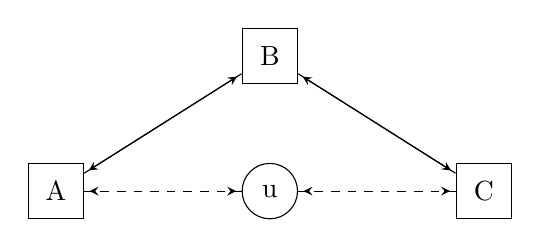
\begin{tikzpicture}[%
    ->,
    shorten >=2pt,
    >=stealth,
    node distance=2cm,
    noname/.style={%
      rectangle,
      minimum width=2em,
      minimum height=2em,
      draw
    }
  ]
  % Nodes:
    \node[noname] (A)                               {A};
    \node[noname] (u) [circle, node distance=2cm, right=of A]   {u};
    \node[noname] (B) [node distance= 1cm, above =of u]        	{B};
    \node[noname] (C) [right=of u]                  {C};
  % Paths:
    \path (A) edge     node [above] {} (B);
    \path (B) edge     node [above] {} (A);
    \path (B) edge     node [above] {} (C);
    \path (C) edge     node [above] {} (B);
    \path[dashed] (u) edge     node [left]  {} (A);
    \path[dashed] (u) edge     node [right] {} (C);
    \path[dashed] (A) edge     node [left]  {} (u);
    \path[dashed] (C) edge     node [right] {} (u);

    %\draw[->] (C) to [bend right] node [above] {?} (A);
\end{tikzpicture}
\end{center}
%------------------------------------------------------------------------





\subsection{Treatment (Causal) Effects, SUTVA, Confounding}

In its simplist form, we care about the difference between the average treated effect and the average control effect. The difference between the two is the \textbf{Naive Differences in Means}, or the naively simple calculation of treatment effects. Why is it naive? Well, we haven't considered any assumptions surrounding the groups, and the fundemental problem of causal inference --- the counterfactual. A counterfactual is the ``what if'' of being in the other group than the one assigned. \index{Naive Differences in Means}

\begin{equation}
\hat{\mu}_\text{Naive} = E[Y|D=1] - E[Y|D=0]
\end{equation}


Think for a second, given all of this, when might the $\hat{\mu}_\text{Naive} = \hat{\mu}_\text{ate}$? Or, when might the naive estimator be the same as our average treatment effect (ATE)? Remember that the reason why $\mu_{naive}$ is naive is because it never oberserves the counterfactual world.
\prac[inline]{Think: Causation, When will the ATE be the same as the Naive Estimator?}

\hfill \\

\noindent \textit{Answer:}\\

Note that the above equation has no decorations on $Y$, we are assuming that all respondents are not interacting with each other, even over time, (SUTVA) and that our design is absolutely complete (think of a complete DAG plot) such that we really are just getting $ E[Y_1] - E[Y_0]$. So no error, and no SUTVA violation we get the $ate$ to equal $\mu_{Naive}$. \index{SUTVA} Here SUTVA is doing a lot of work, we are assuming with SUTVA that there is no interference and treatment variation ($ Y = Y_1)$. This is a pretty monsterous assumption, countries, people, politicians, the media, \textit{everyone} often communicates and shares what they have been ``treated'' with all the time! Beyond this, treatments often effect people very differently depending on affiliaiton, openness to feedback, or if you ate breakfast that morning. Some methods like network analysis will embrace this fact instead of avoiding, although this method will not be covered here.

\hfill \\

\noindent SUTVA, or the Stable Unit Treatment Value Assumption, follows two primary tennants:

\hfill \\

\begin{itemize}
\item[1.] That the treated and controlled units are not interacting between one another.
\item[2.] That the method of how someone gets treated does not varry between units, or is at least eqivelent.
\end{itemize}

\hfill \\

\noindent Some core assumptions are not only SUTVA (consistency) but also that no \textit{confounding} occurs (also known as selection on observables, ignorability). This is when the people that were to benefit most from the treatment select into the treatment. No confounding formally is: \index{confounding} \index{selection on observables} \index{ignorability}

\begin{equation}
D \Vbar Y_1, Y_0 = P(D=1 ~ | ~ Y_1, Y_0)
\end{equation}

This language, by the way, is really annoying because: selection on observables $=$ conditional independence $=$ conditional ignorability $=$ no confounding, conditional on covariates $=$ blocking all back door paths. \index{blocking} \index{selection on observables} \index{back door paths} Open backdoor paths, is Pearlsian DAG-speak for having confounding. If we have more treated folk for each $Y_0$'s than $Y_1$'s then we have imballance. If X is correlated with $Y_1$ and $Y_0$ for \textit{any reason}, then even though we randomized, then $Y_1$ and $Y_0$ would be informative about $X$ - And therefore $Y_1$ and $Y_0$ would be informative about our treatment D! Therefore we have a broken experiment.

Some other things to look out for is the plug-in estimator and conditional expectation functions, each of these are just examining average treatment effects around conditions (control variables). The \textit{plug-in estimator} is when we condition on and control for the average treatment effect (ATE) summing up over our controlled $X$'s.

\begin{equation}
E_X[E[Y |  D = 1, X] − E[Y |D = 0,X]]
\end{equation}

\noindent The conditional expectation function (CEF) is when we take the average treatment effect to see conditional causal effects.

\begin{equation}
E[Y |D] = E[Y_0] + \mu_{ate}D
\end{equation}

We could think about taking into account all variables and possible conditions, this is the hope of Rubin's \textit{saturated model}, which has it's roots in imputation for trying to find missing data (the missing data here in our case would be the counterfactuals). Saturated models do come with particular downsides however, mostly in the errors it produces, and our lack of knowing the exact causal pathway given that adding new variables can open up back-door-paths to our causal estimand. \index{saturated modeling} \index{imputation}


%--------------------------------------------------------------------------------------------------------------
\hfill \\

\subsection{Identification Through Randomization, Hypothesis Testing}

Identification strategies are the attempt to find the missing data that we don't know due to the fundemental problem of causal inference. Two popular paths to do this are using controls and randomization.

There are different types of randomization to help us gain inference. Simple randomization is a probability of treatment per individual ($D$ ``treatment'' being applied) in all possible cases; complete randomization is deciding what fraction of observations we need to fulfil for our total group and then curate our probability of treatment to this. Using randomization, we can hope to ``block'' on these observations (like gender, or X) which we cannot randomally assign.

\begin{equation}
D \Vbar Y_1, Y_0 | X ~ \text{or,} ~ P(D=1 ~ | ~ Y_1, Y_0; X) = p
\end{equation}

\hfill \\

Essentially, we could calculate the naive differences in means for each possible estimation of all of treatment and control groups: and that is called randomization inference (Rubin's causal model).


\hfill \\

In hypothesis testing we could just take with and without treatment and see how our distributions converge (remember the t-test stuff)

\begin{equation}
\sqrt{n}(\hat{\mu} - \mu) \xrightarrow[]{d} \mathcal{N}(0, \sigma^2)
\end{equation}

\index{p-values}
Cool, what's the p-values that we get from this? It is saying that conditional on the null hypothesis (i.e., conditional on $\mu_{ate} = 0$ ), what is the (frequentist) probability of observing this extreme an estimate of $\hat{\mu}$? This is typically in regards to a sharp null hypothesis of zero average effects, $Y_1 = Y_0$ always. \index{sharp null hypothesis}

\prac[inline]{Think: What really is a p-value telling us?}


%------------------------------------------------------------------------------------------

\hfill \\


% Slide 45 of causal 4 has regression components.

%------------------------------------------------------------------------------------------
%    Law of itterated expecations? it is when we take the E[E(Y|D)] we can boil it down to E[Y]
%
Note that our experiments can lose observations rather quickly not only through design but in human execution (for various reasons). Consider the hypothetical flow chart on the following page for a good way to report these losses to readers (often included in supplemental appendix online). This has the added visual benefit of informing readers (reviewers) of your paper's design,


% A CONSORT-style flowchart of a randomized controlled trial
% using the PGF/TikZ package
% Author  : Morten Vejs Willert (July 2010)
% License : Creative Commons attribution license
\newpage
\begin{center}
  % setting the typeface to sans serif and the font size to small
  % the scope local to the environment
  \sffamily
  \footnotesize
  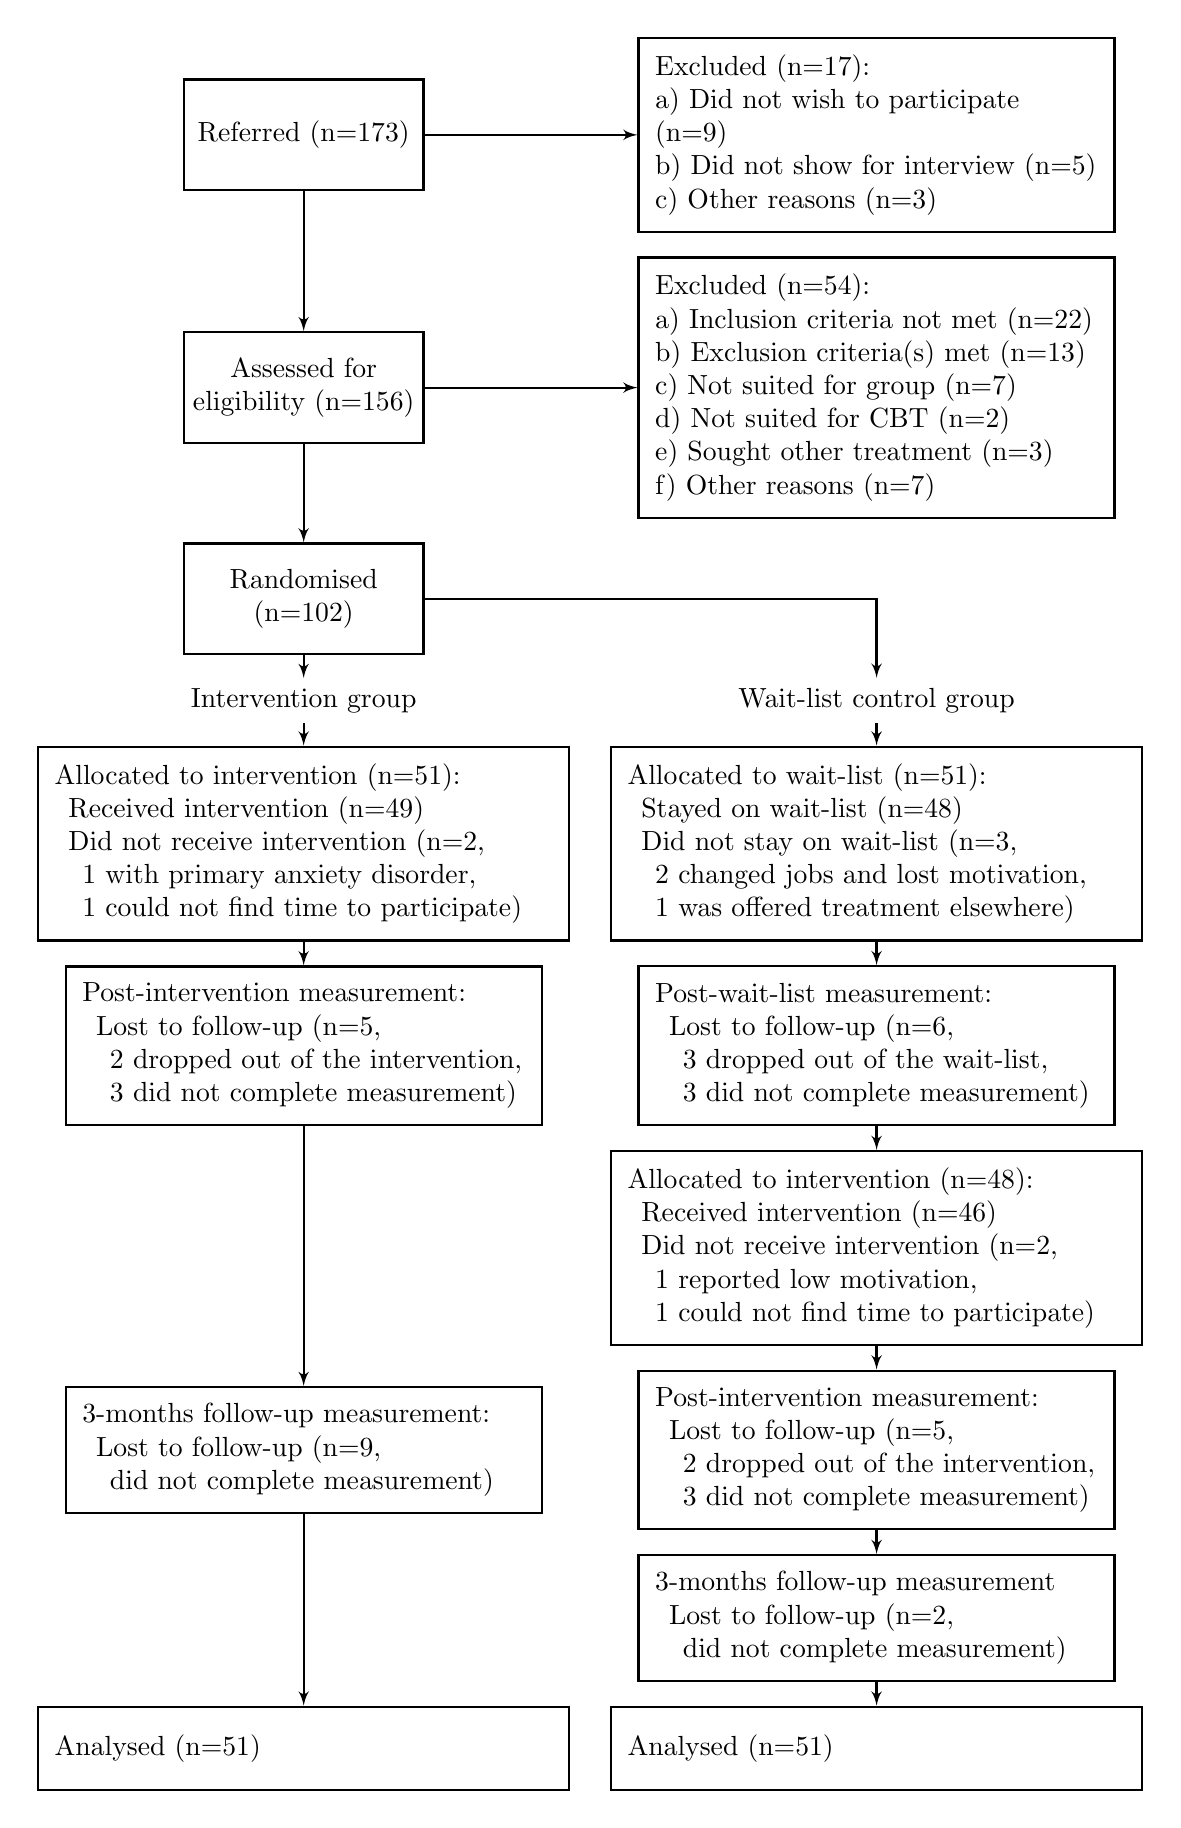
\begin{tikzpicture}[auto,
    %decision/.style={diamond, draw=black, thick, fill=white,
    %text width=8em, text badly centered,
    %inner sep=1pt, font=\sffamily\small},
    block_center/.style ={rectangle, draw=black, thick, fill=white,
      text width=8em, text centered,
      minimum height=4em},
    block_left/.style ={rectangle, draw=black, thick, fill=white,
      text width=16em, text ragged, minimum height=4em, inner sep=6pt},
    block_noborder/.style ={rectangle, draw=none, thick, fill=none,
      text width=18em, text centered, minimum height=1em},
    block_assign/.style ={rectangle, draw=black, thick, fill=white,
      text width=18em, text ragged, minimum height=3em, inner sep=6pt},
    block_lost/.style ={rectangle, draw=black, thick, fill=white,
      text width=16em, text ragged, minimum height=3em, inner sep=6pt},
      line/.style ={draw, thick, -latex', shorten >=0pt}]
    % outlining the flowchart using the PGF/TikZ matrix funtion
    \matrix [column sep=5mm,row sep=3mm] {
      % enrollment - row 1
      \node [block_center] (referred) {Referred (n=173)};
      & \node [block_left] (excluded1) {Excluded (n=17): \\
        a) Did not wish to participate (n=9) \\
        b) Did not show for interview (n=5) \\
        c) Other reasons (n=3)}; \\
      % enrollment - row 2
      \node [block_center] (assessment) {Assessed for eligibility (n=156)};
      & \node [block_left] (excluded2) {Excluded (n=54): \\
        a) Inclusion criteria not met (n=22) \\
        b) Exclusion criteria(s) met (n=13) \\
        c) Not suited for group (n=7) \\
        d) Not suited for CBT (n=2) \\
        e) Sought other treatment (n=3) \\
        f) Other reasons (n=7)}; \\
      % enrollment - row 3
      \node [block_center] (random) {Randomised (n=102)};
      & \\
      % follow-up - row 4
      \node [block_noborder] (i) {Intervention group};
      & \node [block_noborder] (wlc) {Wait-list control group}; \\
      % follow-up - row 5
      \node [block_assign] (i_T0) {Allocated to intervention (n=51): \\
      \h Received intervention (n=49) \\
      \h Did not receive intervention (n=2, \\
      \hh 1 with primary anxiety disorder, \\
      \hh 1 could not find time to participate)};
	  & \node [block_assign] (wlc_T0) {Allocated to wait-list (n=51): \\
      \h Stayed on wait-list (n=48) \\
      \h Did not stay on wait-list (n=3, \\
      \hh 2 changed jobs and lost motivation, \\
      \hh 1 was offered treatment elsewhere)}; \\
      % follow-up - row 6
      \node [block_lost] (i_T3) {Post-intervention measurement: \\
      \h Lost to follow-up (n=5, \\
      \hh 2 dropped out of the intervention, \\
      \hh 3 did not complete measurement)};
	  & \node [block_lost] (wlc_T3) {Post-wait-list measurement: \\
      \h Lost to follow-up (n=6, \\
      \hh 3 dropped out of the wait-list, \\
      \hh 3 did not complete measurement)}; \\
      % follow-up - row 7
      % empty first column for intervention group
      & \node [block_assign] (wlc_T36) {Allocated to intervention (n=48): \\
      \h Received intervention (n=46) \\
      \h Did not receive intervention (n=2, \\
      \hh 1 reported low motivation, \\
      \hh 1 could not find time to participate)}; \\
      % follow-up - row 8
      \node [block_lost] (i_T6) {3-months follow-up measurement: \\
      \h Lost to follow-up (n=9, \\
      \hh did not complete measurement)};
      & \node [block_lost] (wlc_T6) {Post-intervention measurement: \\
      \h Lost to follow-up (n=5, \\
      \hh 2 dropped out of the intervention, \\
      \hh 3 did not complete measurement)}; \\
      % follow-up - row 9
      % empty first column for intervention group
      & \node [block_lost] (wlc_T9) {3-months follow-up measurement \\
      \h Lost to follow-up (n=2, \\
      \hh did not complete measurement)}; \\
      % analysis - row 10
      \node [block_assign] (i_ana) {Analysed (n=51)};
      & \node [block_assign] (wlc_ana) {Analysed (n=51)}; \\
    };% end matrix
    % connecting nodes with paths
    \begin{scope}[every path/.style=line]
      % paths for enrollemnt rows
      \path (referred)   -- (excluded1);
      \path (referred)   -- (assessment);
      \path (assessment) -- (excluded2);
      \path (assessment) -- (random);
      \path (random)     -- (i);
      \path (random)     -| (wlc);
      % paths for i-group follow-up rows
      \path (i)          -- (i_T0);
      \path (i_T0)       -- (i_T3);
      \path (i_T3)       -- (i_T6);
      \path (i_T6)       -- (i_ana);
      % paths for wlc-group follow-up rows
      \path (wlc)        -- (wlc_T0);
      \path (wlc_T0)     -- (wlc_T3);
      \path (wlc_T3)     -- (wlc_T36);
      \path (wlc_T36)    -- (wlc_T6);
      \path (wlc_T6)     -- (wlc_T9);
      \path (wlc_T9)     -- (wlc_ana);
    \end{scope}
  \end{tikzpicture}
\end{center}

\newpage

\noindent On hypothesis testing, in most cases we start off with testing against a \textit{sharp null hypothesis of zero average effects}. That is, $\mu_{ate} = 0$. Note that this is probably the most boring, unrealistic, and uninteresting null hypothesis that we could ever test against. Does anything, in social science, really ever have a sharp zero effect? Probably not, but we use our handy friends, the z-test and t-test, to find the statistical significance of our finding compared to the zero effect. For small samples we often assume that, because of the large sample size used, the unkown population variance may be replaced by the sample variance. That is, instead of a z score we use a t score:

\begin{equation}
z= \frac{\bar{x} - \mu}{\sigma / \sqrt{n}}
\end{equation}

\noindent one would use:

\begin{equation}
t = \frac{\bar{x} - \mu}{s_x / \sqrt{n}}
\end{equation}





\subsection{Frequentism and Bayesianism: What are we really doing here?}

``Statistics'' has its roots, interestingly, in social sciences as the origins of the word derives from ``state-istics'' or the study of the state. This methodology, uniquely bred for States to understand it's citizenry, statistics have become fascinatingly turned for the \textit{people} to now understand their State. Following World War II this was more important than ever, a social science with deep philosophical, theoretical, and qualitative research began to explode with quantiative methodology in through the 1950's. These methodologies, deeply aided by fields like biology, computer science, and econometrics, have both drawn us closer to understanding public and governmental behavior \textit{and} has driven us farther from these concepts as methodology has been misused (e.g. p-hacking), misunderstood, and miscommunicated.

To begin to understand why we use statistics, general linear models, or machine learning, one must first understand a few basic underpinnings of frequentist theory versus Bayesian theory. Frequentism comes in social science largely from R.A. Fisher's idea of likelihood theory of inference. It argues that one true parameter ($\theta$) exists in nature and all scientists are doing are getting multiple samples to guess the one-true-fixed $\theta$. Our results are likelihoods that are close to measuring the one-true DGP but \textbf{always} with some uncertainty. In theory, we can map our estimated DGP $\hat{\theta}$ in two-dimensions pretty easily (think of a basic x--y coordinate grid). Yet, the social world is very complex, as we add more and more variables we begin to get to a point where we find ourselves in hyperspace, unable to map and visualize our surroundings (thus, machine learning helps here, but this will come up later). To help find interesting points when we do these regressions, we (in frequentist theory) seek the MLE or the Maximum Likelihood Estimation. Note this is purposefully not the Maximum \textit{Probabilistic} Estimation, in likelihoodist theory these words mean very different things. The take-away here should be to be careful when speaking in likelihoods (a relative measure of uncertainty) versus probabilities (results only from randomized experiments) as these words have strict definitions in causal inference.

An MLE is interesting because it is the impasse between our estimated parameter $\hat{\theta}$ and our $y$ dependent variable. This typically occurs at the ``highest'' or maximum point on whatever curve we have. Consider the image below, the red line indicates the plateau or maximum point, for the liklihood ($L$) of $y$ (estimated by $x_1$, etc.) on our $\theta$.

\begin{center}
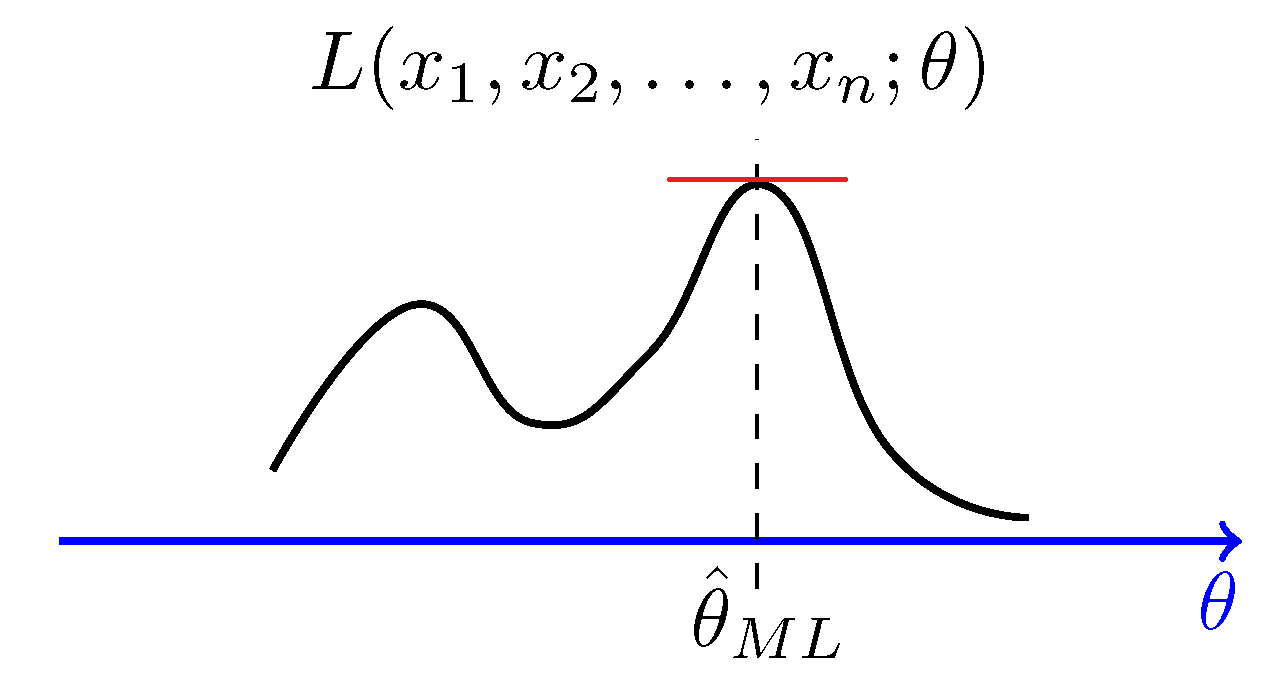
\includegraphics[scale=2]{MLEex}
\end{center}

\clearpage

To find, mathematically, our MLE (which occurs under-the-hood in R) we compute the following: \index{MLE}

\begin{list}{}{}
\item[1.] We $\log$ the likelihood function for ease of computation.
\item[2.] We then take the derivative (also known as the score-function).
\item[3.] Then set this derivative equal to zero (to find our flat top part).
\item[4.] we then solve for $\hat{\theta}$.
\item[5.] We then make sure found the maximum and not some minimum peak (note we could have found the other peak in the above image). To do this we check the sign of the second derivative, if negative we know the curve is downward-facing. We finish by calculating the Fisher information (the second derivative) to find our confidence via variance and standard errors.
\end{list}





\subsection{Running Assumptions}

\prac[inline]{Think: What assumptions are in causal analysis?}

Typically we trade-off assumptions but can never completely eliminate them, only show or \textit{prove} that we have fulfilled them -- all to get closer to causation (causal inference). Some running assumptions are:

\begin{itemize}
\item[1.] SUTVA
\item[2.] No confounding
\item[3.] Probability exists only between 0 and 1, but never zero nor 1.
\end{itemize}

\noindent If we attempt to "lean-into" one of these assumptions to be able to measure it, we may come across additional assumptions like "parrallel paths" or various representation and error assumptions. Some of these will be discussed in the Regression section of this book.


\subsection{Non-parametric Modeling}

A few non-parametric models help us lean away from certain assumptions. This could be an entire class on it's own, but I have a few notes that I'll share here.


\subsubsection{Multiple Comparisons}


\subsubsection{Marginal Structural Models (MSM)}
\index{Marginal Structural Modeling}

If we are working with relational datasets, and do have downstream effects at $t_1$, $t_2$, $t_n$ we cannot solve this problem by using fixed effects. Because we are assuming with fixed effects that our estimands do not change over time, this is actually a core assumption that is violated all the time. However, fear not, for marginal structural models can help us when fixed effects cannot.

Assuming time doesn't influence previous times (which may be an issue if we're studying some forecasting or strategic process that appears in our data). we can look at the outcome in th elast time period and stack each time period on top of one another. This is very different from adding a bunch of dummy variables, it is stacking the time periods together; we can treat for the histories in this way and potential influence amongst them.\footnote{It may be a good idea to check out time series analysis here, just in case you problems can be solved with your data.}

So marginal structural models can work with different treatment histories (arms) than fixed effects. Let's fit a model for every ``D,'' and just weight each of these down the road. We conditionon the history of past events, and if the model pukes at us then we drop the bad cases and redefine the subsample we are talking about, and how it's still interesting.

Note, we do not get out of the unobservables problem, we still need to set up this model with the same theory and careful design. \textit{You cannot analyize your way out of a bad design. }

Some code to look into, (and notes):

\begin{knitrout}
\definecolor{shadecolor}{rgb}{0.165, 0.169, 0.184}\color{fgcolor}\begin{kframe}
\begin{alltt}
\hlstd{> }\hlcom{# GLM has an argument called "weights," don't trust it...}
\hlstd{> }
\hlstd{> }\hlkwd{library}\hlstd{(survey)} \hlcom{# this is better for a variety of reasons.}
\hlstd{> }     \hlkwd{svydesign}\hlstd{(}\hlkwc{ids} \hlstd{= ,} \hlkwc{weights} \hlstd{=} \hlopt{~}\hlnum{1}\hlstd{, data)}
\hlstd{> }     \hlkwd{svyglm}\hlstd{( Y} \hlopt{~} \hlstd{D, unweighted_design,} \hlkwc{family} \hlstd{= quasibinomial)}
\hlstd{> }     \hlkwd{coef}\hlstd{(The_Model)}
\end{alltt}
\end{kframe}
\end{knitrout}

These weighted coefficents can help us, but we can try to stabilize teh weights we get, especially in cases of low probability events. For this we need non-dynamic probabilities. Assign these values with R's ``mgcv'' package, and function ``bam'' and some smoothing with \texttt{s()}. Get the t-specific weights, and there are ways to plot the improvements  from doing this. Then, put the weights together (stabilized) so mean aroudnd 1, and multiply these easily with \texttt{prod(weights)}. Change out these weights in above, instead of \texttt{1} we can use \texttt{ weights}:

\begin{knitrout}
\definecolor{shadecolor}{rgb}{0.165, 0.169, 0.184}\color{fgcolor}\begin{kframe}
\begin{alltt}
\hlstd{> }\hlcom{# after checking out:}
\hlstd{> }\hlkwd{library}\hlstd{(mgcv)}
\hlstd{> }     \hlkwd{bam}\hlstd{()}
\hlstd{> }     \hlkwd{s}\hlstd{()}
\hlstd{> }
\hlstd{> }\hlcom{# Then we can edit things:}
\hlstd{> }\hlkwd{library}\hlstd{(survey)} \hlcom{# this is better for a variety of reasons.}
\hlstd{> }     \hlkwd{svydesign}\hlstd{(}\hlkwc{ids} \hlstd{= ,} \hlkwc{weights} \hlstd{=} \hlopt{~}\hlstd{weights, data)}
\hlstd{> }     \hlkwd{svyglm}\hlstd{( Y} \hlopt{~} \hlstd{D, weighted_design,} \hlkwc{family} \hlstd{= quasibinomial)}
\hlstd{> }     \hlkwd{coef}\hlstd{(The_Model)}
\hlstd{> }
\hlstd{> }     \hlcom{# Might wan to check out package: cbmsm}
\end{alltt}
\end{kframe}
\end{knitrout}

We can then get predicted probabilities from our marginal structural models. So essentially with marginal structural models:

\begin{itemize}
\item[1.] Set up data so each outcome has multiple individuals and prior time periods.
\item[2.] Model treatment in each period without tie-varying covariates with them.
\item[3.] Asses ballance (repeat 2 if necessary).
\item[4.] stabilize weights.
\item[5.] calculate weighted estimates of QOI's.
\item[6.] What is N anymore? Let's just always bootstrap the heck out of this: doing (2), (4), (5), over 1,000 times over.
\end{itemize}

\hfill \\
\hfill \\

%------------------------------------------------------------

\subsection{Finding Causal Estimands:}

\hfill \\

\subsubsection{Matching and Propensity Scores:}

\textbf{Matching is weighting} each observation to all strata. Much of this is really the same thing, matching is pairing individuals and comparing causal estimands and weighting is forcefully multiplying a ``weight'' onto our variables to pair them to reality (say the Census). Subclassifcation is the same thing, in the long, as matching and weighting. If we don't have exact matches we can use a coarse matching approach where we break up a continuous variable into deciles. This is similar to K-Nearest Neighbor subclassification matching. \index{matching} And a propensity score is just the probability of treatment given some X. \index{propensity scores}

\begin{equation}
e(X) = Pr(D = 1|X)
\end{equation}

The idea is then to coarsen/subclassify or nearest-neighbor match on the \textbf{propensity score}. \index{coarse matching} \index{nearest-neighbor} \textbf{Subclassification} is making the probabilities of treatment and controll equivilant in observational studies. Doing this, we help create ballance in our treated and controlled groups. This is similar to complete randomization in experimental trials. (What machine learning techniques can help us here?) \index{subclassification}

Some machine learning approaches that can help us here (see machine learning chapter for more) include regression trees and other classification approaches. These can help us identify groups to match on create more ballance in our data.




\hfill \\

\subsubsection{Fixed Effects:}

Fixed effects are dummy varriables (are stratification) and are turning ``on or off'' a year, country, or some other theoretically interesting variable to ``account'' for the things that pour into a time or place. Using this we assume no carry over between years to previous or future years. Here are the assumptions with fixed effects: \index{Fixed Effects} \index{Marginal Structural Models}

\hfill \\

\begin{itemize}
\item[1.] no unobserved time-varying confounder exists
\item[2.] past outcomes do not directly affect current outcome
\item[3.] past outcomes do not directly affect current treatment
\item[4.] past treatments do not directly affect current outcome
\end{itemize}

\hfill \\

\noindent One larger problem is that the linear fixed effect does not consistently estimate the ATE:

\begin{equation}
\beta_{LFE} \rightarrow \frac{E[V^i \mu^i_{naive}]}{E[V^i]} \neq \mu_{ate}
\end{equation}

\noindent But marginal structural models allow for our times and events to influence one another (more on that later).


\hfill \\

\subsubsection{Differences in Differences}
\index{Differences in Differences}
Differences in Differences is a way to estimate our causal estimand (ATT, ATE, etc) and map it when treatment rolls out. Say we have three time points 1, 2, and 3, where all are untreated at 1, some are treated at 2, and all are treated at 3. To get the estimand from differences in differences we first subtract (getting the difference) of the mean outcomes between times and 2 and time 1 for the treated and controlled then calculate the differences in those two groups between the two time groups. We could do the same thing for 3 and 2. An assumption for difference in differences designs is that things were to be on the same parallel paths, or that we need to prove to the reader (often through theory) that the treated and controlled group -- in a world where no treatment occured, actually would've been the same (parrallel to one another). Further, that it is only our treatment group that caused a change between the control and treated group, not anything that would've happened anyways.

\hfill \\

\subsubsection{Instrumental Variables}

Here imagine we are interested in the causal effect of D --> Y but our errors, or some unknown (u) covariate influences both our treatment and outcome. What we can do is add in some "garbage" variable (Z) into the mix, and see just how Z passes through to Y. It helps me think of "pipes" where we want to see how much [insert liquid here] passes through D to Y, neverminding covariate u.

\begin{center}
\begin{tikzpicture}[%
    ->,
    shorten >=2pt,
    >=stealth,
    node distance=3cm,
    noname/.style={%
      rectangle,
      minimum width=2em,
      minimum height=2em,
      draw
    }
  ]
  % Nodes:
    \node[noname] (Z)                                   {Z};
    \node[noname] (D) [node distance=2cm, right=of Z] {D};
    \node[noname] (Y) [right=of D]        				{Y};
    \node[noname] (u) [circle, node distance=2cm, above right=of D] {u};
  % Paths:
    \path (D) edge     node {} (Y)
          (Z) edge     node {} (D)
          (u) edge     node {} (D)
          (u) edge     node {} (Y);
\end{tikzpicture}
\end{center}
\hfill
















%----------------------------------------------------------------------------------
\clearpage
\section{Survey Design}
\hfill \\

\subsection{The Survey Experiment}

\subsection{Types of Questions}

\subsection{Psychology of Design}



\hfill \\
\subsubsection{The "Don't Know" Option:}



\subsection{Useful Rules of Thumb}

\subsection{Research on Survey Biases}


\clearpage
%-----------------------------------------------------------------------------------










\clearpage
\section{Regression:}

\begin{equation}
\mathlarger{ y = \beta_0 + \beta X + \epsilon }
\end{equation}

The General Linear Model (GLM) consists of a \textit{stochastic and systematic} components. The stochastic component is the section in the equation which changes (``randomly'') and has error our error term ($\epsilon$), whereas the systematic component remains constant with data values ($X$) and is used to test our dependent variable ($y$) and give us interpretive values in the form of coefficients ($\beta$). To ``generalize'' this to other models (as we'll see in this document) we need a distribution and a link function, which will come up later.

It should be mentioned that this GLM formula has it's genesis in basic geometry's equation for a line $y=mx + b$ the root of this should be intuitive as we attempt to fit a line to our data and estimate it using maximum likelihood.

No matter what the model we're specifying throughout this document, be it logit, probit, Poisson, or survival models the linear predictor will always be the same:

\begin{equation}
\mathlarger{ \eta = X\beta \text{ \text{  }  or,  }}
\mathlarger{ \eta_i = \beta_0 + \beta_1 x_{i1} \textbf{...} \beta_q x_{iq}  }
\end{equation}
\prac{Set up a problem here}
One example of when we might use regression is when trying to determine the best quality of beer based upon mean judged ratings, these are the questions that matter the most. Beer ratings range from $-1$: ``Fair'', to $0$: ``Good'', and $1$: ``Great.'' Consider our first model where we consider how expensive the beer is:

\begin{equation}
\mathlarger{ \text{Beer Rating} = \beta_0 + \beta \text{Beer Price} + \epsilon }
\end{equation}

\noindent Given the information from our data regressed in R: (This is shown on the following page)

\begin{equation}
\mathlarger{ \text{Beer Rating} =  (-0.76) + (.26) \text{Beer Price} + \text{error} }
\end{equation}

We can solve this to find our beer rating with the substitution of a beer price, we remove the error term because we assume it's normally distributed and centered at zero (an assumption that will come up in the following section). Let's assume we are going out with friends and only have \$2.00:

\begin{equation}
\mathlarger{  \text{Beer Rating} = (-0.76)+(.26)\cdot 2.00 = -.24 }
\end{equation}

This means, given that our average (``Good'') beer rating is zero, that if we only had two dollars to spend on a beer we would get a slightly below average beer ($-.24$). This is assuming the price of beer and rating of beer is a linear relationship, this isn't an assumption we always have to make but one we will for now.

\clearpage
\noindent Showing this in R, let's load and set up our data and run the model that we used to get the numbers above: \index{loading data} \index{recoding data}
\begin{knitrout}
\definecolor{shadecolor}{rgb}{0.165, 0.169, 0.184}\color{fgcolor}\begin{kframe}
\begin{alltt}
\hlstd{> }\hlcom{## Initial pass: reading data, looking at variables.}
\hlstd{> }\hlcom{# Data available, email: MailKyleDavis@gmail.com}
\hlstd{> }
\hlstd{> }\hlkwd{library}\hlstd{(foreign)} \hlcom{# For reading data.}
\hlstd{> }\hlstd{beer_data} \hlkwb{<-} \hlkwd{read.dta}\hlstd{(}\hlstr{'C:/Users/Shing/Documents/Previous Course Info/Quant II/beer.dta'}\hlstd{)}
\hlstd{> }
\hlstd{> }\hlkwd{library}\hlstd{(car)} \hlcom{# for ease of recoding variables}
\hlstd{> }\hlcom{# Our Beer ratings could be coded more intuitively:}
\hlstd{> }\hlstd{beer_data}\hlopt{$}\hlstd{rating} \hlkwb{<-} \hlkwd{as.numeric}\hlstd{(beer_data}\hlopt{$}\hlstd{rating)}
\hlstd{> }\hlkwd{head}\hlstd{(beer_data)} \hlcom{# Check out the variables we have available to us:}
\end{alltt}
\begin{verbatim}
##   rating         beer  origin avail price cost calories sodium alcohol
## 1      1 Anchor Steam     USA     1  7.19 1.20      154     17     4.7
## 2      1      Labatts  Canada     1  3.15 0.53      147     17     5.0
## 3      1       Molson  Canada     1  3.35 0.56      154     17     5.1
## 4      1    Budweiser     USA     0  2.59 0.43      144     15     4.7
## 5      1     Heineken Holland     0  4.59 0.77      152     11     5.0
## 6      1  Kronenbourg  France     1  4.39 0.73      170      7     5.2
##      class    light us quality good verygood
## 1 Super-pr NONLIGHT  1       3    1        1
## 2  Premium NONLIGHT  0       3    1        1
## 3  Premium NONLIGHT  0       3    1        1
## 4  Premium NONLIGHT  1       3    1        1
## 5 Super-pr NONLIGHT  0       3    1        1
## 6 Super-pr NONLIGHT  0       3    1        1
\end{verbatim}
\begin{alltt}
\hlstd{> }\hlkwd{nrow}\hlstd{(beer_data)} \hlcom{# For 35 beers:}
\end{alltt}
\begin{verbatim}
## [1] 35
\end{verbatim}
\begin{alltt}
\hlstd{> }\hlcom{# Let's recode our rating dependent variable to be more intuitive:}
\hlstd{> }\hlcom{# reassign values: where 3 is now 0, etc..}
\hlstd{> }\hlstd{beer_data}\hlopt{$}\hlstd{rating} \hlkwb{<-} \hlkwd{recode}\hlstd{(beer_data}\hlopt{$}\hlstd{rating,}\hlstr{"3=0; 2=1; 1=2"}\hlstd{)}
\hlstd{> }\hlkwd{class}\hlstd{(beer_data}\hlopt{$}\hlstd{rating)} \hlcom{# numeric and coded intuitively, could be better...}
\end{alltt}
\begin{verbatim}
## [1] "numeric"
\end{verbatim}
\begin{alltt}
\hlstd{> }\hlcom{# From -1 to 1}
\hlstd{> }\hlstd{beer_data}\hlopt{$}\hlstd{rating} \hlkwb{<-} \hlkwd{recode}\hlstd{(beer_data}\hlopt{$}\hlstd{rating,}\hlstr{"0=-1"}\hlstd{)}
\hlstd{> }\hlstd{beer_data}\hlopt{$}\hlstd{rating} \hlkwb{<-} \hlkwd{recode}\hlstd{(beer_data}\hlopt{$}\hlstd{rating,}\hlstr{"1=0"}\hlstd{)}
\hlstd{> }\hlstd{beer_data}\hlopt{$}\hlstd{rating} \hlkwb{<-} \hlkwd{recode}\hlstd{(beer_data}\hlopt{$}\hlstd{rating,}\hlstr{"2=1"}\hlstd{)}
\hlstd{> }
\hlstd{> }\hlstd{beer_data}\hlopt{$}\hlstd{rating} \hlcom{# Setting median to zero will help our interpretation}
\end{alltt}
\begin{verbatim}
##  [1]  1  1  1  1  1  1  1  1  1  1  1  0  0  0  0  0  0  0  0  0  0  0  0  0
## [25]  0 -1 -1 -1 -1 -1 -1 -1 -1 -1 -1
\end{verbatim}
\end{kframe}
\end{knitrout}


\begin{knitrout}
\definecolor{shadecolor}{rgb}{0.165, 0.169, 0.184}\color{fgcolor}\begin{kframe}
\begin{alltt}
\hlstd{> }\hlkwd{set.seed}\hlstd{(}\hlnum{12345}\hlstd{)} \hlcom{# Setting our seed will fix the randomness for replication}
\hlstd{> }
\hlstd{> }\hlcom{#    Let's do the basic linear model thing:}
\hlstd{> }\hlcom{##!  lm(Y ~ X, data selection)}
\hlstd{> }\hlstd{mod1} \hlkwb{<-} \hlkwd{lm}\hlstd{(rating} \hlopt{~} \hlstd{price,} \hlkwc{data} \hlstd{= beer_data)}
\hlstd{> }\hlcom{# just list our coefficients (to see everything use summary(mod1))}
\hlstd{> }\hlstd{mod1}\hlopt{$}\hlstd{coefficients}
\end{alltt}
\begin{verbatim}
## (Intercept)       price 
##  -0.7561396   0.2592005
\end{verbatim}
\end{kframe}
\end{knitrout}


\begin{knitrout}
\definecolor{shadecolor}{rgb}{0.165, 0.169, 0.184}\color{fgcolor}\begin{kframe}
\begin{alltt}
\hlstd{> }\hlcom{# Texreg Tables:}
\hlstd{> }\hlkwd{library}\hlstd{(texreg)}
\hlstd{> }
\hlstd{> }\hlkwd{texreg}\hlstd{(}\hlkwc{l}\hlstd{=} \hlkwd{list}\hlstd{(mod1),} \hlkwc{stars} \hlstd{=} \hlkwd{numeric}\hlstd{(}\hlnum{0}\hlstd{),}
\hlstd{+ }       \hlkwc{custom.coef.names}    \hlstd{=} \hlkwd{c}\hlstd{(}\hlstr{"Intercept"}\hlstd{,} \hlstr{"Beer Price"}\hlstd{),}
\hlstd{+ }       \hlkwc{caption.above}        \hlstd{= T,} \hlkwc{float.pos} \hlstd{=} \hlstr{"h!"}\hlstd{,}
\hlstd{+ }       \hlkwc{custom.note}          \hlstd{=} \hlstr{"Dependent variable: Beer Rating"}\hlstd{)}
\end{alltt}
\end{kframe}
\end{knitrout}


\begin{table}[h!]
\caption{Statistical models}
\begin{center}
\begin{tabular}{l c }
\hline
 & Model 1 \\
\hline
Intercept  & $-0.76$  \\
           & $(0.36)$ \\
Beer Price & $0.26$   \\
           & $(0.11)$ \\
\hline
R$^2$      & 0.14     \\
Adj. R$^2$ & 0.11     \\
Num. obs.  & 35       \\
RMSE       & 0.74     \\
\hline
\multicolumn{2}{l}{\scriptsize{Dependent variable: Beer Rating}}
\end{tabular}
\end{center}
\end{table}

\index{texreg package}


The above table shows the standard errors (in parentheses) being two standard errors away from our coefficients, therefore being significant at the 95\% confidence level. We have 35 observations and our $\text{R}^2$ explains 14\% of the variation in our dependent variable. The adjusted $\text{R}^2$ accounts for the amount of variables added into a model and is slightly more robust, prevent against ``kitchen sink'' models which add many variables to get a high  $\text{R}^2$. It explains 11\% of the variation.
\index{R$^2$}

Our intercept is when all else is held at zero ($\beta_0$) so the most average priced beer has a rating of $-.76$, which is overall pretty poor quality beer. Yet, if we spend one dollar more, our ranking jumps by .26 (a quarter rank) each time. This can be visually represented alongside simulations in a plot here: \\
\index{Simulation}

\index{base-R plotting}
\begin{center}
\begin{knitrout}
\definecolor{shadecolor}{rgb}{0.165, 0.169, 0.184}\color{fgcolor}\begin{kframe}
\begin{alltt}
\hlstd{> }\hlkwd{library}\hlstd{(arm)} \hlcom{# For sim()}
\hlstd{> }\hlcom{# Let's plot a simulation:}
\hlstd{> }\hlkwd{plot}\hlstd{(beer_data}\hlopt{$}\hlstd{price,} \hlkwd{jitter}\hlstd{(beer_data}\hlopt{$}\hlstd{rating),} \hlkwc{pch}\hlstd{=}\hlnum{19}\hlstd{,}
\hlstd{+ }     \hlkwc{xlab}\hlstd{=} \hlstr{"Price"}\hlstd{,}
\hlstd{+ }     \hlkwc{ylab}\hlstd{=} \hlstr{"Rating"}\hlstd{,}
\hlstd{+ }     \hlkwc{main}\hlstd{=} \hlstr{"Rating by Price of Beer: with 100 simulations"}\hlstd{)}
\hlstd{> }\hlkwd{abline}\hlstd{(mod1)}  \hlcom{# Add our model line}
\hlstd{> }\hlcom{# Simulate 100 possible outcomes, take their lines, plot them on top}
\hlstd{> }\hlstd{m1sim} \hlkwb{<-} \hlkwd{sim}\hlstd{(mod1)}
\hlstd{> }\hlkwa{for} \hlstd{(i} \hlkwa{in} \hlnum{1}\hlopt{:}\hlnum{100}\hlstd{)\{}
\hlstd{+ }  \hlkwd{curve} \hlstd{(}\hlkwd{coef}\hlstd{(m1sim)[i,}\hlnum{1}\hlstd{]} \hlopt{+} \hlkwd{coef}\hlstd{(m1sim)[i,}\hlnum{2}\hlstd{]}\hlopt{*}\hlstd{x,} \hlkwc{add}\hlstd{=T,} \hlkwc{col}\hlstd{=}\hlstr{"grey"}\hlstd{)}
\hlstd{+ }\hlstd{\}}
\hlstd{> }\hlkwd{curve} \hlstd{(mod1}\hlopt{$}\hlstd{coef[}\hlnum{1}\hlstd{]} \hlopt{+} \hlstd{mod1}\hlopt{$}\hlstd{coef[}\hlnum{2}\hlstd{]}\hlopt{*}\hlstd{x,} \hlkwc{add}\hlstd{=T,} \hlkwc{lwd}\hlstd{=}\hlnum{3}\hlstd{)}
\end{alltt}
\end{kframe}
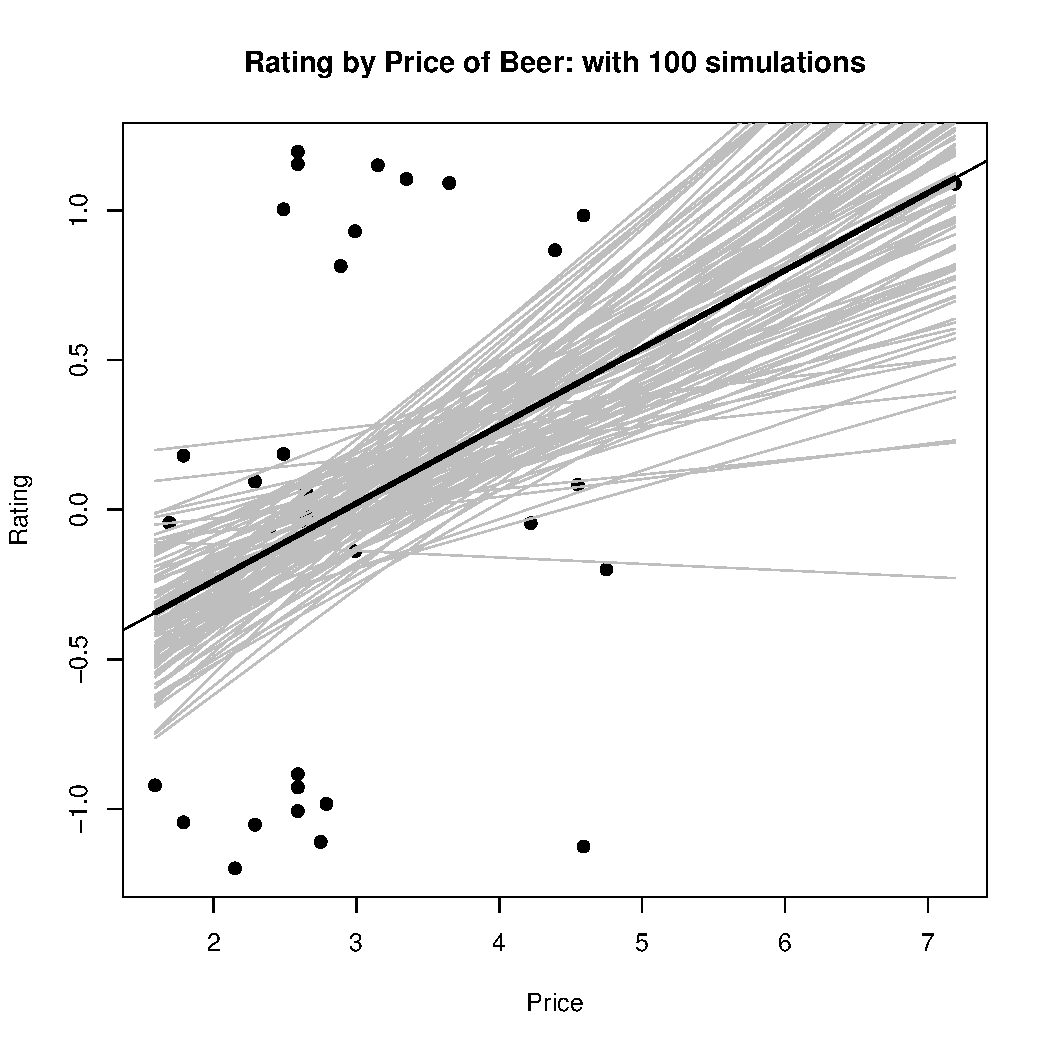
\includegraphics[width=4in]{figure/simulation1-1} 

\end{knitrout}
\end{center}

The grey lines here are simulations which display our confidence intervals around the black regression line for our model. They occupy a low amount of the variation in our dots so intuitively we can see how this would yield a low $\text{R}^2$ (our model only had $.14$). See below:

\begin{knitrout}
\definecolor{shadecolor}{rgb}{0.165, 0.169, 0.184}\color{fgcolor}\begin{kframe}
\begin{alltt}
\hlstd{> }\hlstd{mod2} \hlkwb{<-} \hlkwd{lm}\hlstd{(d}\hlopt{$}\hlstd{rating} \hlopt{~} \hlstd{d}\hlopt{$}\hlstd{price} \hlopt{+} \hlstd{d}\hlopt{$}\hlstd{alcohol)}
\hlstd{> }
\hlstd{> }\hlkwd{texreg}\hlstd{(}\hlkwc{l}\hlstd{=} \hlkwd{list}\hlstd{(mod1, mod2),} \hlkwc{stars} \hlstd{=} \hlkwd{numeric}\hlstd{(}\hlnum{0}\hlstd{),}
\hlstd{+ }       \hlkwc{custom.coef.names} \hlstd{=} \hlkwd{c}\hlstd{(}\hlstr{"Intercept"}\hlstd{,} \hlstr{"Beer Price"}\hlstd{,} \hlstr{"Alcohol Content"}\hlstd{),}
\hlstd{+ }       \hlkwc{caption.above} \hlstd{= T,} \hlkwc{float.pos} \hlstd{=} \hlstr{"h!"}\hlstd{,}
\hlstd{+ }       \hlkwc{custom.note} \hlstd{=} \hlstr{"Dependent variable: Beer Rating"}\hlstd{)}
\end{alltt}
\end{kframe}
\end{knitrout}


\begin{table}[h!]
\caption{Statistical models}
\begin{center}
\begin{tabular}{l c c }
\hline
 & Model 1 & Model 2 \\
\hline
Intercept       & $-0.76$  & $-2.89$  \\
                & $(0.36)$ & $(0.91)$ \\
Beer Price      & $0.26$   & $0.21$   \\
                & $(0.11)$ & $(0.11)$ \\
Alcohol Content &          & $0.50$   \\
                &          & $(0.20)$ \\
\hline
R$^2$           & 0.14     & 0.28     \\
Adj. R$^2$      & 0.11     & 0.23     \\
Num. obs.       & 35       & 35       \\
RMSE            & 0.74     & 0.69     \\
\hline
\multicolumn{3}{l}{\scriptsize{Dependent variable: Beer Rating}}
\end{tabular}
\end{center}
\end{table}

We could consider a model where alcohol content is additionally important, Model 2. Here our R$^2$ increases to .28; and our variables remain within two deviations of the error, with the slight exception of beer price. Our intercept loses it's interpretation, we are now looking at where alcohol content is at zero. Our beer rank jumps by .50 every one increase in alcohol content. Both of these effects are controlling for the other.












%----------------------------------------------------------------------------------------------

\clearpage
\subsection{Modeling Assumptions, Diagnostics}
\hfill \\
In social science empirical research there is no dearth of modeling errors. The following diagnostics and error-checking may not seem worthwhile because this work rarely makes it into the actual publication; but rather into a supplemental appendix. This work too helps a lot to ease skeptical readers about the claims we make (helping us get published).

\begin{equation}
\mathlarger{  \epsilon_i  \thicksim \mathcal{N}(0, \sigma^2)             }
\end{equation}
\noindent \textit{Errors are Normally Distributed}\\
We assume that the errors are normally distributed, to check for this histograms can give us a first pass, but one can also map the residuals and (hopefully) see their ``random'' distribution with no foreseeable trends. the \texttt{plot(model)} command in R can give a few of these plots in a row pretty easily too. Consider our beer rankings model from earlier: \\
\hfill \\

\begin{center}
\begin{knitrout}
\definecolor{shadecolor}{rgb}{0.165, 0.169, 0.184}\color{fgcolor}\begin{kframe}
\begin{alltt}
\hlstd{> }\hlkwd{par}\hlstd{(}\hlkwc{mfrow}\hlstd{=}\hlkwd{c}\hlstd{(}\hlnum{2}\hlstd{,}\hlnum{2}\hlstd{))} \hlcom{# plot multiple alongside each other:}
\hlstd{> }\hlkwd{plot}\hlstd{(mod1)}        \hlcom{# plot our quick model checks}
\end{alltt}
\end{kframe}
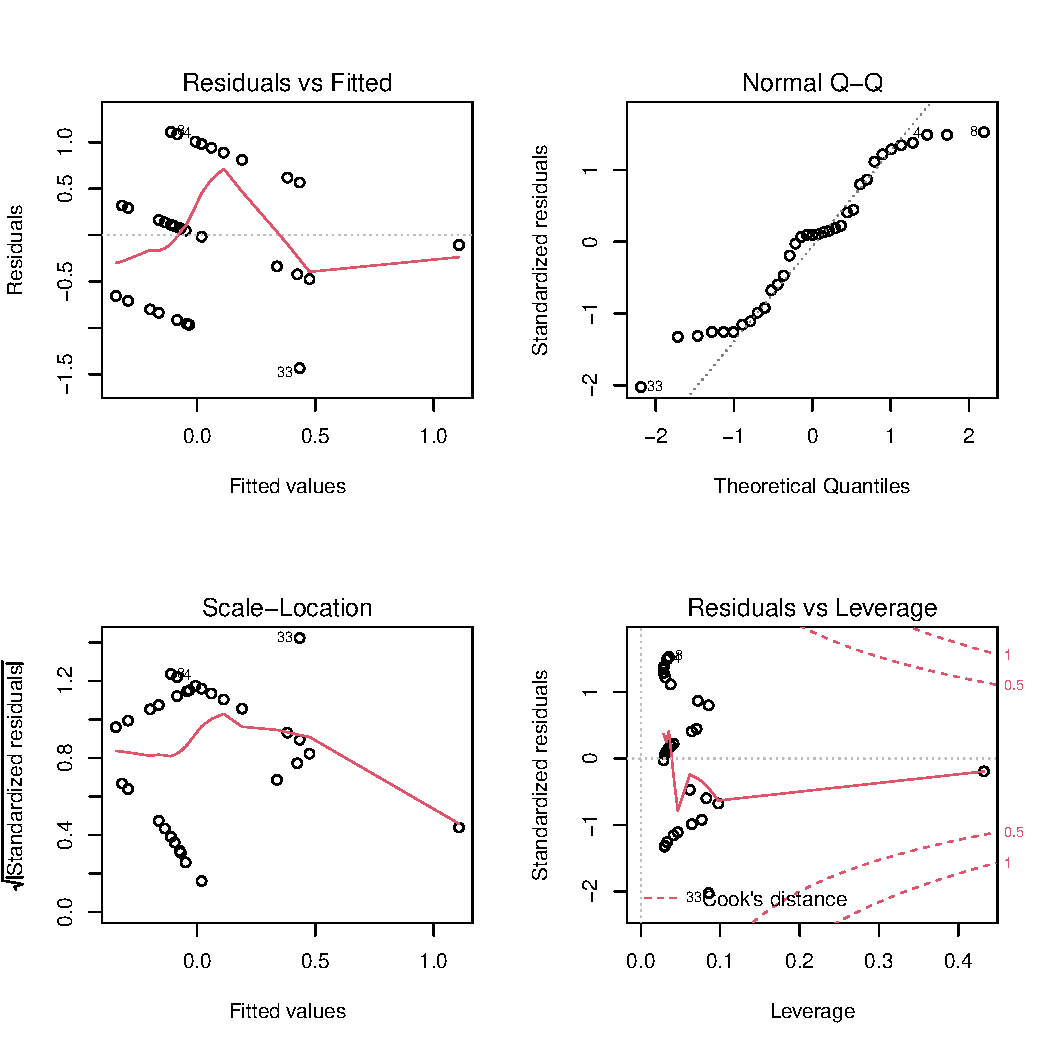
\includegraphics[width=5in]{figure/checkinglinear-1} 
\begin{kframe}\begin{alltt}
\hlstd{> }\hlkwd{par}\hlstd{(}\hlkwc{mfrow}\hlstd{=}\hlkwd{c}\hlstd{(}\hlnum{1}\hlstd{,}\hlnum{1}\hlstd{))} \hlcom{# Reset plotting option}
\end{alltt}
\end{kframe}
\end{knitrout}
\end{center}
\index{checking linear models}

\noindent \textit{Bias in Error}\\
Next, we assume that there is no bias in our errors, meaning that our expectation of our errors in zero: $\text{E}(\epsilon_i) = 0$. It is rare to get exactly zero, but we should report exactly what our errors are and be sure to mention any outliers, leverage points, or otherwise influential points to the reader so they are not mislead. We can handle these situations in various ways:\\
 \textbf{Never outright delete data points.} Theoretically, the social world is vastly complex and rarities can (and do) exist in nature. If we have an influential point, where our data point(s) are not necessarily malicious or supremely rare, but rather pull our analysis in one way or another we can transform all of the data points (log or rescale the variable) to decrease the influence of one point. Observing points outside of ``Cook's Distance'' (in plot R command) can be a good way to observe influential points or outliers. \\
\hfill \\

\noindent \textit{Uniform Variance}\\
Our $\sigma^2$ is not subscripted, meaning we expect a uniform variance in our error term, where there is no increasing or decreasing in our errors. homoscedasticity here is a good thing, we can detect this by plotting our residuals and seeing random variance of our points across the mid-point. We do not want to see heteroscedasticity or where errors funnel outward or have a certain trend in themselves.

\hfill \\
\noindent \textit{Autocorrelation, iid}\\
We do not want our observations to correlate with one-another, meaning our individuals or observations are not influencing another individual respondent's results. Each data point should be independent draws from one another.

\hfill \\
\noindent \textit{Measurement Error (X)}\\
We need to make sure the phenomenon we wish to measure is actually being measured by our data. A question such as ``What do you think about healthcare'' can be responded by a battery of cognitive processes; but a question like ``To what degree of anger do you feel about the current healthcare policy?'' is far more precise to the theoretical process we care to study. Beyond theory, the scale of our variable and our operationalization can be changed and shifted to answer different questions. In Section 3 that follows, for example, we will dichotomize a variable to observe a different question about how we think about our beer rankings.

\clearpage
\hfill \\
\noindent \textit{Omitted Variable Bias (OVB)}
\end{flushleft}

\begin{wrapfigure}{R}{.4\textwidth}
\centering
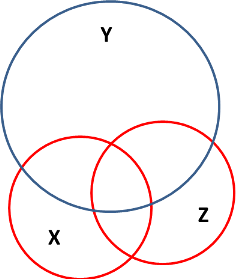
\includegraphics[width=0.25\textwidth]{OVB}
\end{wrapfigure}
OVB occurs when both a a variable excluded from analysis (Z) both theoretically overlaps some of the variance in our dependent variable (Y) and another included variable (X). If Z only overlapped with Y excluding it would just lower our R$^2$ and we would lose some of our potential ability to explain our DV. If Z only overlapped our X variable then we need only acknowledge Z in theory. It is only when Z overlaps both that we run into problems, for both we lose explanation of our DV and we over-inflate the significance of X's influence on Y. This can (and always should) be corrected by building a model slowly, one variable at a time, alongside well thought theory to ensure accuracy and purpose in our problem solving.

\begin{flushleft}
\setlength{\parindent}{1cm} % 1cm indent reitterated after /wrapfigure

\noindent \textit{Parametric Linearity}\\
If we run a standard linear regression we should be sure that our theory informs the decision that this phenomenon is linear, but also check that our relationship between our variables is linear in nature too. Other modifications of the GLM framework can include non-linear distributions. Linearity in our variables can be aided via transformation, with a drawback being (potentially) in interpretation.

\hfill \\
\noindent \textit{Mathematical Concerns}\\
We should ensure that X and Y have enough variance to provide enough change for analysis. Also, we should ensure (as often as we can) that our number of observations (N) is larger than our parameters (K). While having too high of an N will be more likely to report significant results in nearly any scattering of points, too low of an N can either show sharply significant results or no results at all when the \textit{truth} can be the opposite. Typically having an N of 2,000 has been an accepted threshold.

\hfill \\
\noindent \textit{In Structure}\\
We also assume that our model is fully specified, and that our perameters ($\beta$) are ``fixed'' where our variables don't have a change-time or some external influence at a point in the data collection.

\hfill \\
\noindent \textit{Other Notes on Stochastic Robustness}

Note that much of the explainability and diagnostics of our model can be partially examined (at least as a first pass) through our R$^2$. Our R$^2$ is the amount of variance captured in Y from our model. More formally:
\begin{equation}
\mathlarger{ \text{R}^2 = 1 - \frac{\text{RSS}}{\text{TSS}} = 1- \frac{\Sigma \epsilon^{2}_i}{\Sigma\left(Y_i - \bar{Y}\right)^2} }
\end{equation}
This shows our amount of variance explained by our model, over what's unexplained. This quotient is subtracted by one, we get a pretty good interpretation from .00 to 1 where we explain nothing to explaining everything. Other forms significance tests can penalize models for including many variables both linearly (AIC) or nonlinearly (BIC) these will be introduced later alongside logistic regression.

\hfill \\
\subsubsection{Missing Data}

\prac[inline]{Practice: How might we code and fill in missing data?}

Often is the case that we have missing data and still models are ran as usual. Yet, missing data very often occurs for a reason, be it a question offends a respondent, a respondent doesn't know how to answer, or a unit of observation intentionally does not respond because the response may not be acceptable to the researcher. That is, the missing data is very often not missing completely at random (MCAR). Rather, data can be missing with surrounding answered variables that we can use to predict the missing response (imputation). If we have no variables to attempt to predict the missing data (NI) then there is nothing we can do. With MCAR data we would go on as normal, or impute because it wouldn't really hurt anything.

Assuming we can use multiple imputation, here we want to run 5 to 10 models of the predicted missing response using any variables we have (here a ``kitchen sink'' approach to missing data is a good thing because we want to cover the highest amount of variance). With these 5-10 theoretical data sets that could exist where the respondent answered the otherwise missing question, we can regress each of these hypothetical worlds and then take the mean of all of them to have the most likely responses included in our final result.

Two R packages that make this very easy is both ``mice'' and ``Zelig.'' The functions to run multiple imputation from these packages can usually only take one or two lines of code and will print each individual regression and the mean regression. See the "mice" help file example example below:

\begin{knitrout}
\definecolor{shadecolor}{rgb}{0.165, 0.169, 0.184}\color{fgcolor}\begin{kframe}
\begin{alltt}
\hlstd{> }\hlkwd{library}\hlstd{(mice)}
\hlstd{> }\hlcom{## Refering to the mice help file on imputation on medical data:}
\hlstd{> }\hlcom{#  Note that all head() is just showing the top row results.}
\hlstd{> }
\hlstd{> }\hlcom{# do default multiple imputation on a numeric matrix}
\hlstd{> }\hlstd{imp} \hlkwb{<-} \hlkwd{mice}\hlstd{(nhanes)}
\hlstd{> }\hlkwd{head}\hlstd{(imp)}  \hlcom{# Checking, lots of useful information in here}
\end{alltt}
\end{kframe}
\end{knitrout}

\begin{knitrout}
\definecolor{shadecolor}{rgb}{0.165, 0.169, 0.184}\color{fgcolor}\begin{kframe}
\begin{alltt}
\hlstd{> }\hlcom{# Our data: note the NA missing values}
\hlstd{> }\hlkwd{head}\hlstd{(nhanes}\hlopt{$}\hlstd{bmi)}
\end{alltt}
\begin{verbatim}
## [1]   NA 22.7   NA   NA 20.4   NA
\end{verbatim}
\begin{alltt}
\hlstd{> }\hlcom{# list the actual imputations for BMI, with predicted imputed values}
\hlstd{> }\hlkwd{head}\hlstd{(imp}\hlopt{$}\hlstd{imp}\hlopt{$}\hlstd{bmi)}
\end{alltt}
\begin{verbatim}
##       1    2    3    4    5
## 1  22.5 20.4 30.1 30.1 30.1
## 3  27.2 27.2 35.3 28.7 27.2
## 4  27.4 26.3 25.5 27.4 25.5
## 6  25.5 21.7 24.9 22.5 22.5
## 10 28.7 27.5 22.7 26.3 22.0
## 11 29.6 27.5 33.2 28.7 26.3
\end{verbatim}
\begin{alltt}
\hlstd{> }\hlcom{# first completed data matrix, can save this for analysis}
\hlstd{> }\hlkwd{head}\hlstd{(} \hlkwd{complete}\hlstd{(imp) )}
\end{alltt}
\begin{verbatim}
##   age  bmi hyp chl
## 1   1 22.5   1 187
## 2   2 22.7   1 187
## 3   1 27.2   1 187
## 4   3 27.4   1 206
## 5   1 20.4   1 113
## 6   3 25.5   1 184
\end{verbatim}
\begin{alltt}
\hlstd{> }\hlcom{## imputation on mixed data with a different method per column:}
\hlstd{> }\hlcom{# mice(nhanes2, meth=c('sample','pmm','logreg','norm'))}
\hlstd{> }\hlcom{## This will give you all information per column like before.}
\end{alltt}
\end{kframe}
\end{knitrout}


\clearpage

\subsubsection{Model Specificiation, Distributional Functions}

Some important continuous distributions:

\begin{longtable}{  m{2.5cm}  m{5.5cm} m{2cm}  m{2cm}  m{2cm}  m{2cm} }
\hline\noalign{\smallskip}
\textbf{Name} & \textbf{Density} & \textbf{Parameters} & \textbf{Mean} & \textbf{Variance} \\
\noalign{\smallskip}\hline\noalign{\smallskip}
Uniform &    $\frac{1}{b-a} \text{~ for~ } a < x < b$ & a,b & $\frac{a +b}{2}$ & $\frac{(b-a)^2}{12}$ \\
Triangular &  $\frac{1}{a} \left( 1- \frac{| x - b |}{a} \right) \text{, ~ for~} |x-b| < a $  &  a,b  &   b  & $\frac{a^2}{6}$  \\
Laplace \hspace{1cm} (Exponential) &   $ke^{-kx} \text{, ~ for~} x > 0 $ &  k  & $\frac{1}{k}$ &  $\frac{1}{k^2}$  \\
Normal (Gaussian) &   $\mathlarger{ \frac{1}{ \sqrt{2 \pi} \sigma} e^{- \frac{1}{2} \left(\frac{x-\mu}{\sigma} \right)^2} }$ &
$\mu, \sigma^2 $ & $\mu$ & $ \sigma^2 $ \\
Chi-Square  & $ \mathlarger{ \frac{x^{r/2-1} e^{-x/2}}{(v/2 - 1)! 2^{v/2}} }$  & $v$ & $v$ & $2v$ \\
Cauchy & $ \mathlarger{ \frac{1/\pi}{1+ (x-m)^2} }$ & m & (none) & (none)\\
\noalign{\smallskip}\hline\noalign{\smallskip}
\end{longtable}

In the following sections each of these should be illuminated as we use them in regression and think about how these relate to the natural world.



%----------------------------------------------------------------------------------------

\clearpage
\subsection{Logit and Probit Modeling:}

Our dependent variable can take two values in logistic and probit regression; giving us a distribution such that:

\begin{gather*}
\begin{cases}
  1 = \text{for event occuring}    \\
  0 = \text{for event not occuring}
\end{cases}
\end{gather*}

\index{link function}
This can be used in a GLM framework where previously we had any continuous dependent variable available, we can have the dichotomous variable because of the necessary ``link function'' for our distribution. A link function is useful because it can be swapped out to fit any number of models we will see here in this document. This is absolutely important in GLM theory because it builds a connection between the mean of the data generating process to our linear predictors that otherwise would not pass our many assumptions if we were to just use standard OLS. Our two link functions for the logit and probit are as follows:

\begin{equation}
\mathlarger{ \text{logit:}~ \eta =  p\left( \frac{p}{1-p}\right) }
\end{equation}
\begin{equation}
\mathlarger{ \text{probit:}~ \eta = \Phi^{-1}(p) ~ \text{where}~  \Phi^{-1} ~ \text{ is the inverse normal distribution CDF} }
\end{equation}

Although probit and logit analyses are very similar in results, they differ in the distributions they allow. Probit regression works for a inverse normal distribution whereas logistic regression works for the logistic distribution (CDF's below). These are for the different theoretical DGP's, but the logit model is more likely to converge (data overlaps and varies enough) so we'll use that more often for accurate results, and often in social sciences we see the logit regression more often so given its canonical nature it is it more helpful at conveying important findings without confusion to the reader.

\begin{center}
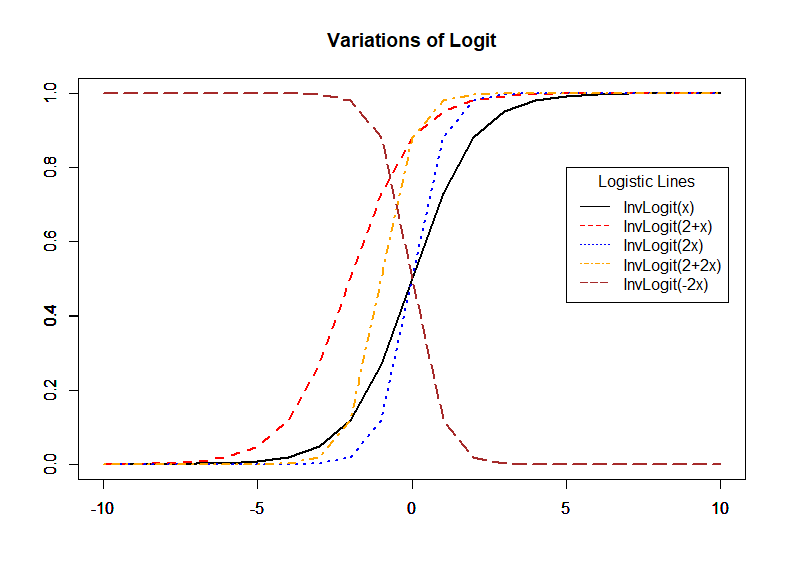
\includegraphics[scale=.5]{VarLogit}
\end{center}

\clearpage

Below is an example of a model logit and probit regressions, reconsidering our beer data as the only real ranking of beer is ``Very Good'' or ``Fair''; after all a ``Good'' ranking may not make sense to be any different from ``Fair.'' Rather, these two rankings are combined to make a zero-one variable (``very good'' versus ``good or fair'').

\begin{knitrout}
\definecolor{shadecolor}{rgb}{0.165, 0.169, 0.184}\color{fgcolor}\begin{kframe}
\begin{alltt}
\hlstd{> }\hlstd{logmod1} \hlkwb{<-} \hlkwd{glm}\hlstd{(beer_data}\hlopt{$}\hlstd{verygood} \hlopt{~} \hlstd{beer_data}\hlopt{$}\hlstd{price,}
\hlstd{+ }               \hlkwc{family} \hlstd{=} \hlkwd{binomial}\hlstd{(}\hlkwc{link}\hlstd{=logit))}
\hlstd{> }\hlcom{## summary(logmod1)  # Check your output}
\hlstd{> }
\hlstd{> }\hlstd{promod1} \hlkwb{<-} \hlkwd{glm}\hlstd{(beer_data}\hlopt{$}\hlstd{verygood} \hlopt{~} \hlstd{beer_data}\hlopt{$}\hlstd{price,}
\hlstd{+ }               \hlkwc{family} \hlstd{=} \hlkwd{binomial}\hlstd{(}\hlkwc{link}\hlstd{=probit))}
\hlstd{> }\hlcom{## summary(posmod1)}
\hlstd{> }
\hlstd{> }\hlcom{# Plot:   Using library(texreg)}
\hlstd{> }\hlkwd{texreg}\hlstd{(}\hlkwc{l}\hlstd{=} \hlkwd{list}\hlstd{(logmod1, promod1),} \hlkwc{stars} \hlstd{=} \hlkwd{numeric}\hlstd{(}\hlnum{0}\hlstd{),}
\hlstd{+ }       \hlkwc{custom.model.names} \hlstd{=} \hlkwd{c}\hlstd{(}\hlstr{"Logit Model"}\hlstd{,} \hlstr{"Probit Model"}\hlstd{),}
\hlstd{+ }       \hlkwc{custom.coef.names} \hlstd{=} \hlkwd{c}\hlstd{(}\hlstr{"Intercept"}\hlstd{,} \hlstr{"Price"}\hlstd{),}
\hlstd{+ }       \hlkwc{caption.above} \hlstd{= T,} \hlkwc{float.pos} \hlstd{=} \hlstr{"h!"}\hlstd{,}
\hlstd{+ }       \hlkwc{custom.note} \hlstd{=} \hlstr{"Dependent variable: Very Good Beer (1)"} \hlstd{)}
\end{alltt}
\end{kframe}
\end{knitrout}



\index{texreg package}
\begin{table}[h!]
\caption{Statistical models}
\begin{center}
\begin{tabular}{l c c }
\hline
 & Logit Model & Probit Model \\
\hline
Intercept      & $-3.12$  & $-1.96$  \\
               & $(1.29)$ & $(0.75)$ \\
Price          & $0.75$   & $0.48$   \\
               & $(0.40)$ & $(0.23)$ \\
\hline
AIC            & 42.96    & 42.79    \\
BIC            & 46.07    & 45.90    \\
Log Likelihood & -19.48   & -19.39   \\
Deviance       & 38.96    & 38.79    \\
Num. obs.      & 35       & 35       \\
\hline
\multicolumn{3}{l}{\scriptsize{Dependent variable: Very Good Beer (1)}}
\end{tabular}
\end{center}
\end{table}

From the table we see things to be very similar between the two models, the error reports (AIC, BIC, Log Likelihood, Deviance) are all similar, our price coefficient is still in the same sign, the logit model barely avoids significance whereas the probit model barely makes significance standards. Both coefficients are in the same direction however. Our intercepts vary between each other, but both are negative and significant.

Reading dichotomous outputs like these can be difficult, for the logit model a coeficient is the \textbf{changes in logged odds from moving from zero to a one}. Therefore, our price of .75 is the logged odds change from moving from a zero (a ``Fair or Good'' beer) to a ``Very Good'' beer (1). But we often don't think in terms of logged odds, therefore it is always helpful to calculate the multiplicative effect of each variable.

We can try to understand more about what makes ``Very Good'' beer by building a model one block at a time until we think we have a complete model for the data we have - guided by our theory about very good beer in this case.

\begin{knitrout}
\definecolor{shadecolor}{rgb}{0.165, 0.169, 0.184}\color{fgcolor}\begin{kframe}
\begin{alltt}
\hlstd{> }\hlcom{# Another texreg example: using library(texreg)}
\hlstd{> }\hlkwd{texreg}\hlstd{(}\hlkwc{l}\hlstd{=} \hlkwd{list}\hlstd{(logmod2, promod2),} \hlkwc{stars} \hlstd{=} \hlkwd{numeric}\hlstd{(}\hlnum{0}\hlstd{),}
\hlstd{+ }       \hlkwc{bold} \hlstd{= T,} \hlkwc{ci.force} \hlstd{= T,}   \hlcom{# Note some of these changes here}
\hlstd{+ }       \hlkwc{custom.model.names} \hlstd{=} \hlkwd{c}\hlstd{(}\hlstr{"Logit Model"}\hlstd{,} \hlstr{"Probit Model"}\hlstd{),}
\hlstd{+ }       \hlkwc{custom.coef.names} \hlstd{=} \hlkwd{c}\hlstd{(}\hlstr{"Intercept"}\hlstd{,} \hlstr{"Price"}\hlstd{,} \hlstr{"Availability"}\hlstd{,}
\hlstd{+ }                             \hlstr{"Alcohol Content"}\hlstd{,} \hlstr{"Caloric Content"}\hlstd{),}
\hlstd{+ }       \hlkwc{caption.above} \hlstd{= T,} \hlkwc{float.pos} \hlstd{=} \hlstr{"h!"}\hlstd{,}
\hlstd{+ }       \hlkwc{custom.note} \hlstd{=} \hlstr{"Dependent variable: Very Good Beer (1)"} \hlstd{)}
\end{alltt}
\end{kframe}
\end{knitrout}


\begin{table}[h!]
\caption{Statistical models}
\begin{center}
\begin{tabular}{l c c }
\hline
 & Logit Model & Probit Model \\
\hline
Intercept       & $\mathbf{-23.43}$ & $\mathbf{-14.03}$ \\
                & $[-43.03;\ -3.83]$    & $[-24.99;\ -3.07]$    \\
Price           & $1.11$                & $\mathbf{0.67}$   \\
                & $[-0.10;\ 2.33]$      & $[0.00;\ 1.33]$       \\
Availability    & $\mathbf{-3.53}$  & $\mathbf{-2.08}$  \\
                & $[-6.35;\ -0.71]$     & $[-3.63;\ -0.54]$     \\
Alcohol Content & $3.33$                & $1.94$                \\
                & $[-3.01;\ 9.67]$      & $[-1.59;\ 5.47]$      \\
Caloric Content & $0.04$                & $0.02$                \\
                & $[-0.10;\ 0.17]$      & $[-0.05;\ 0.10]$      \\
\hline
AIC             & 32.60                 & 32.20                 \\
BIC             & 40.37                 & 39.97                 \\
Log Likelihood  & -11.30                & -11.10                \\
Deviance        & 22.60                 & 22.20                 \\
Num. obs.       & 35                    & 35                    \\
\hline
\multicolumn{3}{l}{\scriptsize{Dependent variable: Very Good Beer (1)}}
\end{tabular}
\end{center}
\end{table}


The more specified table above includes the availability of the beer (is it often seen and promoted or more of an unknown beer to most bars), the alcohol, and caloric content; both of these are (at least chemically) to bring some form of pleasure and should be controlled. To switch up the data representation a little, confidence intervals are now shown and significance is indicated in bold.\footnote{ Texreg package customization, p.24 there is an example.} \index{texreg package}

Between the logit and probit models we still see a few differences, the intercept is again very different, likely because the difference in these models is the very distribution and link function they take which will shift the intercept; yet both are negative and significant. The price of the beer is insignificant for both models; yet, availability is significant for both models and in the negative direction (where 0 was a more frequent, popular beer). Alcohol and calorie levels are not significant for either model in predicting very good beers.\footnote{Interestingly caloric count is a low coefficient, likely because much of the variation is taken up by the alcohol content - which largely contributes to the calorie content in beer in the first place. An interaction between the two variables could be done, but this only inflates the alcohol content coefficient and all three variables become even further away from passing the significance threshold.} Finally, the model fitting reports are all very similar between the two models.

Going beyond sign and significance testing, let's first revisit our link function, if we take the inverse of the link function we can generate the ``mean function'' where instead of wrapping our link function around our linear predictor we can instead transform our DGP output itself. This can make more intuitive sense, and is again needed because then our values for $\eta$ will be from the zero to one interval.

\begin{equation}
\mathlarger{ \text{logit}^{-1} (\eta_i) = \frac{e^{\eta_i}}{1+e^{\eta_i}} \text{ to or from: } \eta_i = p\left( \frac{p}{1-p}\right) }
\end{equation}

Note from earlier that now in the logistic regression we are not dealing with a mere linear ``one unit in x causes an increase in y'' explanation. Rather, the logit regression is curved, and where we are at on the curve will determine how we read the regression coefficients. Generating predictive probabilities are always helpful, but require selecting a point of analysis per variable; this usually is set to the mean.

Consider our logit model from Table 4:

\begin{equation}
\mathlarger{ \text{logit}^{-1}(-23.43 + 1.11(\text{Price Value)} + \text{. . .} + 0.04(\text{Caloric Content))} }
\end{equation}

Here we could enter in mean numbers for each variable, and change the value we add per variable for interesting predicted probabilities in various scenarios that may be interesting to us. The number received is the probability of y happening given the parameters x given the data. This is both intuitive and interesting for readers.\footnote{Note this can also be done at the median of the data (intercept near zero), or at the middle category more generally. This is a case-by-case decision on whatever is most interesting given the question and data one is analyzing.}\index{``divide by four''}

The ``divide by four'' rule can be applied instead, were the beta coefficient is divided by four to yield the predictive probability \textit{at it's maximum in the middle of the curve}. At this point, directly in the middle (intercept = 0), the derivative of our function becomes equal to $\beta / 4$ allowing for an additional easy point estimate. Keep in mind this is best used for coefficients that are near the midpoint and not those on the tails because the logit distribution is much different at the tails than in the mid point. For example, in Table 4 our logit model showed the beer's availability had a large effect on the beer's rating. Taking it's availability $-3.53/4$ gives us a predictive probability of $-60.5$\%  That is, although this coefficient is away from the mean of the distribution, in example going from a widely available beer to a more sparse beer is likely to decrease the beer's rating (to the ``Good/Fair'' category) to a (approximate) 60.5\% probability.

Since it is usually better to represent these data in graphic form, consider a probability plot of our logistic curve for price now by the probability of receiving a very good beer:\footnote{The end section of this document, in quick overview, includes code for creating this.}


\begin{center}
\begin{knitrout}
\definecolor{shadecolor}{rgb}{0.165, 0.169, 0.184}\color{fgcolor}\begin{kframe}
\begin{alltt}
\hlstd{> }\hlkwd{library}\hlstd{(arm)} \hlcom{# for inverse logit function}
\hlstd{> }             \hlcom{# (It may actually be in the MASS package)}
\hlstd{> }
\hlstd{> }\hlcom{# Recall our logit model:}
\hlstd{> }\hlstd{logmod1} \hlkwb{<-} \hlkwd{glm}\hlstd{(verygood} \hlopt{~} \hlstd{price,} \hlkwc{data} \hlstd{= beer_data,}
\hlstd{+ }               \hlkwc{family} \hlstd{=} \hlkwd{binomial}\hlstd{(}\hlkwc{link}\hlstd{=logit))}
\hlstd{> }
\hlstd{> }\hlcom{# The inverse logit gets us our predicted probabilities:}
\hlstd{> }\hlcom{#   All we're doing here is using some base-R plotting operations}
\hlstd{> }\hlcom{#   with creating our predicted probabilities per our coefficents}
\hlstd{> }\hlkwd{curve}\hlstd{(}\hlkwd{invlogit}\hlstd{(logmod1}\hlopt{$}\hlstd{coef[}\hlnum{1}\hlstd{]} \hlopt{+} \hlstd{logmod1}\hlopt{$}\hlstd{coef[}\hlnum{2}\hlstd{]}\hlopt{*}\hlstd{x),} \hlnum{1}\hlstd{,} \hlnum{5}\hlstd{,} \hlkwc{ylim}\hlstd{=}\hlkwd{c}\hlstd{(}\hlopt{-}\hlnum{.01}\hlstd{,}\hlnum{.9}\hlstd{),}
\hlstd{+ }      \hlkwc{xlim}\hlstd{=}\hlkwd{c}\hlstd{(}\hlnum{0}\hlstd{,}\hlnum{7.5}\hlstd{),} \hlkwc{xaxt}\hlstd{=}\hlstr{"n"}\hlstd{,} \hlkwc{xaxs}\hlstd{=}\hlstr{"i"}\hlstd{,} \hlkwc{mgp}\hlstd{=}\hlkwd{c}\hlstd{(}\hlnum{2}\hlstd{,}\hlnum{.5}\hlstd{,}\hlnum{0}\hlstd{),}
\hlstd{+ }      \hlkwc{ylab}\hlstd{=}\hlstr{"Pr(Very Good Beer)"}\hlstd{,} \hlkwc{xlab}\hlstd{=}\hlstr{"Price"}\hlstd{,}
\hlstd{+ }      \hlkwc{main}\hlstd{=}\hlstr{"Probability of Very Good Beer, by Price"}\hlstd{,} \hlkwc{lwd}\hlstd{=}\hlnum{4}\hlstd{)}
\hlstd{> }\hlkwd{curve}\hlstd{(}\hlkwd{invlogit}\hlstd{(logmod1}\hlopt{$}\hlstd{coef[}\hlnum{1}\hlstd{]} \hlopt{+} \hlstd{logmod1}\hlopt{$}\hlstd{coef[}\hlnum{2}\hlstd{]}\hlopt{*}\hlstd{x),} \hlopt{-}\hlnum{2}\hlstd{,} \hlnum{8}\hlstd{,} \hlkwc{lwd}\hlstd{=}\hlnum{4.5}\hlstd{,} \hlkwc{add} \hlstd{= T)}
\hlstd{> }\hlkwd{axis}\hlstd{(}\hlnum{1}\hlstd{,} \hlnum{1}\hlopt{:}\hlnum{7}\hlstd{,} \hlkwc{mgp}\hlstd{=}\hlkwd{c}\hlstd{(}\hlnum{2}\hlstd{,}\hlnum{.5}\hlstd{,}\hlnum{0}\hlstd{))}
\hlstd{> }\hlkwd{mtext} \hlstd{(}\hlstr{"(two dollars)"}\hlstd{,} \hlnum{1}\hlstd{,} \hlnum{1.5}\hlstd{,} \hlkwc{at}\hlstd{=}\hlnum{2}\hlstd{,} \hlkwc{adj}\hlstd{=}\hlnum{.5}\hlstd{)} \hlcom{# just adding text to x axis}
\hlstd{> }\hlkwd{mtext} \hlstd{(}\hlstr{"(six dollars)"}\hlstd{,} \hlnum{1}\hlstd{,} \hlnum{1.5}\hlstd{,} \hlkwc{at}\hlstd{=}\hlnum{6}\hlstd{,} \hlkwc{adj}\hlstd{=}\hlnum{.5}\hlstd{)}
\hlstd{> }\hlkwd{points}\hlstd{(}\hlkwd{jitter}\hlstd{(beer_data}\hlopt{$}\hlstd{price,} \hlnum{1.5}\hlstd{),} \hlkwd{jitter}\hlstd{(beer_data}\hlopt{$}\hlstd{verygood,} \hlnum{0.1}\hlstd{),}
\hlstd{+ }       \hlkwc{pch}\hlstd{=}\hlnum{20}\hlstd{,} \hlkwc{cex}\hlstd{=}\hlnum{.9}\hlstd{)} \hlcom{# Jittered points so we can see them}
\end{alltt}
\end{kframe}
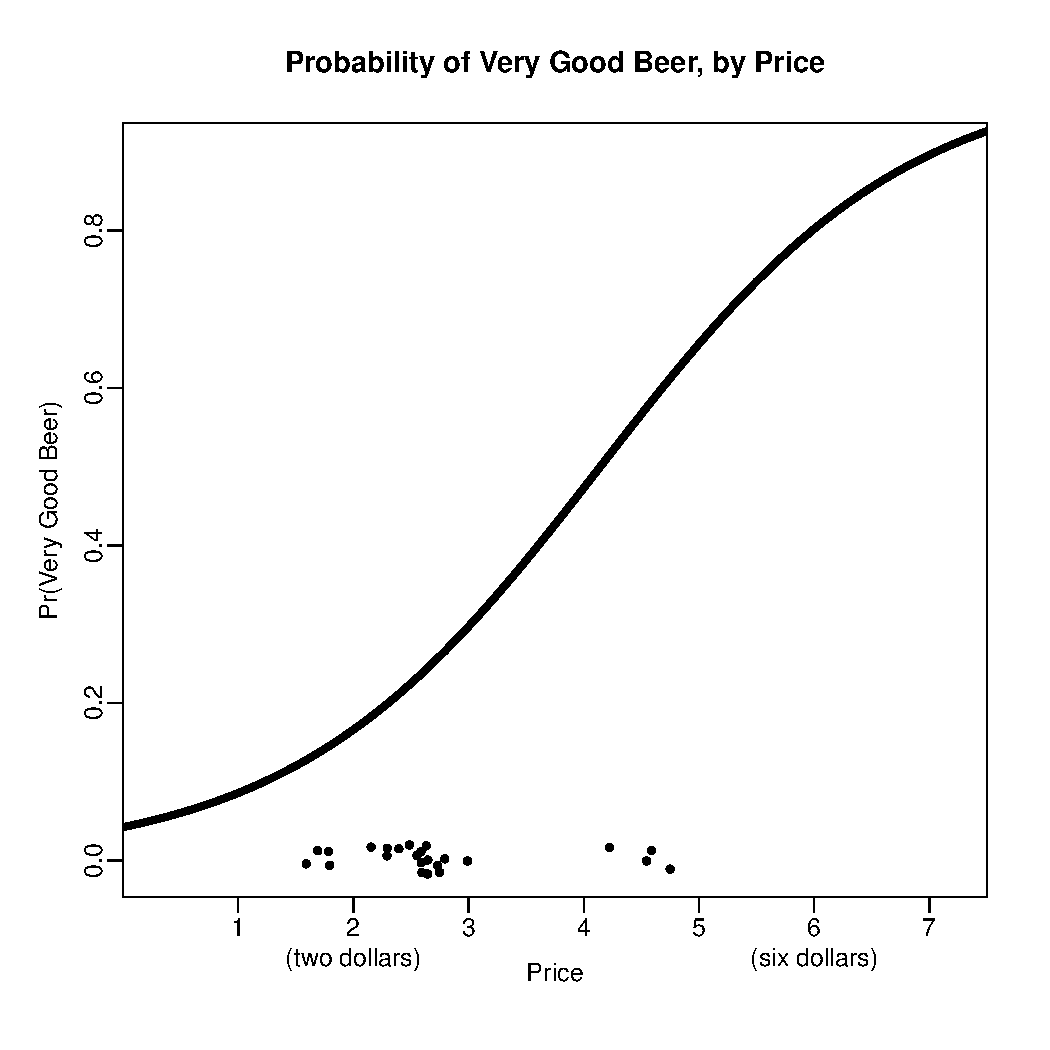
\includegraphics[width=5in]{figure/probplotlogit-1} 

\end{knitrout}
\end{center}


We can run some diagnostics on this similar to linear regression in that we're using residuals which are calculated similarly but for logit regression we have to ``bin'' these. I've done so for the initial model (only including price) and the full model (including calories and alcoholic content) below.\footnote{For more on why binned residual plotting: see Andrew Gelman (et. al's) article:\\ http://www.stat.columbia.edu/~gelman/research/published/dogs.pdf}

Here, ideally, we would want to see ``random noise'' around the dotted zero mark more average residuals. Additionally, we want about 95\% of the data to be encapsulated within the light grey lines. Thus, interpreting the graphs, we see a lot of data that stretches outside of the confidence bounds within both graphics. If one were to collect more data in the beer dataset we may be able to analyze this further, but as it is there seems to be not enough samples of very good beer to create a complete image of the ranking process in this dichotomous way. \index{Binned Residuals}

\begin{center}
\begin{knitrout}
\definecolor{shadecolor}{rgb}{0.165, 0.169, 0.184}\color{fgcolor}\begin{kframe}
\begin{alltt}
\hlstd{> }\hlkwd{library}\hlstd{(arm)}
\hlstd{> }
\hlstd{> }\hlcom{# Recall our logit models:}
\hlstd{> }\hlstd{logmod1} \hlkwb{<-} \hlkwd{glm}\hlstd{(verygood} \hlopt{~} \hlstd{price,} \hlkwc{data} \hlstd{= beer_data,}
\hlstd{+ }               \hlkwc{family} \hlstd{=} \hlkwd{binomial}\hlstd{(}\hlkwc{link}\hlstd{=logit))}
\hlstd{> }
\hlstd{> }\hlstd{logmod2} \hlkwb{<-} \hlkwd{glm}\hlstd{(verygood} \hlopt{~} \hlstd{price} \hlopt{+} \hlstd{avail} \hlopt{+} \hlstd{alcohol} \hlopt{+} \hlstd{calories,}
\hlstd{+ }               \hlkwc{data} \hlstd{= beer_data,}
\hlstd{+ }               \hlkwc{family} \hlstd{=} \hlkwd{binomial}\hlstd{(}\hlkwc{link}\hlstd{=logit))}
\hlstd{> }
\hlstd{> }\hlcom{## Binned Residual plotting ("arm" package)}
\hlstd{> }\hlkwd{par}\hlstd{(}\hlkwc{mfrow}\hlstd{=}\hlkwd{c}\hlstd{(}\hlnum{1}\hlstd{,}\hlnum{2}\hlstd{))}
\hlstd{> }\hlstd{x} \hlkwb{<-} \hlkwd{predict}\hlstd{(logmod1,} \hlkwc{type} \hlstd{=} \hlstr{"response"}\hlstd{)}
\hlstd{> }\hlstd{y} \hlkwb{<-} \hlkwd{resid}\hlstd{(logmod1)}
\hlstd{> }\hlkwd{binnedplot}\hlstd{(x, y,} \hlkwc{nclass}\hlstd{=}\hlkwa{NULL}\hlstd{,}
\hlstd{+ }           \hlkwc{xlab}\hlstd{=}\hlstr{"Expected Values"}\hlstd{,} \hlkwc{ylab}\hlstd{=}\hlstr{"Average residual"}\hlstd{,}
\hlstd{+ }           \hlkwc{main}\hlstd{=}\hlstr{"Binned residual plot: Model 1"}\hlstd{,}
\hlstd{+ }           \hlkwc{cex.pts}\hlstd{=}\hlnum{0.8}\hlstd{,} \hlkwc{col.pts}\hlstd{=}\hlnum{1}\hlstd{,} \hlkwc{col.int}\hlstd{=}\hlstr{"gray"}\hlstd{)}
\hlstd{> }
\hlstd{> }\hlcom{# Plot 2:}
\hlstd{> }\hlstd{x} \hlkwb{<-} \hlkwd{predict}\hlstd{(logmod2,} \hlkwc{type} \hlstd{=} \hlstr{"response"}\hlstd{)}
\hlstd{> }\hlstd{y} \hlkwb{<-} \hlkwd{resid}\hlstd{(logmod2)}
\hlstd{> }\hlkwd{binnedplot}\hlstd{(x, y,} \hlkwc{nclass}\hlstd{=}\hlkwa{NULL}\hlstd{,}
\hlstd{+ }           \hlkwc{xlab}\hlstd{=}\hlstr{"Expected Values"}\hlstd{,} \hlkwc{ylab}\hlstd{=}\hlstr{"Average residual"}\hlstd{,}
\hlstd{+ }           \hlkwc{main}\hlstd{=}\hlstr{"Binned residual plot: Model 2"}\hlstd{,}
\hlstd{+ }           \hlkwc{cex.pts}\hlstd{=}\hlnum{0.8}\hlstd{,} \hlkwc{col.pts}\hlstd{=}\hlnum{1}\hlstd{,} \hlkwc{col.int}\hlstd{=}\hlstr{"gray"}\hlstd{)}
\end{alltt}
\end{kframe}
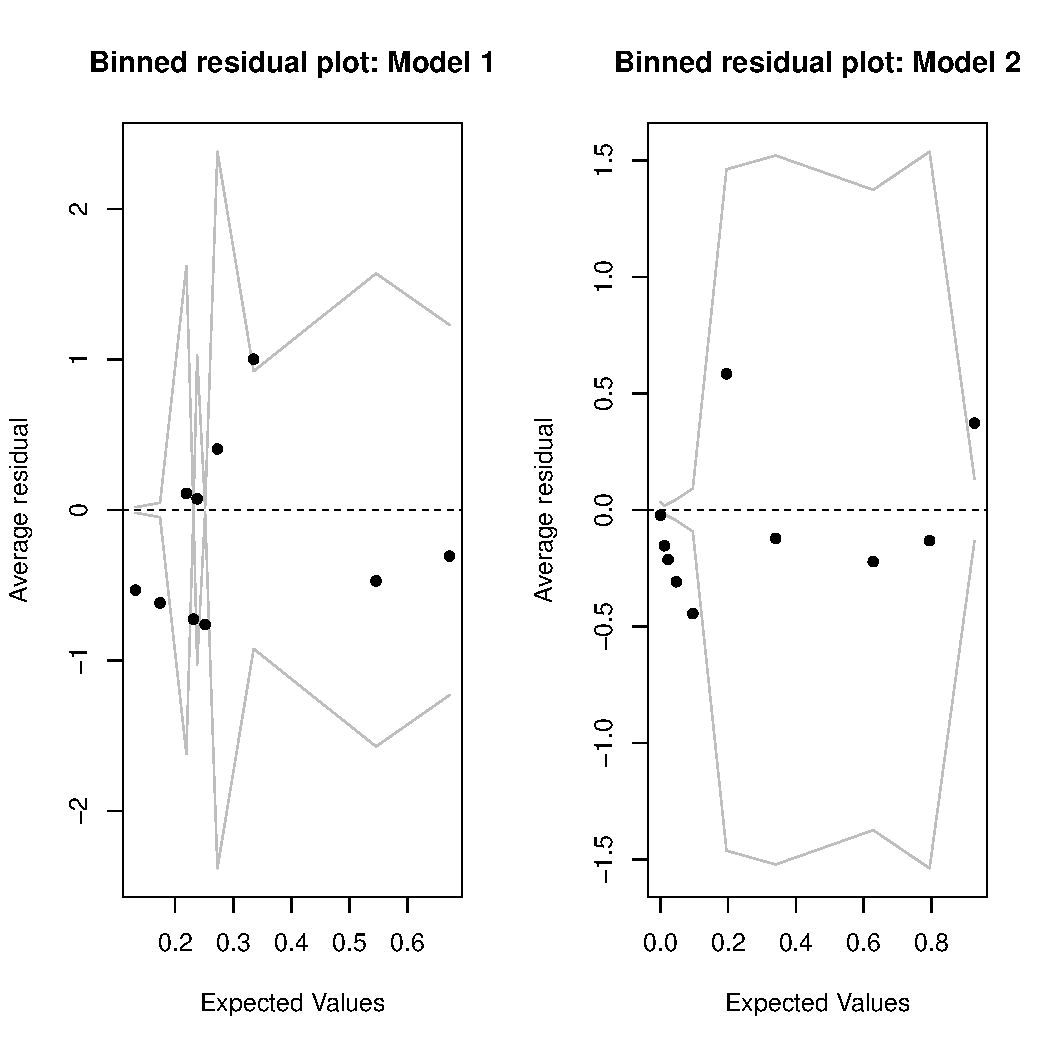
\includegraphics[width=5in,height=4.5in]{figure/binned-1} 
\begin{kframe}\begin{alltt}
\hlstd{> }\hlkwd{par}\hlstd{(}\hlkwc{mfrow}\hlstd{=}\hlkwd{c}\hlstd{(}\hlnum{1}\hlstd{,}\hlnum{1}\hlstd{))} \hlcom{# Reset graphing}
\end{alltt}
\end{kframe}
\end{knitrout}
\end{center}

%\begin{center}
%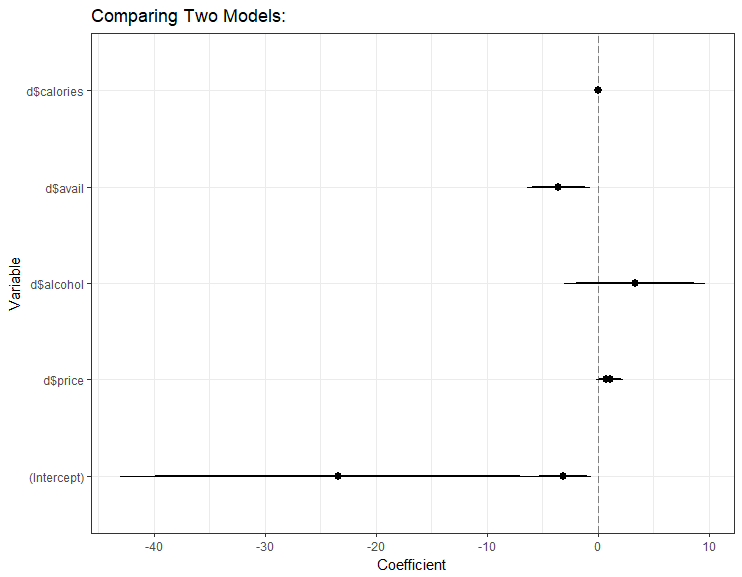
\includegraphics[scale=.7]{Rope}
%\end{center}

The below graphic compares the initial model with our full model in another great way, oftentimes readers prefer a visualization rather than tables. Our rope ladder plot shows just how little our two models differ, except in the wide-spread intercept, and few variables falling outside of the zero mark. Availability of the beer has a notable effect and is perhaps the main take away, along with price, of the logit models. High priced, widely available beer is very good in ranking (with some modeling concerns and error).
\index{Rope Ladder Ploting}

\begin{center}
\noindent\rule{8cm}{0.4pt}
\begin{knitrout}
\definecolor{shadecolor}{rgb}{0.165, 0.169, 0.184}\color{fgcolor}\begin{kframe}
\begin{alltt}
\hlstd{> }\hlkwd{library}\hlstd{(ggplot2)}
\hlstd{> }
\hlstd{> }\hlcom{# Rope Ladder Plot (ggplot2)}
\hlstd{> }\hlstd{f1}\hlkwb{<-}\hlkwd{data.frame}\hlstd{(}\hlkwc{Variable}\hlstd{=}\hlkwd{rownames}\hlstd{(}\hlkwd{summary}\hlstd{(logmod1)}\hlopt{$}\hlstd{coef),}
\hlstd{+ }               \hlkwc{Coefficient}\hlstd{=}\hlkwd{summary}\hlstd{(logmod1)}\hlopt{$}\hlstd{coef[,}\hlnum{1}\hlstd{],}
\hlstd{+ }               \hlkwc{SE}\hlstd{=}\hlkwd{summary}\hlstd{(logmod1)}\hlopt{$}\hlstd{coef[,}\hlnum{2}\hlstd{],}
\hlstd{+ }               \hlkwc{modelName}\hlstd{=} \hlstr{"Model 1"}\hlstd{)}
\hlstd{> }
\hlstd{> }\hlstd{f2}\hlkwb{<-}\hlkwd{data.frame}\hlstd{(}\hlkwc{Variable}\hlstd{=}\hlkwd{rownames}\hlstd{(}\hlkwd{summary}\hlstd{(logmod2)}\hlopt{$}\hlstd{coef),}
\hlstd{+ }               \hlkwc{Coefficient}\hlstd{=}\hlkwd{summary}\hlstd{(logmod2)}\hlopt{$}\hlstd{coef[,}\hlnum{1}\hlstd{],}
\hlstd{+ }               \hlkwc{SE}\hlstd{=}\hlkwd{summary}\hlstd{(logmod2)}\hlopt{$}\hlstd{coef[,}\hlnum{2}\hlstd{],}
\hlstd{+ }               \hlkwc{modelName}\hlstd{=} \hlstr{"Model 2"}\hlstd{)}
\hlstd{> }
\hlstd{> }\hlstd{combinedframe} \hlkwb{<-} \hlkwd{data.frame}\hlstd{(}\hlkwd{rbind}\hlstd{(f1, f2))}
\hlstd{> }\hlstd{interval1} \hlkwb{<-} \hlkwd{qnorm}\hlstd{((}\hlnum{1}\hlopt{-}\hlnum{0.9}\hlstd{)}\hlopt{/}\hlnum{2}\hlstd{)}
\hlstd{> }\hlstd{interval2} \hlkwb{<-} \hlkwd{qnorm}\hlstd{((}\hlnum{1}\hlopt{-}\hlnum{0.95}\hlstd{)}\hlopt{/}\hlnum{2}\hlstd{)}
\hlstd{> }
\hlstd{> }\hlstd{rl1} \hlkwb{<-} \hlkwd{ggplot}\hlstd{(combinedframe)}
\hlstd{> }\hlstd{rl1} \hlkwb{<-} \hlstd{rl1} \hlopt{+} \hlkwd{geom_hline}\hlstd{(}\hlkwc{yintercept} \hlstd{=} \hlnum{0}\hlstd{,} \hlkwc{color} \hlstd{=} \hlkwd{grey}\hlstd{(}\hlnum{1}\hlopt{/}\hlnum{2}\hlstd{),} \hlkwc{lty} \hlstd{=} \hlnum{5}\hlstd{)}
\hlstd{> }\hlstd{rl1} \hlkwb{<-} \hlstd{rl1} \hlopt{+} \hlkwd{geom_linerange}\hlstd{(}\hlkwd{aes}\hlstd{(}\hlkwc{x} \hlstd{= Variable,} \hlkwc{ymin} \hlstd{= Coefficient} \hlopt{-}
\hlstd{+ }\hlstd{SE}\hlopt{*}\hlstd{interval1,}
\hlstd{+ }               \hlkwc{ymax} \hlstd{= Coefficient} \hlopt{+} \hlstd{SE}\hlopt{*}\hlstd{interval1),}
\hlstd{+ }               \hlkwc{lwd} \hlstd{=} \hlnum{1}\hlstd{,} \hlkwc{position} \hlstd{=} \hlkwd{position_dodge}\hlstd{(}\hlkwc{width} \hlstd{=}\hlnum{1}\hlopt{/}\hlnum{2}\hlstd{))}
\hlstd{> }\hlstd{rl1} \hlkwb{<-} \hlstd{rl1} \hlopt{+} \hlkwd{geom_pointrange}\hlstd{(}\hlkwd{aes}\hlstd{(}\hlkwc{x} \hlstd{= Variable,} \hlkwc{y} \hlstd{= Coefficient,}
\hlstd{+ }\hlkwc{ymin} \hlstd{= Coefficient} \hlopt{-} \hlstd{SE}\hlopt{*}\hlstd{interval2,}
\hlstd{+ }               \hlkwc{ymax} \hlstd{= Coefficient} \hlopt{+} \hlstd{SE}\hlopt{*}\hlstd{interval2),}
\hlstd{+ }               \hlkwc{lwd} \hlstd{=} \hlnum{1}\hlopt{/}\hlnum{2}\hlstd{,} \hlkwc{position} \hlstd{=} \hlkwd{position_dodge}\hlstd{(}\hlkwc{width} \hlstd{=} \hlnum{1}\hlopt{/}\hlnum{2}\hlstd{),}
\hlstd{+ }               \hlkwc{color}\hlstd{=(}\hlstr{"Black"}\hlstd{),}
\hlstd{+ }               \hlkwc{shape} \hlstd{=} \hlnum{21}\hlstd{,} \hlkwc{fill} \hlstd{=} \hlstr{"BLACK"}\hlstd{)}
\hlstd{> }\hlstd{rl1} \hlkwb{<-} \hlstd{rl1} \hlopt{+} \hlkwd{coord_flip}\hlstd{()} \hlopt{+} \hlkwd{theme_bw}\hlstd{()}
\hlstd{> }\hlstd{rl1} \hlkwb{<-} \hlstd{rl1} \hlopt{+} \hlkwd{ggtitle}\hlstd{(}\hlstr{"Comparing Two Models:"}\hlstd{)}
\hlstd{> }\hlkwd{print}\hlstd{(rl1)}
\end{alltt}
\end{kframe}
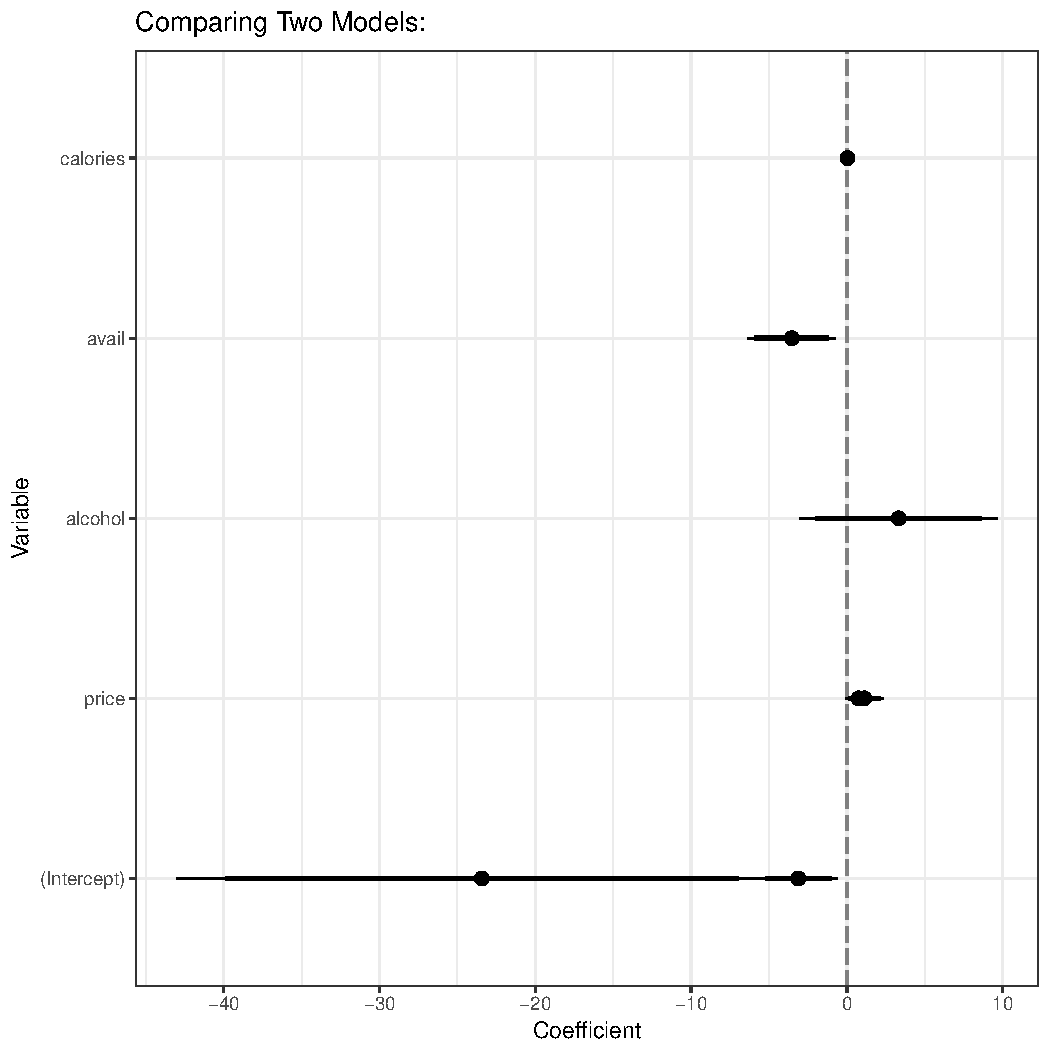
\includegraphics[width=5in,height=5in]{figure/rope-1} 

\end{knitrout}
\end{center}







%----------







\clearpage
\subsection{Poisson Modeling:}
Poisson data uses a new link function which allows us to model count-level data, the probability mass function (pmf) now being:

\begin{equation}
\mathlarger{ \frac{\lambda^k e^{-\lambda}}{k!}     }
\end{equation}

Where the available numbers the model will take are all real numbers greater than zero $(0; 1; 2; 3; 4; 5; ...)$. This normal Poisson model assumes the variance is equal to it's mean, but often we see the variance to be greater (over-dispersed) or lower (under-dispersed) than the mean. This assumption is oftentimes broken in social sciences, for this reason a \textit{quasi-Poisson} or \textit{negative binomial} is able to let the variance change.
\begin{equation}
\text{Quasi-Poisson:} \hspace{.3cm} var(Y)=\theta \mu \hspace{.3cm}\text{Where theta is the overdispersion parameter}
\end{equation}
\begin{equation}
 \text{Negative Binomial:} \hspace{.3cm} var(Y)= \mu (1+ K\mu) \hspace{.3cm} \text{Where K is the shape parameter}
\end{equation}
How we handle the differences between the variance and mean relations in each of these three forms of count-data modeling may effect our regression coefficients fit differences between negative binomial (also known as gamma-Poisson), quasi-Poisson, and regular Poisson modeling. This is because fitting these models uses weighted least squares, and these weights are inversely proportional to the variance. Thus, negative binomial and quasi-Poisson will weight observations differently. Ultimately, the decision to choose the quasi-Poisson or another variation the negative binomial regression should depend on the theory rather than the data-driven method.\footnote{Ver Hoef, Jay M. and Boveng, Peter L., "QUASI-POISSON VS. NEGATIVE BINOMIAL REGRESSION: HOW SHOULD WE
MODEL OVERDISPERSED COUNT DATA?" (2007). Publications, Agencies and Staff of the U.S. Department of Commerce. Paper
142.}

Let's build a regular Poisson model, adding one variable at a time, to predict the likelihood of a successful military coup (R's faraway package). Let's assume that we theorize that the percent of a country voting, the years of oligarchy, number of elections, and political liberalization all make sense towards predicting the number (count) of successful military coups. Results are shown in Table 5 below, however here is how these models are ran in R:

\begin{knitrout}
\definecolor{shadecolor}{rgb}{0.165, 0.169, 0.184}\color{fgcolor}\begin{kframe}
\begin{alltt}
\hlstd{> }\hlkwd{library}\hlstd{(faraway)}
\end{alltt}


{\ttfamily\noindent\color{warningcolor}{\#\# Warning: package 'faraway' was built under R version 3.3.3}}\begin{alltt}
\hlstd{> }\hlkwd{library}\hlstd{(MASS)}
\hlstd{> }\hlkwd{data}\hlstd{(africa)}
\hlstd{> }
\hlstd{> }\hlcom{## Examine Dataset ##}
\hlstd{> }\hlkwd{str}\hlstd{(africa)}  \hlcom{# There are some NAs in the data to consider}
\end{alltt}
\begin{verbatim}
## 'data.frame':	47 obs. of  9 variables:
##  $ miltcoup : int  0 5 0 6 2 0 1 3 1 2 ...
##  $ oligarchy: int  0 7 0 13 13 0 0 14 15 0 ...
##  $ pollib   : int  2 1 NA 2 2 2 2 2 2 2 ...
##  $ parties  : int  38 34 7 62 10 34 5 14 27 4 ...
##  $ pctvote  : num  NA 45.7 20.3 17.5 34.4 ...
##  $ popn     : num  9.7 4.6 1.2 8.8 5.3 11.6 0.361 3 5.5 0.458 ...
##  $ size     : num  1247 113 582 274 28 ...
##  $ numelec  : int  0 8 5 5 3 14 2 6 4 6 ...
##  $ numregim : int  1 3 1 3 3 3 1 4 3 2 ...
\end{verbatim}
\begin{alltt}
\hlstd{> }\hlcom{# Poisson}
\hlstd{> }\hlstd{mod4} \hlkwb{<-} \hlkwd{glm}\hlstd{(africa}\hlopt{$}\hlstd{miltcoup} \hlopt{~} \hlstd{africa}\hlopt{$}\hlstd{pctvote} \hlopt{+} \hlstd{africa}\hlopt{$}\hlstd{oligarchy} \hlopt{+}
\hlstd{+ } \hlstd{africa}\hlopt{$}\hlstd{numelec} \hlopt{+} \hlstd{africa}\hlopt{$}\hlstd{pollib,} \hlkwc{family} \hlstd{= poisson)}
\hlstd{> }
\hlstd{> }\hlcom{# Quasi Poisson}
\hlstd{> }\hlstd{qmod4} \hlkwb{<-} \hlkwd{glm}\hlstd{(africa}\hlopt{$}\hlstd{miltcoup} \hlopt{~} \hlstd{africa}\hlopt{$}\hlstd{pctvote} \hlopt{+} \hlstd{africa}\hlopt{$}\hlstd{oligarchy} \hlopt{+}
\hlstd{+ } \hlstd{africa}\hlopt{$}\hlstd{numelec} \hlopt{+} \hlstd{africa}\hlopt{$}\hlstd{pollib,} \hlkwc{family} \hlstd{= quasipoisson)}
\end{alltt}
\end{kframe}
\end{knitrout}



\hfill \\
\noindent \textbf{More on Dispersion Problems:}\\
In the Poisson distribution we make a rather strong assumption that our mean is equal to the variance due to the Poisson link function only having one parameter. We rarely ever fulfill this assumption in social sciences, but are able to report and correct for our dispersion problems pretty well. If our model is \textit{over-dispersed} this means that our mean is a certain distribution with a peak and the variance is larger than that actual mean distribution (not being equal as our assumption posits). The inverse is defined as under-dispersion although this is less common. A few ways to control for dispersion would be to check the F-statistic to report model-fit more accurately per variable as we're building our model. Also, we can check the typical robustness checks from the linear model including the QQ plot, Cook's Distance, and residual plotting. It may be the case that a logarithmic transformation (or similar transformation) of a variable will better-fit our model without actually changing and values given that they are all scaled together. Note how the regular Poisson assumption is a special case of the Quasi-Poisson regression (where $\theta$ equals one we arrive at the Poisson assumption $var(Y)=1\mu$. Often using Quasi-Poisson regression isn't a bad idea considering we rarely fulfill the Poisson dispersion assumption.\\

\begin{table}[h!]
\caption{Statistical models}
\begin{center}
\begin{tabular}{l c c c c }
\hline
 & Model 1 & Model 2 & Model 3 & Model 4 \\
\hline
Intercept                & $0.29$   & $-0.52$  & $-1.34$  & $-0.17$  \\
                         & $(0.28)$ & $(0.37)$ & $(0.61)$ & $(0.73)$ \\
Percent Voting           & $0.00$   & $0.00$   & $0.00$   & $0.00$   \\
                         & $(0.01)$ & $(0.01)$ & $(0.01)$ & $(0.01)$ \\
Years of Oligarchy       &          & $0.11$   & $0.13$   & $0.11$   \\
                         &          & $(0.02)$ & $(0.02)$ & $(0.02)$ \\
Number of Elections      &          &          & $0.10$   & $0.05$   \\
                         &          &          & $(0.05)$ & $(0.06)$ \\
Political Liberalization &          &          &          & $-0.40$  \\
                         &          &          &          & $(0.24)$ \\
\hline
AIC                      & 149.55   & 120.73   & 118.61   & 111.67   \\
BIC                      & 152.98   & 125.87   & 125.47   & 119.59   \\
Log Likelihood           & -72.77   & -57.36   & -55.31   & -50.83   \\
Deviance                 & 80.74    & 49.92    & 45.80    & 36.86    \\
Num. obs.                & 41       & 41       & 41       & 36       \\
\hline
\multicolumn{5}{l}{\scriptsize{Dependent variable: Successful Military Coups}}
\end{tabular}
\end{center}
\end{table}

We can include and check the chi-squared of our model since it is compatible to our Poisson distribution:\\
\begin{equation}
\mathlarger{ \hat{\phi} = \frac{\chi^2}{n-p} = \frac{\Sigma_i(y_i - \hat{\lambda_i})^2 /\hat{ \lambda_i}}{n-p} }
\end{equation}
More easily computed in R:\\

\begin{knitrout}
\definecolor{shadecolor}{rgb}{0.165, 0.169, 0.184}\color{fgcolor}\begin{kframe}
\begin{alltt}
\hlstd{> }\hlcom{# ChiSquared of Model 4}
\hlstd{> }\hlstd{dp} \hlkwb{<-} \hlkwd{sum}\hlstd{(}\hlkwd{residuals}\hlstd{(mod4,} \hlkwc{type}\hlstd{=}\hlstr{"pearson"}\hlstd{)}\hlopt{^}\hlnum{2}\hlstd{)}\hlopt{/}\hlstd{mod4}\hlopt{$}\hlstd{df.residual}
\hlstd{> }\hlstd{dp}
\end{alltt}
\begin{verbatim}
## [1] 1.155917
\end{verbatim}
\end{kframe}
\end{knitrout}

We can just run a quasi-Poisson family regression to get similar results initially. The follow is the two models comparatively:

\clearpage


\begin{table}[h!]
\caption{Statistical models}
\begin{center}
\begin{tabular}{l c c }
\hline
 & Q-Model 4 & Model 4 \\
\hline
Intercept                & $-0.17$  & $-0.17$  \\
                         & $(0.78)$ & $(0.73)$ \\
Percent Voting           & $0.00$   & $0.00$   \\
                         & $(0.01)$ & $(0.01)$ \\
Years of Oligarchy       & $0.11$   & $0.11$   \\
                         & $(0.03)$ & $(0.02)$ \\
Number of Elections      & $0.05$   & $0.05$   \\
                         & $(0.06)$ & $(0.06)$ \\
Political Liberalization & $-0.40$  & $-0.40$  \\
                         & $(0.25)$ & $(0.24)$ \\
\hline
AIC                      &          & 111.67   \\
BIC                      &          & 119.59   \\
Log Likelihood           &          & -50.83   \\
Deviance                 & 36.86    & 36.86    \\
Num. obs.                & 36       & 36       \\
\hline
\multicolumn{3}{l}{\scriptsize{Dependent variable: Successful Military Coups}}
\end{tabular}
\end{center}
\end{table}

Notice that the coefficients don't change much at all, but reconsidering our measure of the variance has changed some significance levels slightly. Note we cannot see our AIC, BIC, or Log Likelihood for the quasi-Poisson; this is because of how the variance is manipulated, a Quasi-AIC measure would be needed to report that finding. Also, we could include a negative binomial model next to the others:

\begin{knitrout}
\definecolor{shadecolor}{rgb}{0.165, 0.169, 0.184}\color{fgcolor}\begin{kframe}
\begin{alltt}
\hlstd{> }\hlcom{# Poisson}
\hlstd{> }\hlstd{mod4} \hlkwb{<-} \hlkwd{glm}\hlstd{(africa}\hlopt{$}\hlstd{miltcoup} \hlopt{~} \hlstd{africa}\hlopt{$}\hlstd{pctvote} \hlopt{+} \hlstd{africa}\hlopt{$}\hlstd{oligarchy} \hlopt{+}
\hlstd{+ } \hlstd{africa}\hlopt{$}\hlstd{numelec} \hlopt{+} \hlstd{africa}\hlopt{$}\hlstd{pollib,} \hlkwc{family} \hlstd{= poisson)}
\hlstd{> }
\hlstd{> }\hlcom{# Quasi Poisson}
\hlstd{> }\hlstd{qmod4} \hlkwb{<-} \hlkwd{glm}\hlstd{(africa}\hlopt{$}\hlstd{miltcoup} \hlopt{~} \hlstd{africa}\hlopt{$}\hlstd{pctvote} \hlopt{+} \hlstd{africa}\hlopt{$}\hlstd{oligarchy} \hlopt{+}
\hlstd{+ } \hlstd{africa}\hlopt{$}\hlstd{numelec} \hlopt{+} \hlstd{africa}\hlopt{$}\hlstd{pollib,} \hlkwc{family} \hlstd{= quasipoisson)}
\hlstd{> }
\hlstd{> }\hlcom{# Negative Binomial}
\hlstd{> }\hlstd{nbmod4} \hlkwb{<-} \hlkwd{glm.nb}\hlstd{(africa}\hlopt{$}\hlstd{miltcoup} \hlopt{~} \hlstd{africa}\hlopt{$}\hlstd{pctvote} \hlopt{+} \hlstd{africa}\hlopt{$}\hlstd{oligarchy} \hlopt{+}
\hlstd{+ } \hlstd{africa}\hlopt{$}\hlstd{numelec} \hlopt{+} \hlstd{africa}\hlopt{$}\hlstd{pollib)}
\end{alltt}
\end{kframe}
\end{knitrout}

\clearpage

\begin{table}[h!]
\caption{Statistical models}
\begin{center}
\begin{tabular}{l c c c }
\hline
 & Model 4 & Q-Model 4 & Negative-Binomial Model 4 \\
\hline
Intercept                & $-0.17$  & $-0.17$  & $-0.17$  \\
                         & $(0.73)$ & $(0.78)$ & $(0.73)$ \\
Percent Voting           & $0.00$   & $0.00$   & $0.00$   \\
                         & $(0.01)$ & $(0.01)$ & $(0.01)$ \\
Years of Oligarchy       & $0.11$   & $0.11$   & $0.11$   \\
                         & $(0.02)$ & $(0.03)$ & $(0.02)$ \\
Number of Elections      & $0.05$   & $0.05$   & $0.05$   \\
                         & $(0.06)$ & $(0.06)$ & $(0.06)$ \\
Political Liberalization & $-0.40$  & $-0.40$  & $-0.40$  \\
                         & $(0.24)$ & $(0.25)$ & $(0.24)$ \\
\hline
AIC                      & 111.67   &          & 113.67   \\
BIC                      & 119.59   &          & 123.17   \\
Log Likelihood           & -50.83   &          & -50.83   \\
Deviance                 & 36.86    & 36.86    & 36.85    \\
Num. obs.                & 36       & 36       & 36       \\
\hline
\multicolumn{4}{l}{\scriptsize{Dependent variable: Successful Military Coups}}
\end{tabular}
\end{center}
\end{table}


Ultimately, for publication I would include all of these in an appendix or supplemental appendix. Our results themselves are largely insignificant and our coefficients, using $\mathlarger{ e^{\beta} }$ we can find the multiplicative change of each variable's coefficient. The most significant finding (consistently) is the years of oligarchy a country experiences predicts the multiplicative likelihood of a military coup. For interpretation, our $\beta = .11$ so $e^{.11} = 1.116278$ or an 12\% increase in the likelihood of a military coup as years of oligarchy increases. In Table 8 I do what is most intuitive for readers, report a model (in this case the negative binomial) and it's associated percentage likelihood estimate.
\clearpage


\begin{table}[h!]
\caption{Statistical models}
\begin{center}
\begin{tabular}{l c c }
\hline
 & Negative-Binomial Model & $1- e^\beta$  \\
\hline
Intercept                 & $-0.17$    & \\
                          & $(0.73)$   & \\
Percent Voting            & $0.00$     & $0\%$ \\
                          & $(0.01)$   &\\
Years of Oligarchy        & $0.11$     & $12\%$ \\
                          & $(0.02)$   &\\
Number of Elections       & $0.05$     & $5\% $ \\
                          & $(0.06)$   &\\
Political Liberalization  & $-0.40$    & $-33\%$\\
                          & $(0.24)$   &\\
\hline
AIC                       & 113.67     &\\
BIC                       & 123.17     &\\
Log Likelihood            & -50.83     &\\
Deviance                  & 36.85      &\\
Num. obs.                 & 36         & 36\\
\hline
\multicolumn{3}{l}{\scriptsize{Dependent variable: Successful Military Coups}}
\end{tabular}
\end{center}
\end{table}


%--------------------------------------------------------------------------------------------
\addcontentsline{toc}{subsubsection}{Likelihood Ratio Test, Deviance, AIC, and BIC}
\noindent \textbf{Likelihood Ratio Test, Deviance, AIC, and BIC:}\\
In the likelihood ratio test we have two models where one is a subset (or nested) within another (following is using hypothetical data). Here we have the likelihoods of both of the restricted model ($\hat{L_R}$) divided by the unrestricted model ($\hat{L_U}$) thus taking their ratio. Using hypothetical data our restricted model logged-likelihood is -469.174 and our unrestricted model is a logged-likelihood of -406.0718. So assume here we have a restricted model with a higher logged-likelihood than the unrestricted model which isn't ideal of a likelihood ratio test. Further, our logged-likelihoods are negative which is also not ideal in creating an interpret-able likelihood ratio test. Exponentiating each of these:\\
\begin{equation}
\mathlarger{ \lambda = \frac{ \hat{L_R}}{ \hat{L_U}} = \frac{ e^{-469.174}}{e^{-406.0718}} = 3.9360695\text{e}-28 }
\end{equation}

Given that this doesn't really work, and our results would be helpful but we would have to just interpret arbitrary an arbitrary ``cut-off" point between zero and one to determine if we can reject the null or not, we can actually just use a \textbf{logged-likelihood ratio test} which is similar but not exactly a likelihood ratio (although this is more common):\\
\begin{equation}
\mathlarger{  \lambda = -2 \ln \left( \frac{ \hat{L_R}}{ \hat{L_U}}  \right) = -2 \left[(-469.174) - (-406.0718) \right] = 126.2044  }
\end{equation}

\clearpage

We could run this number in R: \\

\begin{knitrout}
\definecolor{shadecolor}{rgb}{0.165, 0.169, 0.184}\color{fgcolor}\begin{kframe}
\begin{alltt}
\hlstd{> }\hlkwd{dchisq}\hlstd{(}\hlnum{126.2044}\hlstd{,} \hlkwc{df}\hlstd{=}\hlnum{1}\hlstd{)}
\end{alltt}
\begin{verbatim}
## [1] 1.39777e-29
\end{verbatim}
\end{kframe}
\end{knitrout}


Similarly we can calculate the deviance, or the difference between a perfect fitting model and our models. Given that a perfect fitting model (for general linear models at least) are by definition perfect, the math becomes easier because perfect models can be understood as zero: \\
\begin{equation}
D = 2(0- \ln L(\hat{\theta} \vert y)
\end{equation}
\begin{equation}
 D = -2( \ln L(\hat{\theta} \vert y)
\end{equation}
Although the calculation doesn't involve pitting the models against each other we can compare model's distance away from the ideal models. We can also look at the AIC and BIC, defined similarly:\\
\begin{equation}
AIC = -2 \ln L(\hat{\theta} \vert y) + 2p = D(\hat{\theta} ) +2p
\end{equation}
\begin{equation}
BIC = -2 \ln L(\hat{\theta} \vert x) +plog(n) = D(\hat{\theta}) + p \ln (n)
\end{equation}


These are important to apply because if we arbitrarily add more and more variables into a model, our deviance will continue to decrease although this may not be honest to our actual understand of a ``better'' model (kitchen-sink models). AIC adds $2p$ where p is the number of parameters; thus, this adds a linear check against our deviance. BIC adds $p\cdot log(n)$ or a non-linear check on our deviance. Together than can help us check our model fit (and is often automatically calculated for you in tables in R) \\

Overall, the AIC, BIC, Log Likelihood, and Deviance are all great indicators for model fit from the ideal model and checking for many parameters (both linearly and non-linearly).

















\clearpage
\subsection{Ordered Logistic Modeling:}

Ordered models take data that has a scale in responses, where a ``1'' response is less than or greater than a ``2'' response which is in similar direction to a ``3'' response. These ordered responses, in order to work in a GLM framework, must be formulated to be measurable at each disjointed segment between each ordered response. It may be helpful to think of this as a series of logitstic regressions between the segments, in the end bonded together. Therefore, we get the link function for the ordered logistic:\\ \index{link function}
\begin{equation}
\mathlarger{ \frac{1}{1+ e^{-(\theta_i- w\cdot x)}   }  }
\end{equation}
\noindent and (optionally) the ordered probit could be used, or a sometimes attractive third option which is the exponential function to create a proportional hazards model, although survival models will be covered at the end of this document these two models are relatives of one another:\\
\begin{equation}
exp(-exp(\theta_i - w \cdot x))
\end{equation}
Intuitively, with a series of logistic regressions we could subtract these categories to find the effects of each category; or add these categories up to equal 1. If these categories do not add up to one the remaining number is the coefficient for a left out category. Subtracting these categories requires subtracting the inverse logit of each: $logit^{-1}(\theta_{k+1}) - logit^{-1} (\theta_k)$. AIC and BIC, note, will be including all disjointed segments. Also, by doing a regression we are not finding the areas between these ``cut points" but rather the label (or response) at each cut point itself. We can take the derivative of the line estimate between cut points to find the nuanced area in between cut points, but subtracting the inverse logits (above) is essentially the same result.

Revising the data on beer, we should realize that our ranking variable is directly suited for ordered logistic regression (not OLS). Let's see if our findings differ in any way from the OLS or logit models we ran. Consider an ordinal logit of the beer ranking:



\begin{table}[h!]
\caption{Statistical models}
\begin{center}
\begin{tabular}{l c c }
\hline
 & Model 1 & Model 2 \\
\hline
Price           & $0.74$   & $0.63$   \\
                & $(0.36)$ & $(0.36)$ \\
Alcohol Content &          & $1.75$   \\
                &          & $(0.82)$ \\
\hline
AIC             & 76.76    & 72.04    \\
BIC             & 81.42    & 78.27    \\
Log Likelihood  & -35.38   & -32.02   \\
Deviance        & 70.76    & 64.04    \\
Num. obs.       & 35       & 35       \\
\hline
\multicolumn{3}{l}{\scriptsize{Dependent variable: Quality of Beer Ranking}}
\end{tabular}
\end{center}
\end{table}



Interpretation of the results are similar to logit regression in that they are the logged odds change from one cut point to another cut point. That is, from a ``2'' quality to a ``3'' we see a 1.75 logged percentage increase per unit increase in alcohol content. This effect is statistically significant.

\addcontentsline{toc}{subsubsection}{Bootstrapping}
\hfill \\
\noindent \textbf{Bootstrapping:}

One issue to consider is the low observation number (N) but high demand of the model (varying categorical demands of our dependent variable). One robustness check of this is to \textit{bootstrap} the model to use simulation to build up the number of observations to fulfill our assumption of normal distribution which may be a hard assumption without doing this:
\begin{center}
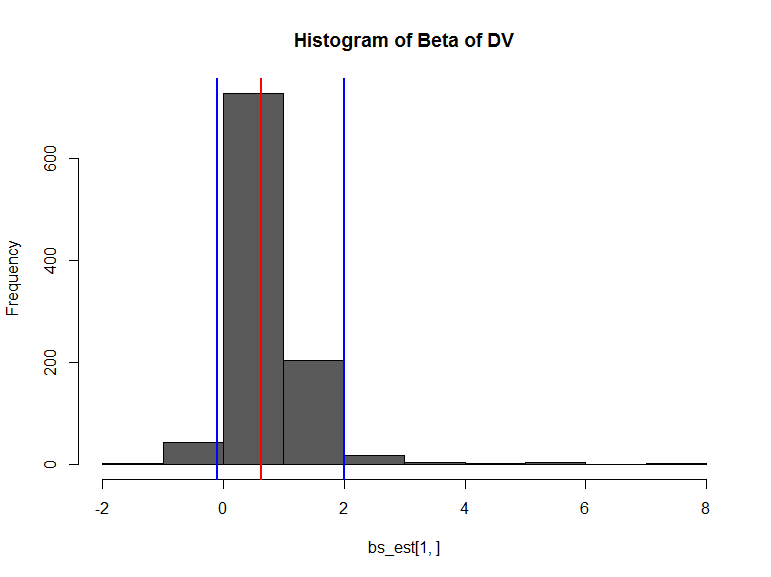
\includegraphics[scale=.65]{best}
\end{center}
Above, we see our beta estimate is not a very good normal distribution even though our model assumptions assume that we should treat it like one. In order to make the assumption of normal distribution we can bootstrap the model by replicating it's draws. Figure 2 maps a normal distribution and marks the same model's beta coefficients information to show an ideal model:

\clearpage

\begin{center}
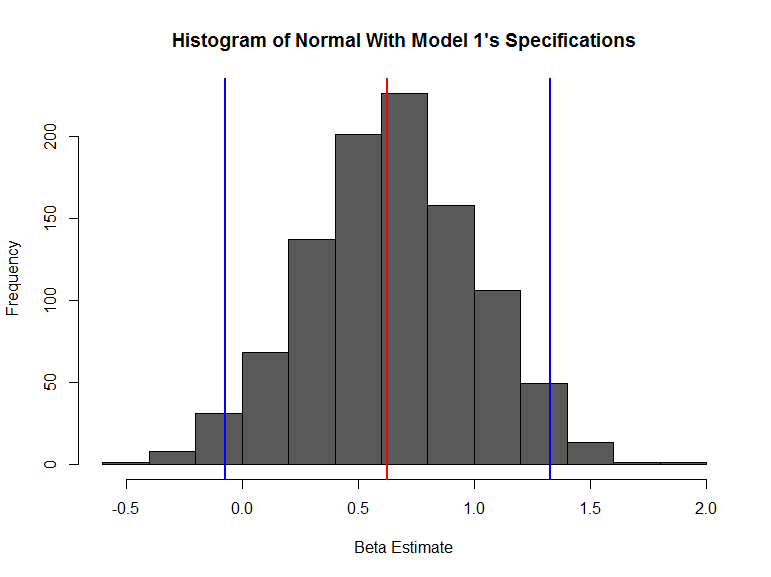
\includegraphics[scale=.6]{Nbest}
\end{center}

Using these new-found thresholds, including a red mean line ideally where it should between the blue lower and upper bounds, we can re-run our model based upon the new information - creating new high and low confidence intervals, we find that significance still remains in Table 10: \\

\begin{table}[h!]
\caption{Statistical models}
\begin{center}
\begin{tabular}{l c }
\hline
 & Model 1 \\
\hline
Price           & $0.63$           \\
                & $[-0.08;\ 1.95]$ \\
Alcohol Content & $1.75^{*}$       \\
                & $[0.62;\ 4.96]$  \\
\hline
AIC             & 72.04            \\
BIC             & 78.27            \\
Log Likelihood  & -32.02           \\
Deviance        & 64.04            \\
Num. obs.       & 35               \\
\hline
\multicolumn{2}{l}{\scriptsize{Dependent variable: Quality of Beer Ranking}}
\end{tabular}
\end{center}
\end{table}


This will typically yield more conservative estimations and evaluations of our standard errors, commonly in cases with low N. Code for this process:

\begin{knitrout}
\definecolor{shadecolor}{rgb}{0.165, 0.169, 0.184}\color{fgcolor}\begin{kframe}
\begin{alltt}
\hlstd{> }\hlkwd{set.seed}\hlstd{(}\hlnum{10}\hlstd{)}
\hlstd{> }\hlcom{# This seed is used, it assures replication and convergence for this model}
\hlstd{> }
\hlstd{> }\hlcom{# For Bootstrapping:}
\hlstd{> }\hlstd{bs.sample} \hlkwb{<-} \hlkwa{function}\hlstd{(}\hlkwc{dat}\hlstd{)}
\hlstd{+ }\hlstd{\{}
\hlstd{+ }  \hlstd{idx} \hlkwb{<-} \hlkwd{sample}\hlstd{(}\hlnum{1}\hlopt{:}\hlkwd{nrow}\hlstd{(dat),} \hlkwd{nrow}\hlstd{(dat),} \hlkwc{replace} \hlstd{=} \hlnum{TRUE}\hlstd{)}
\hlstd{+ }  \hlstd{dat[idx,]}
\hlstd{+ }\hlstd{\}}
\hlstd{> }
\hlstd{> }\hlstd{bs.routine} \hlkwb{<-} \hlkwa{function}\hlstd{(}\hlkwc{dat}\hlstd{)}
\hlstd{+ }\hlstd{\{}
\hlstd{+ }  \hlstd{sample.dta} \hlkwb{<-} \hlkwd{bs.sample}\hlstd{(dat)}
\hlstd{+ }  \hlkwd{coef}\hlstd{(MASS}\hlopt{::}\hlkwd{polr}\hlstd{(}\hlkwd{as.factor}\hlstd{(quality)} \hlopt{~} \hlstd{price} \hlopt{+} \hlstd{alcohol,}
\hlstd{+ }                  \hlkwc{data} \hlstd{= sample.dta))}
\hlstd{+ }\hlstd{\}}
\hlstd{> }\hlstd{bs_est} \hlkwb{<-} \hlkwd{replicate}\hlstd{(}\hlnum{1000}\hlstd{,} \hlkwd{bs.routine}\hlstd{(}\hlkwc{dat} \hlstd{= beer_data))}
\hlstd{> }\hlcom{# replicate is actually doing the bootstrap^}
\hlstd{> }
\hlstd{> }\hlstd{bs_mean} \hlkwb{<-} \hlkwd{rowMeans}\hlstd{(bs_est)}
\hlstd{> }\hlstd{bs_ci} \hlkwb{<-} \hlkwd{t}\hlstd{(}\hlkwd{apply}\hlstd{(bs_est,} \hlnum{1}\hlstd{, quantile,} \hlkwc{probs} \hlstd{=} \hlkwd{c}\hlstd{(}\hlnum{0.025}\hlstd{,} \hlnum{0.975}\hlstd{)))}
\hlstd{> }\hlstd{bs_results} \hlkwb{<-} \hlkwd{cbind}\hlstd{(bs_mean, bs_ci)}
\hlstd{> }\hlkwd{colnames}\hlstd{(bs_results)} \hlkwb{<-} \hlkwd{c}\hlstd{(}\hlstr{"Est"}\hlstd{,} \hlstr{"Low"}\hlstd{,} \hlstr{"High"}\hlstd{)}
\hlstd{> }
\hlstd{> }\hlcom{# Model build}
\hlstd{> }\hlstd{mod11} \hlkwb{<-} \hlstd{MASS}\hlopt{::}\hlkwd{polr}\hlstd{(}\hlkwd{as.factor}\hlstd{(quality)} \hlopt{~} \hlstd{price} \hlopt{+} \hlstd{alcohol,} \hlkwc{data}\hlstd{=beer_data)}
\hlstd{> }\hlcom{# Quick Results}
\hlstd{> }\hlstd{texreg}\hlopt{::}\hlkwd{screenreg}\hlstd{(mod1,}
\hlstd{+ }                  \hlkwc{override.ci.low} \hlstd{=} \hlkwd{c}\hlstd{(bs_results[,} \hlnum{2}\hlstd{]),}
\hlstd{+ }                  \hlkwc{override.ci.up} \hlstd{=} \hlkwd{c}\hlstd{(bs_results[,} \hlnum{3}\hlstd{]))}
\end{alltt}
\begin{verbatim}
## 
## ==========================
##              Model 1      
## --------------------------
## (Intercept)   -0.76       
##              [-0.08; 1.95]
## price          0.26 *     
##              [ 0.62; 4.96]
## --------------------------
## R^2            0.14       
## Adj. R^2       0.11       
## Num. obs.     35          
## RMSE           0.74       
## ==========================
## * 0 outside the confidence interval
\end{verbatim}
\begin{alltt}
\hlstd{> }\hlcom{# Table, to show overriding the confidence intervals with the bootstrap}
\hlstd{> }\hlcom{# library(texreg) # For this:}
\hlstd{> }\hlcom{# texreg(l= list(mod11), stars = numeric(0),}
\hlstd{> }\hlcom{#        custom.coef.names = c("Price", "Alcohol Content"),}
\hlstd{> }\hlcom{#        override.ci.low = c(bs_results[, 2]),}
\hlstd{> }\hlcom{#        override.ci.up = c(bs_results[, 3]),}
\hlstd{> }\hlcom{#        caption.above = T, float.pos = "h!",}
\hlstd{> }\hlcom{#        custom.note = "Dependent variable: Quality of Beer Ranking" )}
\end{alltt}
\end{kframe}
\end{knitrout}




\noindent \textbf{Model Interpretation} \\
Assume R gives us the following raw output involving giving aid to Katrina relief:
\begin{verbatim}
Model:
               Coefficient    Std. Error    0.95 CI Lower     0.95 CI Upper
alt              1.2024         0.6335         -0.0393            2.4441
age01            3.4481*        1.1723          1.1504            5.7458
female           0.9407*        0.4333          0.0915            1.7899
inc8cat         -0.0188         0.7181         -1.4262            1.3886
advdeg          -0.9940*        0.4894         -1.9531           -0.0348
nonwhite        -0.5211         0.4990         -1.4991            0.4569
pid7cat          0.7343         0.9204         -1.0697            2.5384
0   | 0.5        0.9497         0.7954         -0.6092            2.5086
0.5 | 1          1.5801         0.8065         -0.0007            3.1608
Log Likelihood:      -89.63342 (df=9)
\end{verbatim}

Three variables are within two standard errors, age, if the respondent is female, and their average degree held. Interpreting ordered coefficients, since our dependent variable is ordered and many of our independent variables are ordered we will often care about the inverse logged difference between variables to find the rate of change between one ordered ``cut-point'' to the next. The difference between these two cut points recall:\\
\begin{equation}
logit^{-1} (\theta_{k+1}) - logit^{-1}(\theta_k)
\end{equation}
Where ``$k$" is the comparable category across the variable of interest. For example, we can compare our $\beta$ from our zero to $.5$ cut point to our $.5$ to 1 cut point in our dependent variable: donating to Katrina relief.
\begin{equation}
logit^{-1} (.9497) - logit^{-1}(1.5801) \approx (8.9) - (38) \approx   -29.1
\end{equation}
The rate of change between our .5 cut point (considering donating) and our cut point of 1 (has already donated) is -29.1. This predictive estimation is \textbf{all in reference to the omitted category}: zero or those who do not plan to donate given that all other variables are set at one. We find that having a low altruism score, being a minority race, and having a low average degree but highly liberal are all characteristics of someone that is far less likely to donate - or for us to observe a shift from a .5 to a 1 in the donation categories.

However, predicting a category like altruism (which ranges from 1-10) can be far different. Given the range of categories the variable could just be treated just as a variable would in a standard linear model, but the interpretation again is the \textbf{relative change from the removed category 0} (not considering a donation). In this instance we see a 1.2 percentage increase in the logged likelihood of donating for every unit increase in altruism. \\

\clearpage
\noindent \textbf{Latent Spaces}\\
This question has come up in the previous model's interpretation. What we obtain from a categorical variable is various ``cut points'' or snapshots of some longer distribution drawn out between these cuts in our distribution. These thresholds only tell us the associative values at each of these points, it is on the researcher to either integrate or use the difference in inverse logs to find the rate of change between points - or the latent spaces between the thresholds. \\
The more categories we add in initial data collection the easier it becomes to measure these latent spaces, for example age (a continuous variable) could be categorized as Teen, Young Adult, Adult, Elderly. Or, we could collect more data and have it by year - or by day! Measuring the difference between groups, say form Adult to Elderly, would take the probability at the stage of being an adult and everything greater than it ($k+1$) minus being Elderly and everything less than it ($k$) and then we find the effect from one threshold to the next. As this crude sketch shows, this is important because our distribution \textit{between} cut points could be interesting to understand.\\

\begin{center}
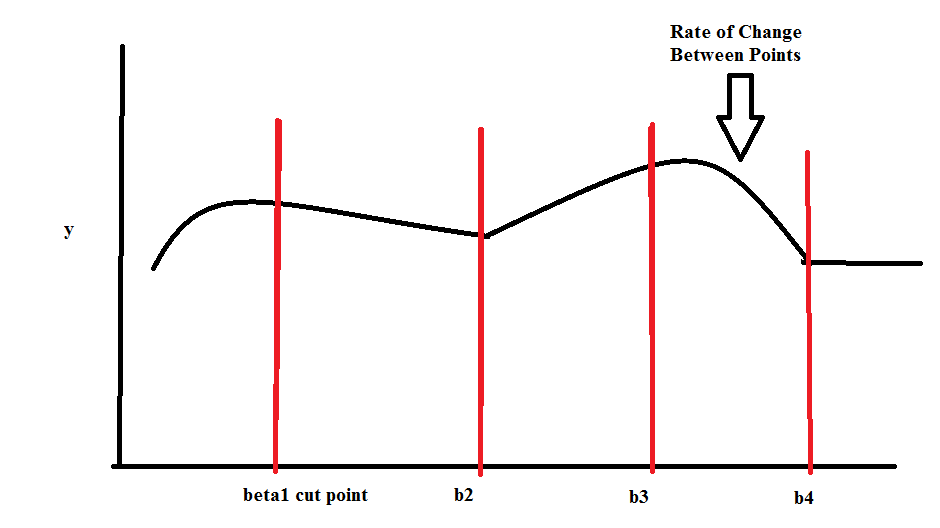
\includegraphics[scale=.65]{yeah}
\end{center}








%------






\clearpage
\subsection{Multinomial Nominal Modeling:}

In multinomial modeling we have categories that have no particular order among them (religious identification for example, or other nominal variables). This is another extension of the binomial regression, except in 0-1 we have 0 all the way up to the $j$th group. The probability of all of these categories have to sum to 1. To use the GLM framework we use the following link function:\\
\begin{equation}
\eta_{ij} = x^{T}_i \beta_j = log \frac{p_{ij}}{p_{i1}} \hspace{.5cm} \forall  \hspace{.5cm}  j = 2, ... , J
\end{equation}
Since these categories have to equal to 1, we can manipulate and set the baseline category (usually whatever is coded 1 in R) to come up with a link that looks very similar to the logistic link, only with a summation operator for the categories starting beyond the omitted category, at $j=2$ to the final category $J$:\\
\begin{equation}
 p_{ij} = \frac{exp(\eta_{ij})}{1+ \Sigma^{J}_{j=2} exp (\eta_{ij})   }
\end{equation}
The only difference between this and the logistic regression is the summation operator for multiple categories rather than just the two in logistic regression. To run multinomial data in \texttt{R} we use the \texttt{nnet} package, which includes a lot on neural networks but also has a great multinomial function:\\


\begin{knitrout}
\definecolor{shadecolor}{rgb}{0.165, 0.169, 0.184}\color{fgcolor}\begin{kframe}
\begin{alltt}
\hlstd{> }\hlkwd{library}\hlstd{(nnet)}
\hlstd{> }\hlstd{object} \hlkwb{<-} \hlkwd{multinom}\hlstd{(formula)}
\end{alltt}
\end{kframe}
\end{knitrout}


The following table is what a multinomial output looks like, created using the \texttt{R faraway} package, utilizing the NES 1996 data. Assume, for some reason, all we needed to add in our model was age and the amount of TV someone watched to predict their partisan leanings. \\



\begin{table}[h!]
\caption{Statistical models}
\begin{center}
\begin{tabular}{l c c }
\hline
 & Independent & Republican \\
\hline
Intercept       & $\mathbf{-2.71}^{*}$ & $-0.36$          \\
                & $[-3.73;\ -1.69]$    & $[-0.76;\ 0.04]$ \\
Age             & $0.01$               & $0.01$           \\
                & $[-0.02;\ 0.03]$     & $[-0.00;\ 0.02]$ \\
TV News         & $-0.06$              & $-0.05$          \\
                & $[-0.19;\ 0.08]$     & $[-0.10;\ 0.01]$ \\
\hline
AIC             & 1571.79              & 1571.79          \\
BIC             & 1600.89              & 1600.89          \\
Log\ Likelihood & -779.90              & -779.90          \\
Deviance        & 1559.79              & 1559.79          \\
Num.\ obs.      & 944                  & 944              \\
\hline
\multicolumn{3}{l}{\scriptsize{$^*$ 0 outside the confidence interval}}
\end{tabular}
\end{center}
\end{table}

The raw coefficient we get is the logged odds from moving from the deleted category (Democrat here) to either Independent or Republican. Logged odds are pretty unituitive however, so making predictive probabilities from multinomial coefficients (and indeed much of regression output) is helpful to readers:

\begin{center}
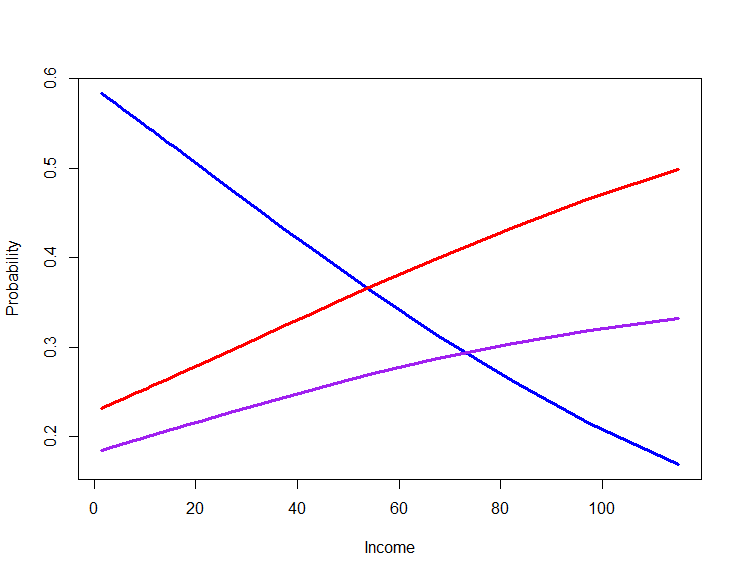
\includegraphics[scale=.7]{IncPlot}
\end{center}

The above plot is modeling income along the x axis and the probability of being Democrat, Republican, or Independent (purple) for the NES 1996 data. This is using the ``predict'' command in R, which generates predictive probabilities out of our coefficients.

\begin{knitrout}
\definecolor{shadecolor}{rgb}{0.165, 0.169, 0.184}\color{fgcolor}\begin{kframe}
\begin{alltt}
\hlstd{> }\hlkwd{predict}\hlstd{(mmodi,}\hlkwd{data.frame}\hlstd{(}\hlkwc{nincome}\hlstd{=il),}\hlkwc{type}\hlstd{=}\hlstr{"probs"}\hlstd{)} \hlcom{# include type="probs"}
\hlstd{> }\hlkwd{predict}\hlstd{(mmodi,}\hlkwd{data.frame}\hlstd{(}\hlkwc{nincome}\hlstd{=il))}
\hlstd{> }
\hlstd{> }\hlcom{# Create Object with this probability matrix}
\hlstd{> }\hlstd{prmat} \hlkwb{<-} \hlkwd{predict}\hlstd{(mmodi,}\hlkwd{data.frame}\hlstd{(}\hlkwc{nincome}\hlstd{=}\hlkwd{sort}\hlstd{(}\hlkwd{unique}\hlstd{(nincome))),}
\hlstd{+ }         \hlkwc{type}\hlstd{=}\hlstr{"probs"}\hlstd{)}
\hlstd{> }
\hlstd{> }\hlcom{# Plotting:}
\hlstd{> }\hlkwd{plot}\hlstd{(}\hlkwd{unique}\hlstd{(nincome), prmat[,}\hlnum{1}\hlstd{],} \hlkwc{type}\hlstd{=}\hlstr{"l"}\hlstd{,} \hlkwc{col}\hlstd{=}\hlstr{"blue"}\hlstd{,} \hlkwc{lwd}\hlstd{=}\hlnum{3}\hlstd{,}
\hlstd{+ }       \hlkwc{xlab}\hlstd{=}\hlstr{"Income"}\hlstd{,} \hlkwc{ylab}\hlstd{=}\hlstr{"Probability"}\hlstd{)} \hlcom{# Labels}
\hlstd{> }\hlkwd{lines}\hlstd{(}\hlkwd{unique}\hlstd{(nincome), prmat[,}\hlnum{3}\hlstd{],} \hlkwc{type}\hlstd{=}\hlstr{"l"}\hlstd{,} \hlkwc{col}\hlstd{=}\hlstr{"red"}\hlstd{,} \hlkwc{lwd}\hlstd{=}\hlnum{3}\hlstd{)}
\hlstd{> }\hlkwd{lines}\hlstd{(}\hlkwd{unique}\hlstd{(nincome), prmat[,}\hlnum{2}\hlstd{],} \hlkwc{type}\hlstd{=}\hlstr{"l"}\hlstd{,} \hlkwc{col}\hlstd{=}\hlstr{"purple"}\hlstd{,} \hlkwc{lwd}\hlstd{=}\hlnum{3}\hlstd{)}
\hlstd{> }
\hlstd{> }\hlkwd{summary}\hlstd{(mmodi)}
\end{alltt}
\end{kframe}
\end{knitrout}








%-----------







\clearpage
\subsection{Survival Modeling:}

Survival models (event history models) take data that occurs over a duration of time and maps the likelihood of surviving until the next ``step''. This could be, for example, the effect of a treatment, the lifeline of a patent in therapy, the tenure of a officeholder, or the length that a bill or law stays active over time. Consider the table:

\begin{knitrout}
\definecolor{shadecolor}{rgb}{0.165, 0.169, 0.184}\color{fgcolor}\begin{kframe}
\begin{alltt}
\hlstd{> }\hlkwd{library}\hlstd{(survminer)}
\hlstd{> }\hlkwd{library}\hlstd{(survival)}
\hlstd{> }
\hlstd{> }\hlcom{# Expoential:}
\hlstd{> }\hlstd{expmod} \hlkwb{<-} \hlkwd{survreg}\hlstd{(}\hlkwd{Surv}\hlstd{(te, censor)} \hlopt{~} \hlstd{wc} \hlopt{+} \hlstd{dem} \hlopt{+} \hlstd{pvote} \hlopt{+} \hlstd{south,}
\hlstd{+ }                  \hlkwc{data} \hlstd{= dat,} \hlkwc{dist} \hlstd{=} \hlstr{"exponential"}\hlstd{)}
\hlstd{> }
\hlstd{> }\hlcom{# Weibull:}
\hlstd{> }\hlstd{weibullmod} \hlkwb{<-} \hlkwd{survreg}\hlstd{(}\hlkwd{Surv}\hlstd{(te, censor)} \hlopt{~} \hlstd{wc} \hlopt{+} \hlstd{dem} \hlopt{+} \hlstd{pvote} \hlopt{+} \hlstd{south,}
\hlstd{+ }                  \hlkwc{data} \hlstd{= dat,} \hlkwc{dist} \hlstd{=} \hlstr{"weibull"}\hlstd{)}
\end{alltt}
\end{kframe}
\end{knitrout}



\begin{table}[h!]
\caption{Survival Models}
\begin{center}
\begin{tabular}{l c c c }
\hline
 & Exponential & Weibull & exp(Cox) \\
\hline
Intercept          & $3.60$    & $3.59$    &           \\
                   & $(0.10)$  & $(0.10)$  &           \\
Investiture        & $-0.36$   & $-0.34$   &           \\
                   & $(0.13)$  & $(0.12)$  &           \\
Polarization       & $-0.039$  & $-0.04$   & $1.04$    \\
                   & $(0.01)$  & $(0.005)$ & $(0.01)$  \\
Crisis Duration    & $0.01$    & $0.01$    & $0.99$    \\
                   & $(0.002)$ & $(0.002)$ & $(0.002)$ \\
Log(Scale)         &           & $-0.12$   &           \\
                   &           & $(0.05)$  &           \\

\hline
Scale              & Fixed 1   & 0.884     &         \\
Log\ Likelihood    & -1056.7   & -1053.8   & 56.6    \\
$\chi^2$           & 88.08     & 93.6      &         \\
df                 &  3        &   3       & 2       \\
Num.\ obs.         & 314       & 314       & 314     \\
\hline
\multicolumn{4}{l}{\scriptsize{Dependent variable: Duration}}
\end{tabular}
\end{center}
\end{table}

The above table is the coefficients and standard errors for two models (and an expoentiated Cox model), the exponential and Weibull of a survival modeling of duration given legislative investiture, polarization measures, and crisis duration (measured in days). Our variable of interest here is the presence of legislative investiture and Gary King's claim that they prevent against failure in international national cabinets (their duration).\footnote{King, Gary, James E. Alt, Nancy Elizabeth Burns and Michael Laver (1990). ``A United Model of Cabinet Dissolution in Parliamentary Democracies," American Journal of Political Science, vol. 34, no. 3, pp. 846-870.}

In interpretation, The exponential model assumes the scale parameter to be uniform for our hazard model (uniform at 1). This, in a basic sign-and-significance interpretation yields negative relationships for investiture policy and polarization which are both significant but weakly influential. The Weibull model gives us the actual scale parameter (.884) and similar results although slightly weaker when accounting for distributional changes additionally the interpretation changes via in absolute value terms from the exponential to the Weibull model. The Cox model assumes that the two strata within the survival curves will be proportional to each other, which could be an easy assumption to fulfill in some theory. Finally, the exponentiation of the Cox model can be read similarly to the Poisson model and is just a measure \textit{of the effect of the hazard rate}, which again is the risk of failure given that the participant has survived up to a specific time. The Cox model output here does not include our strata (investiture).\footnote{\texttt{coxph(Surv(duration, ciep12) $\sim$ strata(invest) + polar + crisis, data = dat,\\
 method = "efron")}}


\begin{center}
\textbf{Figure 1: Exponential Survival Model of Legislative Investiture}
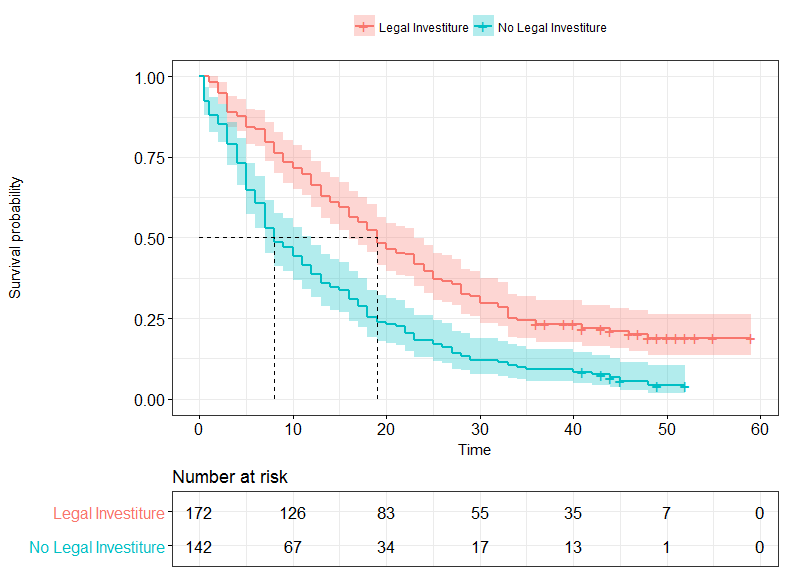
\includegraphics[scale=.65]{Surv}
\end{center}


\clearpage
\begin{center}
\textbf{Figure 2: Cox Survival Model of Legislative Investiture}
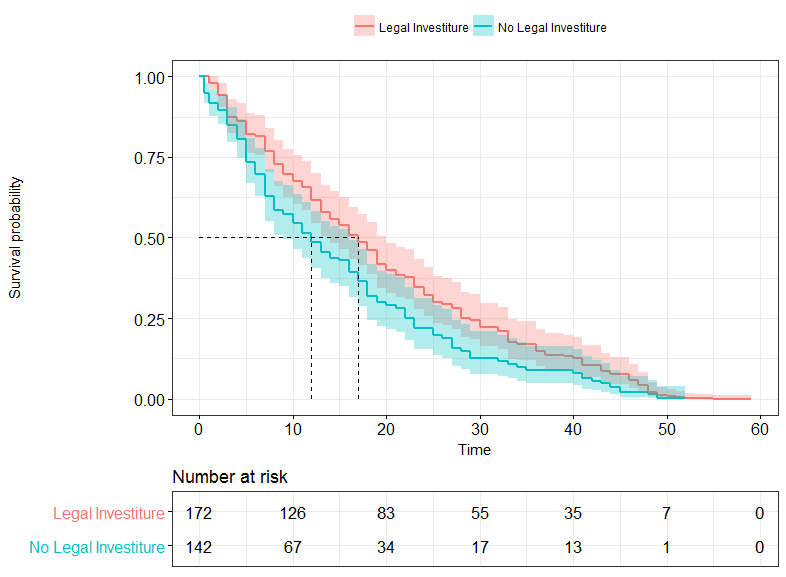
\includegraphics[scale=.65]{Cox}
\end{center}


\begin{knitrout}
\definecolor{shadecolor}{rgb}{0.165, 0.169, 0.184}\color{fgcolor}\begin{kframe}
\begin{alltt}
\hlstd{> }\hlcom{#Survival GGplot Example (not used to replicate above, code as template)}
\hlstd{> }
\hlstd{> }    \hlkwd{ggsurvplot}\hlstd{(fit,} \hlkwc{data} \hlstd{= dataset)}
\hlstd{> }\hlkwd{ggsurvplot}\hlstd{(fit,} \hlkwc{data} \hlstd{= dataset,}
\hlstd{+ }                \hlkwc{surv.median.line} \hlstd{=} \hlstr{"hv"}\hlstd{,}  \hlcom{# Add medians survival}
\hlstd{+ }                        \hlcom{# Change legends: title & labels}
\hlstd{+ }                \hlkwc{legend.title} \hlstd{=} \hlstr{"Title"}\hlstd{,}
\hlstd{+ }                \hlkwc{legend.labs} \hlstd{=} \hlkwd{c}\hlstd{(}\hlstr{"One Category"}\hlstd{,} \hlstr{"Another"}\hlstd{),}
\hlstd{+ }                        \hlcom{# Add p-value and confidence intervals}
\hlstd{+ }                \hlkwc{pval} \hlstd{=} \hlnum{TRUE}\hlstd{,}
\hlstd{+ }                \hlkwc{conf.int} \hlstd{=} \hlnum{TRUE}\hlstd{,}
\hlstd{+ }                        \hlcom{# Add risk table}
\hlstd{+ }                \hlkwc{risk.table} \hlstd{=} \hlnum{TRUE}\hlstd{,}
\hlstd{+ }                \hlkwc{tables.height} \hlstd{=} \hlnum{0.2}\hlstd{,}
\hlstd{+ }                \hlkwc{tables.theme} \hlstd{=} \hlkwd{theme_cleantable}\hlstd{(),}
\hlstd{+ }                \hlcom{#Load "GrandBudapest" color scheme}
\hlstd{+ }                \hlkwc{palette} \hlstd{=} \hlkwd{c}\hlstd{(}\hlkwd{wes_palette}\hlstd{(}\hlstr{"GrandBudapest"}\hlstd{,} \hlnum{2}\hlstd{,}
\hlstd{+ }                \hlkwc{type} \hlstd{=} \hlstr{"discrete"}\hlstd{)[}\hlnum{1}\hlstd{],}
\hlstd{+ }                \hlkwd{wes_palette}\hlstd{(}\hlstr{"GrandBudapest"}\hlstd{,} \hlnum{2}\hlstd{,}
\hlstd{+ }                \hlkwc{type} \hlstd{=} \hlstr{"discrete"}\hlstd{)[}\hlnum{2}\hlstd{]),}
\hlstd{+ }                \hlkwc{ggtheme} \hlstd{=} \hlkwd{theme_bw}\hlstd{()}  \hlcom{#Change ggplot2 theme}
\hlstd{+ }              \hlstd{)}
\end{alltt}
\end{kframe}
\end{knitrout}


\newpage

Survival modeling is a variation of the generalized linear model which accounts for predicted probabilities as a phenomenon or actual actor dies in the course of study. Each depression in the figures is the instance of death in the dependent variable. Exponential modeling holds the hazard as uniform (1) giving us an interpretation of the predicted chance of dying. Weibell, in contrary, is the predicted probability of living and does not make an assumption on the scale parameter and reports this hazard parameter to the researcher (resulting in a loss of one degree of freedom).\footnote{Recall that this is very similar to the scale/variance problem we occurred in Poisson regression. Similarities are very similar here as well, and the math is similar in this respect too.} Confidence intervals for both Figure 1 and 2 are set at 95\% and the number at risk are the remaining participants in the study at each time location. The dotted lines report the median of the data for each strata (Investiture). Finally, given the Kaplan-Meier modeling here each depression is robust in that it controls for a multiple-drop off scenario to where $1/n$ can be calculated. For example, if three people were to die off at the same time point a $1/10, 1/9, 1/8$ would be calculated instead of all three at the same functional moment. The number remaining at risk is shown descriptively below each figure. \\

Interpretation of the actual coefficients is very similar to Poisson modeling given that our general linear model is following similar distribution as the Poisson (non-negative). Yet, the Poisson uses count-integer level data whereas survival modeling can use continuous data. Because of the similarities, the beta coefficient reported is similar, it is the multiplicative effect holding all else constant of a one unit increase in $X$ onto $Y$. \\

I have been able to plot both of these together in base-R; but I don't like how it looks compared to \texttt{ggplot}. \\


\begin{center}
\textbf{Figure 3: Survival Models of Legislative Investiture in Base R}
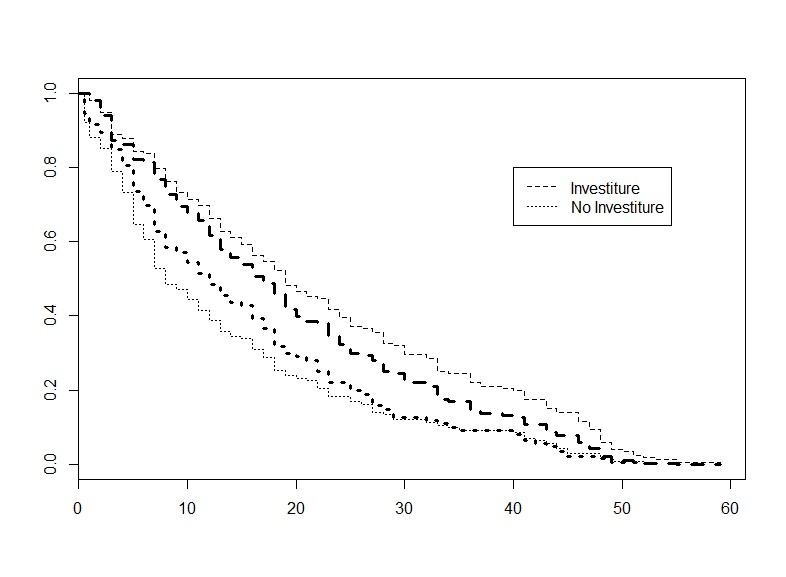
\includegraphics[scale=.6]{SurvR}
\end{center}

\clearpage
\noindent \textbf{Further Notes: Comments}\\
\noindent \textit{Censoring Problem in Survival Models:} \\
Perhaps as an additional note, a unique problem to survival modelings is the issue of censoring. Censoring is where participants (or the observed phenomenon)lives beyond the end point of the study. This is an example of rightward-censoring, but leftward-censoring would just be the inverse (beginning a study beyond the start of the phenomenon). This is a unique and difficult threat to survival models, thus we have had to use much of the tools listed in this section to account for these kinds of data. \footnote{Princeton article here includes mathematically how this and much of survival analysis works:\\
 http://data.princeton.edu/wws509/notes/c7.pdf}

\hfill \\

\noindent \textit{iid:} \\
The GLM nature of the survival model does not give it a free pass on the independent and individually distributed (iid) assumption. In fact, much of the time in dealing with survival-type theories (bill-survival, authoritarian regimes, cancer patients) we deal with responses that are not independent of one-another. A doctor seeing cancer patients, for example, may see twenty patients and as they become fully treated or pass away he may have more time to distribute to other patients. These patients may even meet and have group-therapy among themselves (just as bills may co-vary and authoritarians interlock in strategy)! Further methodology (networks for instance) can help circumvent these concerns.

















\clearpage
\subsection{Conclusion, Quick Reference}

\textbf{The GLM}\\

The general linear model framework consists of a stochastic and systematic component, in order to use other distributions in the exponential family we need a \textit{link function} and to change our distriubtion. These build connections (links) between the mean of the DGP to our linear predictors.\\

\hfill \\
\noindent \textbf{Linear Model}\\
It's origins in geometry, the standard linear model is initially pretty flexible to most social science data. In geometry, $y=mx+b$ can be rewritten for data: $y=\alpha + \beta X$ or $y= \beta_0 + \beta X$. where $\alpha$ or $\beta_0$ is the y-intercept, $\beta_i$ is the $i$th coefficient for each variable onto our dependent variable $y$ and $X$ is our observed independent variable data. \\
In R this is executed simply:\\
\begin{verbatim}
object <- lm(formula)
#formula: (DV ~ IV + IV + IV)
\end{verbatim}

Coefficients received in a standard linear model table are interpreted as a one unit increase in X as an effect on our DV (pg. 4 for more, and probability plotting). \\

\hfill \\
\noindent \textbf{Logit Regression:}

Logit (and the alternative probit) regression(s) examine dependent variables that are coded dichotomous (0;1). This is accomplished by the link function $p\left(\frac{p}{1-p}\right)$.

 If coded correctly, logit regression can give you the logged odds from moving from a zero (event not happening) to one (event happening). Yet, we often don't think in terms of logged odds, so we can calculate predictive probabilities by dividing the coefficient by four - this will yield a maximum predictive probability when the coefficient rests in the middle of the logistic curve. \\

 More helpful for readers, perhaps, is to generate a probability plot, including data points along the x axis and the probability(y) along the logistic curve on the y axis. \\

\clearpage
\noindent \textbf{Poisson Regression:}\\
Poisson, Quasi-Poisson, and Negative Binomial regression all take count level data. Poisson assumes the variance to be held equal to the mean (a ``1'' in Quasi-Poisson); whereas Quasi-Poisson and Negative Binomial allow the variance to differentiate between models. In R:\\

\begin{knitrout}
\definecolor{shadecolor}{rgb}{0.165, 0.169, 0.184}\color{fgcolor}\begin{kframe}
\begin{alltt}
\hlstd{> }\hlcom{# Poisson}
\hlstd{> }\hlstd{object} \hlkwb{<-} \hlkwd{glm}\hlstd{(formula,} \hlkwc{family} \hlstd{= poisson)}
\hlstd{> }
\hlstd{> }\hlcom{# Quasi-Poisson}
\hlstd{> }\hlstd{object} \hlkwb{<-} \hlkwd{glm}\hlstd{(formula,} \hlkwc{family} \hlstd{= quasipoisson)}
\hlstd{> }
\hlstd{> }\hlcom{# Negative Binomial/ Gamma-Poisson}
\hlstd{> }\hlstd{object} \hlkwb{<-} \hlkwd{glm.nb}\hlstd{(formula)}
\end{alltt}
\end{kframe}
\end{knitrout}

For interpretation, it is best to exponentiate the coefficients ($e^\beta$) to receive the multiplicative change exerted from each variable (keeping in mind significance). Tables can be created that show readers these effects (pg. 18-19).


\hfill \\
\noindent \textbf{Ordinal Regression:}\\
Ordinal data requires the interpretation of cut points ($k$) within our regression and is interpreted similarly to logistic regression. Ordinal data between cut points can be thought of as a series of logistic regressions between cut points.


\begin{knitrout}
\definecolor{shadecolor}{rgb}{0.165, 0.169, 0.184}\color{fgcolor}\begin{kframe}
\begin{alltt}
\hlstd{> }\hlcom{# Ordinal Regression}
\hlstd{> }\hlstd{object} \hlkwb{<-} \hlkwd{polr}\hlstd{(formula)}
\end{alltt}
\end{kframe}
\end{knitrout}


It is important to make note of the ordinal categories, one category is omitted as a reference category within regression and the information received is in refference to the omitted category. Inverse logit subtraction can yield predictive probabilities: $logit^{-1}(\theta_{k+1}) - logit^{-1}(\theta_k) $ these latent space estimates are important to note as, when controlling for all else, the relative change between ordinal responses (feeling ``okay'' to feeling ``great'' for example).

\hfill \\




\noindent \textbf{Multinomial Nominal Modeling:}

\begin{knitrout}
\definecolor{shadecolor}{rgb}{0.165, 0.169, 0.184}\color{fgcolor}\begin{kframe}
\begin{alltt}
\hlstd{> }\hlkwd{library}\hlstd{(nnet)}
\hlstd{> }\hlstd{object} \hlkwb{<-} \hlkwd{multinom}\hlstd{(formula)}
\end{alltt}
\end{kframe}
\end{knitrout}


Multinomial modeling includes data that is non-ordered, for example religious identity. Mathematically the link function (considering all probabilities for each category need add up to one) is very similar to the logistic link.

With the raw coefficients we get from multinomial data we receive the logged odds (like logistic regression) from moving from the omitted category (usually the first category in R) to the following categories. Again, we don't typically think in logged odds (another similarity to logistic regression) so making predictive probability plots are helpful (again, similar to logistic regression). \\


\hfill \\
\noindent \textbf{Survival Modeling: }

Survival models (as the name suggests) measures and indeed explicitly addresses the length of time a unit dies or survives across a length of time. The hazard parameter is held constant in the exponential model (at 1) whereas in the Weibull model it is allowed to vary (losing one degree of freedom, but this choice would depend on theory). To model survival data:

\begin{knitrout}
\definecolor{shadecolor}{rgb}{0.165, 0.169, 0.184}\color{fgcolor}\begin{kframe}
\begin{alltt}
\hlstd{> }\hlkwd{library}\hlstd{(survminer)}
\hlstd{> }\hlkwd{library}\hlstd{(survival)}
\hlstd{> }
\hlstd{> }\hlstd{expmod} \hlkwb{<-} \hlkwd{survreg}\hlstd{(}\hlkwd{Surv}\hlstd{(te, censor)} \hlopt{~} \hlstd{wc} \hlopt{+} \hlstd{dem} \hlopt{+} \hlstd{pvote} \hlopt{+} \hlstd{south,}
\hlstd{+ }                  \hlkwc{data} \hlstd{= dat,} \hlkwc{dist} \hlstd{=} \hlstr{"exponential"}\hlstd{)}
\hlstd{> }
\hlstd{> }\hlstd{weibullmod} \hlkwb{<-} \hlkwd{survreg}\hlstd{(}\hlkwd{Surv}\hlstd{(te, censor)} \hlopt{~} \hlstd{wc} \hlopt{+} \hlstd{dem} \hlopt{+} \hlstd{pvote} \hlopt{+} \hlstd{south,}
\hlstd{+ }                  \hlkwc{data} \hlstd{= dat,} \hlkwc{dist} \hlstd{=} \hlstr{"weibull"}\hlstd{)}
\end{alltt}
\end{kframe}
\end{knitrout}



In interpretation of these models' output, we should consider it similar to the Poisson modeling: the multiplicative effect, holding all else constant, of a one unit increase in X onto Y. Although predictive probability plots are (again) superior to present these results.

Mapping graphs as shown in full in Section 7, are a intuitive and attractive way to communicate results to the reader. In these we separate two interesting strata and map the survival data accordingly, controlling for what we deem important with our theory. Kaplan-Meier \index{Kaplan-Meier} checks are also important because multiple ``deaths'' could occur at once and this will scale each of these instead of all at once - which is better.









\clearpage
\section{Machine Learning}

Machine learning has come to be popular among data scientists, chiefly for its ability to remove the researcher and have more streamlined ways to emperically examine categorization and estimands. By definition there are two types of machine learning, supervised and unsupervised. The prior includes researcher influence, classifications and penalizing regressions. The latter includes algarithmic detections of classifications and estimands through a (dare I say) machine-like process.

\

\textit{Types of Machine Learning}
\begin{equation}\nonumber
\begin{cases}
\text{Supervised learning} \begin{cases} \text{Classification} \\ \text{Regression} \end{cases}\\
\text{Unsupervised learning} \begin{cases} \text{Discovering clusters} \\ \text{Discovering latent factors} \\ \text{Discovering graph structure} \\ \text{Matrix completion} \end{cases}\\
\end{cases}
\end{equation}

A large benefit of this section will come in making synthetic data to test some fundemental assumptions of the GLM, all before introducing machine learning as a way to help us reach similar or better conclusions without the threat of researcher bias and ensured reproducability. For this reason, even an novice to graduate methods may find helpful the code and testing that exists in this section, as I have.

\subsection{Simulation and Replication}

Let's begin by setting up a simulated regression, which will have similar architecture throughout this chapter. This particular regression will have two random variables ($x_1$ and $x_2$) for $N$ observations. Then, we create our own coefficent values ($\beta$) and errors ($e$). A vector of ones is our intercept ($alpha$) and this is all neatly placed into a matrix. From this random data we can test some intial regressions.

\begin{knitrout}
\definecolor{shadecolor}{rgb}{0.165, 0.169, 0.184}\color{fgcolor}\begin{kframe}
\begin{alltt}
\hlstd{> }\hlkwd{set.seed}\hlstd{(}\hlnum{12345}\hlstd{)}
\hlstd{> }
\hlstd{> }\hlstd{N} \hlkwb{<-} \hlnum{1000}
\hlstd{> }\hlcom{# Two random x variables, with same mean and same error. Distributed Normally}
\hlstd{> }\hlstd{x_1} \hlkwb{<-} \hlkwd{rnorm}\hlstd{(N,} \hlkwc{mean}\hlstd{=}\hlnum{5}\hlstd{,} \hlkwc{sd}\hlstd{=}\hlkwd{sqrt}\hlstd{(}\hlnum{16}\hlstd{))}
\hlstd{> }\hlstd{x_2} \hlkwb{<-} \hlkwd{rnorm}\hlstd{(N,} \hlkwc{mean}\hlstd{=}\hlnum{5}\hlstd{,} \hlkwc{sd}\hlstd{=}\hlkwd{sqrt}\hlstd{(}\hlnum{16}\hlstd{))}
\hlstd{> }\hlcom{# beta values to multiply with the Intercept, X_1, and X_2 matrix.}
\hlstd{> }\hlstd{b} \hlkwb{<-} \hlkwd{c}\hlstd{(}\hlnum{2}\hlstd{,} \hlopt{-}\hlnum{1}\hlstd{,} \hlnum{3}\hlstd{)}
\hlstd{> }\hlcom{# Perfect-world errors: e~Normal(0, sig^2). set pretty low, Number=1000}
\hlstd{> }\hlstd{e} \hlkwb{<-} \hlkwd{rnorm}\hlstd{(N,} \hlnum{0}\hlstd{,} \hlkwc{sd}\hlstd{=}\hlkwd{sqrt}\hlstd{(}\hlnum{4}\hlstd{))}
\hlstd{> }\hlcom{# This vector of ones is to generate our intercept along with the "2" in our beta}
\hlstd{> }\hlstd{ones} \hlkwb{<-} \hlkwd{matrix}\hlstd{(}\hlnum{1}\hlstd{,} \hlkwc{nrow}\hlstd{=}\hlnum{1000}\hlstd{,} \hlkwc{ncol}\hlstd{=}\hlnum{1}\hlstd{)}
\hlstd{> }\hlstd{X} \hlkwb{<-} \hlkwd{matrix}\hlstd{(}\hlkwd{c}\hlstd{(ones, x_1, x_2),} \hlkwc{nrow}\hlstd{=N)}
\hlstd{> }\hlcom{# head(X)  # Checked that the Matrix comes out right, and is intuitive}
\hlstd{> }\hlcom{# y = intercept + b1*X_1 + b2*X_2 + some error}
\hlstd{> }\hlstd{y} \hlkwb{<-} \hlstd{b[}\hlnum{1}\hlstd{]}\hlopt{*}\hlstd{X[,}\hlnum{1}\hlstd{]}\hlopt{+} \hlstd{b[}\hlnum{2}\hlstd{]}\hlopt{*}\hlstd{X[,}\hlnum{2}\hlstd{]}\hlopt{+} \hlstd{b[}\hlnum{3}\hlstd{]}\hlopt{*}\hlstd{X[,}\hlnum{3}\hlstd{]} \hlopt{+} \hlstd{e}
\hlstd{> }\hlstd{my_data} \hlkwb{<-} \hlkwd{data.frame}\hlstd{(x_1, x_2, y)}
\hlstd{> }\hlcom{# After having y, we can run our formula, OLS using lm()}
\hlstd{> }\hlstd{m1} \hlkwb{<-} \hlkwd{lm}\hlstd{(y} \hlopt{~} \hlstd{x_1} \hlopt{+} \hlstd{x_2,} \hlkwc{data}\hlstd{=my_data)}
\hlstd{> }\hlkwd{summary}\hlstd{(m1)}\hlopt{$}\hlstd{coef}
\end{alltt}
\begin{verbatim}
##              Estimate Std. Error   t value     Pr(>|t|)
## (Intercept)  1.992134 0.12163219  16.37834 1.420043e-53
## x_1         -1.005716 0.01517949 -66.25491 0.000000e+00
## x_2          2.997224 0.01503489 199.35128 0.000000e+00
\end{verbatim}
\end{kframe}
\end{knitrout}

We find that our estimates in our model come very close to our defined beta estimates, this makes sense since our betas were pre-defined this way. Each variable is statistically significant given we entered a pretty low error value into the model. Let's take the above regression and simulate it 1,000 times through a loop:

\begin{knitrout}
\definecolor{shadecolor}{rgb}{0.165, 0.169, 0.184}\color{fgcolor}\begin{kframe}
\begin{alltt}
\hlstd{> }\hlcom{# Let's set up an Empty matrix}
\hlstd{> }\hlstd{simulation1} \hlkwb{<-} \hlkwd{matrix}\hlstd{(}\hlkwc{nrow} \hlstd{=} \hlnum{1000}\hlstd{,} \hlkwc{ncol} \hlstd{=} \hlnum{6}\hlstd{)}
\hlstd{> }\hlcom{# head(simulation1)  # Matrix of NA's to fill in simulated values later.}
\hlstd{> }
\hlstd{> }\hlkwa{for} \hlstd{(i} \hlkwa{in} \hlnum{1}\hlopt{:}\hlnum{1000}\hlstd{)}
\hlstd{+ }\hlstd{\{}
\hlstd{+ }  \hlstd{N} \hlkwb{<-} \hlnum{1000}
\hlstd{+ }  \hlstd{x_1} \hlkwb{<-} \hlkwd{rnorm}\hlstd{(N,} \hlkwc{mean}\hlstd{=}\hlnum{5}\hlstd{,} \hlkwc{sd}\hlstd{=}\hlkwd{sqrt}\hlstd{(}\hlnum{16}\hlstd{))}
\hlstd{+ }  \hlstd{x_2} \hlkwb{<-} \hlkwd{rnorm}\hlstd{(N,} \hlkwc{mean}\hlstd{=}\hlnum{5}\hlstd{,} \hlkwc{sd}\hlstd{=}\hlkwd{sqrt}\hlstd{(}\hlnum{16}\hlstd{))}
\hlstd{+ }  \hlstd{b} \hlkwb{<-} \hlkwd{c}\hlstd{(}\hlnum{2}\hlstd{,} \hlopt{-}\hlnum{1}\hlstd{,} \hlnum{3}\hlstd{)}
\hlstd{+ }  \hlstd{e} \hlkwb{<-} \hlkwd{rnorm}\hlstd{(N,} \hlnum{0}\hlstd{,} \hlkwc{sd}\hlstd{=}\hlkwd{sqrt}\hlstd{(}\hlnum{4}\hlstd{))}
\hlstd{+ }  \hlstd{ones} \hlkwb{<-} \hlkwd{matrix}\hlstd{(}\hlnum{1}\hlstd{,} \hlkwc{nrow}\hlstd{=}\hlnum{1000}\hlstd{,} \hlkwc{ncol}\hlstd{=}\hlnum{1}\hlstd{)}
\hlstd{+ }  \hlstd{X} \hlkwb{<-} \hlkwd{matrix}\hlstd{(}\hlkwd{c}\hlstd{(ones, x_1, x_2),} \hlkwc{nrow}\hlstd{=N)}
\hlstd{+ }  \hlstd{y} \hlkwb{<-} \hlstd{b[}\hlnum{1}\hlstd{]}\hlopt{*}\hlstd{X[,}\hlnum{1}\hlstd{]}\hlopt{+} \hlstd{b[}\hlnum{2}\hlstd{]}\hlopt{*}\hlstd{X[,}\hlnum{2}\hlstd{]}\hlopt{+} \hlstd{b[}\hlnum{3}\hlstd{]}\hlopt{*}\hlstd{X[,}\hlnum{3}\hlstd{]} \hlopt{+} \hlstd{e}
\hlstd{+ }  \hlstd{my_data} \hlkwb{<-} \hlkwd{data.frame}\hlstd{(x_1, x_2, y)}
\hlstd{+ }  \hlstd{m1} \hlkwb{<-} \hlkwd{lm}\hlstd{(y} \hlopt{~} \hlstd{x_1} \hlopt{+} \hlstd{x_2)}

\hlstd{+ }  \hlstd{sm1} \hlkwb{<-} \hlkwd{summary}\hlstd{(m1)}  \hlcom{# summary table is used to easily locate standard errors (se)}

\hlstd{+ }  \hlstd{simulation1[i,}\hlnum{1}\hlstd{]} \hlkwb{<-} \hlstd{m1}\hlopt{$}\hlstd{coef[}\hlnum{1}\hlstd{]}    \hlcom{# storing models first coef: Intercept}
\hlstd{+ }  \hlstd{simulation1[i,}\hlnum{2}\hlstd{]} \hlkwb{<-} \hlstd{m1}\hlopt{$}\hlstd{coef[}\hlnum{2}\hlstd{]}    \hlcom{# x_1 coef estimate}
\hlstd{+ }  \hlstd{simulation1[i,}\hlnum{3}\hlstd{]} \hlkwb{<-} \hlstd{m1}\hlopt{$}\hlstd{coef[}\hlnum{3}\hlstd{]}    \hlcom{# x_2 coef estimate}
\hlstd{+ }  \hlstd{simulation1[i,}\hlnum{4}\hlstd{]} \hlkwb{<-} \hlstd{sm1}\hlopt{$}\hlstd{coefficients[}\hlnum{1}\hlstd{,}\hlnum{2}\hlstd{]}   \hlcom{# standard error for Intercept}
\hlstd{+ }  \hlstd{simulation1[i,}\hlnum{5}\hlstd{]} \hlkwb{<-} \hlstd{sm1}\hlopt{$}\hlstd{coefficients[}\hlnum{2}\hlstd{,}\hlnum{2}\hlstd{]}   \hlcom{# se x_1}
\hlstd{+ }  \hlstd{simulation1[i,}\hlnum{6}\hlstd{]} \hlkwb{<-} \hlstd{sm1}\hlopt{$}\hlstd{coefficients[}\hlnum{3}\hlstd{,}\hlnum{2}\hlstd{]}   \hlcom{# se x_2}
\hlstd{+ }\hlstd{\}}
\hlstd{> }
\hlstd{> }\hlcom{# head(simulation1)  # To check our now-full matrix to see if values make sense}
\end{alltt}
\end{kframe}
\end{knitrout}

Next, we will do the same simulation but removing x_2 in our model. Then we will plot each of the variables from the two simulations.The code for plotting has been witheld to save space on page, but it is done using ggplot and a function to make the plots appear next to one another.

\begin{knitrout}
\definecolor{shadecolor}{rgb}{0.165, 0.169, 0.184}\color{fgcolor}\begin{kframe}
\begin{alltt}
\hlstd{> }\hlcom{# Removing x_2 now}
\hlstd{> }\hlcom{#  New empty matrix}
\hlstd{> }\hlstd{simulation2} \hlkwb{<-} \hlkwd{matrix}\hlstd{(}\hlkwc{nrow} \hlstd{=} \hlnum{1000}\hlstd{,} \hlkwc{ncol} \hlstd{=} \hlnum{4}\hlstd{)}
\hlstd{> }\hlcom{# head(simulation2)}
\hlstd{> }
\hlstd{> }\hlkwa{for} \hlstd{(i} \hlkwa{in} \hlnum{1}\hlopt{:}\hlnum{1000}\hlstd{)}
\hlstd{+ }\hlstd{\{}
\hlstd{+ }  \hlstd{N} \hlkwb{<-} \hlnum{1000}
\hlstd{+ }  \hlstd{x_1} \hlkwb{<-} \hlkwd{rnorm}\hlstd{(N,} \hlkwc{mean}\hlstd{=}\hlnum{5}\hlstd{,} \hlkwc{sd}\hlstd{=}\hlkwd{sqrt}\hlstd{(}\hlnum{16}\hlstd{))}
\hlstd{+ }  \hlstd{x_2} \hlkwb{<-} \hlkwd{rnorm}\hlstd{(N,} \hlkwc{mean}\hlstd{=}\hlnum{5}\hlstd{,} \hlkwc{sd}\hlstd{=}\hlkwd{sqrt}\hlstd{(}\hlnum{16}\hlstd{))}
\hlstd{+ }  \hlstd{b} \hlkwb{<-} \hlkwd{c}\hlstd{(}\hlnum{2}\hlstd{,} \hlopt{-}\hlnum{1}\hlstd{,} \hlnum{3}\hlstd{)}
\hlstd{+ }  \hlstd{e} \hlkwb{<-} \hlkwd{rnorm}\hlstd{(N,} \hlnum{0}\hlstd{,} \hlkwc{sd}\hlstd{=}\hlkwd{sqrt}\hlstd{(}\hlnum{4}\hlstd{))}
\hlstd{+ }  \hlstd{ones} \hlkwb{<-} \hlkwd{matrix}\hlstd{(}\hlnum{1}\hlstd{,} \hlkwc{nrow}\hlstd{=}\hlnum{1000}\hlstd{,} \hlkwc{ncol}\hlstd{=}\hlnum{1}\hlstd{)}
\hlstd{+ }  \hlstd{X} \hlkwb{<-} \hlkwd{matrix}\hlstd{(}\hlkwd{c}\hlstd{(ones, x_1, x_2),} \hlkwc{nrow}\hlstd{=N)}
\hlstd{+ }  \hlstd{y} \hlkwb{<-} \hlstd{b[}\hlnum{1}\hlstd{]}\hlopt{*}\hlstd{X[,}\hlnum{1}\hlstd{]}\hlopt{+} \hlstd{b[}\hlnum{2}\hlstd{]}\hlopt{*}\hlstd{X[,}\hlnum{2}\hlstd{]}\hlopt{+} \hlstd{b[}\hlnum{3}\hlstd{]}\hlopt{*}\hlstd{X[,}\hlnum{3}\hlstd{]} \hlopt{+} \hlstd{e}
\hlstd{+ }  \hlstd{m1} \hlkwb{<-} \hlkwd{lm}\hlstd{(y} \hlopt{~} \hlstd{x_1)}                \hlcom{#! no X_2 regressed, but included in DGP}

\hlstd{+ }  \hlstd{sm1} \hlkwb{<-} \hlkwd{summary}\hlstd{(m1)}

\hlstd{+ }  \hlstd{simulation2[i,}\hlnum{1}\hlstd{]} \hlkwb{<-} \hlstd{sm1}\hlopt{$}\hlstd{coef[}\hlnum{1}\hlstd{,}\hlnum{1}\hlstd{]}     \hlcom{#Storing models first coef, Intercept}
\hlstd{+ }  \hlstd{simulation2[i,}\hlnum{2}\hlstd{]} \hlkwb{<-} \hlstd{sm1}\hlopt{$}\hlstd{coef[}\hlnum{2}\hlstd{,}\hlnum{1}\hlstd{]}     \hlcom{#x_1 coef estimate}
\hlstd{+ }  \hlstd{simulation2[i,}\hlnum{3}\hlstd{]} \hlkwb{<-} \hlstd{sm1}\hlopt{$}\hlstd{coef[}\hlnum{1}\hlstd{,}\hlnum{2}\hlstd{]}      \hlcom{#standard error for Intercept}
\hlstd{+ }  \hlstd{simulation2[i,}\hlnum{4}\hlstd{]} \hlkwb{<-} \hlstd{sm1}\hlopt{$}\hlstd{coef[}\hlnum{2}\hlstd{,}\hlnum{2}\hlstd{]}      \hlcom{#se for x_1}
\hlstd{+ }\hlstd{\}}
\hlstd{> }
\hlstd{> }\hlcom{# Full Model Means}
\hlstd{> }\hlcom{#   mean(simulation1[,1]) # mean estimate for b_0 (= 2)}
\hlstd{> }\hlcom{#   mean(simulation1[,2]) # mean estimate for b_1 X_1 estimate (= -1)}
\hlstd{> }\hlcom{#   mean(simulation1[,3]) # mean estimate for b_2 x_2 estimate (= 3)}
\hlstd{> }
\hlstd{> }\hlcom{# Limited Model Means}
\hlstd{> }\hlcom{#   mean(simulation2[,1]) #mean b_0 (=2)}
\hlstd{> }\hlcom{#   mean(simulation2[,2]) #mean b_1 of x_1 (=-1)}
\hlstd{> }\hlcom{# This makes sense given our initial model data b=c(2, -1, 3)}
\end{alltt}
\end{kframe}
\end{knitrout}

\begin{center}
\begin{knitrout}
\definecolor{shadecolor}{rgb}{0.165, 0.169, 0.184}\color{fgcolor}
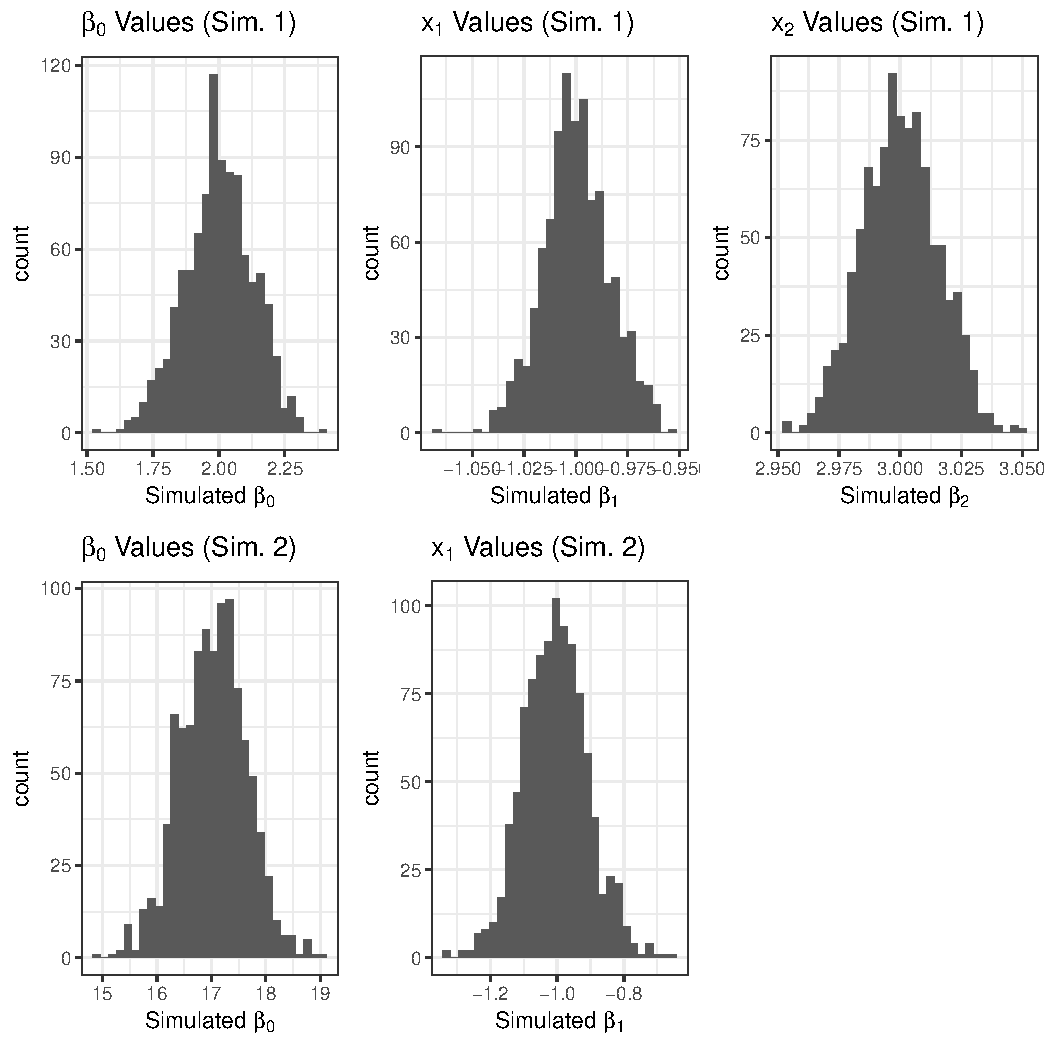
\includegraphics[width=\maxwidth]{figure/PlottingSimulationML-1} 

\end{knitrout}
\end{center}

As is expected, most things remain the same between the two simulations, however in simulation two removing a variable (imagine this being race, education, or some economic variable) biases our estimate of the intercept. More importantly, this will balloon the errors (hopefully because that's what errors are supposed to tell us): \index{Simulation}

\begin{knitrout}
\definecolor{shadecolor}{rgb}{0.165, 0.169, 0.184}\color{fgcolor}\begin{kframe}
\begin{alltt}
\hlstd{> }\hlkwd{mean}\hlstd{(simulation1[,}\hlnum{5}\hlstd{])} \hlcom{# Simulation 1's X_1 se's (0.0158)}
\end{alltt}
\begin{verbatim}
## [1] 0.01581834
\end{verbatim}
\begin{alltt}
\hlstd{> }\hlkwd{mean}\hlstd{(simulation2[,}\hlnum{4}\hlstd{])} \hlcom{# Simulation 2's X_1 se's (0.0962)}
\end{alltt}
\begin{verbatim}
## [1] 0.09632281
\end{verbatim}
\begin{alltt}
\hlstd{> }\hlkwd{mean}\hlstd{(simulation1[,}\hlnum{4}\hlstd{])}  \hlcom{# Simulation 1's Intercept se (.128)}
\end{alltt}
\begin{verbatim}
## [1] 0.1285995
\end{verbatim}
\begin{alltt}
\hlstd{> }\hlkwd{mean}\hlstd{(simulation2[,}\hlnum{3}\hlstd{])}  \hlcom{# Simulation 2's Intercept se (.615)}
\end{alltt}
\begin{verbatim}
## [1] 0.6168927
\end{verbatim}
\begin{alltt}
\hlstd{> }\hlcom{# Errors are larger when we take x_2 out of our analysis}
\hlstd{> }\hlcom{#   (less variation captured from DGP)}
\end{alltt}
\end{kframe}
\end{knitrout}

One advantage of using simulated data is the complete controll and education available from messing around with things without any consequences (most of the time). Now that we have tested some of the fundementals of the linear model and reporting estimates, let's use simulation to try to fit a linear model to binary data.

Let us start with just making a fun function that creates inverse logit estimands.

\begin{knitrout}
\definecolor{shadecolor}{rgb}{0.165, 0.169, 0.184}\color{fgcolor}\begin{kframe}
\begin{alltt}
\hlstd{> }\hlstd{inv.logit} \hlkwb{=} \hlkwa{function}\hlstd{(}\hlkwc{x}\hlstd{)\{}
\hlstd{+ }  \hlkwa{if}\hlstd{(}\hlopt{!}\hlkwd{is.numeric}\hlstd{(x))\{}\hlkwd{return}\hlstd{(}\hlstr{"Error 404: Numbers Not Found"}\hlstd{)\}}
\hlstd{+ }  \hlkwd{exp}\hlstd{(x)}\hlopt{/}\hlstd{(}\hlnum{1}\hlopt{+}\hlkwd{exp}\hlstd{(x))}
\hlstd{+ }\hlstd{\}}
\hlstd{> }
\hlstd{> }\hlkwd{inv.logit}\hlstd{(}\hlnum{.95}\hlstd{)}
\end{alltt}
\begin{verbatim}
## [1] 0.7211152
\end{verbatim}
\begin{alltt}
\hlstd{> }\hlkwd{inv.logit}\hlstd{(}\hlstr{"Normative"}\hlstd{)}
\end{alltt}
\begin{verbatim}
## [1] "Error 404: Numbers Not Found"
\end{verbatim}
\end{kframe}
\end{knitrout}

Now, like before, we will construct a DGP via simulation:

\begin{knitrout}
\definecolor{shadecolor}{rgb}{0.165, 0.169, 0.184}\color{fgcolor}\begin{kframe}
\begin{alltt}
\hlstd{> }\hlkwd{library}\hlstd{(Rlab)} \hlcom{# for rbern() function}
\hlstd{> }\hlstd{simulation5} \hlkwb{<-} \hlkwd{matrix}\hlstd{(}\hlkwc{nrow} \hlstd{=} \hlnum{1000}\hlstd{,} \hlkwc{ncol} \hlstd{=} \hlnum{6}\hlstd{)}
\hlstd{> }\hlcom{# head(simulation5)}
\hlstd{> }
\hlstd{> }\hlkwa{for} \hlstd{(i} \hlkwa{in} \hlnum{1}\hlopt{:}\hlnum{1000}\hlstd{)}
\hlstd{+ }\hlstd{\{}
\hlstd{+ }  \hlstd{N} \hlkwb{<-} \hlnum{1000}
\hlstd{+ }  \hlstd{mu} \hlkwb{<-} \hlkwd{c}\hlstd{(}\hlnum{5}\hlstd{,}\hlnum{5}\hlstd{)}
\hlstd{+ }  \hlstd{Sigma} \hlkwb{<-} \hlkwd{matrix}\hlstd{(} \hlkwd{c}\hlstd{(}\hlnum{2}\hlstd{,} \hlnum{.5}\hlstd{,} \hlnum{.5}\hlstd{,} \hlnum{3} \hlstd{),} \hlkwc{nrow} \hlstd{=} \hlnum{2}\hlstd{,} \hlkwc{ncol}\hlstd{=} \hlnum{2}\hlstd{)}
\hlstd{+ }  \hlstd{mvr} \hlkwb{<-} \hlkwd{mvrnorm}\hlstd{(N, mu, Sigma)} \hlcom{# using MASS package}
\hlstd{+ }  \hlstd{b} \hlkwb{<-} \hlkwd{c}\hlstd{(}\hlnum{.2}\hlstd{,} \hlopt{-}\hlnum{1}\hlstd{,} \hlnum{1.2}\hlstd{)}
\hlstd{+ }  \hlstd{e} \hlkwb{<-} \hlkwd{rnorm}\hlstd{(N,} \hlnum{0}\hlstd{,} \hlkwc{sd}\hlstd{=}\hlkwd{sqrt}\hlstd{(}\hlnum{4}\hlstd{))}
\hlstd{+ }  \hlstd{ones} \hlkwb{<-} \hlkwd{matrix}\hlstd{(}\hlnum{1}\hlstd{,} \hlkwc{nrow}\hlstd{=}\hlnum{1000}\hlstd{,} \hlkwc{ncol}\hlstd{=}\hlnum{1}\hlstd{)}
\hlstd{+ }  \hlstd{X} \hlkwb{<-} \hlkwd{matrix}\hlstd{(}\hlkwd{c}\hlstd{(ones, mvr[,}\hlnum{1}\hlstd{], mvr[,}\hlnum{2}\hlstd{]),} \hlkwc{nrow}\hlstd{=N)}
\hlstd{+ }  \hlstd{y} \hlkwb{<-} \hlstd{b[}\hlnum{1}\hlstd{]}\hlopt{*}\hlstd{X[,}\hlnum{1}\hlstd{]}\hlopt{+} \hlstd{b[}\hlnum{2}\hlstd{]}\hlopt{*}\hlstd{X[,}\hlnum{2}\hlstd{]}\hlopt{+} \hlstd{b[}\hlnum{3}\hlstd{]}\hlopt{*}\hlstd{X[,}\hlnum{3}\hlstd{]} \hlopt{+} \hlstd{e}
\hlstd{+ }  \hlstd{y} \hlkwb{<-} \hlkwd{as.numeric}\hlstd{(y} \hlopt{>=} \hlkwd{median}\hlstd{(y))} \hlcom{# Setting y 0-1 based around median.}

\hlstd{+ }  \hlcom{# Inverse Logits}
\hlstd{+ }  \hlcom{# Intercept}
\hlstd{+ }  \hlstd{inv.logit.a} \hlkwb{<-} \hlkwd{inv.logit}\hlstd{(b[}\hlnum{1}\hlstd{]}\hlopt{*}\hlstd{X[,}\hlnum{1}\hlstd{])}
\hlstd{+ }  \hlstd{b0} \hlkwb{<-} \hlkwd{matrix}\hlstd{(inv.logit.a,} \hlkwc{nrow}\hlstd{=N,} \hlkwc{ncol}\hlstd{=} \hlnum{1}\hlstd{)}

\hlstd{+ }  \hlcom{#X_1}
\hlstd{+ }  \hlstd{inv.logit.x2} \hlkwb{<-} \hlkwd{inv.logit}\hlstd{(b[}\hlnum{2}\hlstd{]}\hlopt{*}\hlstd{X[,}\hlnum{2}\hlstd{])}
\hlstd{+ }  \hlstd{b1} \hlkwb{<-} \hlkwd{matrix}\hlstd{(inv.logit.x2,} \hlkwc{nrow}\hlstd{=N,} \hlkwc{ncol}\hlstd{=} \hlnum{1}\hlstd{)}

\hlstd{+ }  \hlcom{#X_2}
\hlstd{+ }  \hlstd{inv.logit.x3} \hlkwb{<-} \hlkwd{inv.logit}\hlstd{(b[}\hlnum{3}\hlstd{]}\hlopt{*}\hlstd{X[,}\hlnum{3}\hlstd{])}
\hlstd{+ }  \hlstd{b2} \hlkwb{<-} \hlkwd{matrix}\hlstd{(inv.logit.x3,} \hlkwc{nrow}\hlstd{=N,} \hlkwc{ncol}\hlstd{=} \hlnum{1}\hlstd{)}

\hlstd{+ }  \hlstd{pi} \hlkwb{<-} \hlkwd{matrix}\hlstd{(}\hlkwd{c}\hlstd{(b0, b1, b2),} \hlkwc{nrow}\hlstd{=N,} \hlkwc{ncol}\hlstd{=}\hlnum{3}\hlstd{)}
\hlstd{+ }  \hlstd{y} \hlkwb{<-} \hlkwd{rbern}\hlstd{(N, pi)}

\hlstd{+ }  \hlstd{m5} \hlkwb{<-} \hlkwd{lm}\hlstd{(y} \hlopt{~} \hlstd{X[,}\hlnum{2}\hlstd{]}\hlopt{+} \hlstd{X[,}\hlnum{3}\hlstd{])} \hlcom{# linear model to binary data...}
\hlstd{+ }  \hlstd{sm5} \hlkwb{<-} \hlkwd{summary}\hlstd{(m5)}

\hlstd{+ }  \hlstd{simulation5[i,}\hlnum{1}\hlstd{]} \hlkwb{<-} \hlstd{sm5}\hlopt{$}\hlstd{coef[}\hlnum{1}\hlstd{,}\hlnum{1}\hlstd{]} \hlcom{#Intercept estimate}
\hlstd{+ }  \hlstd{simulation5[i,}\hlnum{2}\hlstd{]} \hlkwb{<-} \hlstd{sm5}\hlopt{$}\hlstd{coef[}\hlnum{2}\hlstd{,}\hlnum{1}\hlstd{]} \hlcom{#x_1 coef estimate}
\hlstd{+ }  \hlstd{simulation5[i,}\hlnum{3}\hlstd{]} \hlkwb{<-} \hlstd{sm5}\hlopt{$}\hlstd{coef[}\hlnum{3}\hlstd{,}\hlnum{1}\hlstd{]} \hlcom{#x_2 coef estimate}

\hlstd{+ }  \hlstd{simulation5[i,}\hlnum{4}\hlstd{]} \hlkwb{<-} \hlstd{sm5}\hlopt{$}\hlstd{coef[}\hlnum{1}\hlstd{,}\hlnum{2}\hlstd{]} \hlcom{#standard error for Intercept}
\hlstd{+ }  \hlstd{simulation5[i,}\hlnum{5}\hlstd{]} \hlkwb{<-} \hlstd{sm5}\hlopt{$}\hlstd{coef[}\hlnum{2}\hlstd{,}\hlnum{2}\hlstd{]} \hlcom{#se x_1}
\hlstd{+ }  \hlstd{simulation5[i,}\hlnum{6}\hlstd{]} \hlkwb{<-} \hlstd{sm5}\hlopt{$}\hlstd{coef[}\hlnum{3}\hlstd{,}\hlnum{2}\hlstd{]} \hlcom{#se x_2}
\hlstd{+ }\hlstd{\}}
\hlstd{> }
\hlstd{> }\hlcom{# head(simulation5) #Check}
\end{alltt}
\end{kframe}
\end{knitrout}

That perhaps seemed too complicated, but I wanted to show the MASS and RLab packages for what they offer in creating simulated data. Similar to before I will plot the results:

\begin{center}
\begin{knitrout}
\definecolor{shadecolor}{rgb}{0.165, 0.169, 0.184}\color{fgcolor}
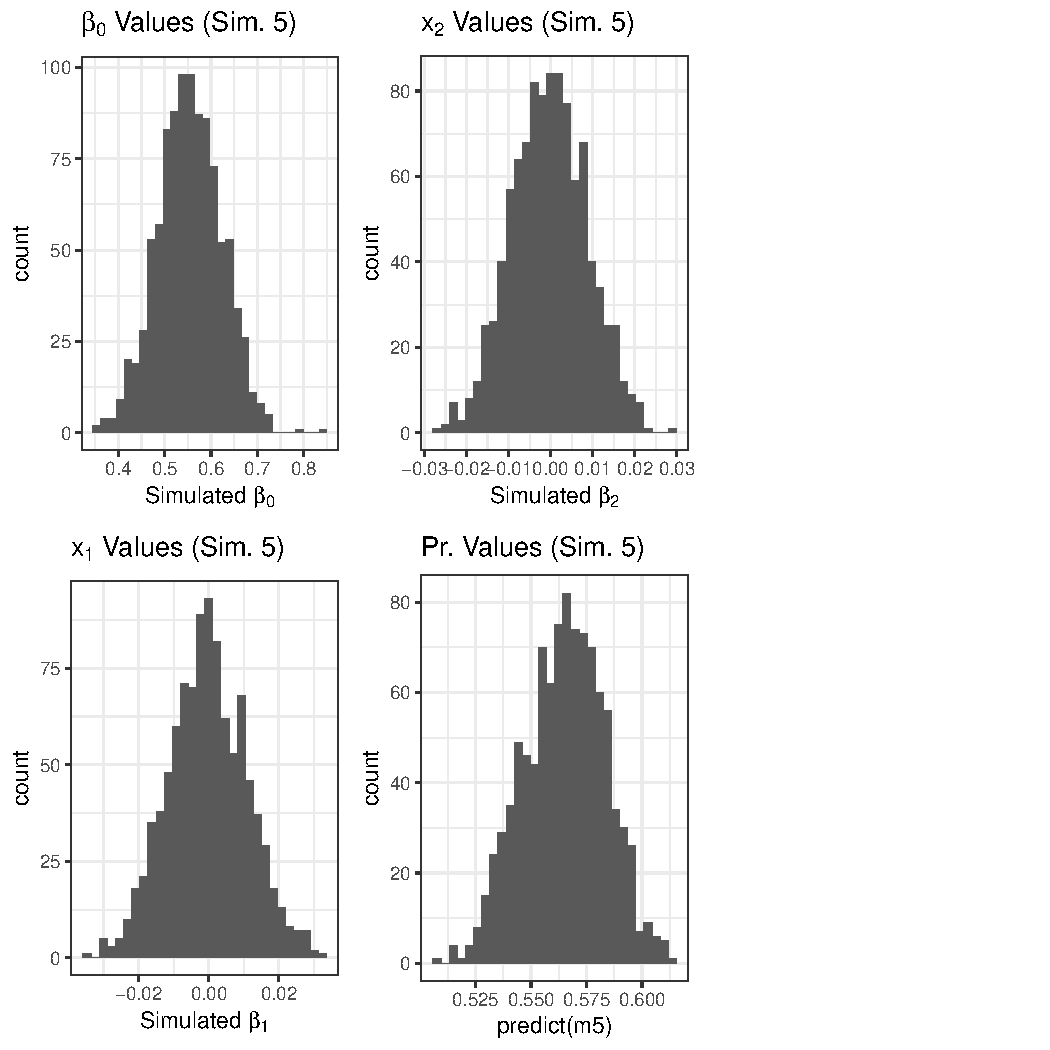
\includegraphics[width=5in]{figure/hiddenplotlineartologit-1} 
\begin{kframe}\begin{verbatim}
## [1] 2
\end{verbatim}
\end{kframe}
\end{knitrout}
\end{center}

Here we see the three estimates from our simulation and our model's prediction based upon the R \texttt{predict()} command. Our estimates are definately off and our predictions seem to be off because of this. Perhaps running a proper logit or probit model will help. We could run the same DGP but with the proper modeling using the \texttt{glm()} function, and the proper link function if we so desired.


\subsection{Penalized Regression: LASSO, Ridge, Elastic Net}

Let's use simulation to test out a few penalized regression models in R, starting with making a new DGP:

\begin{knitrout}
\definecolor{shadecolor}{rgb}{0.165, 0.169, 0.184}\color{fgcolor}\begin{kframe}
\begin{alltt}
\hlstd{> }\hlkwd{set.seed}\hlstd{(}\hlnum{12345}\hlstd{)}
\hlstd{> }\hlkwd{library}\hlstd{(caret)} \hlcom{#! for train() and Penalized Regression Functions}
\end{alltt}


{\ttfamily\noindent\color{warningcolor}{\#\# Warning: package 'caret' was built under R version 3.3.3}}\begin{alltt}
\hlstd{> }\hlkwd{library}\hlstd{(MASS)} \hlcom{# mvrnorm()}
\hlstd{> }\hlkwd{library}\hlstd{(Rlab)} \hlcom{# for rbern()}
\hlstd{> }\hlkwd{library}\hlstd{(glmnet)}
\end{alltt}


{\ttfamily\noindent\color{warningcolor}{\#\# Warning: package 'glmnet' was built under R version 3.3.3}}

{\ttfamily\noindent\itshape\color{messagecolor}{\#\# Loading required package: foreach}}

{\ttfamily\noindent\color{warningcolor}{\#\# Warning: package 'foreach' was built under R version 3.3.3}}

{\ttfamily\noindent\itshape\color{messagecolor}{\#\# Loaded glmnet 2.0-16}}\begin{alltt}
\hlstd{> }\hlstd{N} \hlkwb{<-} \hlnum{1000}
\hlstd{> }\hlstd{P} \hlkwb{<-} \hlnum{100}
\hlstd{> }\hlcom{# Wishart distribution for positive definite matricies}
\hlstd{> }\hlstd{Sigma} \hlkwb{<-} \hlkwd{rWishart}\hlstd{(}\hlkwc{n}\hlstd{=}\hlnum{1}\hlstd{,} \hlkwc{df}\hlstd{=P,} \hlkwc{Sigma}\hlstd{=}\hlkwd{diag}\hlstd{(P))[,,}\hlnum{1}\hlstd{]}
\hlstd{> }\hlstd{X} \hlkwb{<-} \hlkwd{mvrnorm}\hlstd{(N,} \hlkwd{runif}\hlstd{(P,} \hlopt{-}\hlnum{10}\hlstd{,} \hlnum{10}\hlstd{), Sigma)}
\hlstd{> }\hlstd{p} \hlkwb{<-} \hlkwd{rbern}\hlstd{(P,} \hlnum{0.1}\hlstd{)}
\hlstd{> }\hlstd{b} \hlkwb{<-} \hlstd{p} \hlopt{*} \hlkwd{rnorm}\hlstd{(P,} \hlnum{5}\hlstd{,} \hlnum{5}\hlstd{)} \hlopt{+} \hlstd{(}\hlnum{1}\hlopt{-}\hlstd{p)} \hlopt{*} \hlkwd{rnorm}\hlstd{(P,} \hlnum{0}\hlstd{,} \hlnum{0.1}\hlstd{)}
\hlstd{> }\hlstd{e} \hlkwb{<-} \hlkwd{rnorm}\hlstd{(N,} \hlnum{0}\hlstd{,} \hlkwc{sd}\hlstd{=}\hlkwd{sqrt}\hlstd{(}\hlnum{10}\hlstd{))}
\hlstd{> }\hlstd{y} \hlkwb{=} \hlstd{X}\hlopt\hlstd{b} \hlopt{+} \hlstd{e}
\hlstd{> }\hlstd{m1} \hlkwb{<-} \hlkwd{lm}\hlstd{(y}\hlopt{~}\hlstd{X)}
\hlstd{> }\hlcom{# Set data frame}
\hlstd{> }\hlstd{my_data} \hlkwb{=} \hlkwd{data.frame}\hlstd{(X,y)}
\end{alltt}
\end{kframe}
\end{knitrout}

Then we can use a few other functions to make a test set training set: \index{Test Set Training Set}

\begin{knitrout}
\definecolor{shadecolor}{rgb}{0.165, 0.169, 0.184}\color{fgcolor}\begin{kframe}
\begin{alltt}
\hlstd{> }\hlcom{## Test Set (20%); Training Set (80%)}
\hlstd{> }\hlcom{# Get 800 random index from y}
\hlstd{> }\hlstd{trainidx} \hlkwb{<-} \hlkwd{createDataPartition}\hlstd{(y,} \hlkwc{times} \hlstd{=} \hlnum{1}\hlstd{,} \hlkwc{p}\hlstd{=}\hlnum{.80}\hlstd{,} \hlkwc{list}\hlstd{=}\hlnum{FALSE}\hlstd{)}
\hlstd{> }\hlstd{trainy} \hlkwb{<-} \hlstd{y[trainidx]}  \hlcom{# Get traniing set index numbers; sample y's values}
\hlstd{> }\hlstd{testy} \hlkwb{<-} \hlstd{y[}\hlopt{-}\hlstd{trainidx]}  \hlcom{# Other 20% for test set (y)}
\hlstd{> }\hlstd{trainx} \hlkwb{<-} \hlstd{X[trainidx,]} \hlcom{# same for setting up X variable:}
\hlstd{> }\hlstd{testx} \hlkwb{<-} \hlstd{X[}\hlopt{-}\hlstd{trainidx,]}
\hlstd{> }
\hlstd{> }\hlcom{# Create Data Frames for these:}
\hlstd{> }\hlstd{train_data} \hlkwb{=} \hlkwd{data.frame}\hlstd{(trainx, trainy)}
\hlstd{> }\hlstd{test_data} \hlkwb{=} \hlkwd{data.frame}\hlstd{(testx, testy)}
\end{alltt}
\end{kframe}
\end{knitrout}

The idea here is to do data manipulation and all testing for significance just on a training set, using the test set to come in later to ``prove'' that everything is good-to-go independent of your training manipulations. It's a great practice, with many ways to do it in R; which will be showcased throughout this chapter. I prefer the \texttt{createDataPartition()} function myself.

Let us first plot the correlation between the true $\beta$ and our model's predicted $\beta$:

\begin{center}
\begin{knitrout}
\definecolor{shadecolor}{rgb}{0.165, 0.169, 0.184}\color{fgcolor}\begin{kframe}
\begin{alltt}
\hlstd{> }\hlkwd{library}\hlstd{(ggplot2)} \hlcom{# Graphing}
\hlstd{> }
\hlstd{> }\hlkwd{qplot}\hlstd{(b,} \hlkwd{coef}\hlstd{(m1)[}\hlopt{-}\hlnum{1}\hlstd{])}\hlopt{+}
\hlstd{+ }     \hlkwd{xlab}\hlstd{(} \hlkwd{expression}\hlstd{(}\hlkwd{paste}\hlstd{(}\hlstr{"True "} \hlstd{, beta)))}\hlopt{+}
\hlstd{+ }     \hlkwd{ylab}\hlstd{(} \hlkwd{expression}\hlstd{(}\hlkwd{paste}\hlstd{(}\hlstr{"Model "} \hlstd{,} \hlkwd{hat}\hlstd{(beta),} \hlstr{" Values"}\hlstd{)))}\hlopt{+}
\hlstd{+ }     \hlkwd{theme_bw}\hlstd{()}\hlopt{+}
\hlstd{+ }     \hlkwd{theme}\hlstd{(}\hlkwc{axis.text}\hlstd{=}\hlkwd{element_text}\hlstd{(}\hlkwc{size}\hlstd{=}\hlnum{12}\hlstd{),}
\hlstd{+ }           \hlkwc{axis.title}\hlstd{=}\hlkwd{element_text}\hlstd{(}\hlkwc{size}\hlstd{=}\hlnum{14}\hlstd{,}\hlkwc{face}\hlstd{=}\hlstr{"bold"}\hlstd{))}
\end{alltt}
\end{kframe}
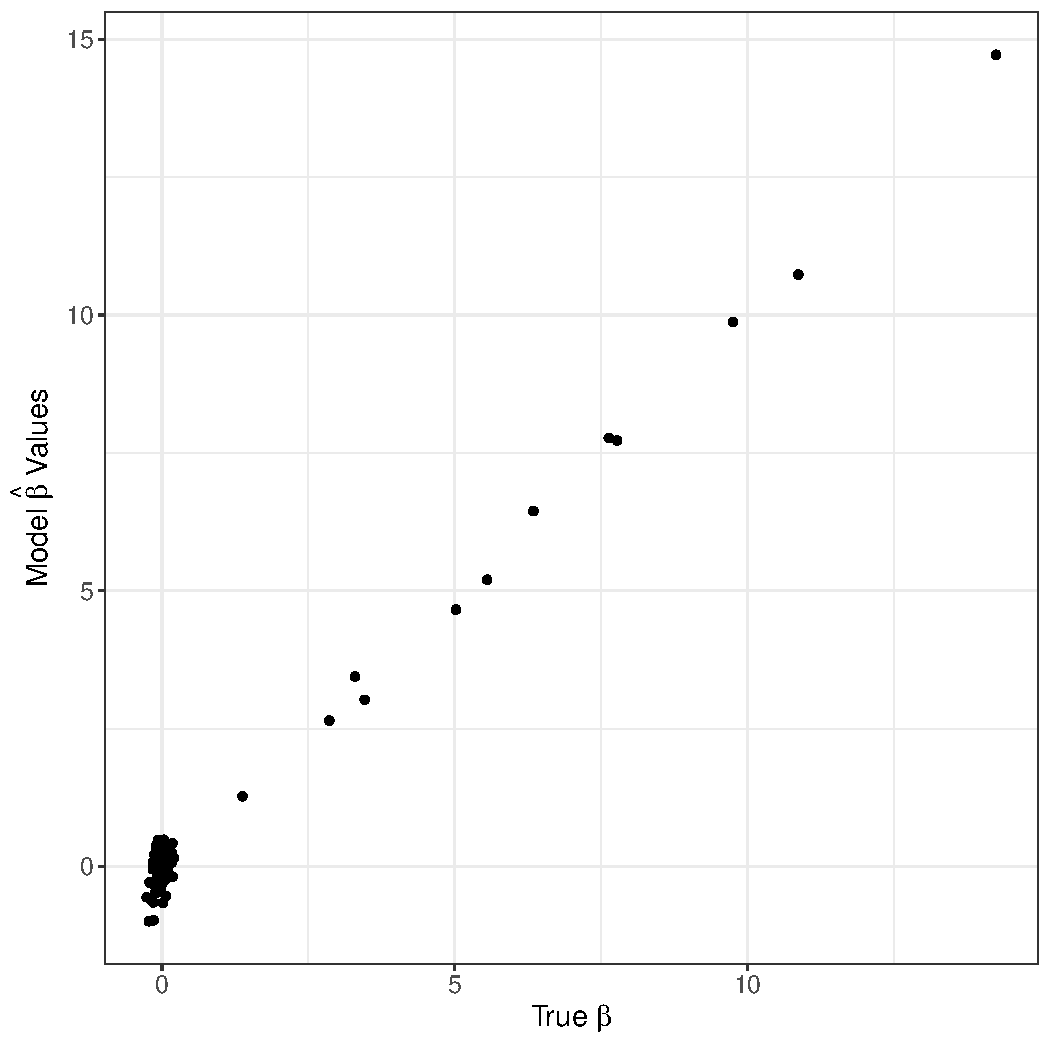
\includegraphics[width=5in]{figure/betabetatestPenRegress1-1} 

\end{knitrout}
\end{center}

These results make sense, most of our beta’s cluster with a mean around zero and some of our beta’s are outward with a mean around five and a larger standard deviation. Now, using our training data and leaving the test data aside, let’s run the same model within the training data, and examine the errors in a few different ways:

\begin{center}
\begin{knitrout}
\definecolor{shadecolor}{rgb}{0.165, 0.169, 0.184}\color{fgcolor}\begin{kframe}
\begin{alltt}
\hlstd{> }\hlcom{## Training Model:}
\hlstd{> }\hlstd{trainmod} \hlkwb{<-} \hlkwd{lm}\hlstd{(train_data}\hlopt{$}\hlstd{trainy} \hlopt{~} \hlstd{trainx,} \hlkwc{data} \hlstd{= train_data)}
\hlstd{> }\hlcom{# summary(trainmod) # Check that this makes sense}
\hlstd{> }
\hlstd{> }\hlstd{error} \hlkwb{<-} \hlstd{train_data}\hlopt{$}\hlstd{trainy} \hlopt{-} \hlkwd{predict}\hlstd{(trainmod)}
\hlstd{> }\hlcom{# head(error) # Check this makes sense}
\hlstd{> }
\hlstd{> }\hlcom{# Ideally we want normality here, mean zero}
\hlstd{> }\hlkwd{qplot}\hlstd{(error,} \hlkwc{bins}\hlstd{=}\hlnum{50}\hlstd{,} \hlkwc{fill}\hlstd{=}\hlkwd{I}\hlstd{(}\hlstr{"grey10"}\hlstd{))}\hlopt{+}
\hlstd{+ }     \hlkwd{xlab}\hlstd{(} \hlstr{"Model Errors"}\hlstd{)}\hlopt{+}
\hlstd{+ }     \hlkwd{ylab}\hlstd{(} \hlstr{"Count"}\hlstd{)}\hlopt{+}
\hlstd{+ }     \hlkwd{theme_bw}\hlstd{()}\hlopt{+}
\hlstd{+ }     \hlkwd{theme}\hlstd{(}\hlkwc{axis.text}\hlstd{=}\hlkwd{element_text}\hlstd{(}\hlkwc{size}\hlstd{=}\hlnum{12}\hlstd{),}
\hlstd{+ }           \hlkwc{axis.title}\hlstd{=}\hlkwd{element_text}\hlstd{(}\hlkwc{size}\hlstd{=}\hlnum{14}\hlstd{))}
\end{alltt}
\end{kframe}
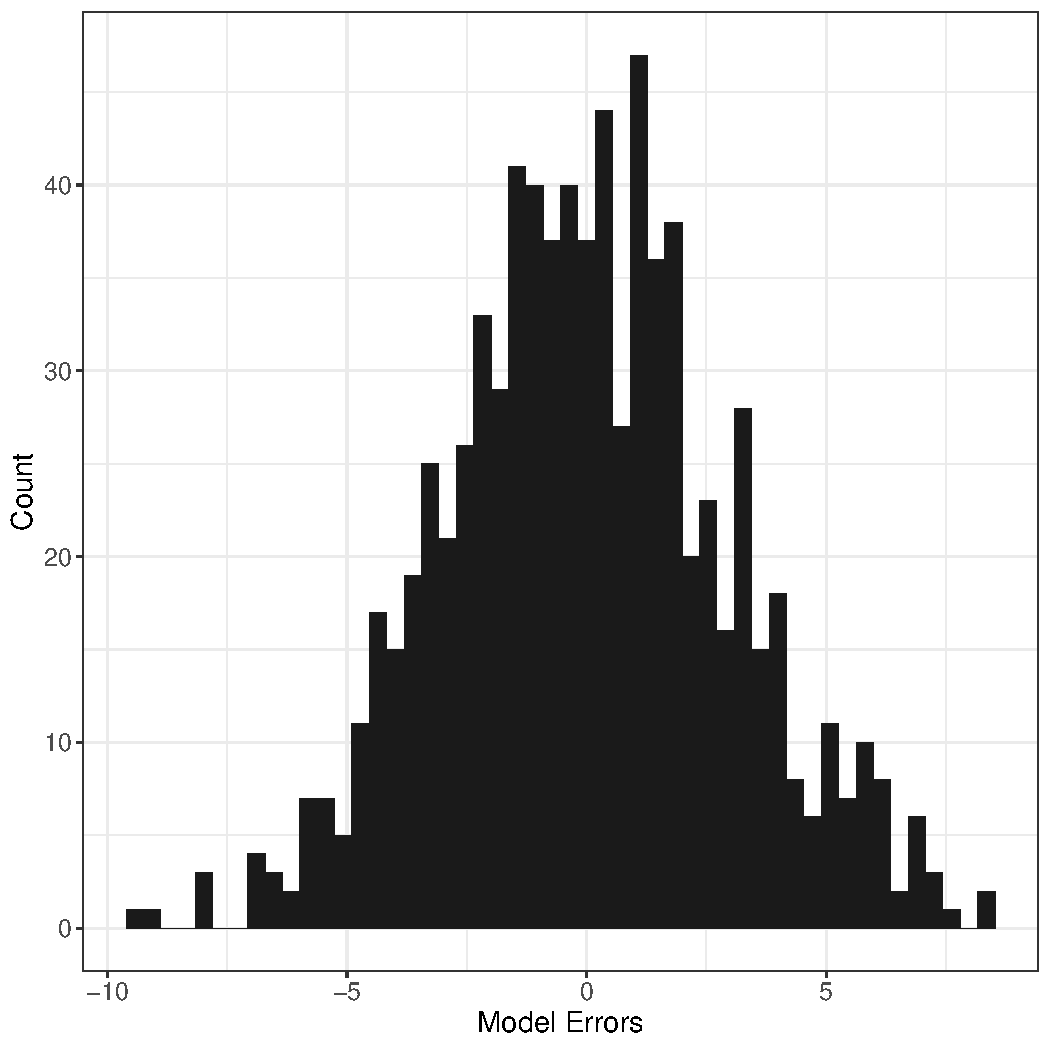
\includegraphics[width=5in]{figure/examineerrorsML-1} 

\end{knitrout}
\end{center}

\begin{knitrout}
\definecolor{shadecolor}{rgb}{0.165, 0.169, 0.184}\color{fgcolor}\begin{kframe}
\begin{alltt}
\hlstd{> }\hlcom{## Root Mean Squred Error}
\hlstd{> }\hlkwd{sqrt}\hlstd{(}\hlkwd{mean}\hlstd{(error}\hlopt{^}\hlnum{2}\hlstd{))}
\end{alltt}
\begin{verbatim}
## [1] 3.039912
\end{verbatim}
\begin{alltt}
\hlstd{> }\hlcom{## [1] 3.039912}
\hlstd{> }
\hlstd{> }\hlcom{## Mean Aboslute Error}
\hlstd{> }\hlkwd{mean}\hlstd{(}\hlkwd{abs}\hlstd{(error))}
\end{alltt}
\begin{verbatim}
## [1] 2.415841
\end{verbatim}
\begin{alltt}
\hlstd{> }\hlcom{## [1] 2.415841}
\end{alltt}
\end{kframe}
\end{knitrout}

Using just our training data with the linear model we see our root mean squared error and mean absolute error are about around 3, pretty low. More intutitvely, our errors when plotted are normally distributed with a mean of zero. We can revisit this with a LASSO and Ridge regression to penalize us for having so many parameters for so few observations. Using penalized regression is especially helpful with models that have a large number of predictors relative to our sample size. The ``elastic net'' is particularly useful because it ``switches'' between two other penalties (using $\alpha$), the ``LASSO'' (Least Aboslute Shrinkage and Selection Operator uses a squared transformation) and “Ridge” (using the absolute value of our coefficents), applying both of these in an ever-checking gradient descent down our distribution to the point of least error. Ideally we would like a smooth distribution in this process instead of quick-changing erratic distribution and the elastic net provides the previously mentioned functions to accomplish this via the transformation of our coecents as they travel farther away from zero.\index{LASSO} \index{Ridge} \index{Elastic Net}

Let's begin with the LASSO:

\begin{center}
\begin{knitrout}
\definecolor{shadecolor}{rgb}{0.165, 0.169, 0.184}\color{fgcolor}\begin{kframe}
\begin{alltt}
\hlstd{> }\hlcom{# Remember our training data frame:}
\hlstd{> }\hlstd{train_data} \hlkwb{=} \hlkwd{data.frame}\hlstd{(trainx, trainy)}
\hlstd{> }
\hlstd{> }\hlstd{mod_lasso} \hlkwb{=} \hlkwd{train}\hlstd{(trainy}\hlopt{~}\hlstd{.,} \hlkwc{method}\hlstd{=}\hlstr{"glmnet"}\hlstd{,}\hlcom{# formula and method}
\hlstd{+ }     \hlkwc{tuneGrid}\hlstd{=}\hlkwd{expand.grid}\hlstd{(}\hlkwc{alpha} \hlstd{=} \hlnum{0}\hlstd{,} \hlcom{# alpha=0 is the LASSO}
\hlstd{+ }               \hlkwc{lambda} \hlstd{=} \hlkwd{seq}\hlstd{(}\hlnum{0}\hlstd{,}\hlnum{100}\hlstd{,}\hlnum{1}\hlstd{)),} \hlcom{#gradient descent to zero}
\hlstd{+ }     \hlkwc{data} \hlstd{= train_data,}
\hlstd{+ }     \hlkwc{preProcess} \hlstd{=} \hlkwd{c}\hlstd{(}\hlstr{"center"}\hlstd{),}\hlcom{# centering standardization of points}
\hlstd{+ }     \hlkwc{trControl} \hlstd{=} \hlkwd{trainControl}\hlstd{(}\hlkwc{method}\hlstd{=}\hlstr{"cv"}\hlstd{,}\hlkwc{number}\hlstd{=}\hlnum{2}\hlstd{,} \hlkwc{search}\hlstd{=}\hlstr{"grid"}\hlstd{))}
\hlstd{> }\hlcom{# "trainControl" sets a resampling method per a "search" parameter grid}
\hlstd{> }\hlcom{# mod_lasso ## final values were around lambda = 14 using RMSE}
\hlstd{> }
\hlstd{> }\hlcom{## Narrowing lambda sequence closer to what the lambda reported earlier:}
\hlstd{> }\hlstd{mod_lasso} \hlkwb{=} \hlkwd{train}\hlstd{(trainy}\hlopt{~}\hlstd{.,} \hlkwc{method} \hlstd{=} \hlstr{"glmnet"}\hlstd{,}
\hlstd{+ }     \hlkwc{tuneGrid} \hlstd{=} \hlkwd{expand.grid}\hlstd{(}\hlkwc{alpha} \hlstd{=} \hlnum{0}\hlstd{,}
\hlstd{+ }     \hlcom{# *setting bounds closer around 14; smaller "steps" (0.01)}
\hlstd{+ }                         \hlkwc{lambda} \hlstd{=} \hlkwd{seq}\hlstd{(}\hlnum{0}\hlstd{,}\hlnum{40}\hlstd{,}\hlnum{0.01}\hlstd{)),}
\hlstd{+ }     \hlkwc{data} \hlstd{= train_data,}
\hlstd{+ }     \hlkwc{preProcess} \hlstd{=} \hlkwd{c}\hlstd{(}\hlstr{"center"}\hlstd{),}
\hlstd{+ }     \hlkwc{trControl} \hlstd{=} \hlkwd{trainControl}\hlstd{(}\hlkwc{method}\hlstd{=}\hlstr{"cv"}\hlstd{,}\hlkwc{number}\hlstd{=}\hlnum{2}\hlstd{,} \hlkwc{search}\hlstd{=}\hlstr{"grid"}\hlstd{))}
\hlstd{> }     \hlcom{# mod_lasso ## Narrowing in, we found a new best lambda of around 14.5!}
\hlstd{> }
\hlstd{> }\hlcom{## Predictions:}
\hlstd{> }\hlstd{yhat} \hlkwb{=} \hlkwd{predict}\hlstd{(mod_lasso)}
\hlstd{> }\hlcom{# alpha allows transparent points to see density}
\hlstd{> }\hlkwd{qplot}\hlstd{(trainy, yhat,} \hlkwc{alpha}\hlstd{=}\hlkwd{I}\hlstd{(}\hlnum{0.25}\hlstd{))}\hlopt{+}
\hlstd{+ }     \hlkwd{xlab}\hlstd{(} \hlkwd{expression}\hlstd{(}\hlkwd{paste}\hlstd{(}\hlstr{"Training "}\hlstd{, y)))}\hlopt{+}
\hlstd{+ }     \hlkwd{ylab}\hlstd{(} \hlkwd{expression}\hlstd{(}\hlkwd{paste}\hlstd{(}\hlstr{"Ridge "}\hlstd{,} \hlkwd{hat}\hlstd{(y))))}\hlopt{+}
\hlstd{+ }     \hlkwd{theme_bw}\hlstd{()}\hlopt{+}
\hlstd{+ }     \hlkwd{theme}\hlstd{(}\hlkwc{axis.text} \hlstd{=} \hlkwd{element_text}\hlstd{(}\hlkwc{size}\hlstd{=}\hlnum{12}\hlstd{),}
\hlstd{+ }          \hlkwc{axis.title} \hlstd{=} \hlkwd{element_text}\hlstd{(}\hlkwc{size}\hlstd{=}\hlnum{14}\hlstd{))}
\end{alltt}
\end{kframe}
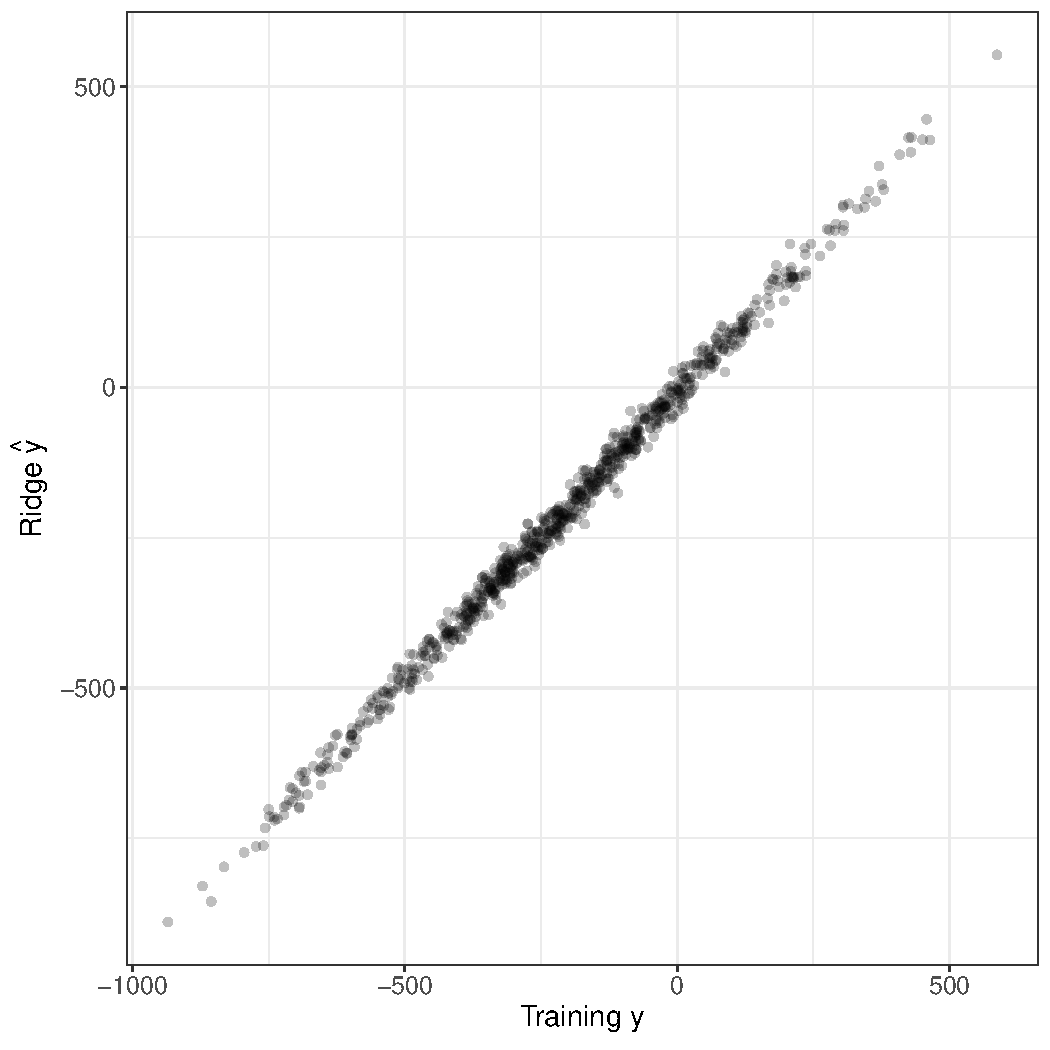
\includegraphics[width=5in]{figure/LASSO1ML-1} 

\end{knitrout}
\end{center}
\index{GGplot}

\begin{center}
\begin{knitrout}
\definecolor{shadecolor}{rgb}{0.165, 0.169, 0.184}\color{fgcolor}\begin{kframe}
\begin{alltt}
\hlstd{> }\hlcom{# best values using best lambda:}
\hlstd{> }\hlstd{lasso_beta} \hlkwb{=} \hlkwd{coef}\hlstd{(mod_lasso}\hlopt{$}\hlstd{finalModel, mod_lasso}\hlopt{$}\hlstd{bestTune}\hlopt{$}\hlstd{lambda)}
\hlstd{> }
\hlstd{> }\hlkwd{qplot}\hlstd{(b, lasso_beta[}\hlopt{-}\hlnum{1}\hlstd{])}\hlopt{+} \hlcom{# removing intercept}
\hlstd{+ }     \hlkwd{xlab}\hlstd{(} \hlkwd{expression}\hlstd{(}\hlkwd{paste}\hlstd{(}\hlstr{"True "}\hlstd{, beta)))}\hlopt{+}
\hlstd{+ }     \hlkwd{ylab}\hlstd{(} \hlkwd{expression}\hlstd{(}\hlkwd{paste}\hlstd{(}\hlstr{"LASSO "}\hlstd{, beta)))}\hlopt{+}
\hlstd{+ }     \hlkwd{theme_bw}\hlstd{()}\hlopt{+}
\hlstd{+ }     \hlkwd{theme}\hlstd{(}\hlkwc{axis.text} \hlstd{=} \hlkwd{element_text}\hlstd{(}\hlkwc{size}\hlstd{=}\hlnum{12}\hlstd{),}
\hlstd{+ }          \hlkwc{axis.title} \hlstd{=} \hlkwd{element_text}\hlstd{(}\hlkwc{size}\hlstd{=}\hlnum{14}\hlstd{))}
\end{alltt}
\end{kframe}
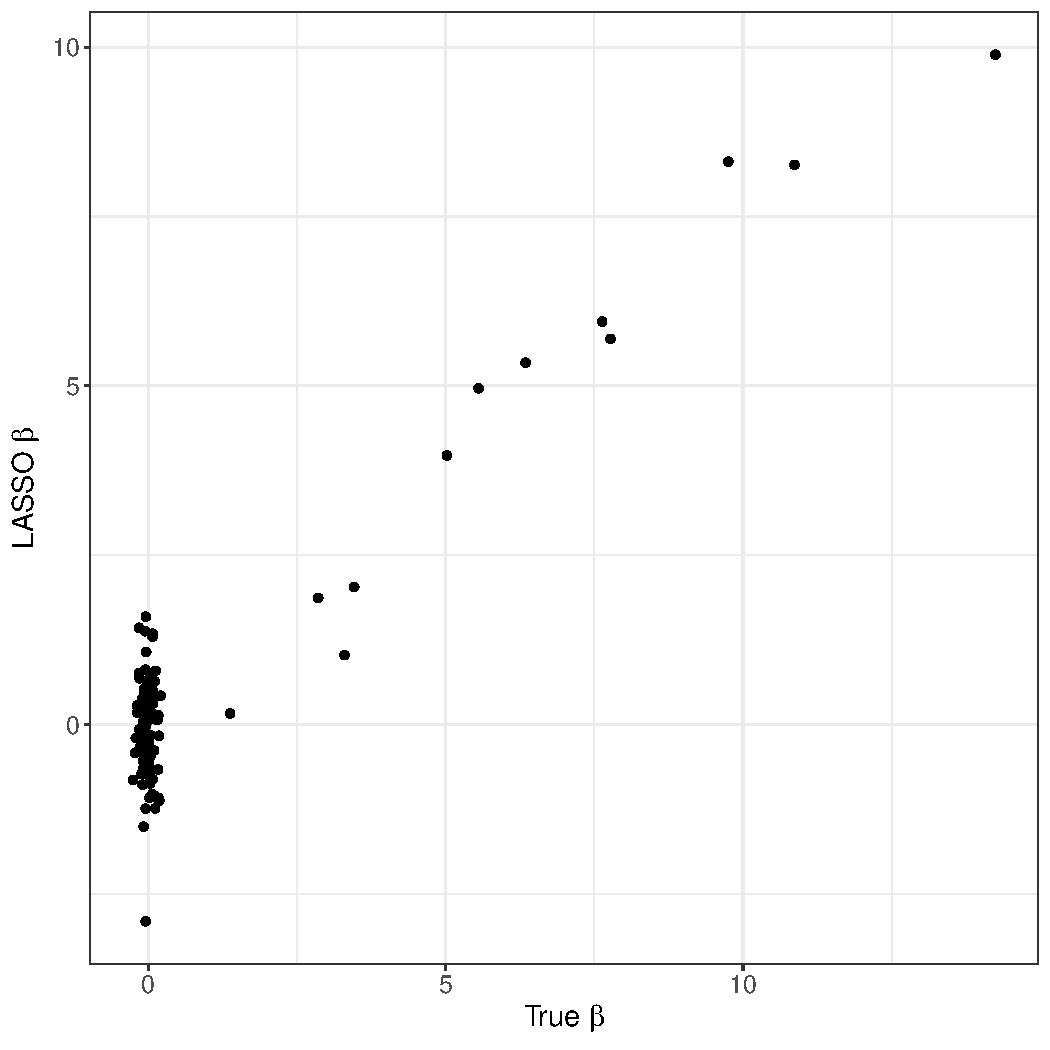
\includegraphics[width=5in]{figure/LASSOvaluesML1-1} 

\end{knitrout}
\end{center}

What this tells us is that our predicted values from the LASSO model does well with our training $y$ data. Specifcally, in the first figure we see that our training dependent variable and our penalized LASSO predictions match with each other positively. In the second figure, we see our actual beta’s more accurately plotted in conjunction with the LASSO’s best fit betas.
Similarly, let’s see how the Ridge and elastic net’s hold up:

\begin{center}
\begin{knitrout}
\definecolor{shadecolor}{rgb}{0.165, 0.169, 0.184}\color{fgcolor}\begin{kframe}
\begin{alltt}
\hlstd{> }\hlcom{## Running Ridge:}
\hlstd{> }\hlstd{mod_ridge} \hlkwb{=} \hlkwd{train}\hlstd{(trainy}\hlopt{~}\hlstd{.,} \hlkwc{method}\hlstd{=}\hlstr{"glmnet"}\hlstd{,}
\hlstd{+ }          \hlkwc{tuneGrid}\hlstd{=}\hlkwd{expand.grid}\hlstd{(}\hlkwc{alpha}\hlstd{=}\hlnum{1}\hlstd{,}
\hlstd{+ }               \hlkwc{lambda}\hlstd{=}\hlkwd{seq}\hlstd{(}\hlnum{0}\hlstd{,}\hlnum{10}\hlstd{,}\hlnum{0.01}\hlstd{)),}
\hlstd{+ }          \hlkwc{data}\hlstd{=train_data,}
\hlstd{+ }          \hlkwc{preProcess}\hlstd{=}\hlkwd{c}\hlstd{(}\hlstr{"center"}\hlstd{),}
\hlstd{+ }          \hlkwc{trControl}\hlstd{=}\hlkwd{trainControl}\hlstd{(}\hlkwc{method}\hlstd{=}\hlstr{"cv"}\hlstd{,}\hlkwc{number}\hlstd{=}\hlnum{2}\hlstd{,} \hlkwc{search}\hlstd{=}\hlstr{"grid"}\hlstd{))}
\hlstd{> }\hlcom{# Best lambda (RMSE) is 1.01}
\hlstd{> }
\hlstd{> }\hlstd{mod_ridge} \hlkwb{=} \hlkwd{train}\hlstd{(trainy}\hlopt{~}\hlstd{.,} \hlkwc{method}\hlstd{=}\hlstr{"glmnet"}\hlstd{,}
\hlstd{+ }          \hlkwc{tuneGrid}\hlstd{=}\hlkwd{expand.grid}\hlstd{(}\hlkwc{alpha}\hlstd{=}\hlnum{1}\hlstd{,}
\hlstd{+ }               \hlkwc{lambda}\hlstd{=}\hlkwd{seq}\hlstd{(}\hlnum{0}\hlstd{,}\hlnum{3}\hlstd{,}\hlnum{0.01}\hlstd{)),}
\hlstd{+ }          \hlkwc{data}\hlstd{=train_data,}
\hlstd{+ }          \hlkwc{preProcess}\hlstd{=}\hlkwd{c}\hlstd{(}\hlstr{"center"}\hlstd{),}
\hlstd{+ }          \hlkwc{trControl}\hlstd{=}\hlkwd{trainControl}\hlstd{(}\hlkwc{method}\hlstd{=}\hlstr{"cv"}\hlstd{,}\hlkwc{number}\hlstd{=}\hlnum{2}\hlstd{,} \hlkwc{search}\hlstd{=}\hlstr{"grid"}\hlstd{))}
\hlstd{> }
\hlstd{> }\hlcom{# New best lambda of .94}
\hlstd{> }\hlstd{yhat} \hlkwb{=} \hlkwd{predict}\hlstd{(mod_ridge)}
\hlstd{> }
\hlstd{> }\hlkwd{qplot}\hlstd{(trainy, yhat,} \hlkwc{alpha}\hlstd{=}\hlkwd{I}\hlstd{(}\hlnum{0.25}\hlstd{))}\hlopt{+}
\hlstd{+ }     \hlkwd{xlab}\hlstd{(} \hlkwd{expression}\hlstd{(}\hlkwd{paste}\hlstd{(}\hlstr{"Training "}\hlstd{, y)))}\hlopt{+}
\hlstd{+ }     \hlkwd{ylab}\hlstd{(} \hlkwd{expression}\hlstd{(}\hlkwd{paste}\hlstd{(}\hlstr{"Ridge "}\hlstd{,} \hlkwd{hat}\hlstd{(y))))}\hlopt{+}
\hlstd{+ }     \hlkwd{theme_bw}\hlstd{()}\hlopt{+}
\hlstd{+ }     \hlkwd{theme}\hlstd{(}\hlkwc{axis.text} \hlstd{=} \hlkwd{element_text}\hlstd{(}\hlkwc{size}\hlstd{=}\hlnum{12}\hlstd{),}
\hlstd{+ }          \hlkwc{axis.title} \hlstd{=} \hlkwd{element_text}\hlstd{(}\hlkwc{size}\hlstd{=}\hlnum{14}\hlstd{))}
\end{alltt}
\end{kframe}
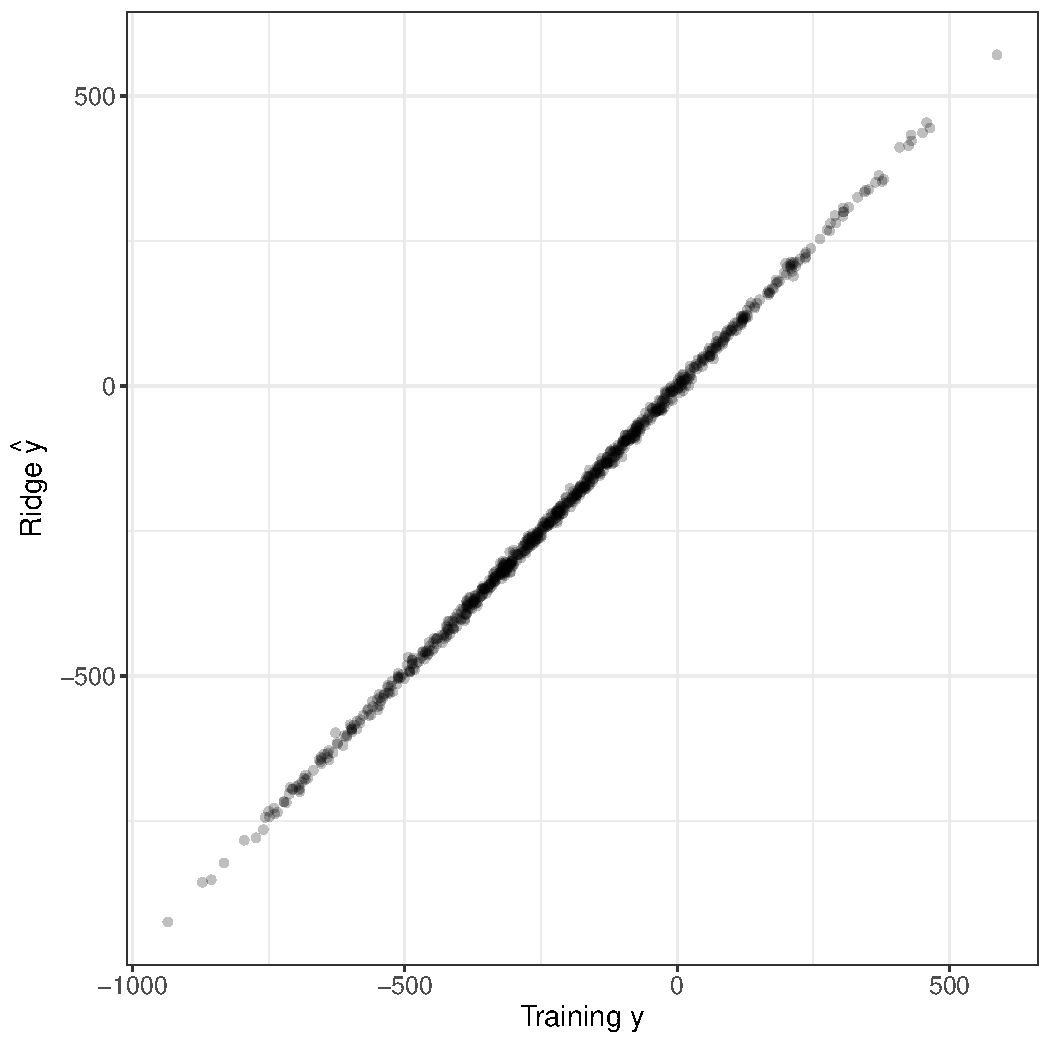
\includegraphics[width=5in]{figure/RidgeNetML1-1} 

\end{knitrout}
\end{center}

\begin{center}
\begin{knitrout}
\definecolor{shadecolor}{rgb}{0.165, 0.169, 0.184}\color{fgcolor}\begin{kframe}
\begin{alltt}
\hlstd{> }\hlstd{ridge_beta} \hlkwb{=} \hlkwd{coef}\hlstd{(mod_ridge}\hlopt{$}\hlstd{finalModel, mod_ridge}\hlopt{$}\hlstd{bestTune}\hlopt{$}\hlstd{lambda)}
\hlstd{> }
\hlstd{> }\hlkwd{qplot}\hlstd{(b, ridge_beta[}\hlopt{-}\hlnum{1}\hlstd{])}\hlopt{+}
\hlstd{+ }     \hlkwd{xlab}\hlstd{(} \hlkwd{expression}\hlstd{(}\hlkwd{paste}\hlstd{(}\hlstr{"True "}\hlstd{, beta)))}\hlopt{+}
\hlstd{+ }     \hlkwd{ylab}\hlstd{(} \hlkwd{expression}\hlstd{(}\hlkwd{paste}\hlstd{(}\hlstr{"Ridge "}\hlstd{, beta)))}\hlopt{+}
\hlstd{+ }     \hlkwd{theme_bw}\hlstd{()}\hlopt{+}
\hlstd{+ }     \hlkwd{theme}\hlstd{(}\hlkwc{axis.text} \hlstd{=} \hlkwd{element_text}\hlstd{(}\hlkwc{size}\hlstd{=}\hlnum{12}\hlstd{),}
\hlstd{+ }          \hlkwc{axis.title} \hlstd{=} \hlkwd{element_text}\hlstd{(}\hlkwc{size}\hlstd{=}\hlnum{14}\hlstd{))}
\end{alltt}
\end{kframe}
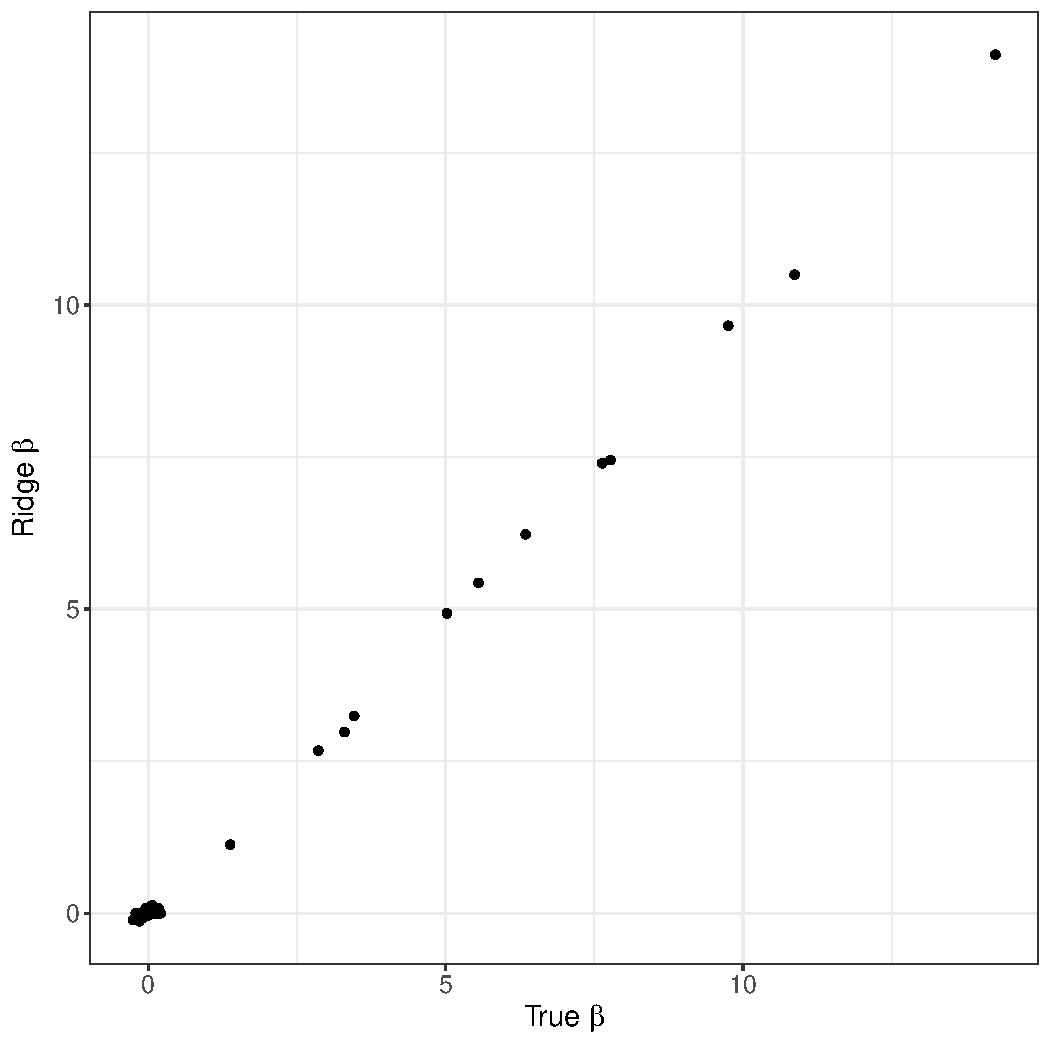
\includegraphics[width=5in]{figure/Ridgenet2MLthing-1} 

\end{knitrout}
\end{center}

Our ridge regression shows less variability, our training set $y$ values and ridge predicted values are more tightly linear, and there is less variability in our comparative $\beta$ values in the plot above. This is interesting and is perhaps explained in the difference between the mathematical formula between Ridge and LASSO themselves (letting $\lambda$ control the amount of regulation in gradient descent):

\

\textbf{Ridge:} ($\alpha = 0$ )

\begin{equation}
\lambda \sum_{j=1}^{p} \left[ \frac{1}{2} (1- \alpha) \beta^2 \right]
\end{equation}

\textbf{LASSO:} ($\alpha = 1$ )

\begin{equation}
\lambda \sum_{j=1}^{p} (\alpha) | \beta_j |
\end{equation}

We seek a set of sparse solutions because we beleive that many of our 100 $\beta_j$ paramenters should be zero; a large enough $\lambda$ will set these exactly or near zero for us! We saw our LASSO $\lambda$ values become higher than our Ridge $\lambda$ values; this is because, unlike Ridge, our $\beta_{\lambda}^{\text{lass}}}$ lasso values have no closed form – allowing more varriance. A third potential option is to allow our alpha parameter varry between zero and one eectively using both of these penalties and giving us the elastic net (litterally just adding LASSO and Ridge).

\

\textbf{Elastic Net:} ($0 < \alpha < 1$)

\begin{equation}
\lambda \sum_{j=1}^{p} \left[ \frac{1}{2} (1- \alpha) \beta^2 \right] + \lambda \sum_{j=1}^{p} (\alpha) | \beta_j |
\end{equation}



\begin{knitrout}
\definecolor{shadecolor}{rgb}{0.165, 0.169, 0.184}\color{fgcolor}\begin{kframe}
\begin{alltt}
\hlstd{> }\hlcom{## Elastic Net:}
\hlstd{> }\hlstd{mod_enet} \hlkwb{=} \hlkwd{train}\hlstd{(trainy}\hlopt{~}\hlstd{.,} \hlkwc{method} \hlstd{=} \hlstr{"glmnet"}\hlstd{,}
\hlstd{+ }            \hlkwc{tuneGrid} \hlstd{=} \hlkwd{expand.grid}\hlstd{(}\hlkwc{alpha} \hlstd{=} \hlkwd{seq}\hlstd{(}\hlnum{0}\hlstd{,} \hlnum{1}\hlstd{,} \hlnum{0.1}\hlstd{),}
\hlstd{+ }                                   \hlkwc{lambda} \hlstd{=} \hlkwd{seq}\hlstd{(}\hlnum{0}\hlstd{,} \hlnum{100}\hlstd{,} \hlnum{1}\hlstd{)),}
\hlstd{+ }            \hlkwc{data} \hlstd{= train_data,}
\hlstd{+ }            \hlkwc{preProcess} \hlstd{=} \hlkwd{c}\hlstd{(}\hlstr{"center"}\hlstd{),}
\hlstd{+ }            \hlkwc{trControl} \hlstd{=} \hlkwd{trainControl}\hlstd{(}\hlkwc{method}\hlstd{=}\hlstr{"cv"}\hlstd{,} \hlkwc{number}\hlstd{=}\hlnum{2}\hlstd{,} \hlkwc{search}\hlstd{=}\hlstr{"grid"}\hlstd{))}
\hlstd{> }\hlcom{# alpha used was .9 and lambda ended up being 1.}
\end{alltt}
\end{kframe}
\end{knitrout}

This elastic net will give us similarlly better results with a varrying $\alpha$ along with it. However, these models work best for when we have data with many parameters, here we have only started with 100 (``only''). Let's ramp up the number of perameters (P) and really put these models to the test. I'll repost the DGP in full.

\begin{knitrout}
\definecolor{shadecolor}{rgb}{0.165, 0.169, 0.184}\color{fgcolor}\begin{kframe}
\begin{alltt}
\hlstd{> }\hlstd{N} \hlkwb{<-} \hlnum{1000}
\hlstd{> }\hlstd{P} \hlkwb{<-} \hlnum{1500} \hlcom{# Note this change}
\hlstd{> }\hlstd{Sigma} \hlkwb{<-} \hlkwd{rWishart}\hlstd{(}\hlkwc{n}\hlstd{=}\hlnum{1}\hlstd{,} \hlkwc{df}\hlstd{=P,} \hlkwc{Sigma}\hlstd{=}\hlkwd{diag}\hlstd{(P))[,,}\hlnum{1}\hlstd{]}
\hlstd{> }\hlstd{X} \hlkwb{<-} \hlkwd{mvrnorm}\hlstd{(N,} \hlkwd{runif}\hlstd{(P,} \hlopt{-}\hlnum{10}\hlstd{,} \hlnum{10}\hlstd{), Sigma)}
\hlstd{> }\hlstd{p} \hlkwb{<-} \hlkwd{rbern}\hlstd{(P,} \hlnum{0.1}\hlstd{)}
\hlstd{> }\hlstd{b} \hlkwb{<-} \hlstd{p} \hlopt{*} \hlkwd{rnorm}\hlstd{(P,} \hlnum{5}\hlstd{,} \hlnum{5}\hlstd{)} \hlopt{+} \hlstd{(}\hlnum{1}\hlopt{-}\hlstd{p)} \hlopt{*} \hlkwd{rnorm}\hlstd{(P,} \hlnum{0}\hlstd{,} \hlnum{0.1}\hlstd{)}
\hlstd{> }\hlstd{e} \hlkwb{<-} \hlkwd{rnorm}\hlstd{(N,} \hlnum{0}\hlstd{,} \hlkwc{sd}\hlstd{=}\hlkwd{sqrt}\hlstd{(}\hlnum{10}\hlstd{))}
\hlstd{> }\hlstd{y} \hlkwb{=} \hlstd{X}\hlopt\hlstd{b} \hlopt{+} \hlstd{e}
\hlstd{> }\hlstd{m1} \hlkwb{<-} \hlkwd{lm}\hlstd{(y}\hlopt{~}\hlstd{X)}
\hlstd{> }\hlstd{my_data} \hlkwb{=} \hlkwd{data.frame}\hlstd{(X,y)}
\end{alltt}
\end{kframe}
\end{knitrout}

With this DGP, let's see how our regular linear model holds up graphically:

\begin{knitrout}
\definecolor{shadecolor}{rgb}{0.165, 0.169, 0.184}\color{fgcolor}\begin{kframe}
\begin{alltt}
\hlstd{> }\hlcom{## Problematic:}
\hlstd{> }\hlkwd{qplot}\hlstd{(b,} \hlkwd{coef}\hlstd{(m1)[}\hlopt{-}\hlnum{1}\hlstd{],} \hlkwc{alpha}\hlstd{=}\hlkwd{I}\hlstd{(}\hlnum{0.25}\hlstd{))}\hlopt{+}
\hlstd{+ }     \hlkwd{xlab}\hlstd{(} \hlkwd{expression}\hlstd{(}\hlkwd{paste}\hlstd{(}\hlstr{"True "} \hlstd{, beta)))}\hlopt{+}
\hlstd{+ }     \hlkwd{ylab}\hlstd{(} \hlkwd{expression}\hlstd{(}\hlkwd{paste}\hlstd{(}\hlstr{"Model "} \hlstd{,} \hlkwd{hat}\hlstd{(beta),} \hlstr{" Values"}\hlstd{)))}\hlopt{+}
\hlstd{+ }     \hlkwd{theme_bw}\hlstd{()}\hlopt{+}
\hlstd{+ }     \hlkwd{theme}\hlstd{(}\hlkwc{axis.text} \hlstd{=} \hlkwd{element_text}\hlstd{(}\hlkwc{size}\hlstd{=}\hlnum{12}\hlstd{),}
\hlstd{+ }          \hlkwc{axis.title} \hlstd{=} \hlkwd{element_text}\hlstd{(}\hlkwc{size}\hlstd{=}\hlnum{14}\hlstd{))}
\end{alltt}


{\ttfamily\noindent\color{warningcolor}{\#\# Warning: Removed 501 rows containing missing values (geom\_point).}}\end{kframe}
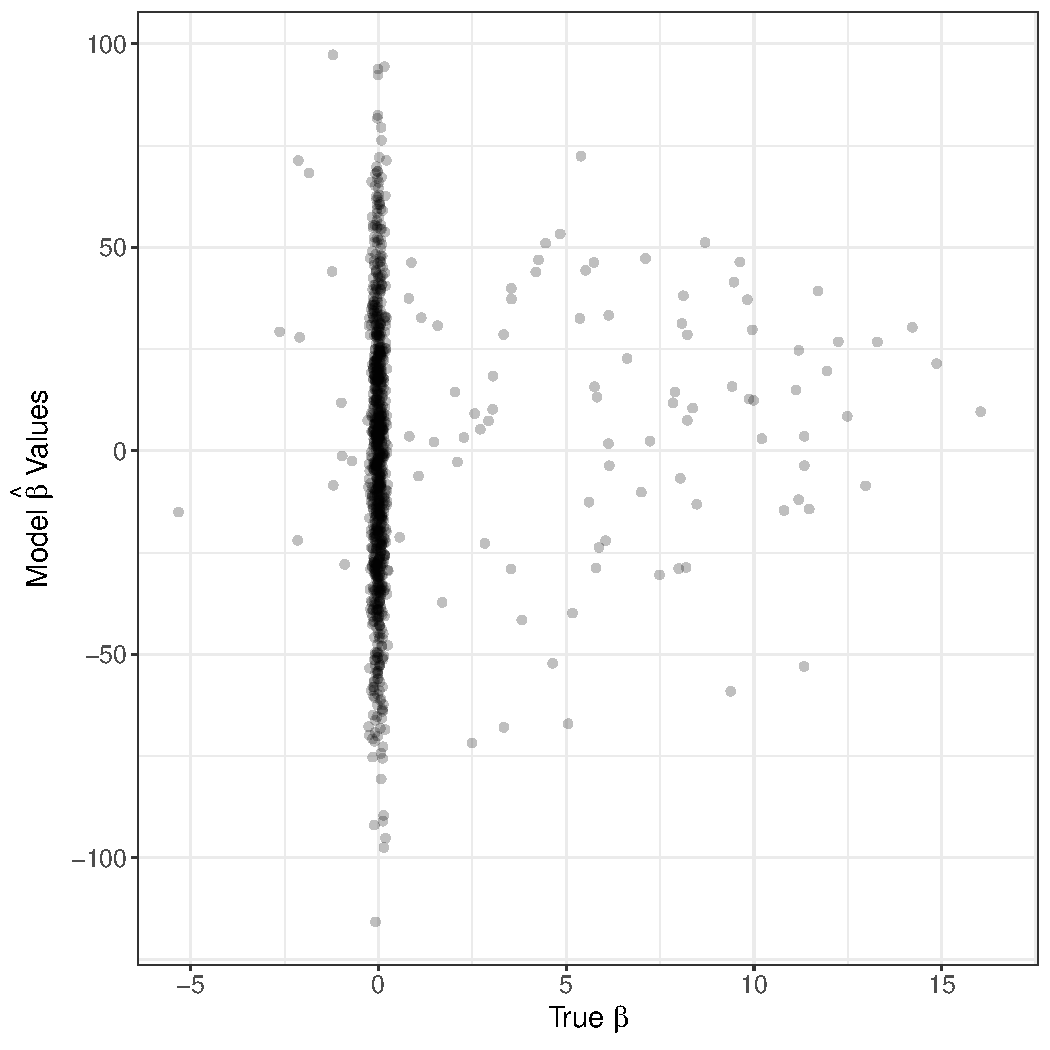
\includegraphics[width=5in]{figure/lmoutputML2-1} 

\end{knitrout}

We see quite a bit of noise, also our results will be outrageously significant because we are not penalizing ourselves for multiple parameters unless we are using the AIC and BIC. Now let's see if the elastic net does any better given the larger number of parameters. We'll start by chopping up the data into a testing set and a training set. \index{Test Set Training Set}

\begin{knitrout}
\definecolor{shadecolor}{rgb}{0.165, 0.169, 0.184}\color{fgcolor}\begin{kframe}
\begin{alltt}
\hlstd{> }\hlcom{# Test Set; Training Set (20% and 80% again)}
\hlstd{> }\hlstd{trainidx} \hlkwb{<-} \hlkwd{createDataPartition}\hlstd{(y,} \hlkwc{times} \hlstd{=} \hlnum{1}\hlstd{,} \hlkwc{p}\hlstd{=}\hlnum{.80}\hlstd{,} \hlkwc{list}\hlstd{=}\hlnum{FALSE}\hlstd{)}
\hlstd{> }
\hlstd{> }\hlstd{trainy} \hlkwb{<-} \hlstd{y[trainidx]}
\hlstd{> }\hlstd{testy}  \hlkwb{<-} \hlstd{y[}\hlopt{-}\hlstd{trainidx]}
\hlstd{> }\hlstd{trainx} \hlkwb{<-} \hlstd{X[trainidx,]}
\hlstd{> }\hlstd{testx}  \hlkwb{<-} \hlstd{X[}\hlopt{-}\hlstd{trainidx,]}
\hlstd{> }
\hlstd{> }\hlstd{train_data} \hlkwb{=} \hlkwd{data.frame}\hlstd{(trainx, trainy)}
\hlstd{> }\hlstd{test_data}  \hlkwb{=} \hlkwd{data.frame}\hlstd{(testx, testy)}
\hlstd{> }
\hlstd{> }\hlcom{# Training linear Model:}
\hlstd{> }\hlstd{trainmod} \hlkwb{<-} \hlkwd{lm}\hlstd{(train_data}\hlopt{$}\hlstd{trainy} \hlopt{~} \hlstd{trainx,} \hlkwc{data} \hlstd{= train_data)}
\end{alltt}
\end{kframe}
\end{knitrout}

Running the elastic net now looking for the best lambda.

\begin{knitrout}
\definecolor{shadecolor}{rgb}{0.165, 0.169, 0.184}\color{fgcolor}\begin{kframe}
\begin{alltt}
\hlstd{> }\hlcom{# Using Penalized Regression Helps Conceptualize This:}
\hlstd{> }\hlcom{# Elastic Net:}
\hlstd{> }\hlstd{mod_enet} \hlkwb{=} \hlkwd{train}\hlstd{(trainy}\hlopt{~}\hlstd{.,} \hlkwc{method} \hlstd{=} \hlstr{"glmnet"}\hlstd{,}
\hlstd{+ }          \hlkwc{tuneGrid} \hlstd{=} \hlkwd{expand.grid}\hlstd{(}\hlkwc{alpha} \hlstd{=} \hlkwd{seq}\hlstd{(}\hlnum{0}\hlstd{,}\hlnum{1}\hlstd{,}\hlnum{0.1}\hlstd{),}
\hlstd{+ }                                \hlkwc{lambda} \hlstd{=} \hlkwd{seq}\hlstd{(}\hlnum{0}\hlstd{,}\hlnum{100}\hlstd{,}\hlnum{1}\hlstd{)),}
\hlstd{+ }          \hlkwc{data} \hlstd{= train_data,}
\hlstd{+ }          \hlkwc{preProcess} \hlstd{=} \hlkwd{c}\hlstd{(}\hlstr{"center"}\hlstd{),}
\hlstd{+ }          \hlkwc{trControl} \hlstd{=} \hlkwd{trainControl}\hlstd{(}\hlkwc{method}\hlstd{=}\hlstr{"cv"}\hlstd{,}\hlkwc{number}\hlstd{=}\hlnum{2}\hlstd{,} \hlkwc{search}\hlstd{=}\hlstr{"grid"}\hlstd{))}
\hlstd{> }\hlcom{# alpha used was 1 and lambda ended up being 8.}
\hlstd{> }
\hlstd{> }\hlstd{mod_enet} \hlkwb{=} \hlkwd{train}\hlstd{(trainy}\hlopt{~}\hlstd{.,} \hlkwc{method} \hlstd{=} \hlstr{"glmnet"}\hlstd{,}
\hlstd{+ }          \hlkwc{tuneGrid}\hlstd{=}\hlkwd{expand.grid}\hlstd{(}\hlkwc{alpha} \hlstd{=} \hlkwd{seq}\hlstd{(}\hlnum{0.6}\hlstd{,}\hlnum{1}\hlstd{,}\hlnum{0.5}\hlstd{),} \hlcom{#narrowing}
\hlstd{+ }                              \hlkwc{lambda} \hlstd{=} \hlkwd{seq}\hlstd{(}\hlnum{0}\hlstd{,}\hlnum{10}\hlstd{,}\hlnum{0.5}\hlstd{)),}
\hlstd{+ }          \hlkwc{data} \hlstd{= train_data,}
\hlstd{+ }          \hlkwc{preProcess} \hlstd{=} \hlkwd{c}\hlstd{(}\hlstr{"center"}\hlstd{),}
\hlstd{+ }          \hlkwc{trControl} \hlstd{=} \hlkwd{trainControl}\hlstd{(}\hlkwc{method}\hlstd{=}\hlstr{"cv"}\hlstd{,}\hlkwc{number}\hlstd{=}\hlnum{2}\hlstd{,} \hlkwc{search}\hlstd{=}\hlstr{"grid"}\hlstd{))}
\hlstd{> }\hlcom{# alpha ended up at .6 and lambda at 10.}
\end{alltt}
\end{kframe}
\end{knitrout}

Great!

\begin{knitrout}
\definecolor{shadecolor}{rgb}{0.165, 0.169, 0.184}\color{fgcolor}\begin{kframe}
\begin{alltt}
\hlstd{> }\hlstd{enet_beta} \hlkwb{=} \hlkwd{coef}\hlstd{(mod_enet}\hlopt{$}\hlstd{finalModel, mod_enet}\hlopt{$}\hlstd{bestTune}\hlopt{$}\hlstd{lambda)}
\hlstd{> }\hlkwd{qplot}\hlstd{(b, enet_beta[}\hlopt{-}\hlnum{1}\hlstd{])}\hlopt{+}
\hlstd{+ }     \hlkwd{xlab}\hlstd{(} \hlkwd{expression}\hlstd{(}\hlkwd{paste}\hlstd{(}\hlstr{"True "}\hlstd{, beta)))}\hlopt{+}
\hlstd{+ }     \hlkwd{ylab}\hlstd{(} \hlkwd{expression}\hlstd{(}\hlkwd{paste}\hlstd{(}\hlstr{"Elastic Net "}\hlstd{, beta)))}\hlopt{+}
\hlstd{+ }     \hlkwd{theme_bw}\hlstd{()}\hlopt{+}
\hlstd{+ }     \hlkwd{theme}\hlstd{(}\hlkwc{axis.text} \hlstd{=} \hlkwd{element_text}\hlstd{(}\hlkwc{size}\hlstd{=}\hlnum{12}\hlstd{),}
\hlstd{+ }          \hlkwc{axis.title} \hlstd{=} \hlkwd{element_text}\hlstd{(}\hlkwc{size}\hlstd{=}\hlnum{14}\hlstd{))}
\end{alltt}
\end{kframe}
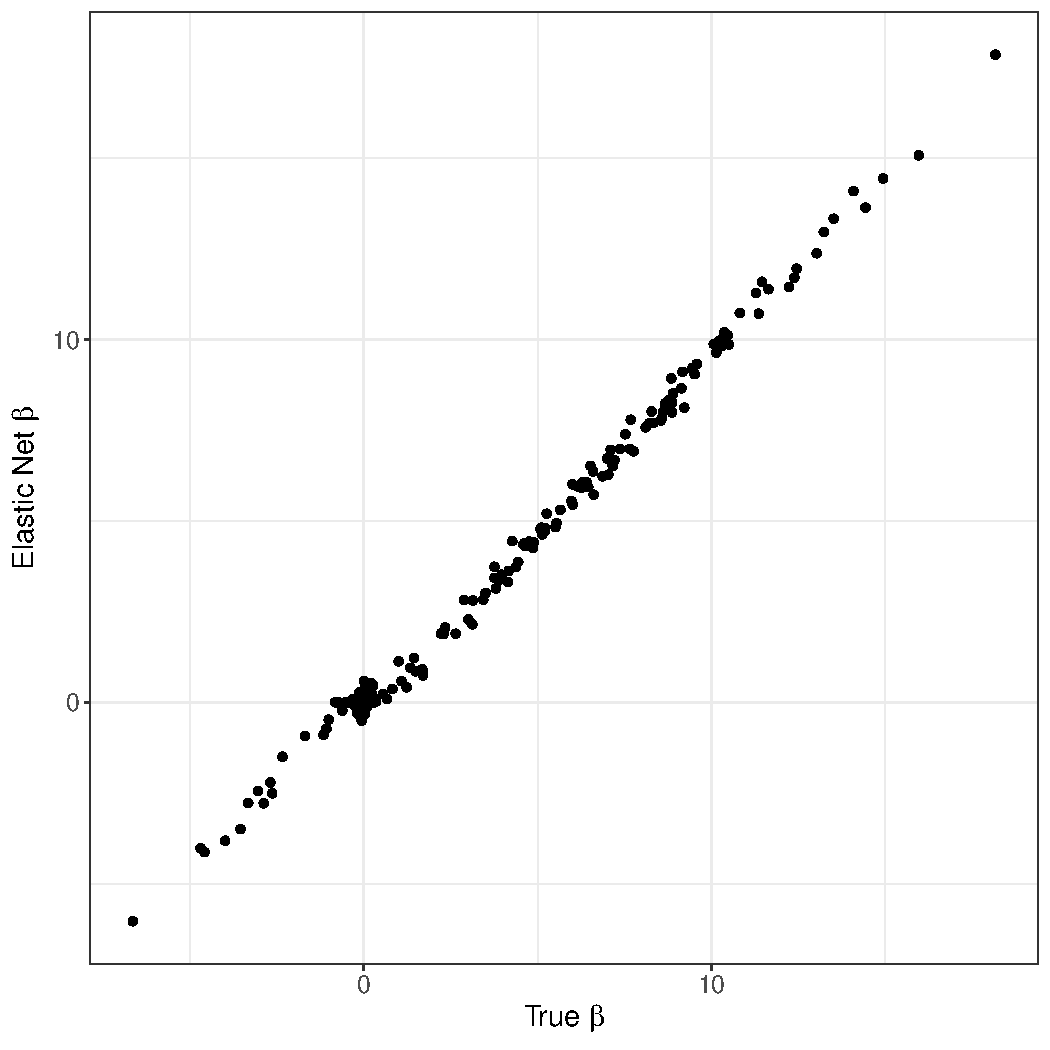
\includegraphics[width=5in]{figure/plonewbetafromenetML2-1} 

\end{knitrout}

Setting up a standard linear model with more estimators than number of observations is a fundemental assumption violation; it over-inates our coecents and gives us essentially no error. This can be really misleading to readers, and similar to how one might penalize their general linear models utilizing AIC and BIC we can use the elastic net to show more variance in our estimates and report our $\lambda$ values which are much larger than before ($\lambda$ = 10). Penalized regression is the intellectually honest thing to do when you have a model with a large number of parameters, the elastic net in this case has showed some uncertainty in our estimates whereas the normal model inflated our certainty (reported an $R^2$ of 1).


\subsection{Support Vector Models, Regression Trees}

Support Vector Models (SVMs) can be used to analize data with the least error given unsupervised machine learning. Many of these models require super computing, or a careful consideration of the data and the underlying calculus going on. Conisder the following DGP: ballanced data, split into a test set and training set. \index{DGP} \index{Test Set Training Set} \index{library() }

\begin{knitrout}
\definecolor{shadecolor}{rgb}{0.165, 0.169, 0.184}\color{fgcolor}\begin{kframe}
\begin{alltt}
\hlstd{> }\hlcom{# Need a lot of packages for this:}
\hlstd{> }\hlstd{packages} \hlkwb{<-} \hlkwd{c}\hlstd{(}\hlstr{"caret"}\hlstd{,} \hlstr{"MASS"}\hlstd{,} \hlstr{"Rlab"}\hlstd{,} \hlstr{"boot"}\hlstd{,} \hlstr{"ggplot2"}\hlstd{,} \hlstr{"ggridges"}\hlstd{,} \hlstr{"dplyr"}\hlstd{)}
\hlstd{> }\hlkwd{invisible}\hlstd{(} \hlkwd{lapply}\hlstd{(packages, library,} \hlkwc{character.only} \hlstd{=} \hlnum{TRUE}\hlstd{))}
\hlstd{> }
\hlstd{> }\hlkwd{set.seed}\hlstd{(}\hlnum{12345}\hlstd{)}
\hlstd{> }
\hlstd{> }\hlstd{N} \hlkwb{<-} \hlnum{2000}
\hlstd{> }\hlstd{P} \hlkwb{<-} \hlnum{50} \hlcom{# P is cut down for computation time, (but could be much larger!)}
\hlstd{> }
\hlstd{> }\hlcom{## Ballanced DGP creation}
\hlstd{> }\hlstd{mu} \hlkwb{<-} \hlkwd{runif}\hlstd{(P,} \hlopt{-}\hlnum{1}\hlstd{,}\hlnum{1}\hlstd{)}
\hlstd{> }\hlstd{Sigma} \hlkwb{<-} \hlkwd{rWishart}\hlstd{(}\hlkwc{n}\hlstd{=}\hlnum{1}\hlstd{,} \hlkwc{df}\hlstd{=P,} \hlkwc{Sigma}\hlstd{=}\hlkwd{diag}\hlstd{(P))[,,}\hlnum{1}\hlstd{]}
\hlstd{> }\hlstd{Sigma} \hlkwb{<-} \hlkwd{ifelse}\hlstd{(}\hlkwd{row}\hlstd{(Sigma)} \hlopt{!=} \hlkwd{col}\hlstd{(Sigma),} \hlnum{0}\hlstd{, Sigma)}
\hlstd{> }\hlstd{X} \hlkwb{<-} \hlkwd{mvrnorm}\hlstd{(N,} \hlkwc{mu}\hlstd{=mu,} \hlkwc{Sigma} \hlstd{= Sigma)}
\hlstd{> }\hlstd{p} \hlkwb{<-} \hlkwd{rbern}\hlstd{(P,} \hlnum{1}\hlstd{)}
\hlstd{> }\hlstd{beta} \hlkwb{<-} \hlstd{p}\hlopt{*}\hlkwd{rnorm}\hlstd{(P,}\hlnum{1}\hlstd{,}\hlnum{0.9}\hlstd{)} \hlopt{+} \hlstd{(}\hlnum{1}\hlopt{-}\hlstd{p)}\hlopt{*}\hlkwd{rnorm}\hlstd{(P,}\hlnum{0}\hlstd{,}\hlnum{0.3}\hlstd{)}
\hlstd{> }\hlstd{eta} \hlkwb{<-} \hlstd{X}\hlopt\hlstd{beta}
\hlstd{> }\hlstd{pi} \hlkwb{<-} \hlkwd{inv.logit}\hlstd{(eta)}
\hlstd{> }\hlstd{Y} \hlkwb{<-} \hlkwd{rbern}\hlstd{(N, pi)}
\hlstd{> }\hlstd{Y} \hlkwb{<-} \hlkwd{as.factor}\hlstd{(Y)}
\hlstd{> }\hlstd{data.1.Bal} \hlkwb{<-} \hlkwd{data.frame}\hlstd{(X, Y)}
\hlstd{> }
\hlstd{> }\hlcom{## Test/Training Sets}
\hlstd{> }\hlstd{test.data.1.Bal} \hlkwb{<-} \hlstd{data.1.Bal[}\hlnum{1}\hlopt{:}\hlnum{500}\hlstd{,]}
\hlstd{> }\hlstd{train.data.1.Bal} \hlkwb{<-} \hlstd{data.1.Bal[}\hlnum{501}\hlopt{:}\hlnum{2000}\hlstd{,]}
\end{alltt}
\end{kframe}
\end{knitrout}

With the help of a few handy packages that help users run SVM's; consider the following:

\begin{knitrout}
\definecolor{shadecolor}{rgb}{0.165, 0.169, 0.184}\color{fgcolor}\begin{kframe}
\begin{alltt}
\hlstd{> }\hlkwd{library}\hlstd{(kernlab)}
\hlstd{> }\hlkwd{library}\hlstd{(microbenchmark)}
\hlstd{> }\hlcom{# Linear SVM}
\hlstd{> }\hlstd{linear.svm.bal} \hlkwb{<-} \hlkwd{train}\hlstd{(Y}\hlopt{~}\hlstd{.,}
\hlstd{+ }                       \hlkwc{data}\hlstd{=train.data.1.Bal,}
\hlstd{+ }                       \hlkwc{method} \hlstd{=} \hlstr{"svmLinear"}\hlstd{)}
\hlstd{> }
\hlstd{> }\hlstd{linear.svm.bal}\hlopt{$}\hlstd{results}\hlopt{$}\hlstd{Accuracy}
\end{alltt}
\begin{verbatim}
## [1] 0.9651691
\end{verbatim}
\begin{alltt}
\hlstd{> }\hlcom{# A polynomial kernal: (long computation!)}
\hlstd{> }\hlcom{# poly.svm.bal <- train(Y~.,}
\hlstd{> }\hlcom{#                      data=train.data.1.Bal,}
\hlstd{> }\hlcom{#                      method="svmPoly")}
\hlstd{> }
\hlstd{> }\hlcom{# poly.svm.bal$results[as.numeric(rownames(poly.svm.bal$bestTune)),]}
\hlstd{> }\hlcom{# .951 Accuracy; .902 Kappa; AccuracySD of .011}
\hlstd{> }
\hlstd{> }
\hlstd{> }\hlcom{# Radial kernal:}
\hlstd{> }\hlcom{# radial.svm.bal = train(Y~.,}
\hlstd{> }\hlcom{#                        data=train.data.1.Bal,}
\hlstd{> }\hlcom{#                        method="svmRadialCost")}
\hlstd{> }
\hlstd{> }\hlcom{# radial.svm.bal$results[as.numeric(rownames(radial.svm.bal$bestTune)),]}
\hlstd{> }\hlcom{# Accuracy of .54; AccuracySD .017}
\end{alltt}
\end{kframe}
\end{knitrout}

Dangerously simple, this is how an SVM is ran, and could be ran given the need for a polynomial or radial kernal. The microbenchmark package is included above for any timing related concerns conduciting research with more advanced kernals.

So what's going on exactly? Well, an SVM classifies data “better” by calculating the distances between points and a line (or plane) drawn through the data. The minimal errors between these points and the plane generates more reliable classification models. This is different from a strandard regression least-squared-errors approach because this uses Euclidean distance, which is different from a vertically measured residual (commonly seen in linear models). Beyond this, we can specify various kernals to attempt to classify our data throughout various dimensions -- something the standard linear model would struggle to accomplish. Overall our data seem to classify about the same as the elastic net for ballanced data.

Another option, however, is to use classification trees for visualization and confirmation of results paired with other machine learning techniques. Below is code to accomplish this if you so choose:


\begin{knitrout}
\definecolor{shadecolor}{rgb}{0.165, 0.169, 0.184}\color{fgcolor}\begin{kframe}
\begin{alltt}
\hlstd{> }\hlcom{# Using "rpart", may need to reload R to get things to work.}
\hlstd{> }\hlkwd{library}\hlstd{(rpart)}
\hlstd{> }\hlcom{# grow tree with same DGP as above.}
\hlstd{> }\hlstd{tree.bal} \hlkwb{<-} \hlkwd{rpart}\hlstd{(Y}\hlopt{~}\hlstd{.,}
\hlstd{+ }                  \hlkwc{method} \hlstd{=} \hlstr{"class"}\hlstd{,}
\hlstd{+ }                  \hlkwc{data} \hlstd{= train.data.1.Bal)}
\hlstd{> }\hlcom{## other options include:}
\hlstd{> }\hlcom{# printcp(tree.bal) # display the results}
\hlstd{> }\hlcom{# plotcp(tree.bal)  # visualize cross-validation results}
\hlstd{> }\hlcom{# summary(tree.bal) # detailed summary of splits}
\hlstd{> }
\hlstd{> }\hlcom{# plot tree}
\hlstd{> }\hlkwd{plot}\hlstd{(tree.bal,} \hlkwc{uniform} \hlstd{=} \hlnum{TRUE}\hlstd{,}
\hlstd{+ }     \hlkwc{main} \hlstd{=} \hlstr{"Classification Tree for Ballanced Data"}\hlstd{)}
\hlstd{> }\hlkwd{text}\hlstd{(tree.bal,} \hlkwc{use.n} \hlstd{=} \hlnum{TRUE}\hlstd{,} \hlkwc{all} \hlstd{=} \hlnum{TRUE}\hlstd{,} \hlkwc{cex} \hlstd{=} \hlnum{.8}\hlstd{)}
\end{alltt}
\end{kframe}
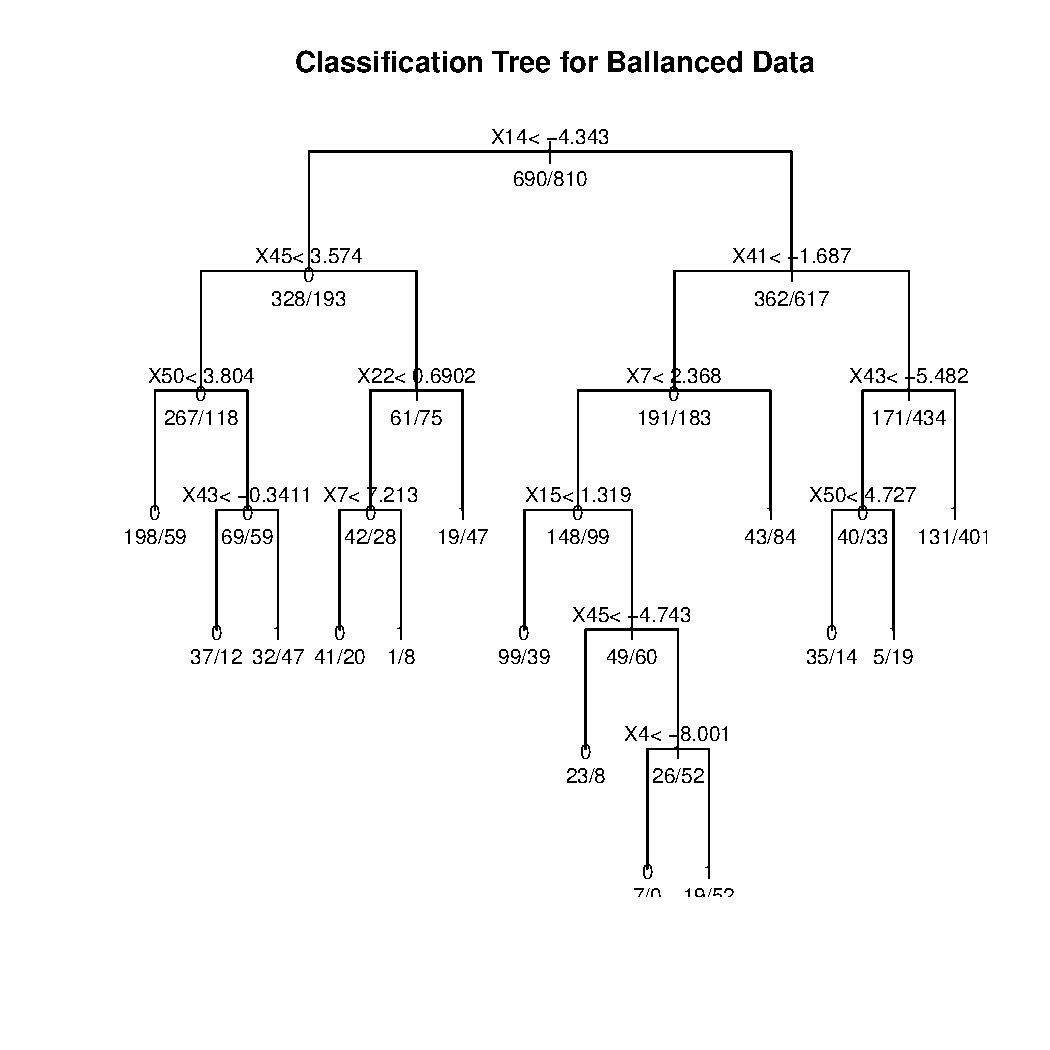
\includegraphics[width=5in]{figure/treesML1-1} 
\begin{kframe}\begin{alltt}
\hlstd{> }\hlcom{# create attractive postscript plot of tree}
\hlstd{> }\hlkwd{post}\hlstd{(tree.bal,}
\hlstd{+ }     \hlkwc{title} \hlstd{=} \hlstr{"Classification Tree for Ballanced Data"}\hlstd{)}
\hlstd{> }\hlcom{# then we have a lot of options off of this, including pruning the tree back,}
\hlstd{> }\hlcom{# or making -multiple- trees into a "forest" and}
\hlstd{> }\hlcom{# selecting the best one! (intutively a form of advanced bootstrapping!)}
\hlstd{> }\hlcom{# prune the tree, by the error that was previously generated above}
\hlstd{> }
\hlstd{> }
\hlstd{> }\hlcom{# prune function:}
\hlstd{> }\hlstd{ptree.bal} \hlkwb{<-} \hlkwd{prune}\hlstd{(tree.bal,}
\hlstd{+ }                   \hlkwc{cp}\hlstd{=tree.bal}\hlopt{$}\hlstd{cptable[}\hlkwd{which.min}\hlstd{(tree.bal}\hlopt{$}\hlstd{cptable[,}\hlstr{"xerror"}\hlstd{]),}
\hlstd{+ }                                       \hlstr{"CP"}\hlstd{])}
\hlstd{> }
\hlstd{> }\hlcom{# plot the pruned tree}
\hlstd{> }\hlkwd{plot}\hlstd{(ptree.bal,} \hlkwc{uniform} \hlstd{=} \hlnum{TRUE}\hlstd{,}
\hlstd{+ }     \hlkwc{main} \hlstd{=}\hlstr{"Pruned Classification Tree for Ballanced Data"}\hlstd{)}
\hlstd{> }\hlkwd{text}\hlstd{(ptree.bal,} \hlkwc{use.n} \hlstd{=} \hlnum{TRUE}\hlstd{,} \hlkwc{all} \hlstd{=} \hlnum{TRUE}\hlstd{,} \hlkwc{cex} \hlstd{=} \hlnum{.8}\hlstd{)}
\end{alltt}
\end{kframe}
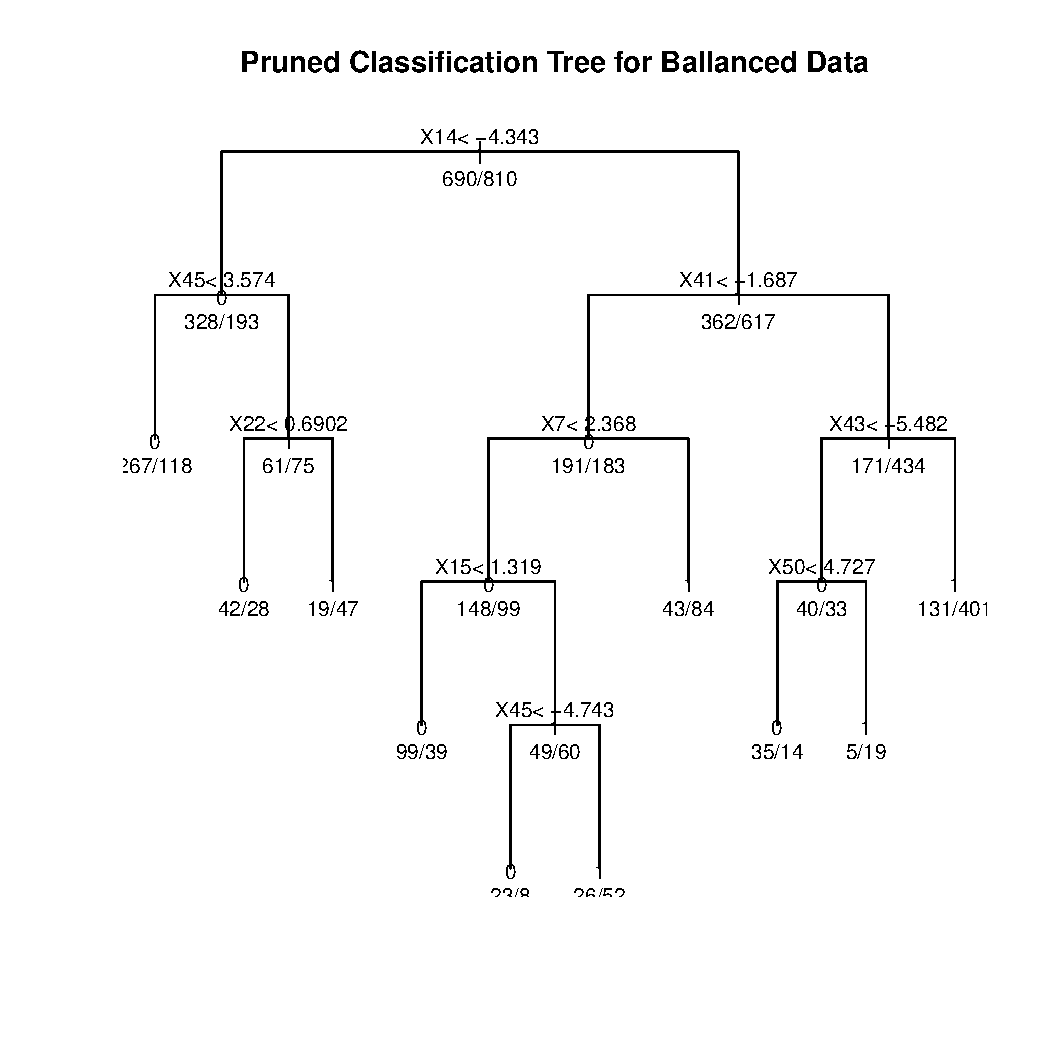
\includegraphics[width=5in]{figure/treesML1-2} 
\begin{kframe}\begin{alltt}
\hlstd{> }\hlkwd{post}\hlstd{(ptree.bal,}
\hlstd{+ }     \hlkwc{title} \hlstd{=} \hlstr{"Pruned Classification Tree for Ballanced Data"}\hlstd{)}
\end{alltt}
\end{kframe}
\end{knitrout}

Overall, regression trees (here they are classification trees) can be used to see which predictors lead our classifications, and similar to how elastic nets will bring some predictors to zero; we can then ``prune'' these observations and vizualize this process better. In poorly predictive data, this will become well pruned to only a few key observations. Reporting these over other methods may be more intuitive for readers and reviewers!

Those familiar to machine learning will note the similarity between these models to principle components analysis (PCA) -- because it is very close.



\subsection{K Nearest Neighbors, Nearest Means}




%--------------------------------------
\clearpage
\section{Timeseries}

Timeseries analysis allows us to address normative questions in a better more honest light. Timeseries operates around the difference function which will be introducted in an upcoming section. However, one benefit of timeseries is to aid humanitarian or government goals with forecasting - a worthwhile skill to develop. How parties move to an equilibrium or summarize their shocks, move together or towards a shifting eqilibrium, how they reach the equilibrium and at what rate, what structural changes effect these models, or how the very DGP itself changes are all questions best examined by timeseries.

Much of this section on timeseries comes from a course and associated text from Janet M. Box-Steffensmeir, John R. Freeman, Jon C. W. Pevehouse, and Matthew P. Hitt titled `` Time Series Analysis for the Social Sciences.'' I would highly reccomend this text if a reader is serious about learning timeseries analysis, sections of the book will be referenced in this section of the document.

\subsection{Data Concerns}

Timeseries does not rid itself of serious data concerns, and actually new data concerns arise with time series data. First, one should be aware of data vintaging: or where data is not finalized and there is some recency bias in reporting. For example, government data or live polling data may not be finalized or the process of collecting data is not complete. Older data is less controversial (usually!) but recent data can be more debateable. Robertson and Tallman have a 1998 Economic Review article discussing this in more detail. \index{Data Vintaging} \index{VAR}

Another potential concern to take seriously is systematic sampling and temporal aggregation. This is where regular interval (systematic sampling) occurs but not for the entire series. Naively a researcher may aggregate across the cross-sections but further arise if the reason why the data is missing relates to the variables in the data. For example, government data missing a few years around a particular scandal or tragety. Further, we might consider what the natural time-unit of data really is in the first place. What is the naturally occuring time of a vote, of opinions, or of healthcare? Is a vaccine or survey best distributed by the year, or by the month? This largely depends on the research question, and we may not always have the ability to best measure our natural time scale, creating noise or missing shocks where they may actually exist. \index{systematic sampling}

Finally, less of a data concern but rather a justification of the methods to follow when one might consider just adding a lagged time variable within a regression model. Doing this does not solve exogenaity problems (there's a Journal of Politics article related to this) and we will just end up with an extra function that calculates the bias from aggregation. Further, if there are multiple frequencies we could instead just measure those with a variation of the VAR (upcoming section). Adding time into a regular regression is very restrictive when we could use a VAR to pick up lag lengths or a simultanious regression model built for such variables.

\subsection{Differencing Equations and Operators}

Much like mothers all around the world demanding their children eat vegetables, methodologists too have stressed the importance of learning differencing equations for timeseries analysis. This is well covered in the Box-Steffensmeier et al. appendix - giving students a full introduction to differencing equations and trends.

Much like functions in R, or mathmatical operators, differencing equations too could be called a usages of various operators. For simplicity I will start by calling them differencing operators or a variant of the ``backshift operators.'' These are functions in the same way that $f(x)$ is a function being applied to $x$. Instead, with the differencing operators ($\Delta$) we mean, simply, $(1-B)$ where B is just a lag operator (or the backshift operator). The ``difference'' synonym comes from the subtraction of $1-B$.

For clarity, these two are equivilent:

\begin{equation}
\Delta (.5^t) = .5^t - .5^{t-1}
\end{equation}

And the backshift operator acts simply:
\begin{equation}
B(.5^t) = .5^{t-1}
\end{equation}

And the square of this function works similarly:

\begin{equation}
\Delta^2 y(t) = (1-B)^2 y(t) = (1-2B + B^2) y(t) = y(t) - 2y(t-1) + y(t-2).
\end{equation}

Or with $.5^t$ as $y(t)$ we have:

\begin{equation}
\Delta^2(.5^t) = .5^t - 2(.5^{t-1}) +.5^{t-2} = .5^t
\end{equation}

Finally, we have a third operator to help us and that is the ``expectations'' or ``lead'' operator (E). Which brings our variable forward a time period.

\begin{equation}
Ey(t) = y(t+1)
\end{equation}

Difference equations, then, are the intregate combination of these operators to produce particular equalities. Standard regression models often do not consider these nuances, but the study of difference equations helps us understand the dynamics that are implicit in our time series related equations.


\subsection{Identifying AR;MA - ACF, PACF}


\subsection{Unit Roots}


\subsection{ARIMA}


\subsection{VAR}

\subsubsection{Example VAR}

\begin{knitrout}
\definecolor{shadecolor}{rgb}{0.165, 0.169, 0.184}\color{fgcolor}\begin{kframe}
\begin{alltt}
\hlstd{> }\hlcom{# devtools::install_github("hadley/haven")}
\hlstd{> }\hlkwd{require}\hlstd{(haven)}
\hlstd{> }\hlstd{df} \hlkwb{<-} \hlkwd{read_dta}\hlstd{(}\hlstr{'C:/Users/Shing/Documents/GodGap/TS Final/anes_timeseries_cdf.dta'}\hlstd{)}
\hlstd{> }\hlkwd{library}\hlstd{(ggplot2)}
\hlstd{> }\hlkwd{library}\hlstd{(ggthemes)}
\end{alltt}
\end{kframe}
\end{knitrout}

\begin{center}
\begin{knitrout}
\definecolor{shadecolor}{rgb}{0.165, 0.169, 0.184}\color{fgcolor}
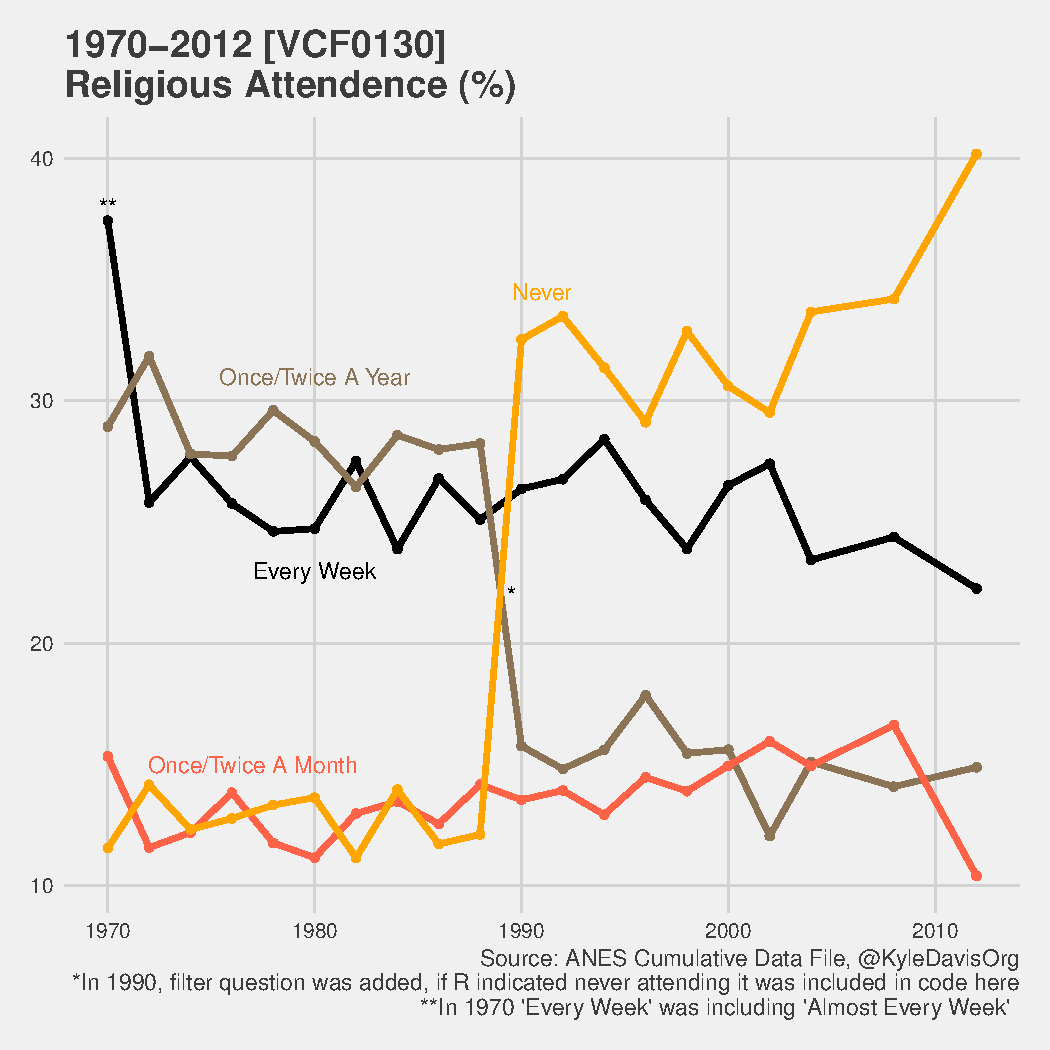
\includegraphics[width=6in,height=3.7in]{figure/desc-1} 

\end{knitrout}
\end{center}

Using the ANES data, we see some survey changes over time on how we measured religious attendence. To narrow down, I will be analyizing only those respondents that reported weekly attendence. Further, I will be looking at those who reported being ``strongly liberal'' (conservative) including leaning liberal (conservative). Since the latter question was only asked from 1972 on, I will subset the weekly church attendence from 1972 to 2012. This has an unexpected benefit of removing the 1970 survey change on weekly church attendence.

\begin{center}
\begin{knitrout}
\definecolor{shadecolor}{rgb}{0.165, 0.169, 0.184}\color{fgcolor}
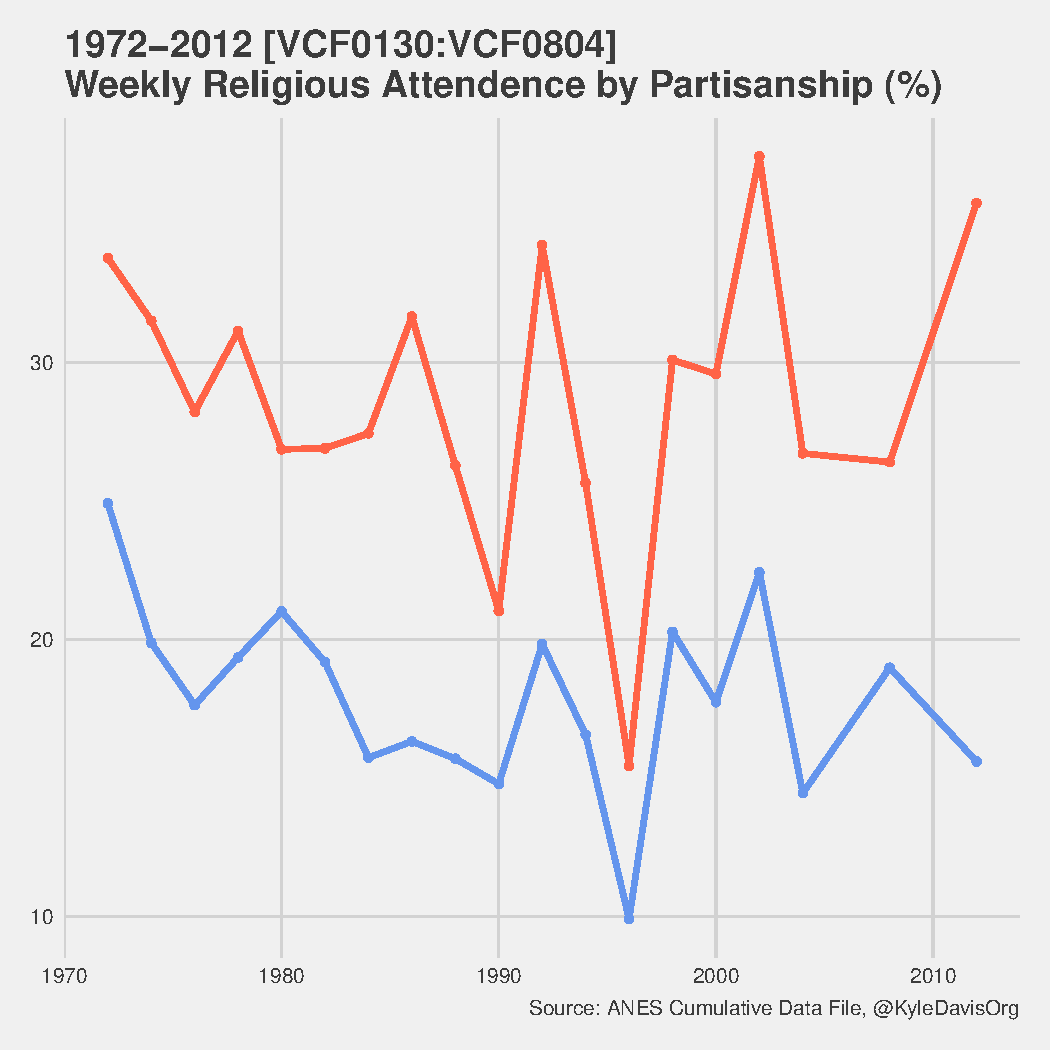
\includegraphics[width=6in,height=4in]{figure/descriptiveplot-1} 

\end{knitrout}
\end{center}

Using this data, I wish to formally test that the two series are not granger-causal of one another and that the two trends are not deterministic of the other. It is my hypothesis that the two series do not rely on one another, but larger economic and sociopolitical influences are at play. Following testing this hypothesis, I will end this assignment discussing future directions.

\textbf{Testing for Optimal Lag Order for VAR}

Before I begin testing for optimal lag length for the model, I test for the presence of unit roots. The following chunk of R code goes through setting up the data and conducting unit root tests. It reveals that in every unit root test I conduct, there is evidence against the presence of unit roots and nonstationarity.\footnote{In setting up the time series in R, I had to set the end date back, to get the right frequency to line up with skipped year surveys. Regardless, all data is still present, the year index label for 2012 is, however, masked. This should not change any results, I checked the plots between the full ANES dat and the time series object reported here for any discrepencies, finding none.}

\begin{knitrout}
\definecolor{shadecolor}{rgb}{0.165, 0.169, 0.184}\color{fgcolor}\begin{kframe}
\begin{alltt}
\hlstd{> }\hlstd{libweekTS} \hlkwb{<-} \hlkwd{ts}\hlstd{(}\hlkwc{data} \hlstd{= libweek[,}\hlnum{2}\hlstd{],}
\hlstd{+ }                \hlkwc{start} \hlstd{=} \hlkwd{head}\hlstd{(year,} \hlkwc{n} \hlstd{=} \hlnum{1}\hlstd{),}
\hlstd{+ }                \hlkwc{end} \hlstd{=} \hlnum{2008}\hlstd{,} \hlcom{# 2008 end here because ANES aregular surveys}
\hlstd{+ }                \hlkwc{frequency} \hlstd{=} \hlnum{.5}\hlstd{)}
\hlstd{> }\hlcom{# plot(libweekTS) # Checking}
\hlstd{> }
\hlstd{> }\hlstd{consweekTS} \hlkwb{<-} \hlkwd{ts}\hlstd{(}\hlkwc{data} \hlstd{= consweek[,}\hlnum{2}\hlstd{],}
\hlstd{+ }                \hlkwc{start} \hlstd{=} \hlkwd{head}\hlstd{(year,} \hlkwc{n} \hlstd{=} \hlnum{1}\hlstd{),}
\hlstd{+ }                \hlkwc{end} \hlstd{=} \hlnum{2008}\hlstd{,}
\hlstd{+ }                \hlkwc{frequency} \hlstd{=} \hlnum{.5}\hlstd{)}
\hlstd{> }\hlcom{# plot(consweekTS) # Checking}
\hlstd{> }
\hlstd{> }\hlcom{## Unit root testing:}
\hlstd{> }\hlkwd{library}\hlstd{(tseries)}
\hlstd{> } \hlkwd{adf.test}\hlstd{(libweekTS)}
\hlstd{> } \hlkwd{adf.test}\hlstd{(consweekTS)}
\hlstd{> }\hlcom{# Reject the null of non - stationarity and a unit root}
\hlstd{> }
\hlstd{> } \hlkwd{kpss.test}\hlstd{(libweekTS)}
\hlstd{> } \hlkwd{kpss.test}\hlstd{(consweekTS)}
\hlstd{> }\hlcom{# Reject the null of stationarity around a deterministic trend}
\hlstd{> }
\hlstd{> } \hlkwd{PP.test}\hlstd{(libweekTS)}
\hlstd{> } \hlkwd{PP.test}\hlstd{(consweekTS)}
\hlstd{> }\hlcom{# Reject the null that the series is integrated of order 1 (unit root)}
\end{alltt}
\end{kframe}
\end{knitrout}

Following these tests I feel confident that there are no unit roots. Moving to testing the lag-order of the model is realitively easy to do in R, and give us the lag order based upon different information critera such as the AIC, HQ, SC, and FPE. Results of these tests all indicate best lag-length of four. \index{Augmented Dicky Fuller} \index{KPSS Test}

\begin{knitrout}
\definecolor{shadecolor}{rgb}{0.165, 0.169, 0.184}\color{fgcolor}\begin{kframe}
\begin{alltt}
\hlstd{> }\hlcom{# Ideal lag order:}
\hlstd{> }\hlstd{varData} \hlkwb{<-} \hlkwd{data.frame}\hlstd{(libweekTS, consweekTS)}
\hlstd{> }
\hlstd{> }\hlkwd{library}\hlstd{(vars)}
\hlstd{> }
\hlstd{> }\hlstd{lagselection} \hlkwb{<-} \hlkwd{VARselect}\hlstd{(varData,} \hlkwc{lag.max} \hlstd{=} \hlnum{10}\hlstd{,} \hlkwc{type} \hlstd{=} \hlstr{"none"}\hlstd{)}
\hlstd{> }\hlstd{lagselection}\hlopt{$}\hlstd{selection}
\end{alltt}
\begin{verbatim}
## AIC(n)  HQ(n)  SC(n) FPE(n) 
##      4      4      4      4
\end{verbatim}
\end{kframe}
\end{knitrout}

\textbf{Granger--Causality Test} \index{Granger Causality}

A time series is said to be Granger-causal to an outcome if it (through lagged values) can provide statistically significant information about the outcome. This relationship is based upon two requirements: the cause happens prior to its effect (lagged values), and the cause provides unique information about the future values of its effect. These assumptions are in some-way built into nearly every cause inference test. \index{Vector Auto Regression}

More specifically, a variable $X$ is Granger-causal to some $Y$ if the prediction of $Y_t$ based upon all of its past lagged values $(Y_{t-1}, Y_{t-2}, ...)$ and on lagged values of $X$ does better than just $Y$ based solely on it's past values alone. Put another way, granger-causality compares two predictive models (``worlds''), one where $X$ exists or where $Y$ is soley predictive upon itself. If the model which includes $X$ does better than the $Y$ being predictive of itself, $X$ is said to be Granger-causal of $Y$.

\begin{knitrout}
\definecolor{shadecolor}{rgb}{0.165, 0.169, 0.184}\color{fgcolor}\begin{kframe}
\begin{alltt}
\hlstd{> }\hlstd{var1} \hlkwb{<-} \hlkwd{VAR}\hlstd{(varData,} \hlkwc{p}\hlstd{=}\hlnum{4}\hlstd{,} \hlkwc{type}\hlstd{=}\hlstr{"const"}\hlstd{)} \hlcom{# Indicating lag length 4 here.}
\hlstd{> } \hlcom{# summary(var1) VAR results, including a 4-lag model results.}
\hlstd{> } \hlcom{# plot(var1) # can easily check ACF and PACF here}
\hlstd{> }
\hlstd{> } \hlstd{granger1} \hlkwb{<-} \hlkwd{causality}\hlstd{(var1,} \hlkwc{cause}\hlstd{=}\hlstr{"consweekTS"}\hlstd{)}
\hlstd{> } \hlstd{granger1}\hlopt{$}\hlstd{Granger}\hlopt{$}\hlstd{method}
\end{alltt}
\begin{verbatim}
## [1] "Granger causality H0: consweekTS do not Granger-cause libweekTS"
\end{verbatim}
\begin{alltt}
\hlstd{> } \hlstd{granger1}\hlopt{$}\hlstd{Granger}\hlopt{$}\hlstd{p.value}
\end{alltt}
\begin{verbatim}
##           [,1]
## [1,] 0.3452188
\end{verbatim}
\begin{alltt}
\hlstd{> } \hlstd{granger2} \hlkwb{<-} \hlkwd{causality}\hlstd{(var1,} \hlkwc{cause}\hlstd{=}\hlstr{"libweekTS"}\hlstd{)}
\hlstd{> } \hlstd{granger2}\hlopt{$}\hlstd{Granger}\hlopt{$}\hlstd{method}
\end{alltt}
\begin{verbatim}
## [1] "Granger causality H0: libweekTS do not Granger-cause consweekTS"
\end{verbatim}
\begin{alltt}
\hlstd{> } \hlstd{granger2}\hlopt{$}\hlstd{Granger}\hlopt{$}\hlstd{p.value}
\end{alltt}
\begin{verbatim}
##           [,1]
## [1,] 0.9601701
\end{verbatim}
\end{kframe}
\end{knitrout}


This hypothesis test takes as the null that $X$ is not a Granger-cause of $Y$ , and as such, a p-value below some $\alpha$ level would lead one to reject the null hypothesis. These tests lead me to confirm that neither series is Granger-causal of the other. Placed back in theory, neither liberals nor conservatives follow each others trends in weekly church attendence -- indicating other sociological, political, or economic forces to be at play.

A sign-and-significance reading of the Granger causality results conclude that, with 12 degrees of freedom, neither variation of the Granger-causaility test pass statistical significance to declare Granger-causality. The liberal timeseries onto the conservative series holds a p-value of .96, and the conservative series on the liberal holds a p-value of .34. Neither pass conventional .05 thresholds because the series better explains itself than other explains it with respect to the VAR with lag length four.


\textbf{Innovation Accounting} \index{Innovation Accounting}


Innovation accounting can tell us how a VAR model responds to individual and orthogonalized shocks to each of the variables. This necceciates an assumption that our variable orderings matter as these shocks transition through our structure. However, orthogonalizing the equation allows for us to see the marginal effects, if we didn't do this we would allow the variable to increase its ripples throught the structure without controlling for confounds that could occur.

In this particular case I am not sure if the ordering of variables really matters much, I think respondents from  year-to-year don't really consider their parties past responses to church identification all that much. The figure below kind-of shows this, a moving around 0, insignificant on starndard thresholds.

Finally we move to looking at the forecast error variance decomposition, which allows for examining the effect of a particular variable to the future forecast error variance of another variable. To examine this, see the plots below the innovation accounting. These reveal that not one particular variable is contributing to forecast uncertainty. It is notable, however, that the FEVD did detect some variance explained by liberal church attendence on liberal church attendence in the first two horizons.


\begin{center}
\begin{knitrout}
\definecolor{shadecolor}{rgb}{0.165, 0.169, 0.184}\color{fgcolor}\begin{kframe}
\begin{alltt}
\hlstd{> }\hlcom{# Innovation accounting:}
\hlstd{> } \hlstd{irf1} \hlkwb{<-} \hlkwd{irf}\hlstd{(var1,} \hlkwc{impulse} \hlstd{=} \hlstr{"consweekTS"}\hlstd{,} \hlkwc{response} \hlstd{=} \hlstr{"libweekTS"}\hlstd{)}
\hlstd{> } \hlkwd{plot}\hlstd{(irf1)}
\end{alltt}
\end{kframe}
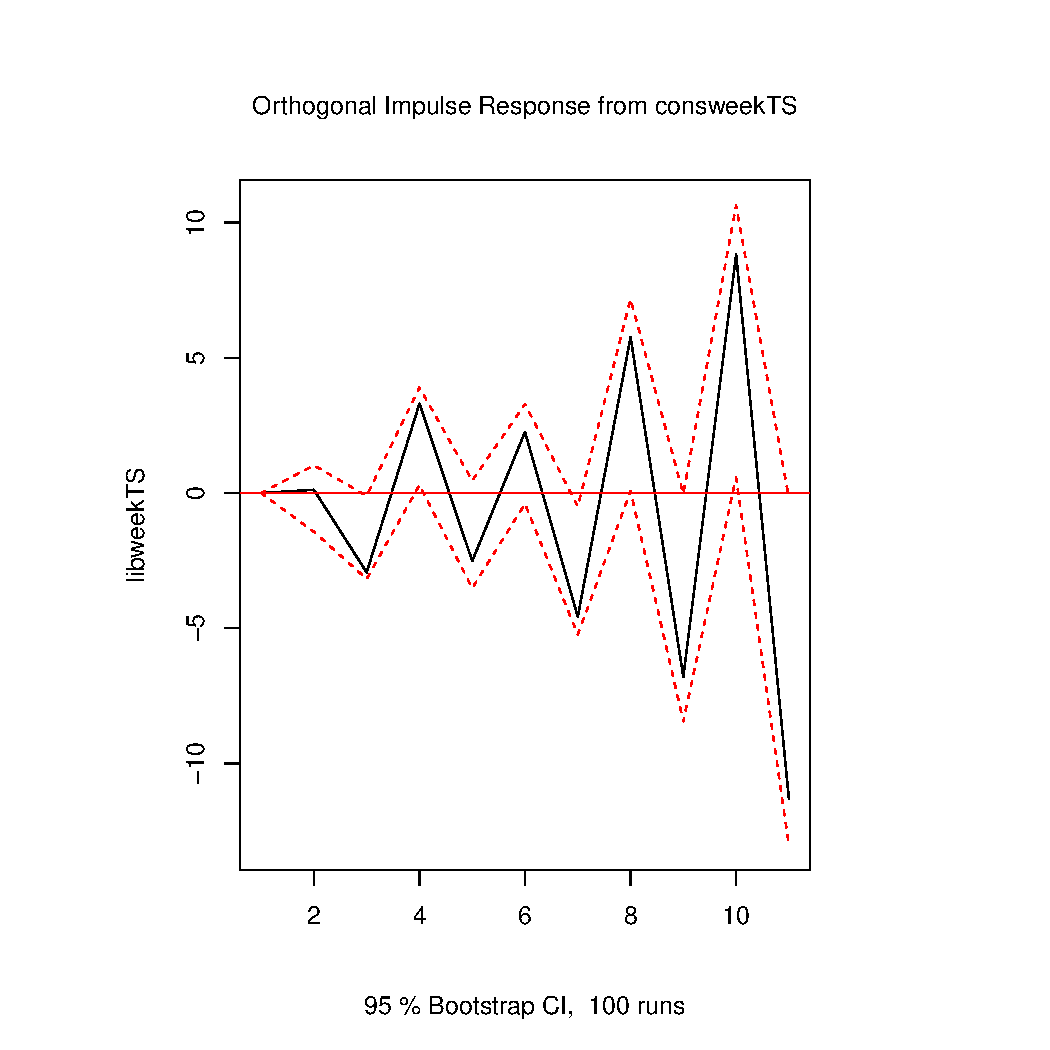
\includegraphics[width=\maxwidth,height=4.5in]{figure/inov-1} 
\begin{kframe}\begin{alltt}
\hlstd{> } \hlstd{irf2} \hlkwb{<-} \hlkwd{irf}\hlstd{(var1,} \hlkwc{impulse} \hlstd{=} \hlstr{"libweekTS"}\hlstd{,} \hlkwc{response} \hlstd{=} \hlstr{"consweekTS"}\hlstd{)}
\hlstd{> } \hlkwd{plot}\hlstd{(irf2)}
\end{alltt}
\end{kframe}
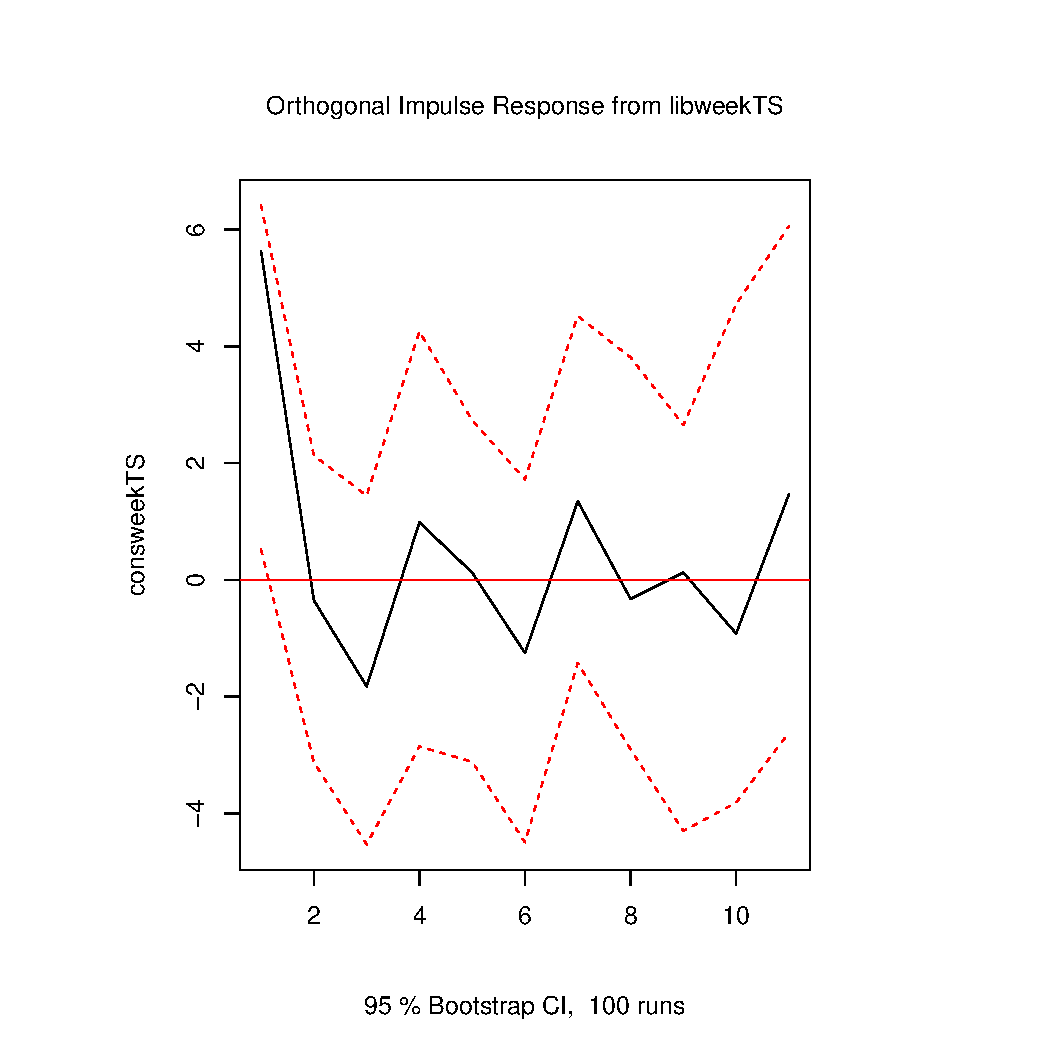
\includegraphics[width=\maxwidth,height=4.5in]{figure/inov-2} 
\begin{kframe}\begin{alltt}
\hlstd{> }\hlcom{# Forecast Error Variance Decomposition}
\hlstd{> } \hlstd{fevd1} \hlkwb{<-} \hlkwd{fevd}\hlstd{(var1,} \hlkwc{n.ahead} \hlstd{=} \hlnum{5}\hlstd{)}
\hlstd{> } \hlkwd{plot}\hlstd{(fevd1)}
\end{alltt}
\end{kframe}
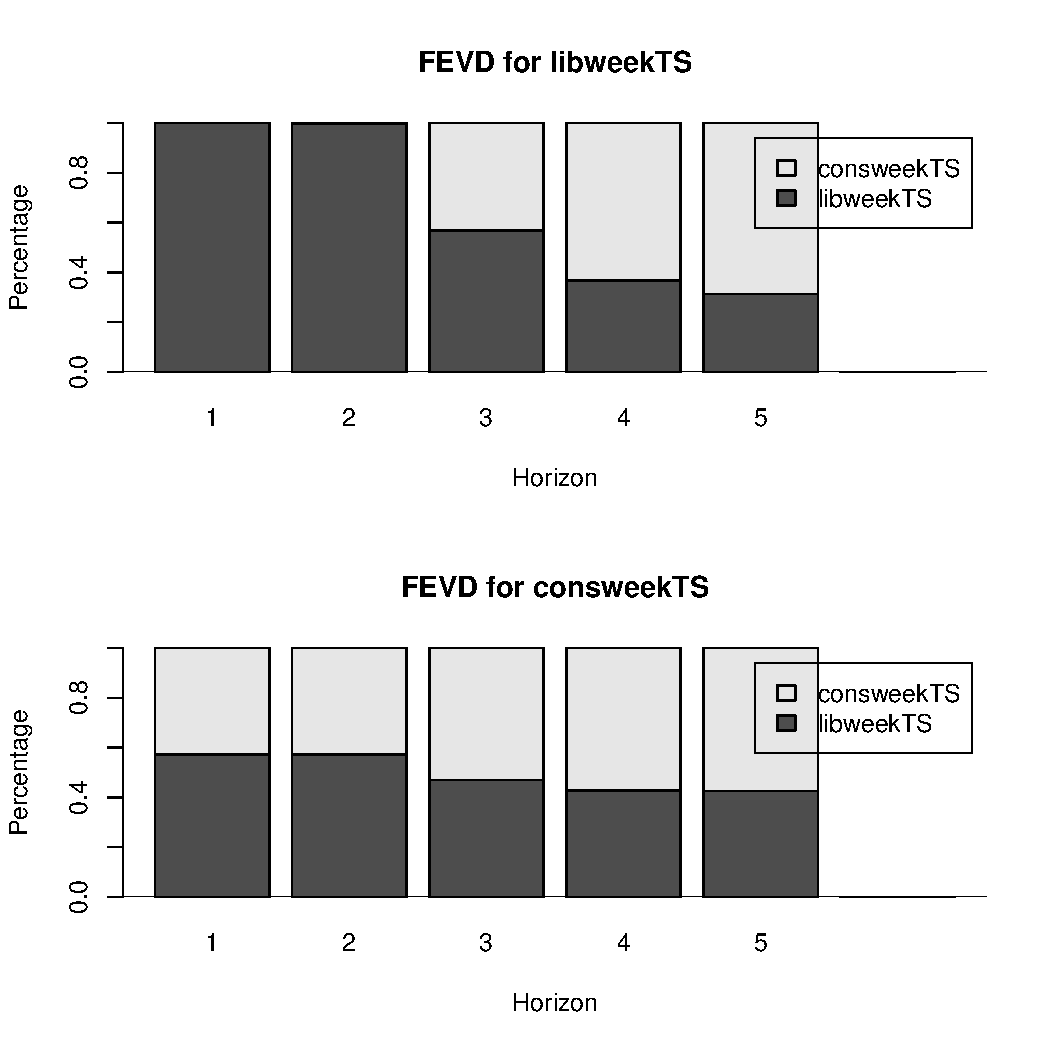
\includegraphics[width=\maxwidth,height=4.5in]{figure/inov-3} 

\end{knitrout}
\end{center}


\textbf{Summary, Concluding Thoughts}

Overall, the purpose of this assignment was to test the relationship between two series and report how they may relate or not. I chose to test a fundemental underlying assumption of the ``god gap'' literature, for if these two series did influence one-another then all past examinations would need to take in to account this. However I have found little evidence of this occuring. This makes sense, survey responses of one partisan on church attendence are likely not to consider the other partisan and their historical activites. Rather, I think larger socioeconomic, historical, and geographical variables matter more at moving partisians to church at different levels over time. VAR too can be used to study these variables in realtion to the others.

While VAR allows for flexibility in helping determine the data generating process, proper treatment of the error term through lag-length detection, and easy transition to error correction models and OLS it is not without its disadvantages. If a series is nonstationary, statistical testing can become problematic.\footnote{Box-Steffensmeier, Janet M., John R. Freeman, Matthew P. Hitt, and Jon CW Pevehouse. Time series analysis for the social sciences. \textit{Cambridge University Press}, 2014.} If the series is cointegrated differencing may not solve these problems. Finally, as I mentioned before, I think a lot of different variables influence the widening and contraction of the god gap, however including all of them for all of their past lags may easily overfit the model if proper percautions are not used.\footnote{Many thanks to Benjamin Campbell for his help with the coding and theory behind these methods.}



%--------------------------------------
\clearpage
\section{Network Analysis}

\subsection{Network Theory}

\subsection{Network Data, Nodes, and Edges}

\subsection{Summary Statistics of Networks}

\subsection{Centrality}

Measuring the centrality of a network is indicating which node(s) are most central, or critical, to the network remaning the shape it is in. A central node, for example, can be the person inbetween groups, or just a well connected node in general. There are many ways to measure and detect network centrality, some of which I've studied are listed below. Later in this section we will compare each of these finding that they typically correlate with one another (good!). Cannon advice is to report all of the relevant measures of centrality rather than spending too much time choosing any particular one.

\textit{Borgatti (2005):}
\begin{longtable}{m{2.8cm}  m{4cm} m{5.7cm} m{4.7cm}  }
\hline\noalign{\smallskip}
\textbf{Name} & \textbf{Definition} & \textbf{Properties} & \textbf{Notes} \\
\noalign{\smallskip}\hline\noalign{\smallskip}
Betweenness (Freeman, 1979) & $\mathlarger{ \Sigma_i \Sigma_j \frac{g_{ikj}}{g_{ij}}, ~~ i \neq j \neq k }$ & Assumes traffic is indivisible, traffic takes known-shortest paths,   & Likely not a good index for information flow or ``gossip'' \\
Eigenvector centrality (Bonacich, 1972) & $\lambda v = A v$ & Traffic moves along unrestricted ``walks.'' Traffic can effect subsequent nodes simultaneously. Measures long term and indirect risk.   & Related to other measures on sequentially influencing nodes (``influence-type process'').\\
Degree centrality (Freeman, 1979) & Limiting probabilities of nodes by their degree. (Markov Process).    & Measures immediate risk. Assumes an infinitely long random walk (a dollar traveling hands). \\
\noalign{\smallskip}\hline\noalign{\smallskip}
\end{longtable}


But how do we actually do this? Let's start with reading in the data, and setting everything up. I'll save space by not commenting this inital code, just know that it is creating an edgelist matrix for us to generate network objects. This data is from Google's BigQuery - Reddit data in October and November (2017) for the r/asksocialscientists page. This contains those who post and those who comment. \index{recoding data}
\begin{knitrout}
\definecolor{shadecolor}{rgb}{0.165, 0.169, 0.184}\color{fgcolor}\begin{kframe}
\begin{alltt}
\hlstd{> }\hlcom{# Initial Packages:}
\hlstd{> }\hlkwd{library}\hlstd{(statnet)}
\hlstd{> }\hlkwd{library}\hlstd{(dplyr)}
\hlstd{> }\hlkwd{library}\hlstd{(igraph)}
\hlstd{> }
\hlstd{> }\hlcom{# Let's read in, add on top of one/ another the Reddit EdgeList data:}
\hlstd{> }\hlcom{##   October:}
\hlstd{> }\hlcom{# read in the posts data}
\hlstd{> }\hlstd{posts} \hlkwb{<-} \hlkwd{read.csv}\hlstd{(}\hlstr{'file:///C:/Users/Shing/Documents/Previous Course Info/Networks/Data/2017_10_AskSocialScience_posts.csv'}\hlstd{)}
\hlstd{> }\hlcom{# read in the comments data}
\hlstd{> }\hlstd{comments} \hlkwb{<-} \hlkwd{read.csv}\hlstd{(}\hlstr{'file:///C:/Users/Shing/Documents/Previous Course Info/Networks/Data/2017_10_AskSocialScience_comments.csv'}\hlstd{)}
\hlstd{> }\hlstd{comments}\hlopt{$}\hlstd{id2} \hlkwb{<-} \hlkwd{paste}\hlstd{(}\hlstr{"t1_"}\hlstd{, comments}\hlopt{$}\hlstd{id,} \hlkwc{sep}\hlstd{=}\hlstr{""}\hlstd{)}
\hlstd{> }\hlstd{posts}\hlopt{$}\hlstd{id2} \hlkwb{<-} \hlkwd{paste}\hlstd{(}\hlstr{"t3_"}\hlstd{, posts}\hlopt{$}\hlstd{id,} \hlkwc{sep}\hlstd{=}\hlstr{""}\hlstd{)}
\hlstd{> }\hlstd{for_el} \hlkwb{<-} \hlkwd{data.frame}\hlstd{(}
\hlstd{+ }     \hlkwc{author} \hlstd{=} \hlkwd{c}\hlstd{(}\hlkwd{as.character}\hlstd{(posts}\hlopt{$}\hlstd{author),} \hlkwd{as.character}\hlstd{(comments}\hlopt{$}\hlstd{author)),}
\hlstd{+ }     \hlkwc{id} \hlstd{=} \hlkwd{c}\hlstd{(}\hlkwd{as.character}\hlstd{(posts}\hlopt{$}\hlstd{id2),} \hlkwd{as.character}\hlstd{(comments}\hlopt{$}\hlstd{id2)),}
\hlstd{+ }     \hlkwc{parent_id} \hlstd{=} \hlkwd{c}\hlstd{(}\hlkwd{rep}\hlstd{(}\hlnum{NA}\hlstd{,} \hlkwd{dim}\hlstd{(posts)[}\hlnum{1}\hlstd{]),} \hlkwd{as.character}\hlstd{(comments}\hlopt{$}\hlstd{parent_id))}
\hlstd{+ }\hlstd{)}
\hlstd{> }
\hlstd{> }\hlstd{for_el} \hlkwb{<-} \hlstd{for_el[for_el}\hlopt{$}\hlstd{author}\hlopt{!=}\hlstr{"[deleted]"}\hlstd{,]}
\hlstd{> }\hlstd{el1} \hlkwb{<-} \hlkwd{inner_join}\hlstd{(for_el, for_el,} \hlkwd{c}\hlstd{(}\hlstr{"parent_id"} \hlstd{=} \hlstr{"id"}\hlstd{))}
\hlstd{> }\hlstd{el} \hlkwb{<-} \hlkwd{data.frame}\hlstd{(}\hlkwc{auth1} \hlstd{= el1}\hlopt{$}\hlstd{author.x,} \hlkwc{auth2} \hlstd{= el1}\hlopt{$}\hlstd{author.y)}
\hlstd{> }\hlstd{el} \hlkwb{<-} \hlkwd{as.matrix}\hlstd{(el)}
\hlstd{> }
\hlstd{> }\hlcom{#---------------------------------------------------------------------------}
\hlstd{> }\hlcom{##   Nov:}
\hlstd{> }\hlstd{posts2} \hlkwb{<-} \hlkwd{read.csv}\hlstd{(}\hlstr{'file:///C:/Users/Shing/Documents/Previous Course Info/Networks/Data/2017_11_AskSocialScience_posts.csv'}\hlstd{)}
\hlstd{> }\hlstd{comments2} \hlkwb{<-} \hlkwd{read.csv}\hlstd{(}\hlstr{'file:///C:/Users/Shing/Documents/Previous Course Info/Networks/Data/2017_11_AskSocialScience_comments.csv'}\hlstd{)}
\hlstd{> }\hlstd{comments2}\hlopt{$}\hlstd{id2} \hlkwb{<-} \hlkwd{paste}\hlstd{(}\hlstr{"t1_"}\hlstd{, comments2}\hlopt{$}\hlstd{id,} \hlkwc{sep}\hlstd{=}\hlstr{""}\hlstd{)}
\hlstd{> }\hlstd{posts2}\hlopt{$}\hlstd{id2} \hlkwb{<-} \hlkwd{paste}\hlstd{(}\hlstr{"t3_"}\hlstd{, posts2}\hlopt{$}\hlstd{id,} \hlkwc{sep}\hlstd{=}\hlstr{""}\hlstd{)}
\hlstd{> }
\hlstd{> }\hlstd{for_el2} \hlkwb{<-} \hlkwd{data.frame}\hlstd{(}
\hlstd{+ }     \hlkwc{author} \hlstd{=} \hlkwd{c}\hlstd{(}\hlkwd{as.character}\hlstd{(posts2}\hlopt{$}\hlstd{author),} \hlkwd{as.character}\hlstd{(comments2}\hlopt{$}\hlstd{author)),}
\hlstd{+ }     \hlkwc{id} \hlstd{=} \hlkwd{c}\hlstd{(}\hlkwd{as.character}\hlstd{(posts2}\hlopt{$}\hlstd{id2),} \hlkwd{as.character}\hlstd{(comments2}\hlopt{$}\hlstd{id2)),}
\hlstd{+ }     \hlkwc{parent_id} \hlstd{=} \hlkwd{c}\hlstd{(}\hlkwd{rep}\hlstd{(}\hlnum{NA}\hlstd{,} \hlkwd{dim}\hlstd{(posts2)[}\hlnum{1}\hlstd{]),} \hlkwd{as.character}\hlstd{(comments2}\hlopt{$}\hlstd{parent_id))}
\hlstd{+ }\hlstd{)}
\hlstd{> }\hlstd{for_el2} \hlkwb{<-} \hlstd{for_el2[for_el2}\hlopt{$}\hlstd{author}\hlopt{!=}\hlstr{"[deleted]"}\hlstd{,]}
\hlstd{> }\hlstd{el12} \hlkwb{<-} \hlkwd{inner_join}\hlstd{(for_el2, for_el2,} \hlkwd{c}\hlstd{(}\hlstr{"parent_id"} \hlstd{=} \hlstr{"id"}\hlstd{))}
\hlstd{> }\hlstd{el2} \hlkwb{<-} \hlkwd{data.frame}\hlstd{(}\hlkwc{auth1} \hlstd{= el12}\hlopt{$}\hlstd{author.x,} \hlkwc{auth2} \hlstd{= el12}\hlopt{$}\hlstd{author.y)}
\hlstd{> }\hlstd{el2} \hlkwb{<-} \hlkwd{as.matrix}\hlstd{(el2)}
\end{alltt}
\end{kframe}
\end{knitrout}

Now that we have the data read in and cleaned (mostly tracking the id numbers), I'll combine the two months and plot the network object that we'll be using for the rest of this section.

\begin{center}
\begin{knitrout}
\definecolor{shadecolor}{rgb}{0.165, 0.169, 0.184}\color{fgcolor}\begin{kframe}
\begin{alltt}
\hlstd{> }\hlcom{# Stack one edge list on top of the other:}
\hlstd{> }\hlstd{edge.list} \hlkwb{<-} \hlkwd{rbind}\hlstd{(el, el2)}
\hlstd{> }\hlkwd{head}\hlstd{(edge.list)}
\end{alltt}
\begin{verbatim}
##      auth1                 auth2          
## [1,] "ProbablyaNerd"       "AutoModerator"
## [2,] "panick21"            "dandelusional"
## [3,] "wellmanicuredman"    "abbamouse"    
## [4,] "timeimmemorial"      "dewarr"       
## [5,] "yodatsracist"        "dewarr"       
## [6,] "North_London_Gunner" "obamanisha"
\end{verbatim}
\begin{alltt}
\hlstd{> }\hlstd{graph.object} \hlkwb{<-} \hlkwd{graph_from_edgelist}\hlstd{(edge.list)}
\hlstd{> }\hlkwd{summary}\hlstd{(graph.object)} \hlcom{# Basic statistics seem okay}
\end{alltt}
\begin{verbatim}
## IGRAPH 26bd3b7 DN-- 610 1043 -- 
## + attr: name (v/c)
\end{verbatim}
\begin{alltt}
\hlstd{> }\hlcom{# Grabbing the largest component:}
\hlstd{> }\hlstd{giant.component} \hlkwb{<-} \hlkwa{function}\hlstd{(}\hlkwc{graph}\hlstd{) \{}
\hlstd{+ }     \hlstd{cl} \hlkwb{<-} \hlkwd{clusters}\hlstd{(graph)}
\hlstd{+ }     \hlkwd{induced.subgraph}\hlstd{(graph,} \hlkwd{which}\hlstd{(cl}\hlopt{$}\hlstd{membership} \hlopt{==} \hlkwd{which.max}\hlstd{(cl}\hlopt{$}\hlstd{csize)))}
\hlstd{+ }\hlstd{\}}
\hlstd{> }
\hlstd{> }\hlstd{l.graph.object} \hlkwb{<-} \hlkwd{giant.component}\hlstd{(graph.object)}
\hlstd{> }
\hlstd{> }\hlcom{# Let's graph it}
\hlstd{> }\hlkwd{par}\hlstd{(}\hlkwc{mfrow}\hlstd{=}\hlkwd{c}\hlstd{(}\hlnum{1}\hlstd{,}\hlnum{2}\hlstd{))}
\hlstd{> }\hlkwd{plot.igraph}\hlstd{(graph.object,}
\hlstd{+ }            \hlkwc{vertex.color}\hlstd{=}\hlstr{"gray15"}\hlstd{,}
\hlstd{+ }            \hlkwc{vertex.size}\hlstd{=}\hlnum{2.7}\hlstd{,}
\hlstd{+ }            \hlkwc{vertex.label}\hlstd{=}\hlnum{NA}\hlstd{,}
\hlstd{+ }            \hlkwc{vertex.shape}\hlstd{=}\hlstr{"circle"}\hlstd{,}
\hlstd{+ }            \hlkwc{edge.arrow.size}\hlstd{=}\hlnum{0.4}\hlstd{,}
\hlstd{+ }            \hlkwc{edge.arrow.width}\hlstd{=}\hlnum{.6}\hlstd{,}
\hlstd{+ }            \hlkwc{edge.width}\hlstd{=}\hlnum{1.5}\hlstd{)}
\hlstd{> }\hlkwd{title}\hlstd{(}\hlstr{"\textbackslash{}n October:November; 2017"}\hlstd{,}
\hlstd{+ }      \hlkwc{cex.main}\hlstd{=}\hlnum{1}\hlstd{,} \hlkwc{col.main}\hlstd{=}\hlstr{"gray10"}\hlstd{)}
\hlstd{> }
\hlstd{> }\hlkwd{plot.igraph}\hlstd{(l.graph.object,}
\hlstd{+ }            \hlkwc{vertex.color}\hlstd{=}\hlstr{"gray15"}\hlstd{,}
\hlstd{+ }            \hlkwc{vertex.size}\hlstd{=}\hlnum{2.7}\hlstd{,}
\hlstd{+ }            \hlkwc{vertex.label}\hlstd{=}\hlnum{NA}\hlstd{,}
\hlstd{+ }            \hlkwc{vertex.shape}\hlstd{=}\hlstr{"circle"}\hlstd{,}
\hlstd{+ }            \hlkwc{edge.arrow.size}\hlstd{=}\hlnum{0.4}\hlstd{,}
\hlstd{+ }            \hlkwc{edge.arrow.width}\hlstd{=}\hlnum{.6}\hlstd{,}
\hlstd{+ }            \hlkwc{edge.width}\hlstd{=}\hlnum{1.5}\hlstd{)}
\hlstd{> }\hlkwd{title}\hlstd{(}\hlstr{"\textbackslash{}n Largest Component"}\hlstd{,}
\hlstd{+ }      \hlkwc{cex.main}\hlstd{=}\hlnum{1}\hlstd{,} \hlkwc{col.main}\hlstd{=}\hlstr{"gray10"}\hlstd{)}
\end{alltt}
\end{kframe}
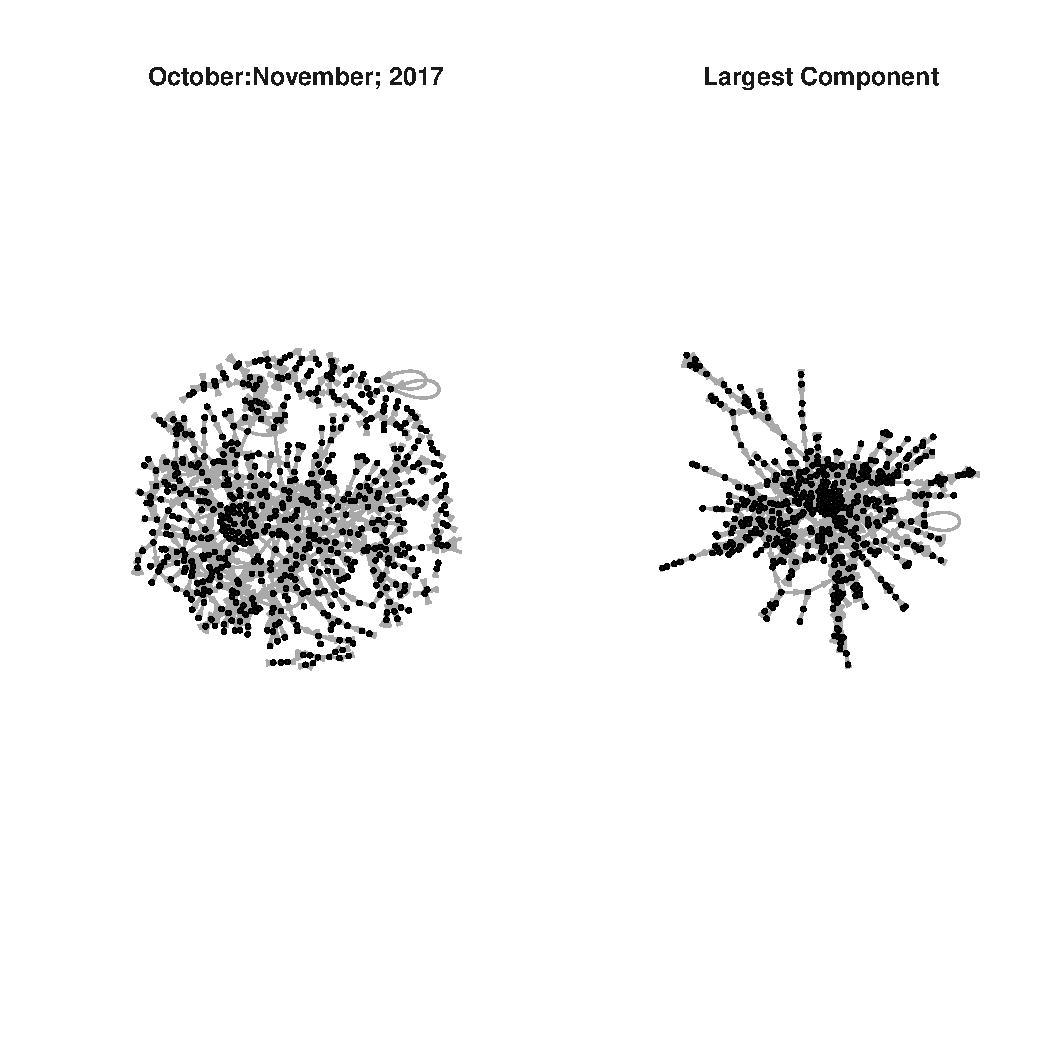
\includegraphics[width=6in]{figure/starting-1} 
\begin{kframe}\begin{alltt}
\hlstd{> }\hlkwd{par}\hlstd{(}\hlkwc{mfrow}\hlstd{=}\hlkwd{c}\hlstd{(}\hlnum{1}\hlstd{,}\hlnum{1}\hlstd{))}
\end{alltt}
\end{kframe}
\end{knitrout}
\end{center}

We can examine some measures of centrality from this network (using the full network instead of largest component). I'll calculate the degree, the inward degree, and outward degree. Then, I find the summary statistics and plot all of these in one concise plot.

\begin{center}
\begin{knitrout}
\definecolor{shadecolor}{rgb}{0.165, 0.169, 0.184}\color{fgcolor}\begin{kframe}
\begin{alltt}
\hlstd{> }\hlcom{# For this assignment, we are only interested in large component:}
\hlstd{> }\hlstd{graph.object} \hlkwb{<-} \hlstd{l.graph.object}
\hlstd{> }
\hlstd{> }\hlcom{# --}
\hlstd{> }\hlstd{degree} \hlkwb{<-} \hlkwd{degree}\hlstd{(graph.object)}
\hlstd{> }\hlstd{in.degree} \hlkwb{<-} \hlkwd{degree}\hlstd{(graph.object,} \hlkwc{mode}\hlstd{=}\hlstr{'in'}\hlstd{)}
\hlstd{> }\hlstd{out.degree} \hlkwb{<-} \hlkwd{degree}\hlstd{(graph.object,} \hlkwc{mode}\hlstd{=}\hlstr{'out'}\hlstd{)}
\hlstd{> }
\hlstd{> }\hlcom{# Summary Statistics:}
\hlstd{> }\hlkwd{summary}\hlstd{(out.degree)}
\end{alltt}
\begin{verbatim}
##    Min. 1st Qu.  Median    Mean 3rd Qu.    Max. 
##   0.000   1.000   1.000   1.859   2.000  58.000
\end{verbatim}
\begin{alltt}
\hlstd{> }\hlkwd{summary}\hlstd{(in.degree)}
\end{alltt}
\begin{verbatim}
##    Min. 1st Qu.  Median    Mean 3rd Qu.    Max. 
##   0.000   1.000   1.000   1.859   2.000  18.000
\end{verbatim}
\begin{alltt}
\hlstd{> }\hlkwd{summary}\hlstd{(degree)}
\end{alltt}
\begin{verbatim}
##    Min. 1st Qu.  Median    Mean 3rd Qu.    Max. 
##   1.000   1.000   2.000   3.718   4.000  65.000
\end{verbatim}
\begin{alltt}
\hlstd{> }\hlkwd{sd}\hlstd{(out.degree)}
\end{alltt}
\begin{verbatim}
## [1] 3.303878
\end{verbatim}
\begin{alltt}
\hlstd{> }\hlkwd{sd}\hlstd{(in.degree)}
\end{alltt}
\begin{verbatim}
## [1] 2.229811
\end{verbatim}
\begin{alltt}
\hlstd{> }\hlkwd{sd}\hlstd{(degree)}
\end{alltt}
\begin{verbatim}
## [1] 4.761777
\end{verbatim}
\begin{alltt}
\hlstd{> }\hlcom{# Grammar of Graphics:}
\hlstd{> }\hlkwd{library}\hlstd{(ggplot2)}
\hlstd{> }\hlkwd{library}\hlstd{(gridExtra)}
\hlstd{> }\hlkwd{library}\hlstd{(grid)}
\hlstd{> }
\hlstd{> }\hlstd{p1} \hlkwb{<-} \hlkwd{qplot}\hlstd{(out.degree)}\hlopt{+}
\hlstd{+ }     \hlkwd{theme_bw}\hlstd{()}\hlopt{+}
\hlstd{+ }     \hlkwd{xlab}\hlstd{(}\hlstr{"Outward Degree"}\hlstd{)}\hlopt{+}
\hlstd{+ }     \hlkwd{ylab}\hlstd{(}\hlstr{"N"}\hlstd{)}\hlopt{+}
\hlstd{+ }     \hlkwd{geom_vline}\hlstd{(}\hlkwc{xintercept}\hlstd{=}\hlnum{1.859}\hlstd{,} \hlkwc{linetype}\hlstd{=}\hlstr{"dashed"}\hlstd{)}\hlopt{+}
\hlstd{+ }     \hlkwd{annotate}\hlstd{(}\hlstr{"text"}\hlstd{,} \hlkwc{x} \hlstd{=} \hlnum{50}\hlstd{,} \hlkwc{y} \hlstd{=} \hlnum{400}\hlstd{,} \hlkwc{label} \hlstd{=} \hlstr{"sd = 3.30"}\hlstd{)}
\hlstd{> }
\hlstd{> }\hlstd{p2} \hlkwb{<-} \hlkwd{qplot}\hlstd{(in.degree)}\hlopt{+}
\hlstd{+ }     \hlkwd{theme_bw}\hlstd{()}\hlopt{+}
\hlstd{+ }     \hlkwd{xlab}\hlstd{(}\hlstr{"Inward Degree"}\hlstd{)}\hlopt{+}
\hlstd{+ }     \hlkwd{ylab}\hlstd{(}\hlstr{"N"}\hlstd{)}\hlopt{+}
\hlstd{+ }     \hlkwd{geom_vline}\hlstd{(}\hlkwc{xintercept}\hlstd{=}\hlnum{1.859}\hlstd{,} \hlkwc{linetype}\hlstd{=}\hlstr{"dashed"}\hlstd{)}\hlopt{+}
\hlstd{+ }     \hlkwd{annotate}\hlstd{(}\hlstr{"text"}\hlstd{,} \hlkwc{x} \hlstd{=} \hlnum{16}\hlstd{,} \hlkwc{y} \hlstd{=} \hlnum{213}\hlstd{,} \hlkwc{label} \hlstd{=} \hlstr{"sd = 2.23"}\hlstd{)}
\hlstd{> }
\hlstd{> }\hlstd{p3} \hlkwb{<-} \hlkwd{qplot}\hlstd{(degree)}\hlopt{+}
\hlstd{+ }     \hlkwd{theme_bw}\hlstd{()}\hlopt{+}
\hlstd{+ }     \hlkwd{xlab}\hlstd{(}\hlstr{"Degree"}\hlstd{)}\hlopt{+}
\hlstd{+ }     \hlkwd{ylab}\hlstd{(}\hlstr{"N"}\hlstd{)}\hlopt{+}
\hlstd{+ }     \hlkwd{geom_vline}\hlstd{(}\hlkwc{xintercept}\hlstd{=}\hlnum{3.718}\hlstd{,} \hlkwc{linetype}\hlstd{=}\hlstr{"dashed"}\hlstd{)}\hlopt{+}
\hlstd{+ }     \hlkwd{annotate}\hlstd{(}\hlstr{"text"}\hlstd{,} \hlkwc{x} \hlstd{=} \hlnum{61}\hlstd{,} \hlkwc{y} \hlstd{=} \hlnum{214}\hlstd{,} \hlkwc{label} \hlstd{=} \hlstr{"sd = 4.76"}\hlstd{)}
\hlstd{> }
\hlstd{> }\hlkwd{grid.arrange}\hlstd{(}
\hlstd{+ }     \hlstd{p1, p2, p3,}
\hlstd{+ }     \hlcom{# Graphing Matrix:}
\hlstd{+ }     \hlkwc{widths} \hlstd{=} \hlkwd{c}\hlstd{(}\hlnum{.5}\hlstd{,} \hlnum{.9} \hlstd{,}\hlnum{2}\hlstd{,} \hlnum{2}\hlstd{,} \hlnum{.9}\hlstd{,} \hlnum{.5}\hlstd{),}
\hlstd{+ }     \hlkwc{layout_matrix} \hlstd{=} \hlkwd{rbind}\hlstd{(}\hlkwd{c}\hlstd{(}\hlnum{NA}\hlstd{,} \hlnum{1}\hlstd{,} \hlnum{1}\hlstd{,} \hlnum{2}\hlstd{,} \hlnum{2}\hlstd{,} \hlnum{NA}\hlstd{),}
\hlstd{+ }                           \hlkwd{c}\hlstd{(}\hlnum{NA}\hlstd{,} \hlnum{NA}\hlstd{,} \hlnum{3}\hlstd{,} \hlnum{3}\hlstd{,} \hlnum{NA}\hlstd{,} \hlnum{NA}\hlstd{)),}
\hlstd{+ }     \hlkwc{top} \hlstd{=} \hlstr{"Network Degree Distributions;
          \textbackslash{}n Oct : Nov'r/AskSocialScientists' Reddit Data."}\hlstd{,}
\hlstd{+ }     \hlcom{# Any citations:}
\hlstd{+ }     \hlkwc{bottom} \hlstd{=} \hlkwd{textGrob}\hlstd{(}
\hlstd{+ }          \hlstr{"Mean Reported by Dashed Line.
          \textbackslash{}n All Medians = 1 except 'Degree' which = 2 "}\hlstd{,}
\hlstd{+ }          \hlkwc{gp} \hlstd{=} \hlkwd{gpar}\hlstd{(}\hlkwc{fontface} \hlstd{=} \hlnum{3}\hlstd{,} \hlkwc{fontsize} \hlstd{=} \hlnum{8}\hlstd{),}
\hlstd{+ }          \hlkwc{hjust} \hlstd{=} \hlnum{1}\hlstd{,}
\hlstd{+ }          \hlkwc{x} \hlstd{=} \hlnum{1}
\hlstd{+ }     \hlstd{)}
\hlstd{+ }\hlstd{)}
\end{alltt}
\end{kframe}
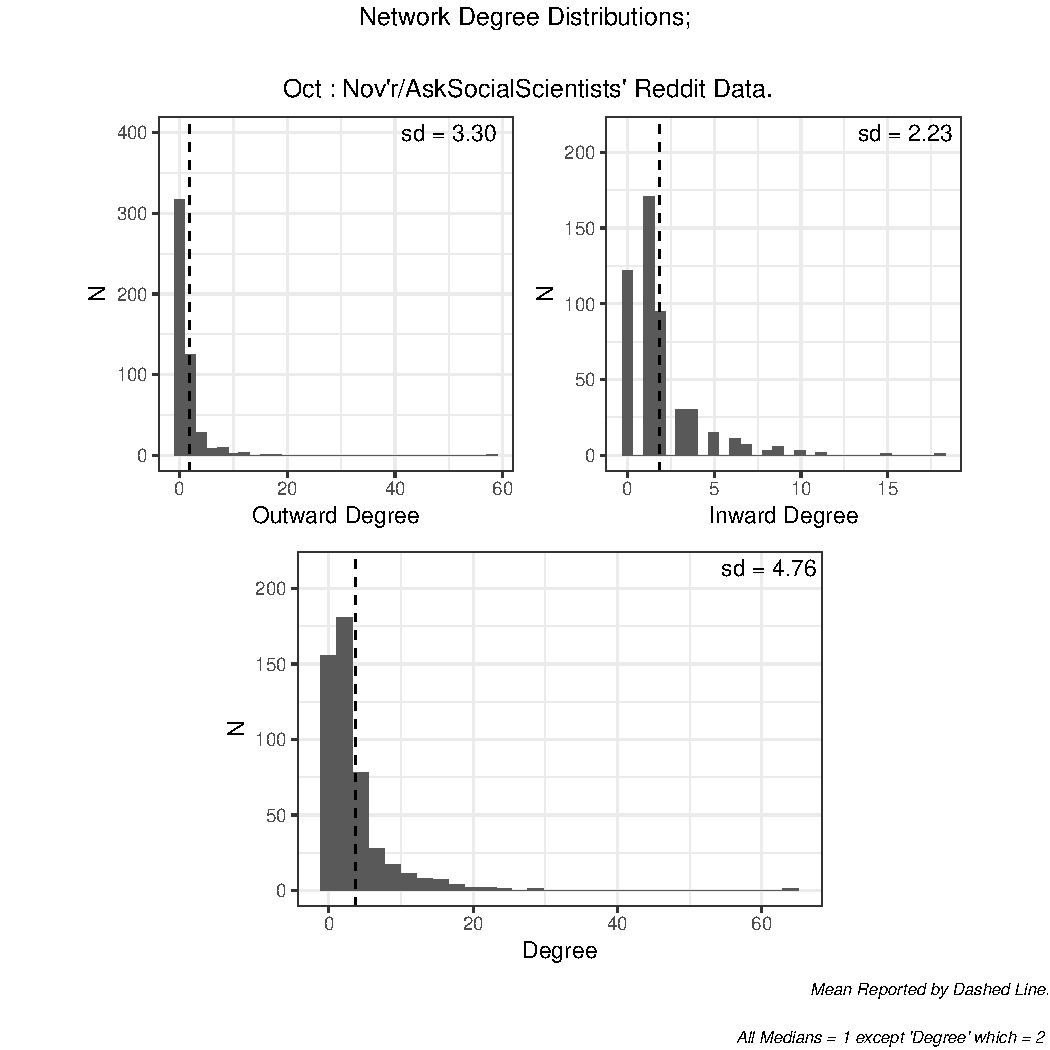
\includegraphics[width=6in]{figure/degree-1} 

\end{knitrout}
\end{center}


The next part was difficult, and probably could be done better. I looked at a list of the ordered centrality measures, then created an edge-graph and looked at those lists similarly. We can see from the lists that some names pop up more often then others (MoralMidgetry, apaniyam, Atriox998), but there has to be some code to get the ``max'' or to highlight those with the largest degree more clearly. How might we code that? \index{ggplot}

\begin{knitrout}
\definecolor{shadecolor}{rgb}{0.165, 0.169, 0.184}\color{fgcolor}\begin{kframe}
\begin{alltt}
\hlstd{> }\hlcom{### Centrality measures:}
\hlstd{> }\hlstd{lg_graph.object} \hlkwb{<-} \hlkwd{line.graph}\hlstd{(graph.object)}
\hlstd{> }
\hlstd{> }\hlcom{## closeness centrality}
\hlstd{> }\hlstd{c.graph.object} \hlkwb{<-} \hlkwd{closeness}\hlstd{(graph.object)}
\hlstd{> }\hlkwd{summary}\hlstd{(c.graph.object)}
\end{alltt}
\begin{verbatim}
##      Min.   1st Qu.    Median      Mean   3rd Qu.      Max. 
## 4.057e-06 4.065e-06 4.165e-06 5.800e-06 8.021e-06 8.439e-06
\end{verbatim}
\begin{alltt}
\hlstd{> }\hlkwd{E}\hlstd{(graph.object)[}\hlkwd{order}\hlstd{(c.graph.object,} \hlkwc{decreasing}\hlstd{=T)[}\hlnum{1}\hlopt{:}\hlnum{10}\hlstd{]]}
\end{alltt}
\begin{verbatim}
## + 10/924 edges from 26bfaac (vertex names):
##  [1] yodatsracist       ->dewarr   SpecificallyGeneral->gacorley
##  [3] inh-uman           ->gacorley Shazbot_Nanu       ->Ramicus 
##  [5] Mentalpopcorn      ->PeechMan Drict              ->USMCLee 
##  [7] apaniyam           ->faguzzi  ExpectedSurprisal  ->sverdo  
##  [9] UpsideVII          ->apaniyam VincentStaples     ->sverdo
\end{verbatim}
\begin{alltt}
\hlstd{> }\hlstd{c.lg.graph.object} \hlkwb{<-} \hlkwd{closeness}\hlstd{(lg_graph.object)}
\hlstd{> }\hlkwd{E}\hlstd{(graph.object)[}\hlkwd{order}\hlstd{(c.lg.graph.object,} \hlkwc{decreasing}\hlstd{=T)[}\hlnum{1}\hlopt{:}\hlnum{10}\hlstd{]]}
\end{alltt}
\begin{verbatim}
## + 10/924 edges from 26bfaac (vertex names):
##  [1] Atriox998         ->wellmanicuredman  
##  [2] Galileotierraplana->Atriox998         
##  [3] wellmanicuredman  ->Atriox998         
##  [4] Atriox998         ->Galileotierraplana
##  [5] dmoni002          ->UpsideVII         
##  [6] UpsideVII         ->apaniyam          
##  [7] thatgerhard       ->apaniyam          
##  [8] Cyllya            ->siali             
##  [9] faguzzi           ->apaniyam          
## [10] siali             ->apaniyam
\end{verbatim}
\begin{alltt}
\hlstd{> }\hlcom{## betweenness centrality}
\hlstd{> }\hlstd{b.graph.object} \hlkwb{<-} \hlkwd{betweenness}\hlstd{(graph.object)}
\hlstd{> }\hlkwd{summary}\hlstd{(b.graph.object)}
\end{alltt}
\begin{verbatim}
##    Min. 1st Qu.  Median    Mean 3rd Qu.    Max. 
##     0.0     0.0     0.0   868.9   227.0 29810.0
\end{verbatim}
\begin{alltt}
\hlstd{> }\hlkwd{E}\hlstd{(graph.object)[}\hlkwd{order}\hlstd{(b.graph.object,} \hlkwc{decreasing}\hlstd{=T)[}\hlnum{1}\hlopt{:}\hlnum{10}\hlstd{]]}
\end{alltt}
\begin{verbatim}
## + 10/924 edges from 26bfaac (vertex names):
##  [1] sambalchuck     ->orthag             
##  [2] DarkGamer       ->Cullen_Ingus       
##  [3] obamanisha      ->Aquifex            
##  [4] PLEASE_USE_LOGIC->LD_in_MT           
##  [5] TychoCelchuuu   ->Traz_Onmale        
##  [6] sverdo          ->racornist          
##  [7] owlpellet       ->sverdo             
##  [8] obamanisha      ->North_London_Gunner
##  [9] benjaminikuta   ->Klumber            
## [10] TychoCelchuuu   ->Traz_Onmale
\end{verbatim}
\begin{alltt}
\hlstd{> }\hlstd{b.lg.graph.object} \hlkwb{<-} \hlkwd{betweenness}\hlstd{(lg_graph.object)}
\hlstd{> }\hlkwd{E}\hlstd{(graph.object)[}\hlkwd{order}\hlstd{(b.lg.graph.object,} \hlkwc{decreasing}\hlstd{=T)[}\hlnum{1}\hlopt{:}\hlnum{10}\hlstd{]]}
\end{alltt}
\begin{verbatim}
## + 10/924 edges from 26bfaac (vertex names):
##  [1] yodatsracist  ->Randomname64   Fibonacci35813->deathlock13   
##  [3] vulcan583     ->Fibonacci35813 Erinaceous    ->vulcan583     
##  [5] dewarr        ->yodatsracist   Randomname64  ->Erinaceous    
##  [7] Randomname64  ->Erinaceous     morpheusx66   ->dewarr        
##  [9] Erinaceous    ->isntanywhere   isntanywhere  ->Snugglerific
\end{verbatim}
\begin{alltt}
\hlstd{> }\hlcom{## eigenvector centrality}
\hlstd{> }\hlstd{e.graph.object} \hlkwb{<-} \hlkwd{evcent}\hlstd{(graph.object)}
\hlstd{> }\hlkwd{summary}\hlstd{(e.graph.object}\hlopt{$}\hlstd{vector)}
\end{alltt}
\begin{verbatim}
##     Min.  1st Qu.   Median     Mean  3rd Qu.     Max. 
## 0.00e+00 5.50e-06 5.67e-05 9.94e-03 4.66e-04 1.00e+00
\end{verbatim}
\begin{alltt}
\hlstd{> }\hlkwd{E}\hlstd{(graph.object)[}\hlkwd{order}\hlstd{(e.graph.object}\hlopt{$}\hlstd{vector,} \hlkwc{decreasing}\hlstd{=T)[}\hlnum{1}\hlopt{:}\hlnum{10}\hlstd{]]}
\end{alltt}
\begin{verbatim}
## + 10/924 edges from 26bfaac (vertex names):
##  [1] MoralMidgetry  ->Dumble_dared        just_works_here->PM_ME_YOUR_SHEC0CK 
##  [3] timeimmemorial ->dewarr              Kai_Daigoji    ->Klumber            
##  [5] sambalchuck    ->orthag              HerrtomtomAZ   ->Newnews2           
##  [7] inh-uman       ->chroboo             emptynothing   ->sambalchuck        
##  [9] Klumber        ->NoFascistAgreements nllanki        ->Klumber
\end{verbatim}
\begin{alltt}
\hlstd{> }\hlstd{evc_lg_graph.object} \hlkwb{<-} \hlkwd{evcent}\hlstd{(lg_graph.object)}
\hlstd{> }\hlkwd{E}\hlstd{(graph.object)[}\hlkwd{order}\hlstd{(evc_lg_graph.object}\hlopt{$}\hlstd{vector,} \hlkwc{decreasing}\hlstd{=T)[}\hlnum{1}\hlopt{:}\hlnum{10}\hlstd{]]}
\end{alltt}
\begin{verbatim}
## + 10/924 edges from 26bfaac (vertex names):
##  [1] Dennis_Langley  ->MoralMidgetry  Dennis_Langley  ->MoralMidgetry 
##  [3] Dennis_Langley  ->MoralMidgetry  deathlock13     ->MoralMidgetry 
##  [5] deathlock13     ->MoralMidgetry  BuildBetterWorld->MoralMidgetry 
##  [7] lafayette0508   ->MoralMidgetry  MoralMidgetry   ->Dennis_Langley
##  [9] MoralMidgetry   ->Dennis_Langley MoralMidgetry   ->Dennis_Langley
\end{verbatim}
\end{kframe}
\end{knitrout}


At least from above we know where to start looking for central nodes within our data. Following this, I compare each measure of centrality by generating a matrix of correlation values, then plot it.

\begin{center}
\begin{knitrout}
\definecolor{shadecolor}{rgb}{0.165, 0.169, 0.184}\color{fgcolor}\begin{kframe}
\begin{alltt}
\hlstd{> }\hlcom{# Let's whip-up a matrix of just our values, look at the correlation between them.}
\hlstd{> }\hlstd{vec.degree} \hlkwb{<-} \hlkwd{as.vector}\hlstd{(degree)}
\hlstd{> }\hlstd{vec.in.degree} \hlkwb{<-} \hlkwd{as.vector}\hlstd{(in.degree)}
\hlstd{> }\hlstd{vec.out.degree} \hlkwb{<-} \hlkwd{as.vector}\hlstd{(out.degree)}
\hlstd{> }\hlstd{vec.c.graph.object} \hlkwb{<-} \hlkwd{as.vector}\hlstd{(c.graph.object)}
\hlstd{> }\hlstd{vec.b.graph.object} \hlkwb{<-} \hlkwd{as.vector}\hlstd{(b.graph.object)}
\hlstd{> }\hlstd{vec.e.graph.object} \hlkwb{<-} \hlkwd{as.vector}\hlstd{(e.graph.object}\hlopt{$}\hlstd{vector)}
\hlstd{> }
\hlstd{> }
\hlstd{> }\hlstd{Cor.Object} \hlkwb{<-} \hlkwd{matrix}\hlstd{(}\hlkwd{c}\hlstd{(vec.degree, vec.in.degree, vec.out.degree,}
\hlstd{+ }                       \hlstd{vec.c.graph.object, vec.b.graph.object, vec.e.graph.object),}
\hlstd{+ }                      \hlkwc{ncol}\hlstd{=}\hlnum{6}\hlstd{)}
\hlstd{> }
\hlstd{> }\hlkwd{colnames}\hlstd{(Cor.Object)} \hlkwb{<-} \hlkwd{c}\hlstd{(}\hlstr{"Degree"}\hlstd{,} \hlstr{"In Degree"}\hlstd{,} \hlstr{"Out Degree"}\hlstd{,}
\hlstd{+ }                         \hlstr{"Closeness"}\hlstd{,} \hlstr{"Betweeness"}\hlstd{,} \hlstr{"Eigenvector"}\hlstd{)}
\hlstd{> }
\hlstd{> }\hlkwd{cor}\hlstd{(Cor.Object)}
\end{alltt}
\begin{verbatim}
##                Degree In Degree Out Degree  Closeness  Betweeness Eigenvector
## Degree      1.0000000 0.7878691  0.9095307  0.2354144  0.60688044  0.22276886
## In Degree   0.7878691 1.0000000  0.4606242  0.1250300  0.50376591  0.25588522
## Out Degree  0.9095307 0.4606242  1.0000000  0.2549119  0.53468285  0.14837111
## Closeness   0.2354144 0.1250300  0.2549119  1.0000000  0.28440051 -0.10317000
## Betweeness  0.6068804 0.5037659  0.5346828  0.2844005  1.00000000 -0.02671278
## Eigenvector 0.2227689 0.2558852  0.1483711 -0.1031700 -0.02671278  1.00000000
\end{verbatim}
\begin{alltt}
\hlstd{> }\hlcom{# Trying to think of cool ways to plot this:}
\hlstd{> }\hlkwd{library}\hlstd{(corrplot)}
\hlstd{> }\hlstd{x} \hlkwb{<-} \hlkwd{cor}\hlstd{(Cor.Object)}
\hlstd{> }\hlkwd{corrplot}\hlstd{(x,} \hlkwc{type}\hlstd{=}\hlstr{"upper"}\hlstd{,} \hlkwc{order}\hlstd{=}\hlstr{"hclust"}\hlstd{)}
\end{alltt}
\end{kframe}
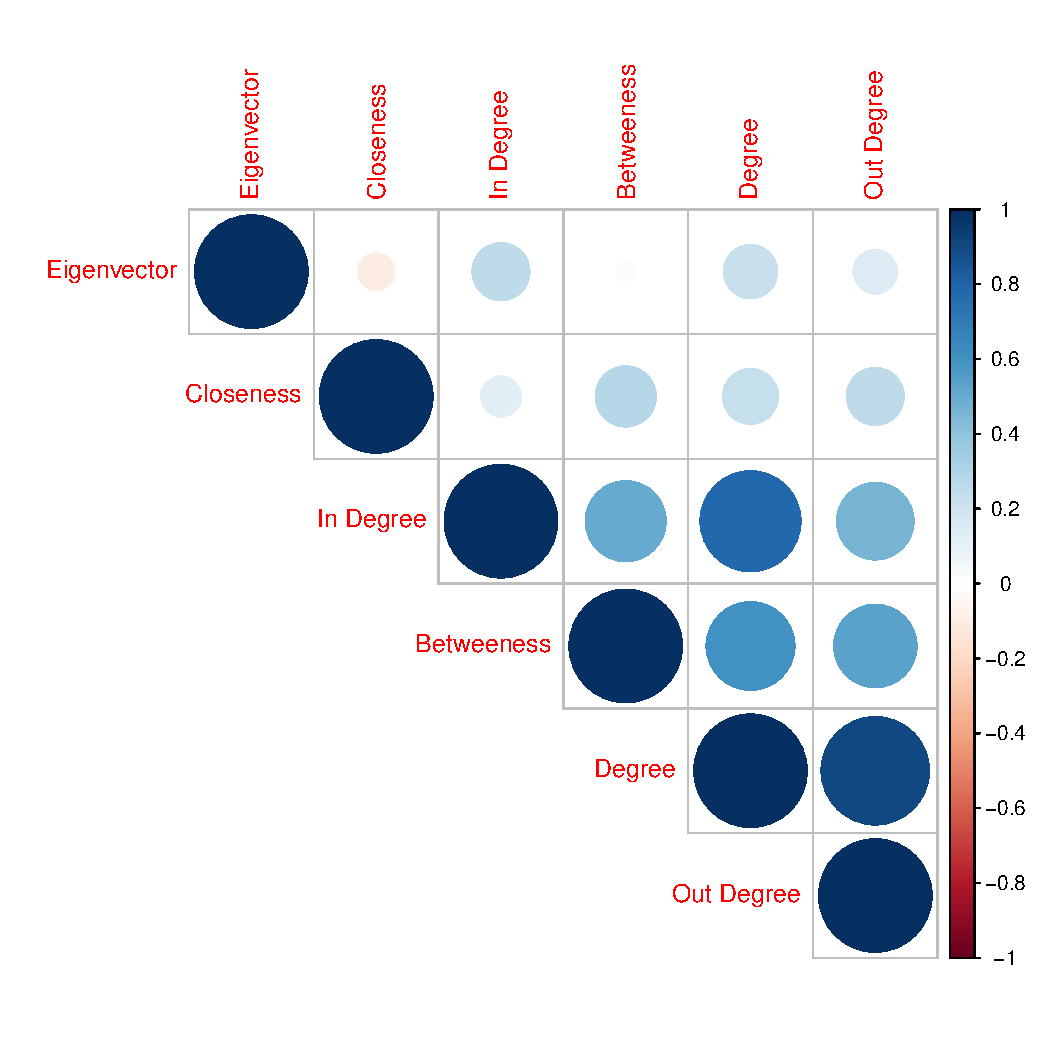
\includegraphics[width=6in]{figure/comp-1} 

\end{knitrout}
\end{center}


I find it easier to think about correlation by looking at the plot (albiet a very rough plot). The two ``darkest'' or most correlated measures was the in-degree with degree, and the degree with the out-degree. This makes sense because the degree is encapsulating both of those measures. All measures are positively correlated, except the eigenvector centrality measure compared to closeness and betweeness. This is likely because of the different assumptions and properties each of these measures have. For example, eigenvector centrality Trafic moves along unrestricted walks, Trafic can effect subsequent nodes simultaneously, and eigenvector centrality measures long-term and indirect risks. Other measures may not have these properties, so it is probably best that they are not too closely correlated.


%--------------------------------------
\subsubsection{Data Viz}

Perhpas now is a good opportunity to talk about data vizualisation. Using the data from the previous section on centrality:
In this I will be using the Reddit data from "r/AskSocialScientists" from October and November. These will be ran seperately, and I will look into their largest components. Then, I will plot the degrees in two different ways.

\begin{knitrout}
\definecolor{shadecolor}{rgb}{0.165, 0.169, 0.184}\color{fgcolor}\begin{kframe}
\begin{alltt}
\hlstd{> }\hlcom{# Using the data set up from the previous section:}
\hlstd{> }\hlcom{##    Oct:}
\hlstd{> }\hlkwd{library}\hlstd{(igraph)}
\hlstd{> }\hlstd{g1} \hlkwb{<-} \hlkwd{graph_from_edgelist}\hlstd{(el)}
\hlstd{> }\hlkwd{summary}\hlstd{(g1)} \hlcom{#}
\end{alltt}
\begin{verbatim}
## IGRAPH 2a72c36 DN-- 339 521 -- 
## + attr: name (v/c)
\end{verbatim}
\begin{alltt}
\hlstd{> }\hlcom{#---------------------------------------------------------------------------}
\hlstd{> }\hlcom{##   Nov:}
\hlstd{> }\hlstd{g12} \hlkwb{<-} \hlkwd{graph_from_edgelist}\hlstd{(el2)}
\hlstd{> }\hlkwd{summary}\hlstd{(g12)} \hlcom{#}
\end{alltt}
\begin{verbatim}
## IGRAPH 2a73aca DN-- 327 522 -- 
## + attr: name (v/c)
\end{verbatim}
\end{kframe}
\end{knitrout}

\begin{center}
\begin{knitrout}
\definecolor{shadecolor}{rgb}{0.165, 0.169, 0.184}\color{fgcolor}\begin{kframe}
\begin{alltt}
\hlstd{> }\hlkwd{set.seed}\hlstd{(}\hlnum{8675309}\hlstd{)}  \hlcom{# 1981 throwback seed}
\hlstd{> }
\hlstd{> }\hlkwd{par}\hlstd{(}\hlkwc{mfrow}\hlstd{=}\hlkwd{c}\hlstd{(}\hlnum{1}\hlstd{,}\hlnum{2}\hlstd{))}
\hlstd{> }\hlkwd{plot.igraph}\hlstd{(g1,}
\hlstd{+ }            \hlkwc{vertex.color}\hlstd{=}\hlstr{"gray15"}\hlstd{,}
\hlstd{+ }            \hlkwc{vertex.size}\hlstd{=}\hlnum{2.7}\hlstd{,}
\hlstd{+ }            \hlkwc{vertex.label}\hlstd{=}\hlnum{NA}\hlstd{,}
\hlstd{+ }            \hlkwc{vertex.shape}\hlstd{=}\hlstr{"circle"}\hlstd{,}
\hlstd{+ }            \hlkwc{edge.arrow.size}\hlstd{=}\hlnum{0.4}\hlstd{,}
\hlstd{+ }            \hlkwc{edge.arrow.width}\hlstd{=}\hlnum{.6}\hlstd{,}
\hlstd{+ }            \hlkwc{edge.width}\hlstd{=}\hlnum{1.5}\hlstd{)}
\hlstd{> }\hlkwd{title}\hlstd{(}\hlstr{"\textbackslash{}n October; 2017"}\hlstd{,}
\hlstd{+ }      \hlkwc{cex.main}\hlstd{=}\hlnum{1}\hlstd{,} \hlkwc{col.main}\hlstd{=}\hlstr{"gray10"}\hlstd{)}
\hlstd{> }
\hlstd{> }\hlkwd{plot.igraph}\hlstd{(g12,}
\hlstd{+ }            \hlkwc{vertex.color}\hlstd{=}\hlstr{"gray15"}\hlstd{,}
\hlstd{+ }            \hlkwc{vertex.size}\hlstd{=}\hlnum{2.7}\hlstd{,}
\hlstd{+ }            \hlkwc{vertex.label}\hlstd{=}\hlnum{NA}\hlstd{,}
\hlstd{+ }            \hlkwc{vertex.shape}\hlstd{=}\hlstr{"circle"}\hlstd{,}
\hlstd{+ }            \hlkwc{edge.arrow.size}\hlstd{=}\hlnum{0.4}\hlstd{,}
\hlstd{+ }            \hlkwc{edge.arrow.width}\hlstd{=}\hlnum{.6}\hlstd{,}
\hlstd{+ }            \hlkwc{edge.width}\hlstd{=}\hlnum{1.5}\hlstd{)}
\hlstd{> }\hlkwd{title}\hlstd{(}\hlstr{"\textbackslash{}n November; 2017"}\hlstd{,}
\hlstd{+ }      \hlkwc{cex.main}\hlstd{=}\hlnum{1}\hlstd{,} \hlkwc{col.main}\hlstd{=}\hlstr{"gray10"}\hlstd{)}
\end{alltt}
\end{kframe}
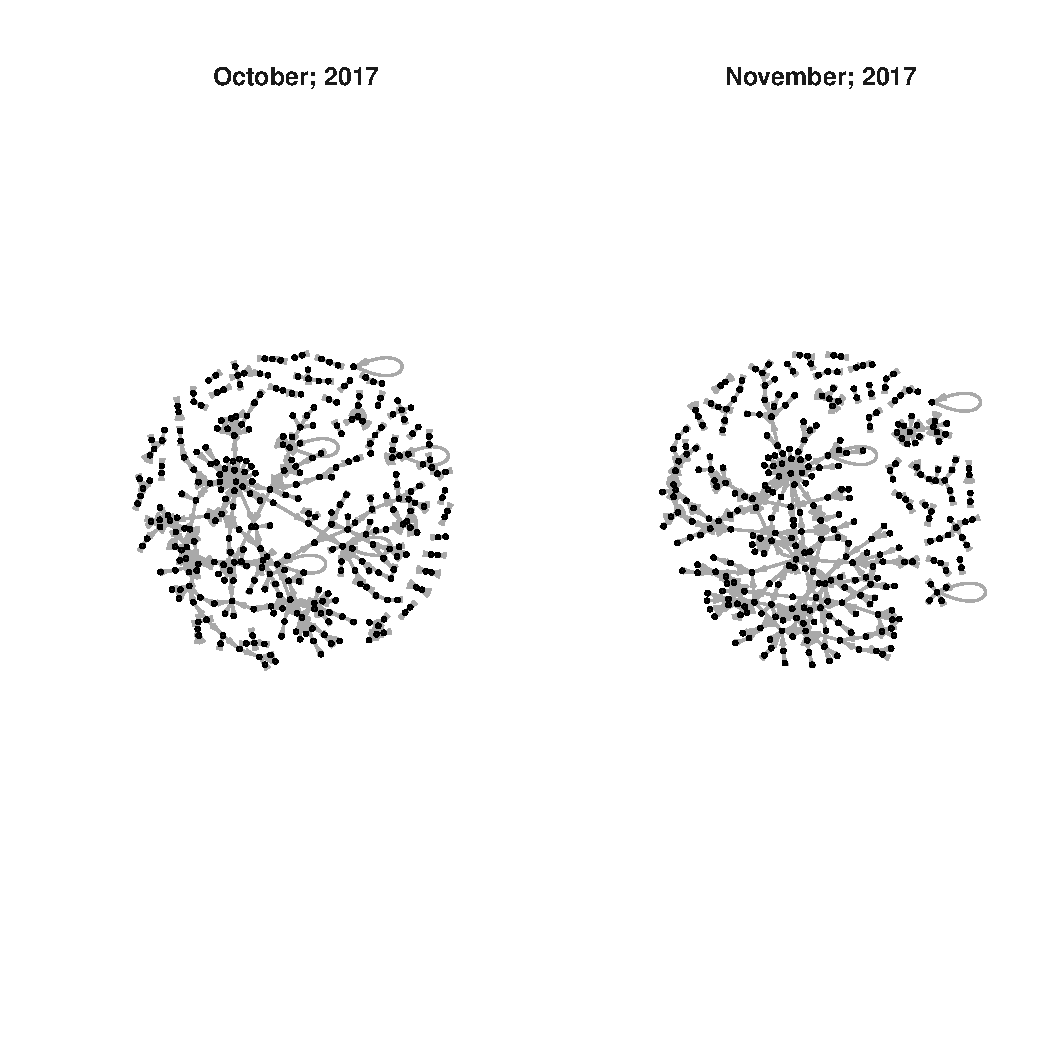
\includegraphics[width=5in]{figure/plot1-1} 
\begin{kframe}\begin{alltt}
\hlstd{> }\hlkwd{par}\hlstd{(}\hlkwc{mfrow}\hlstd{=}\hlkwd{c}\hlstd{(}\hlnum{1}\hlstd{,}\hlnum{1}\hlstd{))} \hlcom{# basic reset}
\end{alltt}
\end{kframe}
\end{knitrout}
\end{center}

Above we have both of our complete networks for both months. In these graphs we simply have users (nodes) and if they have commented on each other's posts (edges). This may include some information that is less interesting, like users that have no comments. Below we will take the two largest components of each network and plot it.

\begin{center}
\begin{knitrout}
\definecolor{shadecolor}{rgb}{0.165, 0.169, 0.184}\color{fgcolor}\begin{kframe}
\begin{alltt}
\hlstd{> }\hlstd{giant.component} \hlkwb{<-} \hlkwa{function}\hlstd{(}\hlkwc{graph}\hlstd{) \{}
\hlstd{+ }     \hlstd{cl} \hlkwb{<-} \hlkwd{clusters}\hlstd{(graph)}
\hlstd{+ }     \hlkwd{induced.subgraph}\hlstd{(graph,} \hlkwd{which}\hlstd{(cl}\hlopt{$}\hlstd{membership} \hlopt{==} \hlkwd{which.max}\hlstd{(cl}\hlopt{$}\hlstd{csize)))}
\hlstd{+ }\hlstd{\}}
\hlstd{> }
\hlstd{> }\hlstd{g2} \hlkwb{<-} \hlkwd{giant.component}\hlstd{(g1)}
\hlstd{> }\hlstd{g22} \hlkwb{<-} \hlkwd{giant.component}\hlstd{(g12)}
\hlstd{> }
\hlstd{> }
\hlstd{> }\hlkwd{par}\hlstd{(}\hlkwc{mfrow}\hlstd{=}\hlkwd{c}\hlstd{(}\hlnum{1}\hlstd{,}\hlnum{2}\hlstd{))}
\hlstd{> }\hlkwd{plot.igraph}\hlstd{(g2,}
\hlstd{+ }            \hlkwc{vertex.color}\hlstd{=}\hlstr{"gray15"}\hlstd{,}
\hlstd{+ }            \hlkwc{vertex.size}\hlstd{=}\hlnum{2.7}\hlstd{,}
\hlstd{+ }            \hlkwc{vertex.label}\hlstd{=}\hlnum{NA}\hlstd{,}
\hlstd{+ }            \hlkwc{vertex.shape}\hlstd{=}\hlstr{"circle"}\hlstd{,}
\hlstd{+ }            \hlkwc{edge.arrow.size}\hlstd{=}\hlnum{0.4}\hlstd{,}
\hlstd{+ }            \hlkwc{edge.arrow.width}\hlstd{=}\hlnum{.6}\hlstd{,}
\hlstd{+ }            \hlkwc{edge.width}\hlstd{=}\hlnum{1.5}\hlstd{)}
\hlstd{> }\hlkwd{title}\hlstd{(}\hlstr{"\textbackslash{}n October; 2017"}\hlstd{,}
\hlstd{+ }      \hlkwc{cex.main}\hlstd{=}\hlnum{1}\hlstd{,} \hlkwc{col.main}\hlstd{=}\hlstr{"gray10"}\hlstd{)}
\hlstd{> }
\hlstd{> }\hlkwd{plot.igraph}\hlstd{(g22,}
\hlstd{+ }            \hlkwc{vertex.color}\hlstd{=}\hlstr{"gray15"}\hlstd{,}
\hlstd{+ }            \hlkwc{vertex.size}\hlstd{=}\hlnum{2.7}\hlstd{,}
\hlstd{+ }            \hlkwc{vertex.label}\hlstd{=}\hlnum{NA}\hlstd{,}
\hlstd{+ }            \hlkwc{vertex.shape}\hlstd{=}\hlstr{"circle"}\hlstd{,}
\hlstd{+ }            \hlkwc{edge.arrow.size}\hlstd{=}\hlnum{0.4}\hlstd{,}
\hlstd{+ }            \hlkwc{edge.arrow.width}\hlstd{=}\hlnum{.6}\hlstd{,}
\hlstd{+ }            \hlkwc{edge.width}\hlstd{=}\hlnum{1.5}\hlstd{)}
\hlstd{> }\hlkwd{title}\hlstd{(}\hlstr{"\textbackslash{}n November; 2017"}\hlstd{,}
\hlstd{+ }      \hlkwc{cex.main}\hlstd{=}\hlnum{1}\hlstd{,} \hlkwc{col.main}\hlstd{=}\hlstr{"gray10"}\hlstd{)}
\end{alltt}
\end{kframe}
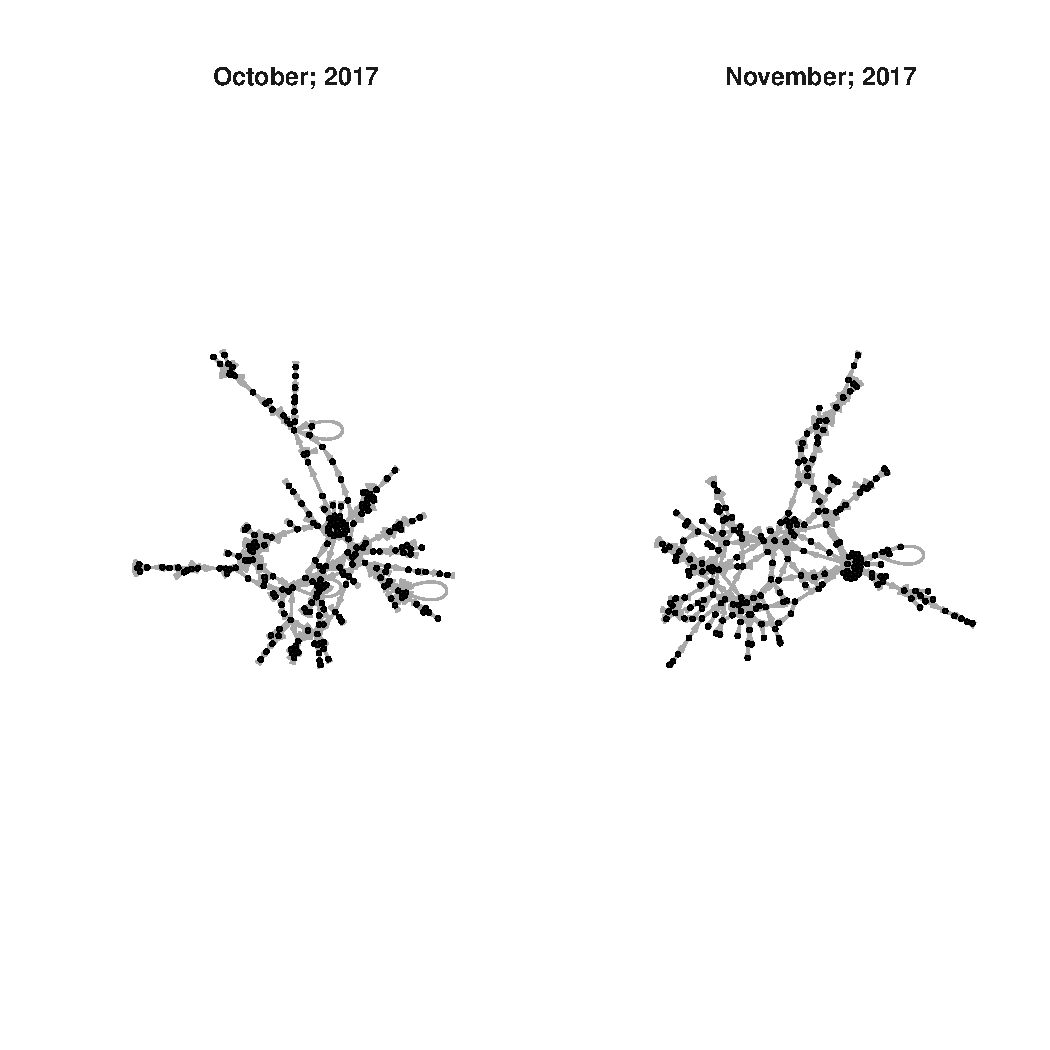
\includegraphics[width=5in]{figure/plot2-1} 

\end{knitrout}
\end{center}

For the above, I have chosen to keep plots simple and not too complex to overcomplicate interpretation. In a paper these graphs would likely print and be easily read. Some things that I may consider chaning is making the network bigger, and to have directionality more clear.\\

This is, of course, not the only information we can gain from a network. Below is a plot of the network degrees. A network "degree" is the number of connections each node has - a useful statistic. The following graphs intended purpose is to report the mean, the nodes, and edges in addition to the distribution of degrees in a network.

\begin{center}
\begin{knitrout}
\definecolor{shadecolor}{rgb}{0.165, 0.169, 0.184}\color{fgcolor}\begin{kframe}
\begin{alltt}
\hlstd{> }\hlstd{Degree} \hlkwb{<-} \hlkwd{degree}\hlstd{(g2)}
\hlstd{> }\hlkwd{mean}\hlstd{(Degree)}
\end{alltt}
\begin{verbatim}
## [1] 3.497835
\end{verbatim}
\begin{alltt}
\hlstd{> }\hlkwd{library}\hlstd{(ggplot2)}
\hlstd{> }\hlkwd{qplot}\hlstd{(Degree)}\hlopt{+}
\hlstd{+ }     \hlkwd{theme_bw}\hlstd{()}\hlopt{+}
\hlstd{+ }     \hlkwd{ylab}\hlstd{(}\hlstr{"N"}\hlstd{)}\hlopt{+}
\hlstd{+ }     \hlkwd{xlab}\hlstd{(}\hlstr{"Degrees"}\hlstd{)}\hlopt{+}
\hlstd{+ }     \hlcom{#ggtitle("Degrees in Large Component of Network 1")+}
\hlstd{+ }     \hlkwd{ggtitle}\hlstd{(}\hlkwd{substitute}\hlstd{(}
\hlstd{+ }          \hlkwd{paste}\hlstd{(} \hlstr{"Large Component Degrees, with: "}\hlstd{, N[V],} \hlstr{"="}\hlstd{,} \hlnum{231}\hlstd{,}
\hlstd{+ }                 \hlstr{" and "}\hlstd{, N[E],} \hlstr{"="}\hlstd{,} \hlnum{404}\hlstd{)))}\hlopt{+}
\hlstd{+ }     \hlkwd{annotate}\hlstd{(}\hlstr{"text"}\hlstd{,} \hlkwc{x} \hlstd{=} \hlnum{35.4}\hlstd{,} \hlkwc{y} \hlstd{=} \hlnum{3.7}\hlstd{,} \hlkwc{label} \hlstd{=} \hlstr{"35"}\hlstd{)}\hlopt{+}
\hlstd{+ }     \hlkwd{geom_vline}\hlstd{(}\hlkwc{xintercept}\hlstd{=}\hlkwd{mean}\hlstd{(Degree),} \hlkwc{linetype}\hlstd{=}\hlstr{"dashed"}\hlstd{)}\hlopt{+}
\hlstd{+ }     \hlkwd{annotate}\hlstd{(}\hlstr{"text"}\hlstd{,} \hlkwc{x} \hlstd{=} \hlnum{4.3}\hlstd{,} \hlkwc{y} \hlstd{=} \hlnum{71}\hlstd{,} \hlkwc{label} \hlstd{=} \hlkwd{round}\hlstd{(}\hlkwd{mean}\hlstd{(Degree),}\hlnum{3}\hlstd{),} \hlkwc{angle}\hlstd{=}\hlopt{-}\hlnum{90}\hlstd{)}
\end{alltt}
\end{kframe}
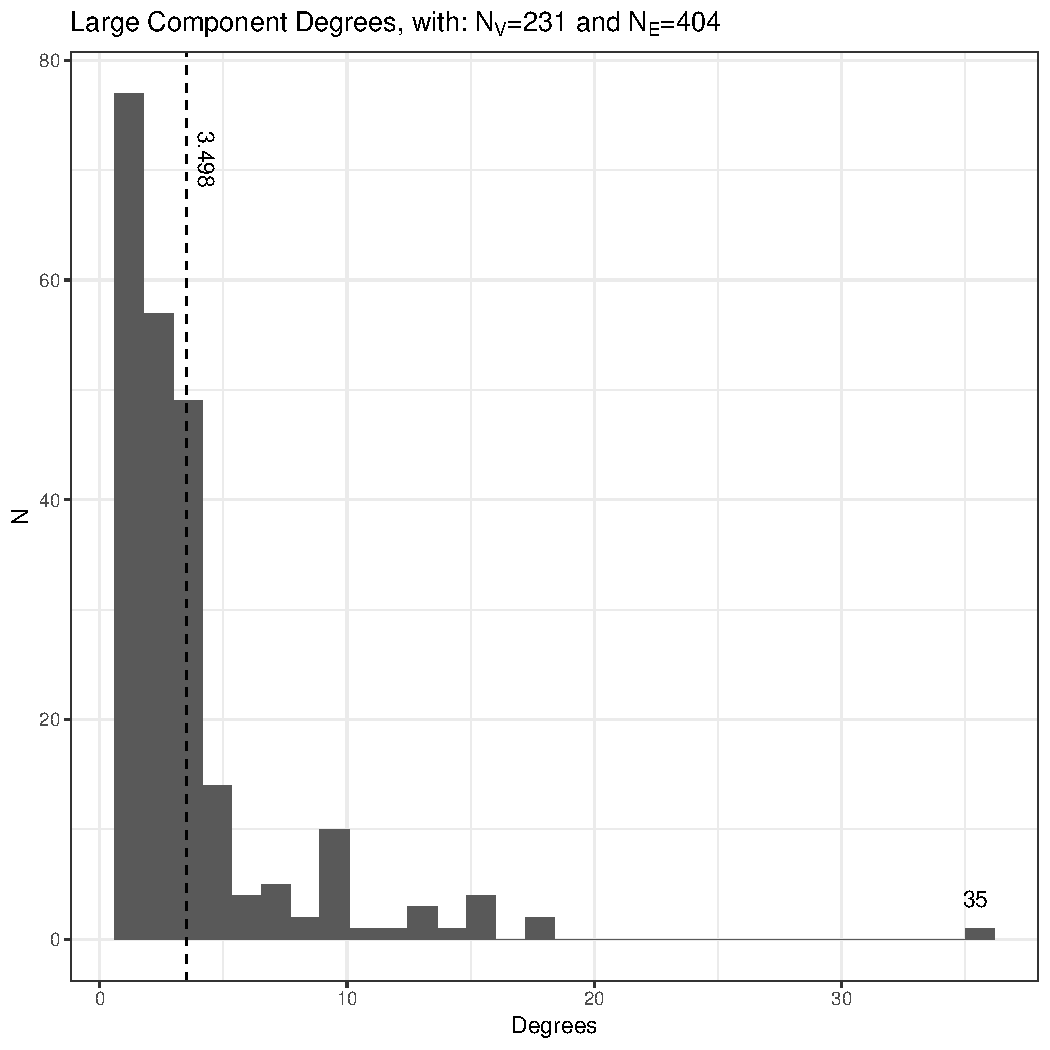
\includegraphics[width=5in]{figure/plot3-1} 

\end{knitrout}
\end{center}

We might be interested in the same network statistic but reported with the help of feline friends. Certainly journals today would not accept this, but perhaps they will someday when the job market slows down. Below is a ``CatterPlot'' of the degrees in our network, cats are in two colors to better show distinction. Note the clowder of cats in the lower-degree levels and the one cat in the top left being the most ``social'' in our Reddit data. One advantage to a plot like this could be how it attracts the reader and adds a element of humor; however, the plot could be easily distracting and obnoxious to use almost anywhere. \index{ggplot}

\begin{center}
\begin{knitrout}
\definecolor{shadecolor}{rgb}{0.165, 0.169, 0.184}\color{fgcolor}\begin{kframe}
\begin{alltt}
\hlstd{> }\hlstd{Degree} \hlkwb{<-} \hlkwd{degree}\hlstd{(g2)}
\hlstd{> }\hlstd{x} \hlkwb{<-} \hlkwd{c}\hlstd{(}\hlnum{1}\hlopt{:}\hlnum{231}\hlstd{)}
\hlstd{> }
\hlstd{> }\hlcom{## Creating a catterplot:}
\hlstd{> }\hlcom{# library(devtools)}
\hlstd{> }\hlcom{# install_github("Gibbsdavidl/CatterPlots")}
\hlstd{> }\hlkwd{library}\hlstd{(CatterPlots)}
\hlstd{> }
\hlstd{> }\hlstd{meow} \hlkwb{<-} \hlkwd{multicat}\hlstd{(}\hlkwc{xs}\hlstd{=x, Degree,}
\hlstd{+ }                 \hlkwc{cat}\hlstd{=}\hlkwd{c}\hlstd{(}\hlnum{1}\hlstd{,}\hlnum{2}\hlstd{,}\hlnum{3}\hlstd{,}\hlnum{4}\hlstd{,}\hlnum{5}\hlstd{,}\hlnum{6}\hlstd{,}\hlnum{7}\hlstd{,}\hlnum{8}\hlstd{,}\hlnum{9}\hlstd{,}\hlnum{10}\hlstd{),}
\hlstd{+ }                 \hlkwc{catcolor}\hlstd{=}\hlkwd{list}\hlstd{(}\hlstr{'#0495EE'}\hlstd{,} \hlstr{'#FF0000'}\hlstd{),}
\hlstd{+ }                 \hlkwc{canvas}\hlstd{=}\hlkwd{c}\hlstd{(}\hlopt{-}\hlnum{0.1}\hlstd{,}\hlnum{1.1}\hlstd{,} \hlopt{-}\hlnum{0.1}\hlstd{,} \hlnum{1.1}\hlstd{),}
\hlstd{+ }                 \hlkwc{xlab}\hlstd{=}\hlstr{"Index"}\hlstd{,} \hlkwc{ylab}\hlstd{=}\hlstr{"Degree Per Node (Cat) in Network"}\hlstd{,}
\hlstd{+ }                 \hlkwc{main}\hlstd{=}\hlstr{"A Catterplot of Network Degrees"}\hlstd{)}
\end{alltt}
\end{kframe}
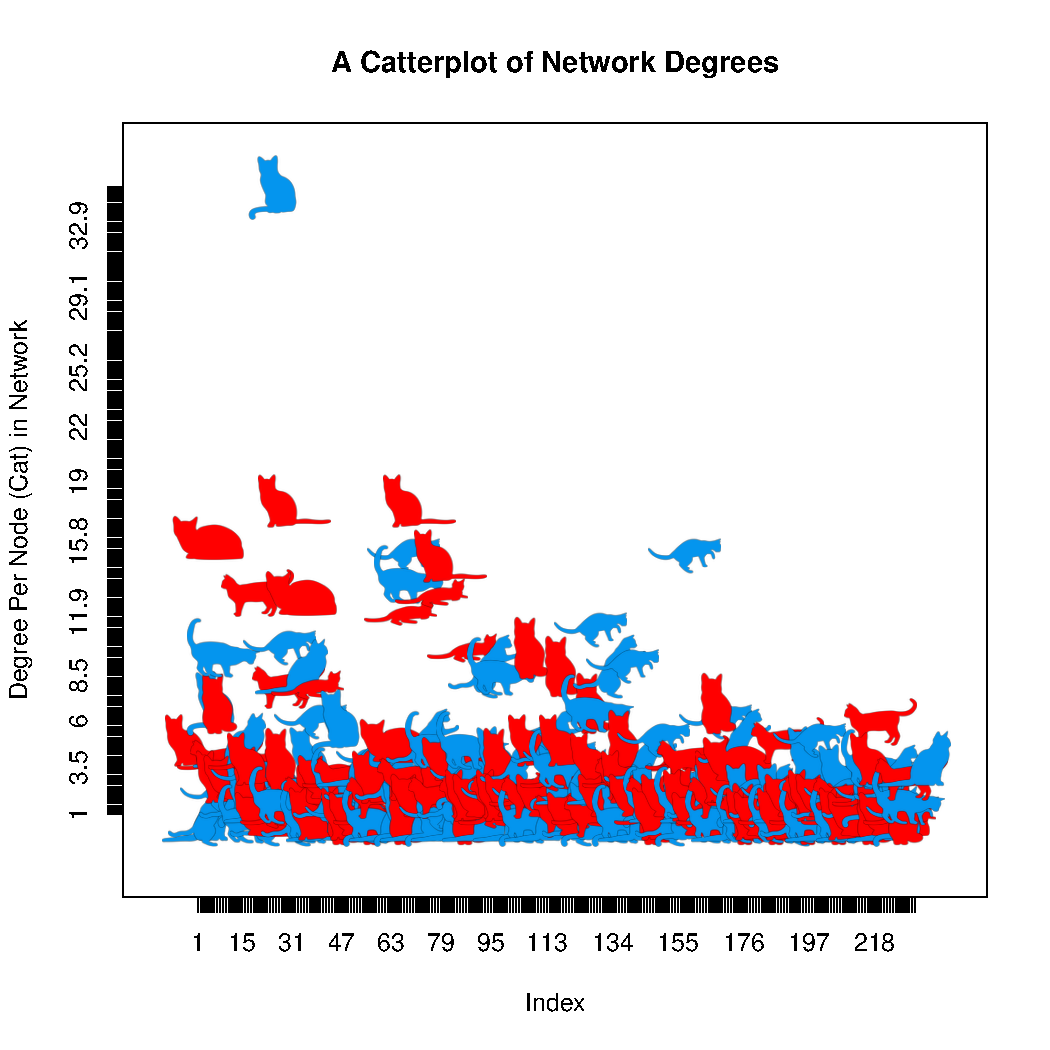
\includegraphics[width=5in]{figure/what-1} 

\end{knitrout}
\end{center}



%--------------------------------------
\clearpage
\section{Field Research Design: The Qualitative Alternative}

\subsection{Qualitative Value}

\subsection{Advice, Tools, Resources}

\subsection{How to Use Qualitative Evidence}




%--------------------------------------

\clearpage
\section{Content Analysis}

\subsection{The Protocol}

\subsection{The Coding Sheet}

\subsection{Reliability Measurements}

\subsection{Analysis}




%--------------------------------------------------------------------
\clearpage
\section{Formal Modeling}

\subsection{How can Formal Modeling Help?} \index{DAG}

The late statistician George Box once said ``All models are wrong, but some are useful.'' Formal Modeling (which I'll sometimes call game theory synonymously) can be used to spell out the the particular assumptions leading to an emperical test. Instead of writing long-hand the history, studies, and assumptions that go alongside our theory we explicity state relevent ``variables'' in math notation leading right up to a logical emperical test. This has many obvious benefits, chiefly it diciplines one to be explicit with their assumptions (similar, but more involved than DAG plots from the causal inference chapter). Also, this allows for clear objections and revisions to be made by future scholarship. Indeed many models, such as Downs' ``Median Voter Theorem'' has been revised multiple times given the clear writing from the original mathematical formal modeling.

Of course Downs and others who use formal modeling are very frequently ``wrong,'' but the purpose of formal modeling is to do things more systematically and with more academic rigor than prior. Works of this nature become foundational, having long shelf-lifes, and become solid building blocks for future scholarship to sculpt.


\subsection{Components of Game Theory}

\hfill \\

\noindent \textbf{Utility, First Best, Nash Equilibrium, Comparative Static}

\index{utility}
\noindent To begin, utility is one's preferences for one thing over another. For example, prefering guns to butter:

$$ u_i(\textit{Guns}) = 10 ~~~~ u_i(\textit{Butter}) = 1 $$\\

\noindent Which, note, is the same as this \textit{utility function}:

$$ u_i(\textit{Guns}) = 8,675,309 ~~~~ u_i(\textit{Butter}) = 1,337 $$\\

One's \textit{expected utility} is the mathematical calculation of one's probability of each event happening multiplied by each utility per outcome.\footnote{pg. 339 of Bueno de Mesquita's ``Political Economy for Public Policy has a great example of this. }

\index{First Best} \index{Nash Equilibrium}
\noindent Considering the standard 2x2 matrix format:

  \begin{table}[h!]
  \centering
    \setlength{\extrarowheight}{2pt}
    \begin{tabular}{cc|c|c|}
      & \multicolumn{1}{c}{} & \multicolumn{2}{c}{Player $Y$}\\
      & \multicolumn{1}{c}{} & \multicolumn{1}{c}{$A$}  & \multicolumn{1}{c}{$B$} \\\cline{3-4}
      {Player $X$}  & $A$ & $(x,y)$ & $(x,y)$ \\\cline{3-4} % \multirow{2}* was in front of {player}
      & $B$ & $(x,y)$ & $(x,y)$ \\\cline{3-4}
    \end{tabular}
  \end{table}

The \textit{First Best} is the bolded sections given the best strategic decisions per potential choice by the other player.


  \begin{table}[h!] % here!
  \centering        % I guess this is the only way to center the table?
    \setlength{\extrarowheight}{2pt}
    \begin{tabular}{cc|c|c|}
      & \multicolumn{1}{c}{} & \multicolumn{2}{c}{Country $Y$}\\
      & \multicolumn{1}{c}{} & \multicolumn{1}{c}{Don't Arm}  & \multicolumn{1}{c}{Arm} \\\cline{3-4}
      {Country $X$}  & Don't Arm & $\textbf{4, 4} $ & 0,\textbf{3} \\\cline{3-4}
      & Arm & \textbf{3},0 & 1,1 \\\cline{3-4}
    \end{tabular}
  \end{table}

The \textit{Nash Equilibrium} is the ``first best of the first bests'' or where all players reach an equilibrium around one set of strategies -- even though they may not have the highest pay-off or reward for a particular player. Note that the process here for solving a 3x3 to NxN matrix is similar to the standard 2x2. Also the Nash Eqilibrium(a) can be solved algebraicly as well; graphically it is the intersection of two lines which represent the strategic continum a player has. A Nash Eqilibrium(a) can be notated by any given variable: $\theta^*$.

\index{subgame perfect Nash Equilibrium}
A variation of the Nash Equilibrium is the \textit{subgame perfect Nash Equilibrium}, or the regular Nash Eqilibria per subgame of a longer, more dynamic, game.

\index{comparative static}
Another term, the \textit{comparative static} is the component of a model that connects our theory to our emperics through game-theoretic reasoning. Typically the comparative static is deployed in papers to test hypotheses, arrive at novel findings, argue for an expansion of a particular model or theory, or just to describe a phenomenon with more precision than before.


\subsection{Popular Games as Examples}






\subsection{Structuring Your Own Formal Model}


%-----------------------------------------------------------------------
\clearpage

\section{Meta-Analysis}

Increasingly popular in the social sciences (and beyond!) is the ``analysis of analyses'' or meta-analysis.\footnote{A term coined by Gene Glass as far back as 1976; however the practice of meta-analysis can be found as far back as 1904 with notable statisticians such as Pearson and Fisher.} The practice, broadly speaking, involves the combination of many articles on a specific topic to see where the ``jury stands'' on the topic. This involves the combination of effect sizes, weighted by sample sizes and other important components of a papers methodology, controlling for any impending biases of the article (gender of the authors, or year the article was published as examples). While modern practice encourages the combination of effect sizes, early meta-analyses involved the combination of p-values to make theoretical statements about the given topic. These latter practices are still ongoing today, and are often met with criticism this is because of the popular misconception of p-values being a statement about seeing theory in data rather than the data being observed given the sharp null hypotheses. \index{p-values}

That is,

\begin{equation}
\text{Pr}(\text{data}| H_0 \text{true}) = \text{p-values}

\text{Pr}(H_0 \text{true} | \text{data}) =/= \text{p-values}
\end{equation}

Effect sizes will be calculated in the sections that follow.


\subsection{The Art of Comparison}

In academia especially, articles are compared and contrasted against each other all time time. This usually occurs in an articles ``literuature review'' section - often around a topic of a theoretically interesting puzzle or unanswered question that the research hopes to illuminate for the reader. However, these sorts of compartisons are often without recognition of bias, random sampling of selected readings, or without recognition of elite scholars being able to more easily market their results. In contrast to literary comparisons meta-analyses apply a more quantitative approach to article examination of a topic and often result in similar advantages.

To highlight this point, an article by Bushman and Rothstein (2012) notes that often biases occur when one group is given sugguestive and attractive paper titles when others get dull scientific sounding titles. If studnets receive brief training in meta-analysis these biases go away. The article hits home the importance of empericial literature comparisons when something as small as the article title can bias the interpretation of an articles results.

\subsection{Examples}


%-----------------------------------------------------------------------
\clearpage
\addcontentsline{toc}{section}{Further Reading:}


\begingroup
	\nocite{*}

	%\setlength{\bibsep}{12pt}

	%\setstretch{2}

	\bibliography{GLM}

	\bibliographystyle{apsr}

\endgroup


%\clearpage
%\bibliographystyle{plain}
%\bibliography{GLM.bib}
%\printbibliography




%-----------------------------------------------------------------------
\clearpage
\addcontentsline{toc}{section}{Index}
\printindex











\end{flushleft}
\end{document}
